%==============================================================================
% Plantilla LaTeX para Tesis de Pregrado
% Universidad Industrial de Santander
% Diseño e Implementación de un Agente en Espacio de Usuario para la Gestión
% Dinámica de Frecuencia (DVFS) en Sistemas Heterogéneos mediante Modelos
% Ligeros de Machine Learning
%==============================================================================
%
% ESTRUCTURA MODULAR (2026-09-04): el documento se dividió en un archivo
% maestro (este) que solo contiene preámbulo y front/back matter, más un
% capítulo por archivo bajo secciones/, todos incluidos vía \input. Editar
% un capítulo ya no requiere abrir el monolito completo; compilar sigue
% siendo `latexmk main.tex` desde este directorio.
%
% El capítulo 1 (Marco de referencia) se reconstruyó a partir de la versión
% ampliada y corregida en docs/libro/main_fase02.tex --- ese documento
% quedó fuera de alcance como fuente de Metodología/Resultados porque
% describe el proyecto de "selector de dispositivo CPU/GPU" declarado fuera
% del alcance aprobado (ver Plan_Detallado_Realineacion_Hyperion.md §7 y
% Seguimiento_Cambios_Plan_Director.md); su Marco Conceptual, en cambio, es
% extrapolable al proyecto real (clasificador compute/memory-bound) y se
% incorporó aquí, excluyendo únicamente las dos subsecciones específicas del
% selector de dispositivo (rango dinámico de potencia entre CPU/GPU y costo
% de despacho amortizado) y una mención puntual del EDP como variable
% objetivo directa. Marco Legal y Estado del Arte resultaron idénticos entre
% ambos documentos.
%
% ESTADO DEL DOCUMENTO (2026-08-14): Redactado completo con los resultados
% reales de la Fase 1. La campaña CPU de reemplazo terminó con 126/126
% combinaciones aceptadas y datos de clasificación limpios, pero la
% verificación posterior de frecuencia efectiva por ventana demostró que los
% límites escritos en sysfs no retenían el reloj bajo carga mientras el
% turbo global permanecía activo; por ello esa campaña no constituye todavía
% evidencia de seis estados DVFS efectivos. El catálogo GPU fue auditado y
% corregido por precisión aritmética; el mecanismo operativo
% `nvidia-smi -lgc` quedó validado bajo carga real en dos objetivos
% distintos, sin atribuir el resultado a una versión de driver, aunque la
% campaña GPU completa sigue pendiente. Capítulos de Resultados, Discusión y
% Conclusiones redactados con estos datos; las Fases 2-4 (clasificador,
% agente, evaluación EDP) quedan fuera de alcance y se incorporarán al
% cerrarse cada una.
%
% PENDIENTES MARCADOS EN EL TEXTO:
%   - Sección 1.2 (Marco legal): a definir por los autores.
%==============================================================================

\documentclass[12pt,oneside,spanish]{book}

%==============================================================================
% PAQUETES
%==============================================================================

\usepackage[utf8]{inputenc}
\usepackage[T1]{fontenc}
\usepackage[spanish,es-tabla]{babel}
\usepackage[margin=2.5cm]{geometry}
\usepackage{hyperref}
\usepackage{setspace}
\usepackage{fancyhdr}
\usepackage{graphicx}
\usepackage{booktabs}
\usepackage{longtable}
\usepackage{array}
\usepackage{amsmath}
\usepackage{amssymb}
\usepackage[numbers]{natbib}
\usepackage{multirow}
\usepackage{xcolor}
\usepackage{float}
\usepackage{rotating}
\usepackage{adjustbox}
\usepackage{tabularx}
\usepackage{ltablex}
\usepackage{tikz}
\usetikzlibrary{positioning,fit,backgrounds,arrows.meta,calc}
\usepackage[indent=2em]{parskip}

%==============================================================================
% CONFIGURACIÓN DE ESPACIADO
%==============================================================================

\onehalfspacing

%==============================================================================
% ENCABEZADOS Y PIES
%==============================================================================

\pagestyle{fancy}
\fancyhf{}
\fancyhead[R]{\thepage}
\setlength{\headheight}{14.5pt}
\renewcommand{\headrulewidth}{0pt}
\renewcommand{\footrulewidth}{0pt}

%==============================================================================
% CONFIGURACIÓN DE HIPERENLACES
%==============================================================================

\hypersetup{
    colorlinks=true,
    linkcolor=black,
    citecolor=black,
    urlcolor=blue,
    pdftitle={Diseño e Implementación de un Agente en Espacio de Usuario para la Gestión Dinámica de Frecuencia (DVFS) en Sistemas Heterogéneos mediante Modelos Ligeros de Machine Learning},
    pdfauthor={Yeison Adrián Cáceres Torres; Ricardo Andrés Pérez Porras},
    pdfcreator={LaTeX with hyperref},
    pdfproducer={pdfTeX}
}

%==============================================================================
% NUEVA DEFINICIÓN DE CAPÍTULOS Y SECCIONES
%==============================================================================

\renewcommand{\thechapter}{\arabic{chapter}}
\renewcommand{\theequation}{\arabic{chapter}.\arabic{equation}}
\renewcommand{\thefigure}{\arabic{chapter}.\arabic{figure}}
\renewcommand{\thetable}{\arabic{chapter}.\arabic{table}}

%==============================================================================
% INICIO DEL DOCUMENTO
%==============================================================================

\begin{document}


%==============================================================================
% PORTADA
%==============================================================================

\begin{titlepage}
    \centering
    \vspace*{1cm}

    {\Large \textbf{Diseño e Implementación de un Agente en Espacio de Usuario}}

    \vspace{0.3cm}

    {\Large \textbf{para la Gestión Dinámica de Frecuencia (DVFS) en Sistemas}}

    \vspace{0.3cm}

    {\Large \textbf{Heterogéneos mediante Modelos Ligeros de Machine Learning}}

    \vspace{2cm}

    {\large Yeison Adrián Cáceres Torres}

    {\large Ricardo Andrés Pérez Porras}

    \vspace{2cm}

    {\large Trabajo de Grado para Optar el Título de Ingeniero de Sistemas}

    \vspace{2cm}

    {\large \textbf{Director}}

    {\large Gilberto Javier Díaz Toro}

    {\large Doctor en Ingeniería}

    \vspace{\fill}

    {\large Universidad Industrial de Santander}

    {\large Facultad de Ingenierías Físico-Mecánicas}

    {\large Escuela de Ingeniería de Sistemas e Informática}

    {\large Bucaramanga}

    {\large 2026}

\end{titlepage}

%==============================================================================
% PÁGINA DE AGRADECIMIENTOS
%==============================================================================

\chapter*{Agradecimientos}
\addcontentsline{toc}{chapter}{Agradecimientos}

\vspace{1cm}

% [PENDIENTE: redactar agradecimientos]

%==============================================================================
% RESUMEN
%==============================================================================

\chapter*{Resumen}
\addcontentsline{toc}{chapter}{Resumen}

\vspace{1cm}

\noindent\textbf{Título:} Diseño e Implementación de un Agente en Espacio de Usuario para la Gestión Dinámica de Frecuencia (DVFS) en Sistemas Heterogéneos mediante Modelos Ligeros de Machine Learning.

\medskip

\noindent\textbf{Autores:} Yeison Adrián Cáceres Torres; Ricardo Andrés Pérez Porras.

\medskip

\noindent\textbf{Palabras Clave:} DVFS; eficiencia energética; computación de alto rendimiento; modelo Roofline; telemetría microarquitectónica; aprendizaje automático supervisado.

\vspace{0.5cm}

\noindent\textbf{Descripción:}

El consumo energético constituye hoy una restricción estructural para el escalamiento de la computación de alto rendimiento (HPC), particularmente en nodos heterogéneos que integran CPU y aceleradores gráficos. El Escalado Dinámico de Voltaje y Frecuencia (DVFS) es el principal mecanismo de control disponible a nivel de hardware, pero su aprovechamiento efectivo depende de decidir, durante la ejecución, cuál punto operativo conviene según el comportamiento de la carga. Los gobernadores nativos del sistema operativo deciden a partir de la utilización agregada del procesador, una señal que no distingue si el rendimiento está limitado por la capacidad aritmética del núcleo o por la transferencia de datos desde memoria; en el segundo caso, sostener la frecuencia máxima incrementa el consumo sin una mejora proporcional del tiempo de ejecución.

Este trabajo propone el diseño, la implementación y la evaluación de un agente en espacio de usuario que infiere el régimen de ejecución de la aplicación a partir de telemetría microarquitectónica y traduce esa inferencia en decisiones discretas de DVFS sobre CPU y GPU, con el objetivo de optimizar el Producto Energía--Retardo (EDP) sin incurrir en una penalización severa del rendimiento ni en una sobrecarga de inferencia que anule el beneficio energético.

El desarrollo se organiza en cuatro fases: caracterización de cargas y construcción del conjunto de datos; entrenamiento y selección de un clasificador supervisado ligero; implementación del servicio de control; y validación experimental frente a los gobernadores nativos de Linux. El presente documento reporta el instrumento de medición y el protocolo experimental construidos durante la primera fase, cuyo aporte metodológico central es un procedimiento reproducible para etiquetar ventanas de ejecución como \textit{compute-bound} o \textit{memory-bound} mediante una calibración empírica del modelo Roofline sobre la plataforma de medición, con trazabilidad explícita de la calidad de cada observación.

% [PENDIENTE: al cerrar las Fases 2-4, incorporar aquí las cifras de
%  desempeño del clasificador, ahorro energético y EDP obtenidos.]

%==============================================================================
% ABSTRACT
%==============================================================================

\chapter*{Abstract}
\addcontentsline{toc}{chapter}{Abstract}

\vspace{1cm}

\noindent\textbf{Title:} Design and Implementation of a User-Space Agent for Dynamic Frequency Management (DVFS) in Heterogeneous Systems through Lightweight Machine Learning Models.

\medskip

\noindent\textbf{Authors:} Yeison Adrián Cáceres Torres; Ricardo Andrés Pérez Porras.

\medskip

\noindent\textbf{Keywords:} DVFS; energy efficiency; high performance computing; Roofline model; microarchitectural telemetry; supervised machine learning.

\vspace{0.5cm}

\noindent\textbf{Description:}

Energy consumption has become a structural constraint on the scaling of high performance computing (HPC), particularly on heterogeneous nodes that combine CPUs and graphics accelerators. Dynamic Voltage and Frequency Scaling (DVFS) is the main control mechanism available at the hardware level, but exploiting it effectively requires deciding, at run time, which operating point suits the current workload behaviour. Native operating system governors base that decision on aggregate processor utilisation, a signal that does not distinguish whether performance is limited by the arithmetic capability of the core or by data transfer from memory; in the latter case, sustaining maximum frequency raises power draw without a proportional improvement in execution time.

This work proposes the design, implementation and evaluation of a user-space agent that infers the execution regime of an application from microarchitectural telemetry and translates that inference into discrete DVFS decisions over CPU and GPU, aiming to optimise the Energy--Delay Product (EDP) without incurring a severe performance penalty or an inference overhead that cancels the energy benefit.

The work is organised in four phases: workload characterisation and dataset construction; training and selection of a lightweight supervised classifier; implementation of the control service; and experimental validation against the native Linux governors. This document reports the measurement instrument and experimental protocol built during the first phase, whose central methodological contribution is a reproducible procedure for labelling execution windows as \textit{compute-bound} or \textit{memory-bound} through an empirical calibration of the Roofline model on the measurement platform, with explicit traceability of the quality of each observation.

%==============================================================================
% TABLA DE CONTENIDOS
%==============================================================================

\clearpage
\tableofcontents

%==============================================================================
% LISTA DE TABLAS
%==============================================================================

\clearpage
\listoftables

%==============================================================================
% LISTA DE FIGURAS
%==============================================================================

\clearpage
\listoffigures

%==============================================================================
% INTRODUCCIÓN
%==============================================================================

\chapter*{Introducción}
\addcontentsline{toc}{chapter}{Introducción}
\setcounter{chapter}{0}
\setcounter{equation}{0}
\setcounter{figure}{0}
\setcounter{table}{0}

En los sistemas de cómputo de alto rendimiento (HPC), el consumo energético se ha consolidado como una restricción crítica para el escalado sostenible, especialmente en arquitecturas heterogéneas CPU--GPU. En este contexto, el Escalado Dinámico de Voltaje y Frecuencia (DVFS) constituye el principal mecanismo de control a nivel de hardware, permitiendo ajustar los estados operativos de los procesadores para optimizar el compromiso entre consumo energético y tiempo de ejecución. Sin embargo, la efectividad de este mecanismo depende de la capacidad del sistema para adaptar dinámicamente la frecuencia al comportamiento cambiante de las aplicaciones, lo cual representa un desafío abierto en entornos HPC modernos.

En la literatura, este problema ha sido abordado principalmente mediante dos enfoques. Por un lado, los gobernadores de energía del sistema operativo, como \texttt{ondemand} o \texttt{schedutil}, emplean políticas reactivas basadas principalmente en la utilización del procesador, sin considerar la naturaleza microarquitectónica de la carga de trabajo, lo que limita su capacidad de adaptación a cargas de trabajo científicas dinámicas. Por otro lado, diversas propuestas han explorado estrategias heurísticas basadas en métricas microarquitectónicas, utilizando reglas deterministas para ajustar la frecuencia de operación. Aunque estos métodos presentan bajo \textit{overhead}, su dependencia de umbrales estáticos y su limitada capacidad de generalización reducen su efectividad en escenarios donde las fases computacionales varían rápidamente.

A pesar de estos avances, persiste una limitación fundamental: la incapacidad de los enfoques actuales para capturar de forma robusta las transiciones dinámicas entre regímenes \textit{compute-bound} y \textit{memory-bound}, así como para adaptarse a la heterogeneidad CPU--GPU sin intervención manual o ajuste específico por carga de trabajo. Esta brecha evidencia la necesidad de mecanismos de control más flexibles que permitan inferir el régimen computacional de la aplicación en tiempo de ejecución y tomar decisiones de escalado de frecuencia fundamentadas en el perfil de ejecución.

En este contexto, el presente trabajo propone el diseño e implementación de un agente en espacio de usuario basado en modelos ligeros de aprendizaje automático, capaz de clasificar en tiempo de ejecución las fases de una aplicación como \textit{compute-bound} o \textit{memory-bound} a partir de telemetría microarquitectónica. Con base en esta clasificación, el sistema ajusta dinámicamente la frecuencia de CPU y GPU con el objetivo de optimizar el Producto Energía--Retardo (EDP). Se espera que este enfoque permita mejorar la eficiencia energética en comparación con los gobernadores tradicionales de Linux, manteniendo una degradación controlada del rendimiento y un \textit{overhead} mínimo asociado a la inferencia.

%------------------------------------------------------------------------------
% PLANTEAMIENTO Y JUSTIFICACIÓN DEL PROBLEMA
%------------------------------------------------------------------------------

\section*{Planteamiento y justificación del problema}
\addcontentsline{toc}{section}{Planteamiento y justificación del problema}

Existe una ineficiencia energética estructural en la operación de los sistemas de alto rendimiento (HPC), especialmente en infraestructuras que integran aceleradores gráficos (GPU) para ejecutar aplicaciones científicas intensivas. Cuando una aplicación entra en una fase donde el procesamiento depende principalmente de la transferencia de datos desde memoria, mantener la CPU o la GPU a su frecuencia máxima no mejora el rendimiento de manera proporcional. En estas condiciones, los núcleos de cómputo permanecen parcialmente inactivos esperando datos, lo que genera un consumo energético elevado sin un beneficio equivalente en tiempo de ejecución. Esta desalineación entre demanda computacional y frecuencia operativa ha motivado el estudio del escalado de frecuencia como mecanismo para mejorar la eficiencia energética en aplicaciones científicas \cite{Simsek2024} y en sistemas de gran escala donde la gestión de potencia impacta el comportamiento global del sistema \cite{Costa2025}.

El problema se agrava por la naturaleza multifásica de las aplicaciones HPC, cuyo perfil de ejecución cambia a lo largo del tiempo de ejecución. En particular, estas aplicaciones alternan entre fases donde el rendimiento está limitado por la capacidad de cómputo del procesador (\textit{compute-bound}) y fases donde está restringido por la transferencia de datos desde memoria (\textit{memory-bound}). Esta distinción es crítica porque, en el régimen \textit{memory-bound}, incrementos de frecuencia tienden a producir mejoras marginales en el tiempo de ejecución, mientras aumentan el consumo energético; en contraste, en fases \textit{compute-bound} la frecuencia sí impacta el desempeño de forma más directa. Por ello, se han propuesto marcos de caracterización para identificar y clasificar estas fases en entornos HPC, con el fin de habilitar decisiones de control más informadas \cite{Antici2024,Calore2017}.

A partir de este contexto, la gestión eficiente de frecuencia no depende únicamente de la disponibilidad del mecanismo DVFS en el hardware, sino de la capacidad del sistema para decidir, en tiempo de ejecución, cuál configuración resulta más conveniente según el comportamiento de la carga. Aunque se han propuesto mecanismos automatizados para seleccionar frecuencias óptimas de GPU con el fin de mejorar la eficiencia energética sin comprometer significativamente el desempeño \cite{Ali2023}, persiste una brecha en la implementación de estrategias que integren de forma coordinada componentes CPU--GPU y que operen durante la ejecución de la aplicación, considerando además el costo computacional asociado al propio proceso de decisión.

Esta brecha resulta especialmente relevante en entornos académicos y científicos, donde el consumo eléctrico incide directamente en los costos operativos, la disponibilidad efectiva de recursos y la sostenibilidad institucional. En este contexto, contar con un mecanismo capaz de observar el comportamiento de la aplicación, inferir su fase de ejecución y ajustar la frecuencia de operación sin intervenir el código fuente constituye una alternativa con valor técnico y práctico.

Desde la perspectiva internacional, la literatura reciente ha mostrado avances en la optimización energética mediante escalado de frecuencia, gestión de potencia y caracterización de cargas HPC \cite{Simsek2024,Costa2025,Antici2024,Calore2017,Ali2023}. Sin embargo, a nivel nacional y regional, este tipo de soluciones aún no se encuentra ampliamente implementado en infraestructuras académicas de cómputo científico, particularmente bajo esquemas que combinen telemetría de bajo nivel, modelos ligeros de aprendizaje automático y control en espacio de usuario. En consecuencia, el problema no solo es técnicamente relevante, sino también pertinente en términos de aplicabilidad local.

A partir de esta necesidad de optimización energética en sistemas heterogéneos, se formula la siguiente pregunta de investigación que servirá como eje de desarrollo del proyecto:

\vspace{0.5cm}

\noindent\fbox{\parbox{0.97\textwidth}{%
\textbf{¿En qué medida el diseño e implementación de un agente en espacio de usuario, guiado por modelos ligeros de aprendizaje automático, permite ajustar la frecuencia de operación (DVFS) en sistemas heterogéneos CPU--GPU para reducir el consumo energético, sin que el costo de la inferencia computacional degrade el rendimiento global de la aplicación, en comparación con los gobernadores nativos de Linux?}
}}

\vspace{0.5cm}

%------------------------------------------------------------------------------
% OBJETIVOS
%------------------------------------------------------------------------------

\section*{Objetivos}
\addcontentsline{toc}{section}{Objetivos}

\subsection*{Objetivo General}

Caracterizar, diseñar, implementar y evaluar un agente en espacio de usuario basado en modelos ligeros de Aprendizaje Automático para el ajuste dinámico de frecuencia (DVFS) en sistemas heterogéneos CPU--GPU, con el propósito de maximizar la eficiencia energética en aplicaciones científicas sin inducir una penalización severa en su rendimiento global.

\subsection*{Objetivos Específicos}

\begin{enumerate}

    \item Caracterizar el comportamiento computacional y el consumo energético de cargas de trabajo representativas (intensivas en cómputo y en memoria) bajo distintos estados de frecuencia, recolectando telemetría de bajo nivel mediante contadores de rendimiento por hardware e interfaces de potencia estándar (Perf y RAPL para CPU y NVML para GPU).

    \item Entrenar y validar modelos clásicos de Aprendizaje Automático (tales como Árboles de Decisión o Bosques Aleatorios) que sean capaces de clasificar, en tiempo de ejecución y con baja latencia de inferencia, las fases de ejecución de las aplicaciones basándose en la telemetría extraída.

    \item Desarrollar un servicio de control (\textit{daemon}) en el espacio de usuario que interactúe de forma asíncrona con el sistema operativo, leyendo el estado de los contadores de hardware, ejecutando la inferencia del modelo clasificador y aplicando políticas proactivas de DVFS a través de las interfaces estándar del sistema operativo, en función de la fase de ejecución inferida por el modelo.

    \item Evaluar el impacto empírico del sistema propuesto mediante el cálculo del Producto Energía--Retardo (EDP), con el fin de determinar estadísticamente si el ahorro energético compensa la sobrecarga computacional (\textit{overhead}) derivado de la inferencia del modelo en comparación con los gobernadores nativos de Linux.

\end{enumerate}

\chapter{Marco de referencia}

\section{Marco Conceptual}
\label{sec:marco-conceptual}

El ajuste dinámico de frecuencia y voltaje parte de la relación entre el punto
de operación del hardware, la potencia consumida y el tiempo de ejecución. El
efecto de modificar ese punto depende del comportamiento de la carga, por lo
que resulta necesario establecer qué limita su desempeño y qué señales
permiten reconocer esa condición durante la ejecución. A partir de esta
relación se organiza el marco conceptual, comenzando por el modelo Roofline y
la caracterización de los regímenes \textit{compute-bound} y
\textit{memory-bound}, para continuar con la telemetría disponible en CPU y
GPU, los modelos ligeros utilizados para inferir ese comportamiento y los
mecanismos de control DVFS. Finalmente, se introduce el Producto
Energía--Retardo como referencia para relacionar el ahorro energético con el
efecto que una decisión de frecuencia produce sobre el tiempo de ejecución.

\subsection{Potencia CMOS y fundamento de DVFS}
\label{sec:marco-cmos}

La potencia consumida por un circuito CMOS incluye una componente estática,
asociada principalmente a corrientes de fuga, y una componente dinámica
producida por la conmutación de cargas capacitivas. Dado que DVFS modifica la
frecuencia y, según el estado operativo, también el voltaje de alimentación,
su efecto se relaciona de forma directa con la potencia dinámica, que puede
aproximarse como:

\begin{equation}
P_{\text{dyn}} = \alpha \cdot C \cdot V^{2} \cdot f
\end{equation}

donde $\alpha$ representa el factor de actividad, $C$ la capacitancia efectiva
conmutada, $V$ el voltaje de alimentación y $f$ la frecuencia de operación
\cite{Gonzalez1997}. La dependencia cuadrática respecto al voltaje explica por
qué una reducción del punto operativo puede disminuir de forma apreciable la
potencia, aunque ese beneficio no puede evaluarse sin considerar el tiempo de
ejecución. Una carga que pierde rendimiento al reducir la frecuencia puede
permanecer activa durante más tiempo y compensar parte del ahorro obtenido.
Esta relación física da origen al compromiso energía--rendimiento que debe
resolver una política DVFS.

\subsection{Modelo Roofline y regímenes de ejecución}
\label{sec:roofline}

El efecto de variar la frecuencia no es uniforme porque el rendimiento de una
carga puede estar condicionado por recursos distintos. El modelo Roofline
formaliza esta diferencia al relacionar la intensidad operacional con los
límites de cómputo y ancho de banda de memoria de la plataforma
\cite{Williams2009}. Su formulación básica es:

\begin{equation}
P = \min\left(P_{\text{pico}},\; I \cdot BW_{\text{pico}}\right)
\label{eq:roofline}
\end{equation}

donde $P_{\text{pico}}$ corresponde al rendimiento aritmético pico, $I$ a la
intensidad operacional y $BW_{\text{pico}}$ al ancho de banda pico de memoria.
Cuando el límite viene dado por $I \cdot BW_{\text{pico}}$, aumentar la
capacidad de cómputo no elimina la restricción impuesta por el movimiento de
datos y la carga se considera \textit{memory-bound}. Cuando el límite
corresponde a $P_{\text{pico}}$, el rendimiento queda ligado a la capacidad
aritmética y el régimen se considera \textit{compute-bound}.

\begin{figure}[H]
    \centering
    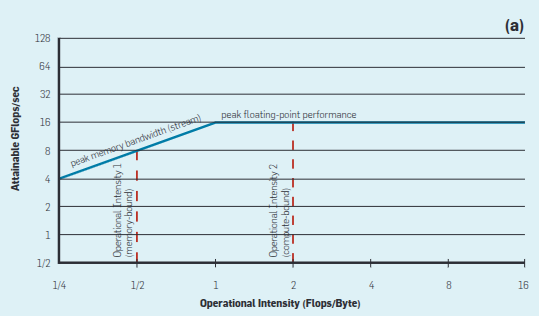
\includegraphics[width=0.72\textwidth]
        {figuras/fig_modelo_roofline_conceptual_williams2009.png}
    \caption[Modelo Roofline conceptual]{Modelo Roofline conceptual y relación
    entre el techo de ancho de banda de memoria y el techo de rendimiento de
    cómputo. Tomado de Williams et al. \cite[Fig.~1(a)]{Williams2009}.}
    \label{fig:modelo-roofline-conceptual}
\end{figure}

La separación entre ambos regímenes se encuentra en el \textit{ridge point},
obtenido al igualar las dos ramas del modelo:

\begin{equation}
I_{\text{ridge}} =
\frac{P_{\text{pico}}}{BW_{\text{pico}}}
\label{eq:ridge}
\end{equation}

Una intensidad inferior a $I_{\text{ridge}}$ sitúa la carga en la región
limitada por memoria y una intensidad superior en la región limitada por
cómputo \cite{Williams2009}. Este criterio es especialmente útil para el
proyecto porque permite construir una etiqueta a partir de una referencia
física del hardware, en lugar de asumir el régimen por el nombre del kernel o
por su comportamiento esperado. El punto de inflexión tampoco debe tratarse
como una constante universal. El techo de cómputo depende de la precisión
aritmética y puede variar con la frecuencia, mientras que el ancho de banda
pertenece a otro dominio y no necesariamente cambia en la misma proporción
\cite{Guerreiro2019,Ali2023}. Por ello, la interpretación de una carga debe
mantenerse vinculada a los techos correspondientes a la plataforma y al punto
operativo evaluado.
\label{sec:marco-ridge}

La intensidad operacional observada durante un intervalo $i$ se calcula como:

\begin{equation}
I_i =
\frac{\text{FLOPs}_i}{B_i^{\text{DRAM}}}
\label{eq:intensidad}
\end{equation}

$\text{FLOPs}_i$ representa el trabajo aritmético realizado y
$B_i^{\text{DRAM}}$ los bytes transferidos hacia o desde memoria principal
durante el mismo intervalo \cite{Williams2009}. Esta correspondencia temporal
es necesaria para conservar el significado físico de la razón. En CPU, el
trabajo aritmético puede obtenerse mediante eventos de rendimiento y el
tráfico hacia DRAM mediante contadores del controlador de memoria. En GPU, la
obtención de ambas magnitudes requiere una instrumentación de mayor detalle
que la telemetría ligera disponible durante la ejecución. Esta diferencia
explica por qué la referencia Roofline y las señales usadas posteriormente
para inferir el régimen no proceden necesariamente de la misma fuente.
\label{sec:intensidad}

\subsection{Telemetría microarquitectónica e instrumentación}
\label{sec:marco-telemetria}

La clasificación en línea requiere señales que reflejen el comportamiento del
hardware sin reproducir directamente el cálculo de la etiqueta Roofline. En
CPU, estas señales se obtienen principalmente mediante las Unidades de
Monitorización de Rendimiento, o PMU, que registran eventos asociados a la
ejecución. Parte de los contadores se reserva para eventos frecuentes, como
ciclos e instrucciones retiradas, mientras que otros son programables y
permiten seleccionar eventos definidos por la microarquitectura
\cite{IntelSDM2026}. Esta organización ofrece flexibilidad, pero también
impone un límite al número de eventos que pueden observarse al mismo tiempo.

% Se conserva aquí la figura PMU del archivo reescrito.

Cuando la cantidad de eventos solicitados supera los contadores físicos
disponibles, Linux puede multiplexarlos y estimar los conteos a partir del
tiempo durante el cual cada evento estuvo habilitado y realmente activo
\cite{Liu2024}. La relación entre \textit{time running} y
\textit{time enabled} permite reconocer esa situación y valorar si la lectura
mantiene una cobertura suficiente \cite{Liu2024,LinuxPerfEventOpen2026}. El
problema no es únicamente que existan pocos contadores, sino que una señal
observada de forma intermitente puede representar mal una carga cuyo
comportamiento cambia durante los periodos no medidos. Esta limitación
condiciona qué eventos resultan adecuados para alimentar un clasificador que
pretende operar sobre ventanas de ejecución.

La información tampoco procede de un único dominio. Los contadores de núcleo
registran eventos ligados a la actividad de los procesadores lógicos y
permiten derivar señales como IPC, tasa de fallos de caché, MPKI o ciclos de
espera. Los eventos \textit{uncore}, en cambio, cubren recursos compartidos
del zócalo, entre ellos el controlador de memoria y las interconexiones
\cite{IntelUncore2021}. Esta diferencia permite observar el tráfico que
alcanza DRAM, pero hace que su alcance y granularidad no coincidan
necesariamente con los contadores de núcleo. Para calcular intensidad
operacional, el trabajo aritmético y los bytes de memoria deben agregarse
sobre límites temporales compatibles antes de aplicar el criterio Roofline.
\label{sec:uncore}
\label{sec:ventanas}

Las métricas derivadas de los eventos de núcleo cumplen una función distinta a
la etiqueta. Un IPC bajo puede estar asociado con esperas, dependencias o
presión de memoria, mientras que los fallos de caché y los ciclos con
solicitudes de memoria pendientes aportan señales adicionales sobre la forma
en que progresa la ejecución \cite{Gregg2020,IntelPerfmon2026}. Ninguna de
estas variables demuestra por sí sola que una carga sea
\textit{memory-bound}. En Hyperion se utilizan como observaciones a partir de
las cuales el clasificador intenta aproximar una clase definida de manera
independiente mediante Roofline. Mantener esta separación evita convertir un
indicador microarquitectónico en una verdad física que no representa por sí
mismo.
\label{sec:marco-metricas-eficiencia}

Linux expone estas mediciones mediante \texttt{perf\_event}, que permite
acceder desde espacio de usuario a eventos de la PMU sin manipular
directamente sus registros \cite{LinuxPerfEventOpen2026,Weaver2015}. Para la
energía de CPU, Intel RAPL proporciona contadores acumulativos asociados a
dominios disponibles en la plataforma, entre ellos \textit{Package} y, cuando
existe soporte, DRAM \cite{David2010,Thamm2025}. La diferencia entre dos
lecturas permite obtener la energía correspondiente a un intervalo, aunque
esta medición representa los dominios expuestos por RAPL y no el consumo
eléctrico completo del nodo.
\label{sec:perfevent}
\label{sec:rapl}

La observabilidad de GPU tiene otra granularidad. NVML ofrece desde espacio de
usuario métricas agregadas de utilización, actividad de memoria, potencia,
energía y frecuencias de operación \cite{NVML2026}. Son adecuadas para
seguimiento continuo porque no requieren instrumentar cada kernel, pero no
proporcionan directamente los FLOPs y bytes necesarios para reconstruir la
intensidad operacional. Nsight Compute, por el contrario, puede perfilar
kernels CUDA con métricas de mayor detalle y obtener información suficiente
para caracterizar su posición en Roofline \cite{Nsight2026}. Su costo de
perfilado, que puede incluir varias pasadas sobre un mismo kernel, hace que su
papel sea distinto. \texttt{ncu} proporciona la referencia fuera de línea y
NVML las señales disponibles durante la inferencia, una separación que
mantiene la verdad de entrenamiento independiente de los proxies utilizados
por el modelo.
\label{sec:marco-nvml-ncu}
\label{sec:marco-interfaces}

\subsection{Control DVFS desde espacio de usuario}
\label{sec:marco-espacios-ejecucion}
\label{sec:dvfs-cpu}

El agente opera en espacio de usuario, mientras que el acceso directo a los
mecanismos del hardware permanece bajo control del kernel y de los
controladores del dispositivo \cite{Kerrisk2010,McCarty2015}. Esta separación
evita incorporar la lógica del proyecto como un módulo del kernel y permite
trabajar sobre interfaces estándar del sistema, aunque cada lectura,
inferencia y solicitud de frecuencia añade tiempo al lazo de decisión. La
utilidad del control depende, por tanto, de que ese costo sea pequeño frente a
la duración del comportamiento que se intenta aprovechar.

En CPU, Linux organiza la gestión de frecuencia mediante CPUFreq y los
mecanismos soportados por el procesador. Los \textit{governors} determinan
cómo se solicita un nivel de rendimiento, mientras que el controlador traduce
esa petición al hardware \cite{Hebbar2022,LinuxCPUFreq2026}. El
\textit{governor} \texttt{userspace}, cuando está disponible, permite que una
política externa participe en esa decisión, y las interfaces de CPUFreq
también exponen límites sobre los que puede actuar un servicio en espacio de
usuario. Hyperion se apoya en estas interfaces de control y se compara con
políticas nativas de referencia. \texttt{performance} mantiene una orientación
hacia niveles altos de rendimiento, \texttt{ondemand} responde a la carga
observada y \texttt{schedutil} incorpora información del planificador en la
selección de frecuencia \cite{Hebbar2022,LinuxCPUFreq2026}.

Una solicitud de frecuencia no equivale necesariamente al reloj que termina
usando el procesador. Mecanismos como \texttt{intel\_pstate}, HWP o Turbo
Boost pueden intervenir en el punto operativo efectivo según las condiciones
de ejecución \cite{LinuxIntelPstate2026,Hebbar2022}. Esta diferencia obliga a
distinguir entre la acción solicitada y el estado alcanzado, ya que la
comparación energética solo tiene sentido si el cambio atribuido a DVFS
ocurrió realmente. El mismo principio aplica al tiempo de transición. Una
decisión cuyo efecto tarda en materializarse puede perder utilidad cuando la
fase de la carga cambia antes de que el nuevo nivel llegue a aprovecharse.

En GPU, la relación entre frecuencia y rendimiento también depende del recurso
dominante. El dominio de procesamiento asociado a los SM y el dominio de
memoria no responden de la misma manera ante una variación del reloj
\cite{Guerreiro2019,Ali2023}. Una carga \textit{compute-bound} suele mostrar
mayor sensibilidad a la capacidad de procesamiento, mientras que en una carga
\textit{memory-bound} elevar el reloj de los SM puede aportar una mejora menor
si el movimiento de datos sigue imponiendo el límite. El régimen inferido
adquiere sentido para el control precisamente porque anticipa esa sensibilidad
y permite evitar cambios que añaden consumo sin una reducción proporcional
del tiempo.
\label{sec:dvfs-gpu}
\label{sec:dominios}

% Se conserva aquí la figura de dominios GPU del archivo reescrito.

El cambio de reloj en el acelerador tampoco es instantáneo. Entre la solicitud
y la estabilización del nuevo punto operativo existe una latencia que depende
del dispositivo y de la transición realizada \cite{Velicka2025}. Si ese
tiempo es comparable con la duración de la fase sobre la que se pretende
actuar, el beneficio potencial se reduce porque parte del intervalo transcurre
antes de alcanzar el estado deseado. La actuación DVFS en GPU debe
interpretarse, por ello, junto con la escala temporal de las fases y no
únicamente a partir de la clase inferida.

\subsection{Cargas de trabajo y calibración}
\label{sec:marco-cargas}

Las aplicaciones HPC combinan regiones con demandas diferentes sobre cómputo
y memoria, de modo que una medida agregada de toda la ejecución puede ocultar
cambios internos de comportamiento. Los kernels permiten aislar unidades de
trabajo con un patrón computacional definido, mientras que los benchmarks
aportan implementaciones reproducibles con diversidad algorítmica suficiente
para observar cómo responde la plataforma \cite{Williams2009,Gregg2020}. Su
procedencia no determina la clase. Una carga se considera
\textit{compute-bound} o \textit{memory-bound} a partir de la intensidad
operacional medida respecto al \textit{ridge point}, no porque la literatura
o el nombre del benchmark la describan de esa manera.

Los microbenchmarks cumplen una función distinta. Al reducir la ejecución a
operaciones controladas, permiten estimar propiedades de la plataforma como el
ancho de banda de memoria y el rendimiento aritmético \cite{Gregg2020}. Estas
mediciones sirven para construir los techos de Roofline y calibrar la
referencia con la que luego se etiquetan las cargas de caracterización. El
conjunto de entrenamiento se apoya así en benchmarks diversos, mientras que
los microbenchmarks proporcionan los límites físicos con los que se interpreta
su comportamiento.

\subsection{Clasificación supervisada ligera}
\label{sec:marco-ml-ligero}

La inferencia del régimen se plantea como un problema de clasificación
supervisada en el que una etiqueta conocida durante el entrenamiento se
relaciona con señales que también puedan observarse durante la operación del
sistema \cite{James2021}. En este caso, la etiqueta procede de Roofline y las
entradas corresponden a telemetría de bajo costo. La intensidad operacional y
las magnitudes que revelan directamente la regla utilizada para construir esa
etiqueta deben permanecer fuera del vector de características, pues incluirlas
convertiría la clasificación en una repetición del criterio de etiquetado y no
en una inferencia útil para el lazo de control.

El carácter ligero del modelo se define por su costo de operación y no por el
nombre del algoritmo. La regresión logística ofrece una referencia lineal,
mientras que los árboles de decisión representan relaciones no lineales
mediante reglas de partición sencillas \cite{James2021}. Random Forest y Extra
Trees combinan múltiples árboles para reducir la dependencia de una sola
partición, a cambio de evaluar varios estimadores durante la inferencia
\cite{Breiman2001,Geurts2006}. XGBoost construye el ensamble de forma
secuencial y permite representar interacciones más complejas entre
características \cite{Chen2016}. Comparar estas familias permite determinar si
el aumento de capacidad predictiva justifica también el costo temporal que
introduce en una decisión en línea.
\label{sec:marco-familias-modelos}

La evaluación debe reflejar tanto el desempeño global como el comportamiento
sobre cada clase. La matriz de confusión permite observar cómo se distribuyen
los errores entre \textit{compute-bound} y \textit{memory-bound}, mientras que
el $F_1$ combina precisión y sensibilidad y su promedio macro otorga el mismo
peso a ambas clases \cite{SokolovaLapalme2009}. Esta propiedad resulta útil
cuando la distribución de etiquetas no es uniforme, ya que evita que la clase
más frecuente determine por sí sola la lectura del resultado. Una línea base
mayoritaria proporciona además una referencia mínima para comprobar si las
señales de entrada contienen información discriminativa bajo el protocolo de
evaluación.
\label{sec:marco-evaluacion-clasificador}
\label{sec:marco-lineas-base}

La latencia de inferencia forma parte de esa evaluación porque cada predicción
consume tiempo dentro del ciclo de control. Un valor medio puede ocultar
ejecuciones ocasionalmente más lentas, por lo que percentiles como p95 y p99
permiten describir la cola de la distribución sin presentarla como un peor
caso absoluto \cite{Georges2007}. La elección de un modelo no puede separarse
por completo de este costo. Una mejora predictiva deja de ser atractiva si la
inferencia consume una fracción significativa del intervalo en el que todavía
puede aplicarse la decisión.
\label{sec:marco-costo-inferencia}

\subsection{Optimización de hiperparámetros y Optuna}
\label{sec:marco-optuna}

Además de los parámetros aprendidos durante el entrenamiento, cada familia de
modelos contiene hiperparámetros que condicionan su estructura o su proceso de
ajuste. La profundidad de un árbol, el número de estimadores de un ensamble o
la intensidad de regularización son ejemplos de valores que deben
seleccionarse antes de obtener el modelo final \cite{Bergstra2012}. Su
elección modifica tanto la capacidad de ajuste como la complejidad resultante,
de modo que comparar algoritmos sin considerar sus configuraciones puede
confundir las propiedades de una familia con una elección particular de
hiperparámetros.

Optuna organiza esta búsqueda mediante ensayos sucesivos o \textit{trials},
donde cada configuración se evalúa a partir de una función objetivo y los
resultados obtenidos orientan las propuestas posteriores \cite{Akiba2019}.
Entre los métodos disponibles se encuentra el \textit{Tree-structured Parzen
Estimator}, que utiliza los ensayos ya observados para modelar regiones
asociadas con mejores y peores resultados y concentrar parte de la exploración
donde existe mayor expectativa de mejora. La finalidad no es recorrer de forma
exhaustiva todas las combinaciones, sino asignar el presupuesto de evaluación
de manera más informada.

La optimización introduce, al mismo tiempo, un riesgo de adaptación a los
datos usados para escoger la configuración. Cuando la misma información
participa en la selección y en la estimación final del desempeño, la
evaluación puede quedar favorecida por el propio proceso de búsqueda. La
validación anidada separa ambas funciones mediante un nivel interno para
ajustar hiperparámetros y otro externo para estimar generalización
\cite{Cawley2010}. Si varias observaciones proceden de una misma familia
algorítmica, esa relación también debe preservarse durante la partición para
evitar que variantes estrechamente relacionadas aparezcan a ambos lados de la
evaluación \cite{Roberts2017}.

Esta separación estadística no corrige una fuga presente en las
características. Una variable derivada de la etiqueta, o suficientemente
cercana a la regla que la construye, puede ofrecer al modelo información que
no estaría disponible en una predicción real \cite{Kaufman2012}. En una
clasificación basada en Roofline, la distinción entre la fuente de verdad y la
fuente de inferencia debe mantenerse desde el diseño del conjunto de datos.
Optuna puede encontrar una configuración eficiente dentro del espacio
propuesto, pero no puede convertir en válida una entrada que ya contiene la
respuesta que el modelo intenta aprender.

\subsection{Producto Energía--Retardo}
\label{sec:marco-edp}

La reducción de potencia no implica necesariamente una mejora energética si el
tiempo de ejecución aumenta en una proporción suficiente para compensarla. Por
esta razón, la evaluación de DVFS requiere observar ambas magnitudes de forma
conjunta. El Producto Energía--Retardo, o EDP, expresa este compromiso mediante
\cite{Laros2013}:

\begin{equation}
EDP = E \cdot T
\end{equation}

$E$ representa la energía consumida y $T$ el tiempo de ejecución. Un valor
menor indica un compromiso más favorable bajo este criterio, pero la
formulación puede modificarse cuando se desea penalizar con mayor fuerza la
degradación temporal:

\begin{equation}
\mathrm{ED}^{n}\mathrm{P} = E \cdot T^{n}
\label{eq:ednp}
\end{equation}

Con $n=1$ se recupera el EDP clásico y con $n=2$ se obtiene ED$^{2}$P, donde
el tiempo adquiere mayor peso \cite{Laros2013,Ali2023}. La elección del
exponente modifica la forma en que se ordenan las configuraciones y debe
mantenerse explícita al comparar políticas. Para Hyperion, esta familia de
métricas permite valorar si una reducción energética justifica el cambio de
tiempo producido por la actuación DVFS, evitando interpretar potencia, energía
o rendimiento de manera aislada.

\section{Estado del Arte}
\label{sec:estado-del-arte}

La gestión energética en sistemas de alto rendimiento ha pasado de aplicar
reducciones de frecuencia de forma relativamente uniforme a considerar con
mayor detalle el comportamiento de cada carga. Este cambio responde a una
limitación conocida de DVFS. Reducir el punto operativo puede disminuir la
potencia, pero el resultado energético depende de cuánto se prolongue la
ejecución. Los trabajos más próximos a esta investigación pueden leerse, por
tanto, como una evolución desde la caracterización de esa sensibilidad hasta
mecanismos capaces de reconocer fases y actuar durante la ejecución.

Calore et al. \cite{Calore2017} analizaron el efecto de DVFS sobre una CPU
Intel Haswell y una GPU NVIDIA K80 utilizando kernels y una aplicación HPC
completa. Al modificar la frecuencia en regiones de ejecución observaron que
una misma configuración no ofrece el mismo compromiso entre energía y tiempo
para toda la aplicación. El trabajo establece una relación directa entre el
comportamiento local de la carga y la conveniencia de cambiar el punto
operativo, aunque la actuación depende de conocer previamente las regiones
donde debe aplicarse. El problema queda entonces planteado de una forma que
resulta relevante para Hyperion. Si las fases responden de manera distinta a
DVFS, el control necesita reconocer esas diferencias sin depender de
anotaciones específicas en cada aplicación.

Guerreiro et al. \cite{Guerreiro2019} abordaron esa necesidad desde la
caracterización de aplicaciones GPGPU. Su propuesta recoge métricas en una
configuración inicial y utiliza esa información para estimar cómo responderá
la carga ante otros estados de frecuencia de cómputo y memoria. Con ello
reducen la necesidad de recorrer exhaustivamente el espacio DVFS y muestran
que la sensibilidad de una aplicación puede anticiparse a partir de señales
del hardware. El enfoque, sin embargo, se concentra en caracterizar la
respuesta de una carga y no en seguir de manera continua las transiciones
entre fases \textit{compute-bound} y \textit{memory-bound}.

Ali et al. \cite{Ali2023} avanzaron en una dirección similar mediante modelos
de potencia y tiempo construidos a partir de métricas obtenidas en la
configuración predeterminada de la GPU. A partir de esas estimaciones
seleccionan frecuencias sin ejecutar cada alternativa y consideran de forma
conjunta el ahorro energético y la degradación del desempeño. En las
plataformas evaluadas reportaron reducciones promedio de energía de 29.6\% en
NVIDIA GA100 y 22.6\% en GV100, con pérdidas de rendimiento de 5.2\% y 4.7\%,
respectivamente. El resultado refuerza la idea de que una caracterización
limitada puede ser suficiente para orientar la selección de frecuencia, aunque
nuevamente la unidad de decisión es la carga caracterizada y no una sucesión
de fases detectadas durante la ejecución.

La identificación automática del régimen aparece de manera más directa en
MCBound, propuesto por Antici et al. \cite{Antici2024}. El trabajo formula la
separación entre cargas \textit{memory-bound} y \textit{compute-bound} como un
problema de clasificación a partir de datos de ejecuciones HPC. Sobre
información del supercomputador Fugaku, los autores reportaron un $F_1$ macro
de al menos 0.89, lo que muestra que el régimen puede inferirse mediante
señales observables sin depender exclusivamente de una clasificación manual.
MCBound se aproxima al problema predictivo de Hyperion, pero utiliza la clase
para caracterizar trabajos y no como entrada directa de una política que
modifique la frecuencia de CPU o GPU durante la ejecución.

Simsek et al. \cite{Simsek2024} estudiaron precisamente la actuación por
regiones en simulaciones astrofísicas ejecutadas sobre GPU. La instrumentación
de SPH-EXA les permitió modificar la frecuencia en puntos determinados y
reducir el consumo energético por GPU hasta en 7.82\%, con una degradación de
rendimiento cercana a 2.95\%. El resultado confirma que adaptar la frecuencia
dentro de una misma aplicación puede ser más conveniente que mantener un
estado uniforme, aunque la política continúa ligada a regiones conocidas del
código. La diferencia frente a una estrategia basada en telemetría es
importante, porque en esta última la frontera entre comportamientos debe
detectarse a partir de lo que el hardware expone durante la ejecución.

DRLCAP, presentado por Wang et al. \cite{Wang2024}, lleva esta idea hacia un
control \textit{online} basado en aprendizaje por refuerzo profundo. El marco
detecta cambios de fase y ajusta límites de frecuencia de GPU durante la
ejecución, con una reducción media de energía del 22\% y menos de 3\% de
degradación del rendimiento en las arquitecturas estudiadas. Este antecedente
demuestra que una política aprendida puede intervenir en tiempo real, pero
adopta una solución más compleja y centrada en GPU. Hyperion parte de otra
restricción. La inferencia debe mantenerse ligera y la política debe poder
operar sobre un entorno heterogéneo donde CPU y GPU no comparten las mismas
fuentes de telemetría ni los mismos mecanismos de actuación.

La literatura revisada cubre, por separado, los componentes principales del
problema. Calore et al. muestran que la respuesta a DVFS cambia entre regiones,
Guerreiro et al. y Ali et al. relacionan telemetría con sensibilidad y
selección de frecuencia, MCBound demuestra que el régimen puede inferirse
mediante clasificación y los trabajos de Simsek et al. y Wang et al. muestran
distintas formas de actuación durante la ejecución. La separación entre estas
contribuciones deja espacio para estudiar una integración donde la clase
inferida funcione como contexto de una política DVFS y donde el costo de
observar, clasificar y actuar forme parte de la evaluación.

Esta integración también exige tratar CPU y GPU como dispositivos distintos y
no como dos instancias del mismo problema. La mayoría de los trabajos recientes
de predicción y control se concentra en GPU, mientras que Calore et al. ofrecen
una de las referencias que consideran ambos tipos de dispositivo
\cite{Calore2017}. En CPU, las PMU y los contadores \textit{uncore} permiten
observar señales que no tienen un equivalente directo en NVML. En GPU, el
perfilado detallado necesario para construir la referencia Roofline tiene un
costo incompatible con la inferencia ligera y debe separarse de la telemetría
utilizada durante el control. El aporte que se investiga en Hyperion se sitúa
en esa diferencia de observabilidad, utilizando una referencia física común
para definir el régimen, pero aceptando que las señales con las que se intenta
inferirlo y los mecanismos de frecuencia disponibles son distintos en cada
dispositivo.
\chapter{Metodología}
\label{cap:metodologia}

\section{Enfoque y diseño}
\label{sec:met-enfoque}

La investigación es cuantitativa, experimental y aplicada. Es experimental porque manipula de forma deliberada el estado de frecuencia de CPU y GPU sobre un conjunto controlado de cargas y observa su efecto sobre el tiempo, la energía y el Producto Energía--Retardo. Es aplicada porque su producto es un agente de software funcional cuya utilidad se evalúa empíricamente frente a gobernadores nativos del sistema operativo y del controlador de la GPU. El trabajo se organiza en cuatro fases encadenadas (Figura \ref{fig:met-fases}): la Fase 1 produce el conjunto de datos etiquetado; la Fase 2 entrena y valida los clasificadores y deriva las tablas de política; la Fase 3 implementa el agente; la Fase 4 lo evalúa. Los esquemas y cuadros de verificación complementarios se reúnen en el Anexo \ref{anexo:metodologia}.

\begin{figure}[H]
\centering
\begin{tikzpicture}[
    font=\footnotesize,
    fase/.style={draw, rounded corners=2pt, align=center, minimum height=1.5cm, text width=3.1cm, inner sep=4pt, fill=blue!7, draw=blue!45!black},
    dato/.style={draw, rounded corners=2pt, align=center, minimum height=0.9cm, text width=3.1cm, inner sep=3pt, fill=orange!10, draw=orange!55!black},
    flujo/.style={-{Latex[length=2.2mm]}, semithick},
]
    \node[fase] (f1) {\textbf{Fase 1}\\Caracterización\\y datos etiquetados};
    \node[fase, right=1.0cm of f1] (f2) {\textbf{Fase 2}\\Clasificadores\\y tablas de política};
    \node[fase, right=1.0cm of f2] (f3) {\textbf{Fase 3}\\Agente de control\\DVFS};
    \node[fase, right=1.0cm of f3] (f4) {\textbf{Fase 4}\\Evaluación\\frente a REF};
    \node[dato, below=1.0cm of f1] (d1) {Conjunto de datos\\CPU y GPU\\con etiqueta Roofline};
    \node[dato, below=1.0cm of f2] (d2) {Modelos ONNX\\y política de\\frecuencia};
    \node[dato, below=1.0cm of f3] (d3) {Procesos de CPU\\y de GPU con\\tres brazos};
    \node[dato, below=1.0cm of f4] (d4) {EDP, energía\\y exactitud de\\clasificación};
    \foreach \a/\b in {f1/f2,f2/f3,f3/f4} \draw[flujo] (\a) -- (\b);
    \foreach \a/\b in {f1/d1,f2/d2,f3/d3,f4/d4} \draw[flujo] (\a) -- (\b);
\end{tikzpicture}
\caption[Fases de la metodología]{Fases de la metodología y producto de cada una. Fuente: elaboración propia.}
\label{fig:met-fases}
\end{figure}

\subsection{Población, muestra y criterios de inclusión}

La población son las aplicaciones para sistemas heterogéneos CPU--GPU; se estudió una muestra intencional de cargas reproducibles con regímenes contrastantes. Cada carga debía verificar su resultado, exponer trabajo de punto flotante medible por el instrumento y admitir una etiqueta de intensidad operacional. La unidad de diversidad y de validación fue la familia algorítmica: variantes de tamaño del mismo algoritmo no se trataron como familias independientes. El catálogo y su cribado se detallan en el Anexo \ref{anexo:metodologia}.

\subsection{Plataforma experimental}

Todos los experimentos se ejecutan en un único nodo, con asignación exclusiva del gestor de recursos para que ninguna carga ajena comparta el procesador durante las mediciones (Tabla \ref{tab:met-plataforma}). La plataforma se eligió porque expone la energía por interfaz interna sin privilegios administrativos (RAPL) y un acelerador instrumentable con NVML. Las actuaciones de frecuencia de CPU se restringen a los procesadores lógicos delegados, los núcleos 0 a 5 de un zócalo y sus hilos hermanos, porque el dominio de frecuencia es el núcleo físico y escribir un solo hilo no fija el reloj (anexo, sección \ref{sec:dominios}).

\begin{table}[H]
\centering
\caption{Plataforma experimental.}
\label{tab:met-plataforma}
\small
\begin{tabular}{@{}>{\raggedright\arraybackslash}p{4.2cm}>{\raggedright\arraybackslash}p{9.6cm}@{}}
\toprule
\textbf{Componente} & \textbf{Descripción} \\
\midrule
CPU & 2 $\times$ Intel Xeon Gold 5315Y (Ice Lake-SP), 8 núcleos físicos por zócalo, 2 hilos por núcleo, 2 nodos NUMA \\
Frecuencia & \texttt{intel\_pstate}, 0.8 a 3.2~GHz (3.6~GHz con \textit{turbo} activo), dominio por núcleo físico \\
Energía de CPU & Intel RAPL, dominios de paquete y de DRAM por zócalo \\
GPU & NVIDIA A100 PCIe 40~GB, telemetría por NVML \\
Ejecución & Nodo en asignación exclusiva (Slurm) \\
\bottomrule
\end{tabular}
\end{table}

\subsection{Instrumento de medición}

El instrumento propio tiene dos capas (Figura \ref{fig:arquitectura-instrumento}). La capa inferior, en C++, lanza la carga como proceso hijo detenido antes de su primera instrucción, abre los contadores de hardware sobre ese proceso con herencia y solo entonces lo reanuda, de modo que ninguna instrucción queda fuera de la observación y la medida abarca todo el árbol de procesos e hilos de la carga. Un hilo productor lee los contadores a intervalos regulares y deposita las muestras en una estructura circular de un productor y un consumidor; un hilo consumidor, en otro procesador lógico, las persiste (Figura \ref{fig:muestreo-spsc}, anexo \ref{anexo:metodologia}). La capa superior, en Python, ejecuta la lógica experimental: interpreta el manifiesto de la campaña, verifica la plataforma, calibra, planifica cada combinación, aplica el estado de frecuencia, valida cada corrida y construye el conjunto de datos.

\begin{figure}[tb]
\centering
\resizebox{0.95\textwidth}{!}{
\begin{tikzpicture}[
    font=\small,
    st/.style={draw, rounded corners=1.5pt, align=center,
        minimum height=0.95cm, text width=2.35cm, inner sep=2pt},
    py/.style={st, fill=blue!7, draw=blue!45!black},
    cpp/.style={st, fill=orange!10, draw=orange!55!black},
    ar/.style={-{Latex[length=1.8mm]}, semithick},
    cr/.style={-{Latex[length=1.8mm]}, semithick, dashed},
    sub/.style={font=\tiny, text=black!70, align=center},
    zlab/.style={font=\tiny\bfseries, text=black!55},
]
    % ---------- Banda A: capa Python, preparación (izq -> der) ----------
    \node[py] (man)  {Manifiesto de\\campaña\\{\tiny manifest}};
    \node[py, right=0.35cm of man]  (pre)  {Verificaciones\\previas\\{\tiny preflight}};
    \node[py, right=0.35cm of pre]  (cal)  {Calibración\\Roofline\\{\tiny calibration}};
    \node[py, right=0.35cm of cal]  (plan) {Matriz, orden\\de ejecución\\{\tiny campaign}};
    \node[py, right=0.35cm of plan] (loop) {\textbf{Bucle por}\\\textbf{combinación}\\{\tiny runner, freqctl}};
    \draw[ar] (man) -- (pre);
    \draw[ar] (pre) -- (cal);
    \draw[ar] (cal) -- (plan);
    \draw[ar] (plan) -- (loop);

    % ---------- Banda B: capa C++, medición (der -> izq) ----------
    \node[cpp, below=1.7cm of loop] (exec)
        {Ejecutor de la carga\\{\tiny hijo detenido,}\\{\tiny adjuntado y reanudado}\\{\tiny kernel\_launcher}};
    \node[cpp, left=0.35cm of exec] (coll)
        {Colector y lectores\\{\tiny perf, uncore,}\\{\tiny RAPL, NVML}};
    \node[cpp, left=0.35cm of coll] (ring)
        {Estructura circular\\{\tiny (Figura \ref{fig:muestreo-spsc})}\\{\tiny spsc\_ring}};
    \draw[ar] (exec) -- (coll);
    \draw[ar] (coll) -- (ring);
    \draw[cr] (loop.south) -- node[left, sub]
        {invoca por subproceso;\\antes fija la frecuencia} (exec.north);

    % ---------- Banda C: capa Python, consolidación (izq -> der) ----------
    \node[py, below=1.9cm of ring] (val) {Validación de\\la corrida\\{\tiny validation}};
    \node[py, right=0.35cm of val]  (post) {Post-proceso\\{\tiny postprocess}};
    \node[py, right=0.35cm of post]  (data)
        {\textbf{Conjunto de datos}\\{\tiny windows, intervalos}\\{\tiny \textit{uncore}, fases GPU}};
    \draw[cr] (ring.south) -- node[right, sub]
        {muestras crudas\\{\tiny (samples.csv)}} (val.north);
    \draw[ar] (val) -- (post);
    \draw[ar] (post) -- (data);

    % ---------- zonas ----------
    \begin{pgfonlayer}{background}
        \node[draw=blue!35, fill=blue!3, rounded corners, inner sep=0.2cm,
            fit=(man)(loop), label={[zlab, blue!45!black]above left:Capa Python: preparación y planificación}] {};
        \node[draw=orange!45, fill=orange!4, rounded corners, inner sep=0.2cm,
            fit=(exec)(ring), label={[zlab, orange!55!black]above left:Capa C++: medición}] {};
        \node[draw=blue!35, fill=blue!3, rounded corners, inner sep=0.2cm,
            fit=(val)(data), label={[zlab, blue!45!black]below left:Capa Python: validación y consolidación}] {};
    \end{pgfonlayer}
\end{tikzpicture}
}

\caption[Recorrido de una campaña a través de las dos capas del instrumento]{Recorrido de una
campaña a través de las dos capas del instrumento. La capa Python prepara la campaña (banda
superior), invoca por subproceso el ejecutor de la capa C++ una vez por combinación de carga y
frecuencia (banda intermedia), y consolida las muestras crudas que este produce en el conjunto de
datos (banda inferior). La capa C++ concentra la medición sensible a la latencia; la capa Python,
la lógica experimental, donde priman la claridad y la trazabilidad. Fuente: elaboración propia.}
\label{fig:arquitectura-instrumento}
\end{figure}

La Tabla \ref{tab:met-senales} resume las señales. Los contadores de CPU se limitan a nueve eventos simultáneos, dimensionados contra el presupuesto de contadores físicos del nodo, verificado empíricamente, para evitar la multiplexación y su extrapolación. Una \textbf{ventana de muestreo} es el intervalo entre dos lecturas consecutivas; su contenido es la diferencia de las lecturas acumuladas. El tráfico a DRAM se mide con los contadores del controlador de memoria (\textit{uncore}), cuyo intervalo práctico es de 10~ms o más, ya que el manual de perf advierte de overhead crítico y desestabilidad sub-10~ms \cite{PerfMeasurementOverhead2026}. En GPU, el recolector solicita lecturas NVML cada 5~ms mediante \texttt{gpu\_interval\_ns=5\,000\,000}; sin embargo, la actualización física de los sensores del controlador tiene una cadencia efectiva aproximada de 100--120~ms. Por ello, las muestras NVML se usan como telemetría agregada y no como ventanas GPU con resolución de 5~ms.

\subsection{Modelo Roofline y etiquetado}
\label{sec:met-roofline}

La etiqueta de cada observación (\textit{compute-bound} o \textit{memory-bound}) resulta de comparar su intensidad operacional $I$ con el punto de inflexión del modelo Roofline (ecuación \eqref{eq:ridge}), calibrado en la plataforma por precisión aritmética y, en las campañas con barrido, por nivel de frecuencia. Los techos se calibran al inicio de cada campaña, con la misma asignación de núcleos que las corridas, mediante microbenchmarks de ancho de banda y de cómputo, y se contrastan con una referencia declarada. La etiqueta se deriva sin juicio manual, y la expectativa cualitativa de régimen que declara cada carga se usa solo como contraste.

Los dos dispositivos obtienen $I$ de forma distinta (Figura \ref{fig:met-etiqueta}). En CPU, los FLOPs se miden por ventana con los sub-eventos de \texttt{FP\_ARITH\_INST\_RETIRED} ponderados por el ancho vectorial (ecuación \eqref{eq:flops-medidos}), y los bytes con los comandos CAS del controlador de memoria; $I$ se calcula por intervalo, en vivo. En las campañas de GPU empleadas en este trabajo, NVML no proporciona una medición de FLOPs ni de bytes por ventana o por lanzamiento. Por ello, la intensidad operacional se caracteriza fuera de línea con Nsight Compute \cite{Nsight2026} (ecuación \eqref{eq:intensidad-gpu}) y se asocia a cada corrida. Una etiqueta con granularidad de fase requeriría combinar el perfilado de contadores con una traza temporal de lanzamientos mediante CUPTI, mecanismo que no forma parte de las observaciones aceptadas para este conjunto. Para un kernel determinista, con tamaño, precisión, entradas y configuración de lanzamiento fijos, esta caracterización se trata como una propiedad operacional estable tras verificar la convergencia entre los dos puntos de mayor trabajo, cuyo cambio relativo debe ser inferior al 1\%. Esta condición no afirma que el tráfico observado sea invariante ante cualquier configuración de ejecución. La caracterización distingue la precisión efectivamente ejercitada y excluye las cargas de aritmética entera o de precisión mixta no resoluble.

\begin{figure}[H]
\centering
\begin{tikzpicture}[
    font=\footnotesize,
    b/.style={draw, rounded corners=2pt, align=center, minimum height=1.0cm, text width=3.3cm, inner sep=3pt},
    cpu/.style={b, fill=blue!7, draw=blue!45!black},
    gpu/.style={b, fill=orange!10, draw=orange!55!black},
    et/.style={b, fill=green!10, draw=green!45!black},
    fl/.style={-{Latex[length=2.2mm]}, semithick},
    lb/.style={font=\scriptsize\bfseries, text=black!60},
]
    \node[cpu] (c1) at (0,1.5) {FLOPs por ventana\\(PMU)};
    \node[cpu] (c2) at (0,-0.1) {Bytes por intervalo\\(CAS del IMC)};
    \node[cpu] (c3) at (4.6,0.5) {$I$ por intervalo\\(en vivo)};
    \node[gpu] (g1) at (0,-2.0) {Nsight Compute\\(fuera de línea)};
    \node[gpu] (g2) at (4.6,-2.0) {$I$ fija por kernel\\(tras convergencia)};
    \node[et] (r) at (9.2,-0.75) {$I$ frente al punto\\de inflexión: etiqueta};
    \node[lb, anchor=south] at (2.3,1.85) {CPU};
    \node[lb, anchor=north] at (2.3,-2.7) {GPU};
    \draw[fl] (c1.east) -- (c3.west);
    \draw[fl] (c2.east) -- (c3.west);
    \draw[fl] (g1) -- (g2);
    \draw[fl] (c3.east) -- (r.north west);
    \draw[fl] (g2.east) -- (r.south west);
\end{tikzpicture}
\caption[Obtención de la etiqueta en CPU y en GPU]{Obtención de la etiqueta Roofline. En CPU la intensidad se mide en vivo por intervalo del controlador de memoria; en GPU se caracteriza una vez por kernel, fuera de línea. Fuente: elaboración propia.}
\label{fig:met-etiqueta}
\end{figure}

\section{Fase 1: recolección y caracterización}
\label{sec:met-fase1}

\subsection{Verificación previa y catálogo}

Antes de medir, una batería de verificaciones automáticas, parte del comando que lanza la campaña, confirma las capacidades del entorno, la integridad del catálogo y la disponibilidad de la instrumentación (Tabla \ref{tab:verificaciones-previas}, anexo \ref{anexo:metodologia}). Las verificaciones bloqueantes detienen la campaña antes de tocar el sistema: se prefiere no producir datos a producir datos cuya validez no puede sostenerse. El catálogo definitivo es una lista versionada y congelada de familias elegibles, tras un cribado con una rejilla de frecuencia reducida de tres niveles que descarta candidatos, comprueba la utilidad de su señal y estima su cobertura del plano Roofline. Cada clase debe quedar representada por al menos cinco o seis familias distintas por dispositivo. Con esto en mente, el conjunto de CPU reúne 30 familias, y el de GPU 16 (anexo, secciones \ref{sec:banco-candidatos} y \ref{sec:cribado}).

\subsection{Matriz experimental y control de sesgos}

La matriz resulta de combinar las cargas del catálogo, los estados de frecuencia (Tabla \ref{tab:frecuencias} del Anexo \ref{anexo:metodologia}) y las repeticiones independientes del binario. Los niveles se verifican contra los relojes soportados por el nodo. En CPU, fijar un nivel requiere acotar el rango por núcleo y desactivar el \textit{turbo} global para evitar ajustes autónomos del gestor de energía. Cada ventana se clasifica como válida, no confiable, no verificable (margen tras transición) o no aplicable (nivel nativo).

Para mitigar la latencia de asentamiento del reloj, la cual fue medida bajo carga en 10–11~ms para CPU y 70–80~ms para GPU, se verificó cada nivel dentro de una tolerancia de $\pm5\%$ y se aplicó un margen de guarda de 0.15~s al inicio y final de la región medible.

Las medidas contra el sesgo son cinco. Cada combinación se repite tres veces (validado empíricamente como suficiente). El orden de ejecución se aleatoriza con una semilla registrada en el manifiesto. Se incluyen repeticiones de una carga de referencia, cuya dispersión relativa señala inestabilidad del entorno. El eje de frecuencia de un dispositivo se mide con el otro dispositivo en su \textit{governor} nativo, porque fijar la CPU en su nivel mínimo mientras se barre la GPU alarga las cargas de GPU y contamina la comparación. Y toda campaña reanudable conserva una huella del protocolo, de modo que dos manifiestos con protocolos distintos no se mezclan (anexo, sección \ref{sec:matriz-sesgos}).


\subsection{Calidad de los datos y granularidad}

Ninguna observación se descarta en silencio. Cada ventana conserva una anotación de calidad (válida, sin diferencia previa, excluida por calentamiento, contadores degradados, intensidad indefinida, energía inválida o sin lectura de frecuencia) y el filtrado es una decisión del análisis. El transitorio de arranque de cada carga se identifica en dos etapas sobre una señal representativa del estado de carga (IPC en CPU, utilización en GPU): el primer instante desde el cual el coeficiente de variación se mantiene en 5\% o menos en dos ventanas móviles consecutivas y, como respaldo, un método de detección de puntos de cambio. Ese intervalo solo actúa como filtro posterior y nunca condiciona la adquisición. Cada corrida completa se valida además por integridad global: sin pérdidas en la estructura de muestreo, suma de verificación correcta y criterio de éxito propio cumplido (anexo, sección \ref{sec:calentamiento}).

La unidad de observación del entrenamiento se declara por dispositivo (Tabla \ref{tab:met-granularidad}), porque en ambos casos la ventana del instrumento no coincide con la unidad que posee una etiqueta con respaldo físico. En CPU es un \textbf{intervalo del controlador de memoria}, con las variables recalculadas sobre los deltas agregados del intervalo y no promediando cocientes. En GPU es una \textbf{corrida completa}, con agregados robustos (mediana, dispersión) de las muestras válidas posteriores al calentamiento. Las lecturas repetidas de una misma corrida no se tratan como ejemplos independientes.

\subsection{Reproducibilidad}

Cada campaña queda definida por un manifiesto declarativo bajo control de versiones (cargas, estados de frecuencia, repeticiones, período de muestreo, asignación de núcleos, semilla y referencias de calibración). Junto con los datos se persisten el perfil de capacidades del nodo, la calibración y los metadatos de cada corrida. Una campaña interrumpida se reanuda saltando las corridas ya aceptadas, protegida por la huella del protocolo (anexo, sección \ref{sec:reproducibilidad}).

\section{Fase 2: modelos de clasificación y política de frecuencia}
\label{sec:met-fase2}

\subsection{Formulación, variables y validación}

Se formula una clasificación binaria supervisada por dispositivo; la salida es la probabilidad de la clase \textit{memory-bound}. En CPU, las seis variables son cinco tasas derivadas de los contadores del intervalo (IPC, MPKI, tasa de fallos de caché, fracción de ciclos detenidos por memoria e instrucciones por segundo) y la frecuencia observada, conservada como covariable porque la misma carga puede cambiar de posición respecto del punto de inflexión cuando cambia el techo de cómputo. Antes de entrenar, se revisan las correlaciones entre las columnas candidatas. Los pares con correlación absoluta superior a 0.85 (común en la literatura), y la colinealidad restante, evaluada mediante el factor de inflación de la varianza, orientan el descarte de variables redundantes. El conjunto final se registra en un contrato versionado por dispositivo (anexo, sección \ref{sec:contrato-features}).

La validación es \textit{leave-one-familia-out}: en cada pliegue se retira por completo una familia, que no participa en el ajuste, la selección de representación ni la elección del umbral (Figura \ref{fig:met-lofo}). Las celdas de familia y clase se limitan a 1000 intervalos con una semilla fija, y cada observación se pondera de forma inversa al tamaño de su celda (peso medio uno), de modo que ninguna celda domina por volumen. La métrica principal es la exactitud balanceada por celda de familia y clase,
\begin{equation}
\mathrm{EB} = \frac{1}{|\mathcal{C}|}\sum_{(f,c)\in\mathcal{C}} \frac{a_{fc}}{n_{fc}},
\label{eq:met-eb}
\end{equation}
donde $\mathcal{C}$ es el conjunto de celdas observadas (cada combinación de familia $f$ y clase $c$), $|\mathcal{C}|$ es el número de celdas, $a_{fc}$ son los aciertos en cada celda y $n_{fc}$ las observaciones totales de esa celda. Está definida aunque una familia tenga una sola clase y no depende de la prevalencia. La incertidumbre se reporta por dos vías: cinco semillas de submuestreo, y remuestreo con reemplazo de las familias (2000 réplicas) para los intervalos de confianza del 95\% y las comparaciones pareadas.

\begin{figure}[H]
\centering
\begin{tikzpicture}[
    font=\footnotesize,
    b/.style={draw, rounded corners=2pt, align=center, minimum height=0.9cm, inner sep=3pt},
    ext/.style={b, fill=blue!7, draw=blue!45!black, text width=4.2cm},
    mid/.style={b, fill=orange!10, draw=orange!55!black, text width=4.2cm},
    sal/.style={b, fill=green!10, draw=green!45!black, text width=4.2cm},
    fl/.style={-{Latex[length=2.2mm]}, semithick},
]
    \node[ext] (a) {Pliegue externo:\\se retira la familia $f$};
    \node[mid, right=0.5cm of a] (b) {LOFO interno sobre las\\demás familias: elige\\el umbral $\tau$};
    \node[ext, right=0.5cm of b] (c) {Se ajusta el modelo\\en las demás familias};
    \node[sal, below=0.8cm of a] (e) {EB, cobertura\\y abstenciones};
    \node[sal, below=0.8cm of c] (d) {Se predice $f$ con\\la regla selectiva};
    \draw[fl] (a) -- (b); \draw[fl] (b) -- (c); \draw[fl] (c) -- (d); \draw[fl] (d) -- (e);
\end{tikzpicture}
\caption[Validación anidada por familia]{Validación anidada \textit{leave-one-familia-out}. La familia retirada no interviene en ninguna decisión de ajuste. Fuente: elaboración propia.}
\label{fig:met-lofo}
\end{figure}

\subsection{Decisión selectiva y calibración}

Con $p_i$ la probabilidad de \textit{memory-bound} y $q_i=\max(p_i,1-p_i)$ la confianza, la regla selectiva entrega la clase solo si $q_i\geq\tau$ y en caso contrario emite \textit{revisar}:
\begin{equation}
\widehat{y}_i=\begin{cases}
\textit{memory-bound}, & p_i\geq 0.5\ \land\ q_i\geq\tau,\\
\textit{compute-bound}, & p_i<0.5\ \land\ q_i\geq\tau,\\
\textit{revisar}, & q_i<\tau.
\end{cases}
\label{eq:met-selectiva}
\end{equation}
El umbral $\tau$ se elige sobre una rejilla mediante un LOFO interno, maximizando la exactitud balanceada por celda calculada únicamente sobre las observaciones aceptadas, con una cobertura media por celda mínima de 0.60. Las salidas \textit{revisar} se consideran abstenciones y se excluyen del cálculo de las métricas de clasificación sobre las predicciones aceptadas. Su efecto se cuantifica mediante la cobertura, definida como la proporción del total de observaciones para las cuales el modelo emite una clase. La confianza se evalúa además mediante el error de calibración esperado, que divide los valores de confianza en diez rangos de igual amplitud y compara, en cada rango, la confianza media con la proporción real de aciertos,
\begin{equation}
\mathrm{ECE} = \sum_{b=1}^{10} \frac{n_b}{N}\left|\mathrm{conf}_b - \mathrm{acc}_b\right|,
\label{eq:met-ece}
\end{equation}
donde $N$ es el número total de observaciones evaluadas, $n_b$ es el número de observaciones del rango $b$, $\mathrm{conf}_b$ es la confianza media de ese rango y $\mathrm{acc}_b$ es su proporción de aciertos.

\subsection{Comparación y selección de modelos}

Se compararon siete modelos bajo el mismo protocolo: una regla mayoritaria, un árbol de profundidad uno, uno de profundidad seis, regresión logística, \textit{random forest}, \textit{extra trees} y XGBoost, con hiperparámetros fijos. La búsqueda de hiperparámetros con Optuna se evaluó anidada en cada pliegue externo y se descartó: con un número limitado de familias, el criterio interno que maximiza no discrimina de forma confiable la configuración que generaliza mejor. Para explorar si el desempeño observado estaba limitado principalmente por la capacidad del modelo o por la información contenida en las variables se aplicaron cuatro diagnósticos complementarios. Entre ellos se evaluó un clasificador de vecinos más cercanos sin ajuste, utilizado para examinar la separabilidad local de las clases en el espacio de variables (anexo, sección \ref{sec:metodologia-limite-cpu}). La selección del modelo final se realizó después de comparar el desempeño bajo el protocolo LOFO y de verificar la invarianza de las variables frente a la acción del agente. Los modelos y umbrales seleccionados se reportan en el capítulo de resultados.

\subsection{Invarianza de las entradas frente a la acción del agente}
\label{sec:metodologia-invarianza-gpu}

La comparación por exactitud identifica candidatos que generalizan fuera de familia, pero un clasificador integrado en un controlador debe usar entradas que no cambien como consecuencia de su propia acción. En GPU se audita esa condición con dos pruebas sobre los datos ya disponibles. La prueba contrafactual sustituye el valor de una entrada potencialmente afectada por la actuación y cuantifica los cambios de predicción. La prueba de exclusión repite la validación LOFO sin dicha entrada. Toda variable que no supera ambas pruebas se excluye del contrato operativo.

Los modelos se vuelven a evaluar con el contrato de entradas resultante. La selección exige exactitud balanceada, calibración y cobertura suficientes bajo LOFO; la latencia de inferencia se informa como propiedad de implementación, mientras que la latencia completa desde la detección hasta la actuación se mide separadamente durante la evaluación del agente. En CPU se aplica la misma auditoría a la frecuencia observada, mediante una sustitución contrafactual coherente con el cambio de frecuencia que puede ejecutar el agente. Los resultados de ambas auditorías se presentan en las secciones \ref{sec:resultados-gpu-invarianza} y \ref{sec:resultados-cpu-frecuencia-contrafactual}.

\subsection{Derivación de la política de frecuencia}

La política de frecuencia se deriva de la campaña de la Fase 1, por separado del clasificador. Cada nivel se compara con REF sobre el mismo kernel y la ganancia agregada se estima por \textit{bootstrap} de kernels. La regla de elección se valida dejando una familia fuera; cualquier refinamiento se congela antes de probarse en familias externas. En GPU, los kernels próximos al punto de inflexión se marcan como ambiguos sin excluirlos. El emparejamiento, las pruebas y los criterios de refinamiento se especifican en el Anexo \ref{anexo:metodologia}.

\section{Fase 3: agente de control DVFS}
\label{sec:metodologia-fase3}

La Fase 3 no vuelve a entrenar clasificadores ni vuelve a escoger frecuencias. Recibe como entradas congeladas tres artefactos de la Fase 2: el modelo ONNX de cada dispositivo, su umbral de abstención y la tabla de política. El modelo y el umbral proceden de la validación LOFO y de la auditoría de invarianza. La tabla de política procede, de forma independiente, de la comparación pareada de EDP entre niveles de frecuencia. Esta separación evita que el desempeño del clasificador se interprete como evidencia de que una frecuencia determinada mejora el EDP, o que la política de frecuencia determine la selección del modelo. La Fase 3 implementa detección, decisión, actuación, coordinación y restauración con esos artefactos sin modificarlos; la Fase 4 evalúa el conjunto ya congelado.

\subsection{Arquitectura}
\label{sec:metodologia-agente-arquitectura}

El agente son dos procesos independientes en C++, uno por dispositivo, coordinados por una señal de un solo bit (Figura \ref{fig:met-agente}). Se separaron porque los bucles operan a escalas distintas (ventanas de milisegundos en CPU, fases de segundos en GPU), porque un fallo en uno no impide que el otro restaure el dispositivo que le corresponde, y porque los experimentos de un solo dispositivo no cargan la biblioteca de gestión del otro. Ambos leen los modelos, umbrales y tabla de política congelados al inicio de la ejecución; el lanzador los traduce a las banderas de cada proceso.

\begin{figure}[H]
\centering
\begin{tikzpicture}[
    font=\footnotesize,
    b/.style={draw, rounded corners=2pt, align=center, minimum height=1.0cm, inner sep=3pt, text width=4.6cm},
    cpu/.style={b, fill=blue!7, draw=blue!45!black},
    gpu/.style={b, fill=orange!10, draw=orange!55!black},
    tab/.style={b, fill=green!10, draw=green!45!black, text width=9.0cm},
    fl/.style={-{Latex[length=2.2mm]}, semithick},
    lb/.style={font=\scriptsize, align=center},
]
    \node[tab] (t) {Tabla de política y modelos ONNX (Fase 2)};
    \node[cpu, below left=1.0cm and -1.6cm of t] (c1) {\textbf{Proceso de CPU}\\contadores por ventana\\XGBoost, histéresis};
    \node[gpu, below right=1.0cm and -1.6cm of t] (g1) {\textbf{Proceso de GPU}\\NVML, ventana sostenida\\random forest, abstención};
    \node[cpu, below=0.9cm of c1] (c2) {Actuador de CPU\\rango por núcleo y turbo};
    \node[gpu, below=0.9cm of g1] (g2) {Actuador de GPU\\bloqueo de reloj};
    \draw[fl] (t) -| (c1); \draw[fl] (t) -| (g1);
    \draw[fl] (c1) -- (c2); \draw[fl] (g1) -- (g2);
    \draw[fl, dashed] (g1.west) -- node[lb, above] {señal de\\GPU activa} (c1.east);
\end{tikzpicture}
\caption[Arquitectura del agente]{Arquitectura del agente: dos procesos, una tabla de política compartida y una señal de coordinación. Fuente: elaboración propia.}
\label{fig:met-agente}
\end{figure}

Cada proceso admite los tres brazos de la Tabla \ref{tab:agente-brazos}. El brazo \textit{base} es la referencia contra la que se compara todo, y el brazo \textit{sombra} mide la sobrecarga del agente sin su efecto sobre el hardware.

\begin{table}[H]
\centering
\caption{Brazos del agente.}
\label{tab:agente-brazos}
\small
\begin{tabular}{@{}>{\raggedright\arraybackslash}p{2.2cm}>{\raggedright\arraybackslash}p{3.3cm}>{\raggedright\arraybackslash}p{7.3cm}@{}}
\toprule
\textbf{Brazo} & \textbf{Agente} & \textbf{Comportamiento} \\
\midrule
Base & No corre & El dispositivo queda bajo su \textit{governor} nativo (\texttt{intel\_pstate} con turbo en CPU, gestión automática del controlador en GPU) \\
Sombra & Muestrea, clasifica y decide & Registra cada decisión y nunca escribe sobre el hardware \\
Activo & Muestrea, clasifica, decide y escribe & Aplica la frecuencia decidida y restaura el estado al terminar \\
\bottomrule
\end{tabular}
\end{table}

\subsection{Detección de fase, decisión y parámetros}
\label{sec:metodologia-agente-gpu}

El agente de GPU delimita fases con la utilización NVML, reúne 3~s de actividad y decide una vez por fase. Si se abstiene, libera el reloj. El agente de CPU decide por ventana y exige 50 propuestas consecutivas antes de cambiar de nivel. Los umbrales y periodos se reúnen en la Tabla \ref{tab:met-parametros}; la máquina de decisión se verificó por separado de la biblioteca de inferencia.

\begin{table}[H]
\centering
\caption{Parámetros del agente.}
\label{tab:met-parametros}
\small
\setlength{\tabcolsep}{3pt}
\begin{tabular}{@{}>{\raggedright\arraybackslash}p{1.4cm}>{\raggedright\arraybackslash}p{3.1cm}>{\raggedright\arraybackslash}p{8.0cm}@{}}
\toprule
\textbf{Proceso} & \textbf{Parámetro} & \textbf{Valor y razón} \\
\midrule
GPU & Umbral de actividad & 5\% de utilización \\
GPU & Ventana sostenida & 3~s; una decisión por fase \\
GPU & Cadencia de muestreo & 50~ms \\
GPU & Umbral de abstención & 0.90 (cobertura media por celda $\geq$ 0.60); seleccionado en la Fase 2 (sección \ref{sec:resultados-gpu-invarianza}) \\
GPU & Permanencia mínima entre cambios & 3.7~s, 10 veces la latencia de conmutación medida en la Fase 3 (sección \ref{sec:resultados-agente-latencias}) \\
CPU & Umbral de decisión & 0.85; congelado en la Fase 2 (sección \ref{sec:resultados-cpu-selectiva}) \\
CPU & Histéresis & 50 ventanas consecutivas \\
CPU & Piso con GPU activa & 3.2~GHz; verificado en la Fase 3 (sección \ref{sec:resultados-agente-restauracion}) \\
\bottomrule
\end{tabular}
\end{table}

\subsection{Política, actuación y coordinación}
\label{sec:metodologia-agente-politica}

La Tabla \ref{tab:agente-politica} separa la política operativa derivada en la Fase 2 de las variantes experimentales de CPU. La salida operativa de la Fase 2 para CPU es \textit{no actuar} en ambas clases, por lo que no se presenta F0 ni F1 como recomendación de despliegue. Para comprobar que esa decisión no oculta un efecto al cerrar el lazo de control, la Fase 4 incorpora un brazo de CPU experimental que fija F0 en cómputo y F1 en memoria, y una variante \textit{activo-F0} que mantiene F0 en ambas. Estas variantes no actualizan la tabla derivada ni alteran el modelo; se comparan contra el \textit{governor} nativo.

\begin{table}[H]
\centering
\caption{Acciones del agente. Las filas de GPU provienen de la política derivada en la Fase 2; las filas de CPU son variantes experimentales evaluadas en la Fase 4.}
\label{tab:agente-politica}
\small
\setlength{\tabcolsep}{4pt}
\begin{tabular}{@{}>{\raggedright\arraybackslash}p{1.7cm}>{\raggedright\arraybackslash}p{3.0cm}>{\raggedright\arraybackslash}p{7.5cm}@{}}
\toprule
\textbf{Dispositivo} & \textbf{Clase} & \textbf{Acción} \\
\midrule
CPU & \textit{compute\_bound} & Fija F0 (3.2~GHz, turbo desactivado); experimental \\
CPU & \textit{memory\_bound} & Baja a F1 (2.9~GHz) con confianza mínima de 0.85; experimental \\
GPU & \textit{memory\_bound} & Fija el reloj en 1260~MHz (F1) \\
GPU & \textit{compute\_bound} & No actúa: libera el reloj al \textit{governor} nativo \\
GPU & \textit{revisar} (abstención) & No actúa: libera el reloj al \textit{governor} nativo \\
\bottomrule
\end{tabular}
\end{table}

El actuador de CPU reutiliza las reglas de restricción de rango por núcleo del módulo de la Fase 1 (delegados y hermanos de \textit{SMT}), desactiva el turbo global con el envoltorio administrativo del nodo y escribe los núcleos en paralelo. Registra el estado previo, verifica cada escritura por relectura, falla cerrado ante cualquier inconsistencia y restaura el estado inicial al terminar, incluso ante \texttt{SIGTERM} o \texttt{SIGINT}; su equivalencia con el módulo de la Fase 1 se comprobó con una prueba de paridad. El actuador de GPU fija y libera el reloj con la herramienta de administración del controlador, con la misma disciplina de restauración.

La coordinación entre procesos es una regla de protección distinta de la tabla de política. Cuando la señal de actividad GPU está presente, impone temporalmente un piso de CPU de 3.2~GHz y no espera la histéresis. No reclasifica la fase de CPU ni convierte F0 en una acción recomendada por la Fase 2. Se adopta para evitar que las señales de una CPU que espera a la GPU desencadenen una reducción de frecuencia que prolongue la fase GPU. La Fase 3 verifica que el piso se aplique y se restaure; su efecto sobre EDP se mide por separado en la Fase 4 con el brazo sin piso.

\subsection{Aplicaciones compuestas y verificación previa}
\label{sec:metodologia-agente-compuestas}

Las aplicaciones compuestas registran con el reloj monotónico las fronteras reales de fase para puntuar al agente (Tabla \ref{tab:agente-compuestas}). A usa familias vistas y B familias inéditas; una tercera aplicación alterna CPU y GPU. Cada fase supera los 3~s de observación y se separa de la siguiente por 1~s de reposo. Los kernels inéditos de GPU usan parámetros ampliados del mismo binario verificado para sostener la actividad.

\begin{table}[H]
\centering
\caption{Aplicaciones compuestas con verdad de fase.}
\label{tab:agente-compuestas}
\small
\setlength{\tabcolsep}{4pt}
\begin{tabular}{@{}>{\raggedright\arraybackslash}p{1.4cm}>{\raggedright\arraybackslash}p{2.0cm}>{\raggedright\arraybackslash}p{10.2cm}@{}}
\toprule
\textbf{Alcance} & \textbf{Aplicación} & \textbf{Fases (clase)} \\
\midrule
CPU & A (vistos) & \texttt{dgemm\_n2048} (\textit{compute}), \texttt{npb\_cg} (\textit{memory}) \\
CPU & B (inéditos) & \texttt{cpu\_xsbench\_omp} (\textit{memory}), \texttt{cpu\_rsbench\_omp} (\textit{compute}) \\
GPU & A (vistos) & \texttt{gpu\_cutlass\_simt\_dgemm\_n4096} (\textit{compute}), \texttt{gpu\_rajaperf\_stream\_triad} (\textit{memory}) \\
GPU & B (inéditos) & BabelStream con \texttt{--numtimes 1000} (\textit{memory}), \texttt{rodinia\_lavamd} con \texttt{-boxes1d 100} (\textit{compute}) \\
\bottomrule
\end{tabular}
\end{table}

Antes de la evaluación se verificó el agente por dispositivo y con ambos a la vez: latencia de conmutación, sobrecarga, restauración bajo terminación anómala inducida y cumplimiento del piso de coordinación (sección \ref{sec:resultados-agente}).

\section{Fase 4: validación experimental}
\label{sec:metodologia-fase4}

\subsection{Diseño de la matriz}
\label{sec:metodologia-fase4-matriz}

La matriz inicial compara el agente contra el \textit{governor} nativo en tres ejes: el alcance (solo CPU, solo GPU o ambos a la vez sobre una aplicación que alterna fases), el tipo de kernel (vistos frente a inéditos, que mide la brecha de generalización con las mismas celdas) y el brazo (Tabla \ref{tab:fase4-matriz}). El orden de las celdas se aleatoriza con semilla fija y cada una ejecuta la aplicación dos ciclos completos. El brazo \textit{sombra} aísla la sobrecarga del agente; \textit{activo-F0} y \textit{activo sin piso} se incluyen como brazos experimentales porque la política de CPU resultó \textit{no actuar} en la Fase 2 y se quiere medir si esa conclusión se sostiene con el agente en el lazo. La matriz inicial usó cinco repeticiones en el alcance conjunto y tres en los demás casos. Con tres observaciones por brazo, el análisis es descriptivo mediante razones de medianas y valores individuales; una comparación no apareada de tres contra tres no puede producir evidencia exacta bilateral inferior a 0.10.

\begin{table}[H]
\centering
\caption{Matriz experimental de la Fase 4.}
\label{tab:fase4-matriz}
\small
\setlength{\tabcolsep}{3pt}
\begin{tabular}{@{}>{\raggedright\arraybackslash}p{1.7cm}>{\raggedright\arraybackslash}p{6.3cm}>{\centering\arraybackslash}p{1.1cm}>{\centering\arraybackslash}p{1.3cm}>{\centering\arraybackslash}p{2.1cm}@{}}
\toprule
\textbf{Alcance} & \textbf{Brazos} & \textbf{Vistos} & \textbf{Inéditos} & \textbf{Repeticiones} \\
\midrule
CPU & base, sombra, activo, activo-F0 & A & B & 3 \\
GPU & base, sombra, activo & A & B & 3 \\
Conjunto & base, sombra, activo con piso, activo sin piso & A & B & 3 (5 en la matriz inicial) \\
\bottomrule
\end{tabular}
\end{table}

\subsection{Medición y análisis}
\label{sec:metodologia-fase4-medicion}

En todos los escenarios, cada celda registra duración, energía de CPU (RAPL de ambos paquetes) y energía de GPU (contador NVML) por separado. Así, el EDP del nodo, $\mathrm{EDP} = (E_{\mathrm{CPU}} + E_{\mathrm{GPU}})\,T$, se calcula y se desagrega después; también se calcula $E_{\mathrm{GPU}}\,T$. La ventana energética abarca desde el arranque de la aplicación hasta su fin, con los procesos del agente ya activos, por lo que incluye su sobrecarga. Cada celda verifica la finalización de la aplicación y de los procesos del agente que correspondan, y restaura los estados de frecuencia que modificó.

En la matriz y en el escenario E, las aplicaciones compuestas registran las fronteras de fase conocidas y las decisiones de cada proceso (instante, clase, confianza y escritura); la aplicación se fija a los núcleos 0 a 3 y se libera el reloj de GPU entre celdas. LAMMPS también se ejecuta en esos núcleos, pero sus fases son naturales y no se registran fronteras. CloverLeaf se ejecuta como un proceso CUDA Fortran continuo con ocho CPU asignadas; no se le impone ni se le atribuye una frontera de fase. Para CloverLeaf se conserva además la salida numérica, muestras NVML cada 250~ms y el estado de reloj antes y después de cada celda.

Para cada combinación de alcance, kernels y brazo se calcula la mediana de duración, energías y EDP y su razón frente al brazo \textit{base} (menor es mejor). En la matriz inicial conjunta, que tiene cinco observaciones no apareadas por brazo, el EDP se contrasta con Mann--Whitney bilateral. Los dos confirmatorios de cinco bloques, E-A y CloverLeaf, se analizan por bloque: se informan las razones por bloque y la prueba exacta bilateral de signos. Con cinco pares, incluso cinco diferencias del mismo signo dan $p=0.0625$, por lo que el valor se reporta sin declarar significancia al nivel 0.05.

La clasificación se puntúa contra las fronteras reales solo en las aplicaciones compuestas: cada decisión se atribuye a la fase que contiene su instante y se reportan correctas, erróneas y abstenciones por alcance, tipo de kernel y dispositivo, junto con la cobertura. La diferencia de exactitud entre A y B mide la generalización dentro de ese protocolo. En CPU las decisiones son por ventana, así que la exactitud se pondera por ventanas y no por fases. En LAMMPS y CloverLeaf se reportan las decisiones y la actuación observada, pero no una exactitud de clasificación, pues no existe una verdad de fase independiente con esa granularidad.

\subsection{Escenarios adicionales}
\label{sec:metodologia-fase4-escenarios}

Además de la matriz inicial, que se reporta completa y es la referencia, se ejecutaron los protocolos complementarios de la Tabla \ref{tab:fase4-mapa}; sus condiciones completas se conservan en la Tabla \ref{tab:fase4-escenarios} del Anexo \ref{anexo:metodologia}. Cada protocolo se fijó antes de sus mediciones y todos los ejecutados se reportan, cualquiera que sea su resultado. El escenario E se definió con el criterio de selección de sus familias (ganancia de EDP con F1 de al menos 10\% en la Fase 2, más una variante con familias no vistas) y se verificó con una corrida previa de una repetición por brazo antes de la matriz completa.

La referencia secundaria sin turbo se incorporó en las campañas complementarias C y E. En ese brazo no se inicia ningún daemon: se desactiva el turbo de CPU inmediatamente antes de la ventana de medición, se verifica el estado solicitado y se restaura al terminar la celda. Se ejecutan tres repeticiones para cada combinación de aplicación y alcance incluida. El control conserva el \textit{governor} nativo y el reloj nativo de la GPU, por lo que solo permite atribuir al turbo de CPU una diferencia entre referencias; no representa una frecuencia fija de GPU.

La Tabla \ref{tab:met-amenazas} resume las principales amenazas a la validez y la medida que la controla.

\begin{table}[H]
\centering
\caption{Mapa de los escenarios de la Fase 4. El protocolo completo se conserva en el Anexo \ref{anexo:metodologia}.}
\label{tab:fase4-mapa}
\small
\begin{tabular}{@{}p{3.1cm}p{10.3cm}@{}}
\toprule
\textbf{Escenario} & \textbf{Contraste principal} \\
\midrule
A & Matriz inicial por dispositivo, familias vistas e inéditas y brazo \\
C & Agente de CPU con un hilo de inferencia \\
E & GPU con fases largas de memoria, familias vistas (E-A) e inéditas (E-B) \\
REF sin turbo & Línea base secundaria para aislar el turbo de CPU \\
D & LAMMPS con cuatro entradas y fases naturales \\
F & Premedición diagnóstica de la solicitud de F1 fijo \\
Confirmatorio E-A & Cinco bloques con REF, sombra, agente y solicitud de F1 fijo \\
CloverLeaf & Cinco bloques con REF, sombra y agente en aplicación continua \\
\bottomrule
\end{tabular}
\end{table}

\chapter{Resultados}
\label{sec:resultados}

Este capítulo organiza la evidencia por dispositivo. Primero se presentan los resultados de la campaña final de CPU. Después se reportan la validación del instrumento GPU, el diagnóstico exploratorio de su primer conjunto de entrenamiento y el cambio posterior de la estrategia de medición. Esta distinción evita presentar resultados intermedios como conclusiones finales. Las tablas y figuras de sensibilidad, desglose y trazabilidad se conservan en el Anexo \ref{anexo:resultados-complementarios}; el cuerpo principal mantiene la evidencia necesaria para seguir cada conclusión.

\section{Resultados de CPU}
\label{sec:resultados-cpu}

El conjunto de CPU procede de una campaña que cubrió 49 configuraciones de kernel en el nivel nativo y nueve niveles fijos de frecuencia, con tres repeticiones por combinación, y sus 1470 corridas finalizaron aceptadas. En esta campaña, el warmup se calibró a partir de las ventanas medidas para cada kernel y el conjunto se reprocesó con esos valores; los transitorios fueron pequeños, con un máximo de 4.8\% de la duración de corrida y valores inferiores a 2\% en la mayoría de los kernels.

La unidad que alimenta el conjunto de entrenamiento CPU es el intervalo real de \textit{uncore} de aproximadamente 10~ms (sección \ref{sec:granularidad}). La Tabla \ref{tab:cpu-cobertura-conjunto} resume la cobertura obtenida después del filtrado de calidad. De 1\,424\,531 intervalos procesados, 1\,309\,755 cumplieron simultáneamente los criterios de telemetría y de frecuencia. Los restantes se conservaron para auditoría, pero no recibieron una etiqueta de entrenamiento.

\subsection{Composición de fase por kernel}
\label{sec:resultados-cpu-composicion}

Las cargas y su suite de origen se enumeran en la Tabla \ref{tab:catalogo}. La Figura \ref{fig:cpu-composicion-clase-kernel} muestra que el conjunto cubre ambos regímenes y conserva configuraciones próximas al \textit{ridge}.

\begin{figure}[H]
    \centering
    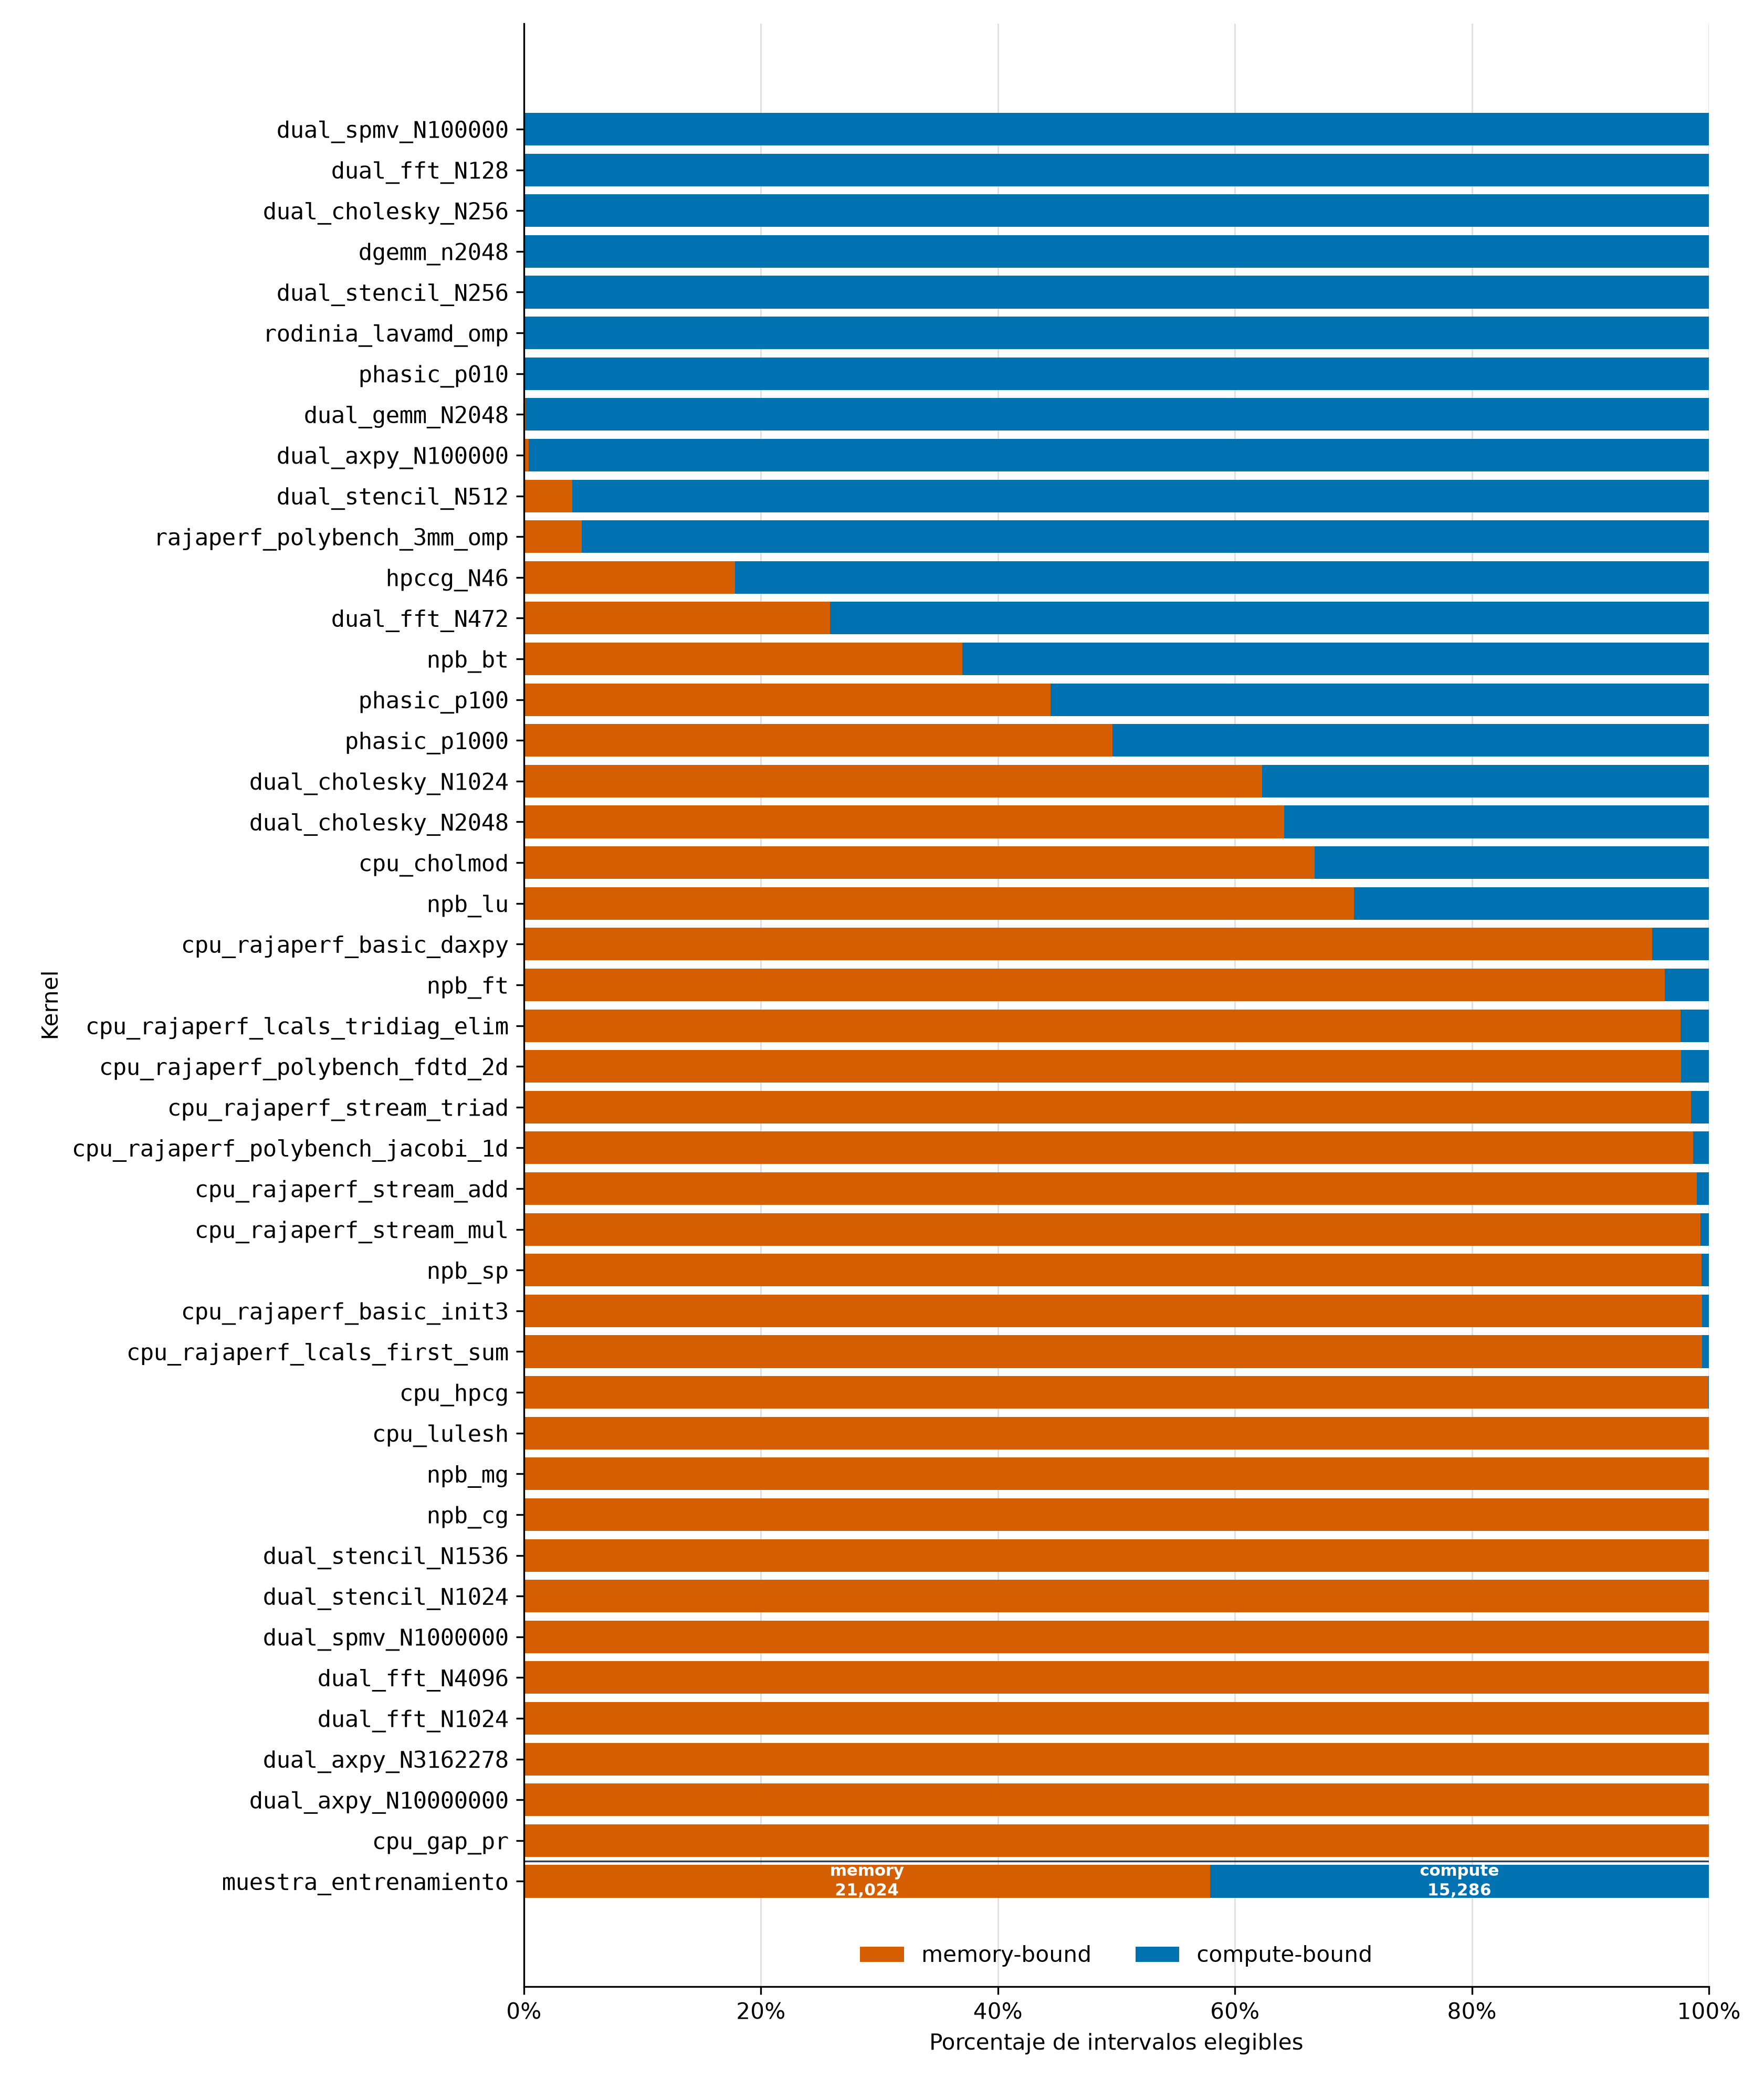
\includegraphics[width=0.60\textheight]
        {figuras/fig_cpu_composicion_clase_por_kernel_20260917.png}
    \caption[Composición de fase por kernel en CPU]{Porcentaje de intervalos elegibles clasificados \textit{compute\_bound} y \textit{memory\_bound} para cada configuración de kernel de la campaña CPU. La barra final resume la muestra usada por el clasificador, con 21\,350 intervalos \textit{compute\_bound} y 21\,108 intervalos \textit{memory\_bound}. Fuente: elaboración propia.}
    \label{fig:cpu-composicion-clase-kernel}
\end{figure}

La composición intermedia no se concentra en un solo algoritmo. \textit{npb\_bt}, \textit{npb\_lu}, \textit{cpu\_cholmod}, \textit{hpccg\_cpu\_N46}, las variantes \textit{phasic} y los tamaños dirigidos de FFT y Cholesky aportan intervalos de ambos regímenes. Estas configuraciones evitan que el conjunto quede limitado a ejemplos alejados del punto de inflexión.

Tres kernels de patrón de acceso irregular de Rodinia (\textit{kmeans}, \textit{srad} y \textit{particlefilter}) se midieron por separado y resultaron casi puramente \textit{memory-bound}; como no aportaban ejemplos \textit{compute-bound} ni mixtos, quedaron fuera del conjunto de entrenamiento por no añadir más que redundancia \textit{memory-bound}.


\subsection{Variación de la composición con la frecuencia}
\label{sec:resultados-cpu-frecuencia}

La proporción global de intervalos \textit{compute\_bound} aumentó desde 29.0\% en el nivel nativo hasta 46.4\% en F8, el nivel fijo más bajo. La Figura \ref{fig:cpu-composicion-clase-frecuencia} presenta esta variación. El resultado es consistente con un \textit{ridge} que disminuye cuando baja el techo de cómputo, de modo que una parte de los intervalos cercanos a la frontera cambia de etiqueta. La figura agrega todas las configuraciones y debe leerse junto con la composición por kernel, porque las cargas no aportan el mismo número de intervalos.

\begin{figure}[H]
    \centering
    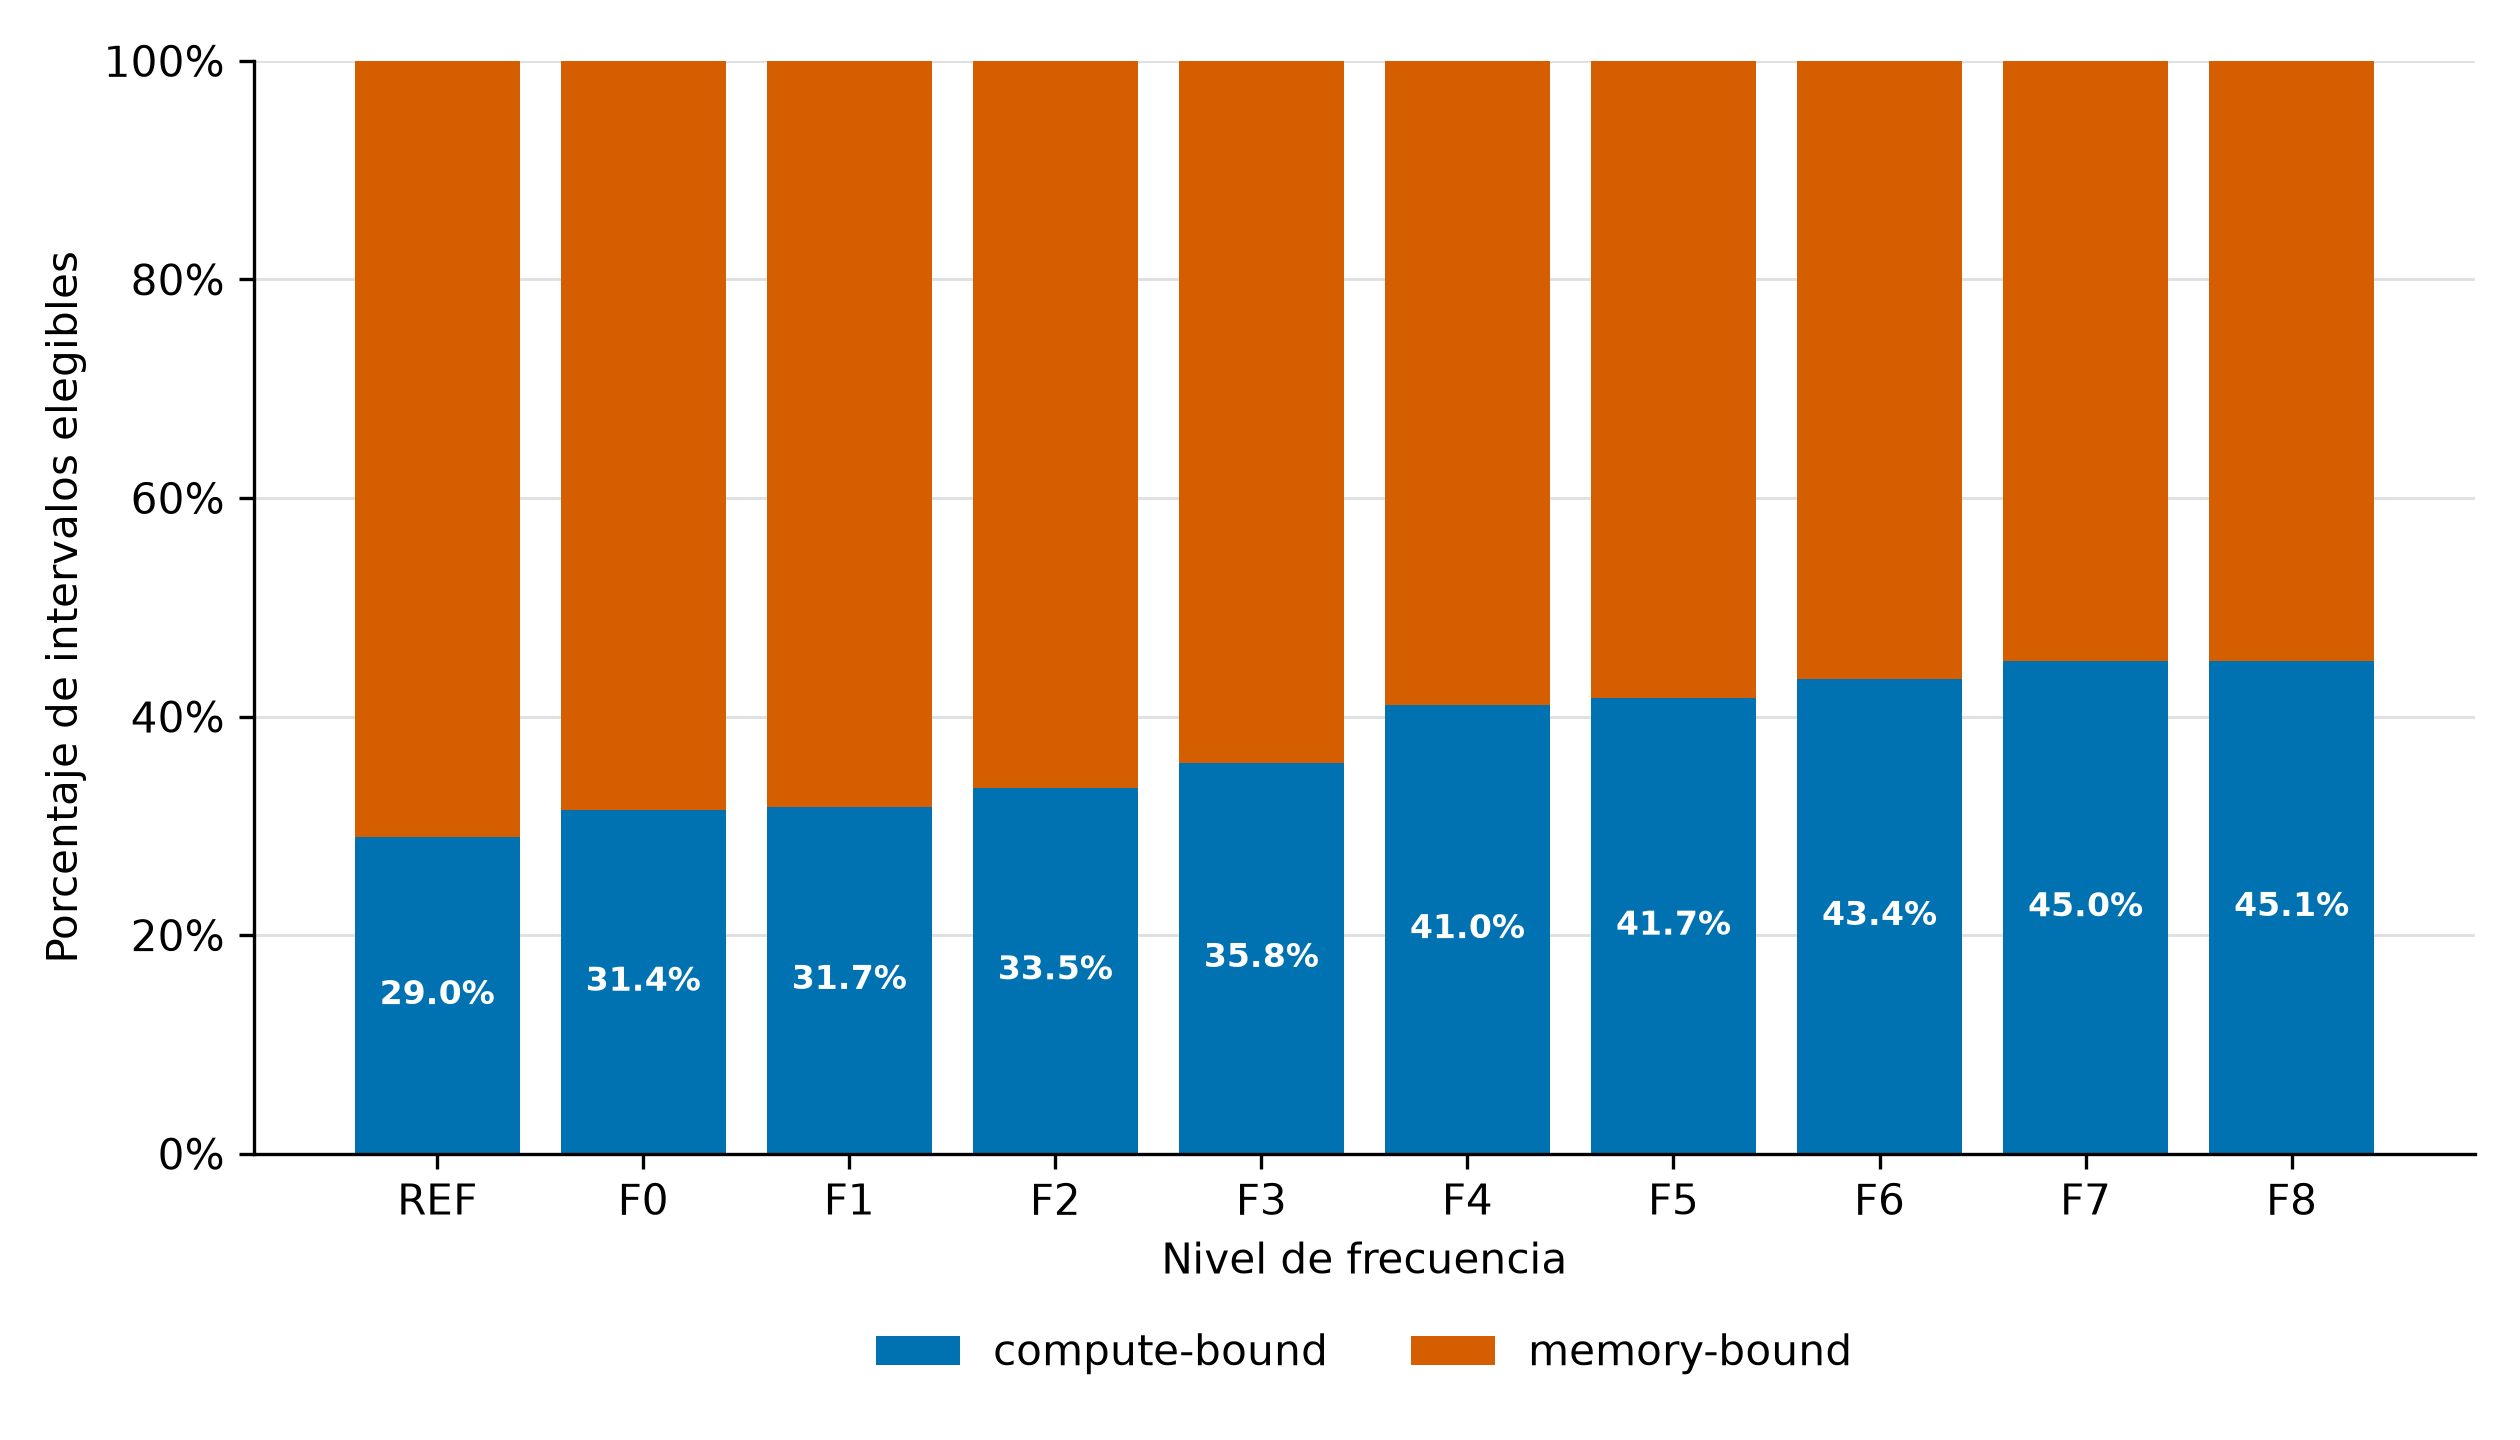
\includegraphics[width=0.9\textwidth]
        {figuras/fig_cpu_composicion_clase_por_frecuencia_20260917.png}
    \caption[Composición de fase por nivel de frecuencia en CPU]{Porcentaje de intervalos elegibles clasificados \textit{compute\_bound} y \textit{memory\_bound} en cada nivel de frecuencia de la campaña CPU. Fuente: elaboración propia.}
    \label{fig:cpu-composicion-clase-frecuencia}
\end{figure}


\subsection{Calidad del conjunto de datos}
\label{sec:resultados-cpu-dvfs}

Las 1470 corridas CPU se aceptaron con turbo desactivado y verificación del reloj observado dentro de $\pm5\%$. Se descartaron los márgenes de transición (unos 10~ms) y de inicio y final (0.15~s), además de las ventanas con frecuencia o telemetría no utilizable. En total, el 91.9\% de los 1\,424\,531 intervalos procesados quedó elegible (Tabla \ref{tab:cpu-rechazos}). La prueba de actuación confirmó que era necesario restringir también los hilos hermanos de \textit{SMT}.

\paragraph{Medición de bytes y etiqueta.}\label{sec:resultados-uncore}
Los bytes movidos en memoria se leen de los contadores de \textit{uncore} del controlador de memoria (sección \ref{sec:uncore}), y son la única fuente de bytes de la etiqueta. La etiqueta de cada intervalo compara los FLOPs medidos con esos bytes contra el \textit{ridge} calibrado para su nivel de frecuencia. La Figura \ref{fig:ridge-frecuencia} presenta cómo desciende el \textit{ridge} conforme baja la frecuencia. El presupuesto simultáneo es de nueve eventos de PMU y no diez, porque el vigilante NMI del sistema operativo reserva un contador físico por núcleo. Los contadores de \textit{uncore} son de alcance de sistema, por lo que cada campaña exige el nodo en exclusiva; con esa condición, la cadencia de intervalos se sostuvo en los $\sim$10~ms esperados a lo largo de toda una corrida de prueba. Antes de la campaña completa se ejecutaron dos campañas de humo a escala reducida (18 y 21 combinaciones) que ejercitaron el mismo camino de código y se aceptaron por completo; con clasificaciones coherentes: la multiplicación densa de matrices fue \textit{compute-bound} en el 100\% de sus ventanas y los kernels de NAS resultaron predominantemente \textit{memory-bound}.\label{sec:resultados-interferencia-uncore}

\begin{figure}[H]
\centering
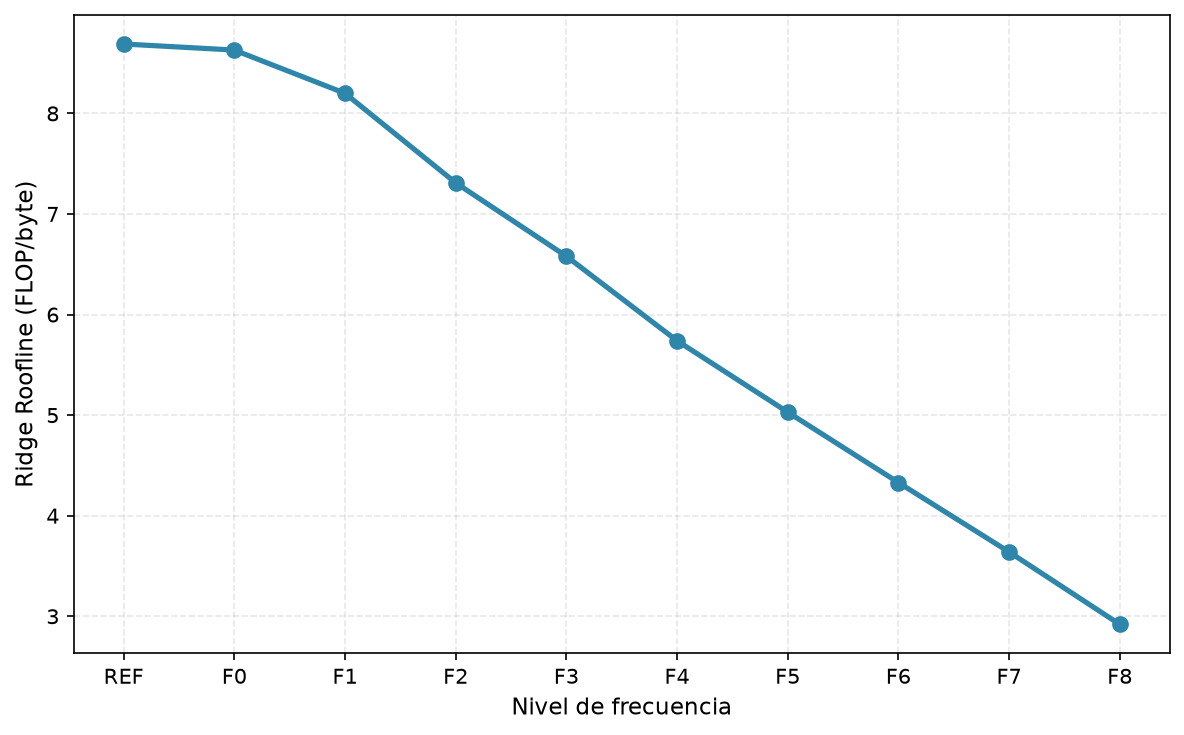
\includegraphics[width=0.6\textwidth]{figuras/fig_ridge_por_frecuencia_20260920.png}
\caption{\textit{Ridge} Roofline según el nivel de frecuencia CPU. El punto de inflexión desciende de 8.69~FLOP/byte en referencia nativa a 2.92~FLOP/byte en F8. Fuente: elaboración propia.}
\label{fig:ridge-frecuencia}
\end{figure}

La Figura \ref{fig:cpu-roofline-scatter} sitúa los intervalos del conjunto de entrenamiento directamente en el plano Roofline, contra el techo calibrado de cada nivel. Los FLOPs y bytes por intervalo no forman parte del vector de entrada del clasificador (sección \ref{sec:contrato-features}), por lo que esta vista se reconstruye aparte, sobre las mismas corridas de la campaña, y se muestra solo para REF y F8 como los extremos del rango de frecuencia. La nube \textit{memory-bound} queda, en su mayoría, bajo la rampa de ancho de banda a la izquierda del \textit{ridge}, y la nube \textit{compute-bound} bajo el techo plano de cómputo a la derecha; ambas quedan muy por debajo del techo teórico, porque los kernels reales sostienen una fracción de la tasa aritmética pico que un microbenchmark de registro alcanza (sección \ref{sec:roofline}). La franja de intervalos que cruza el \textit{ridge} en ambos sentidos es la misma ambigüedad que cuantifica la Figura \ref{fig:cpu-margen-ridge}.

\begin{figure}[H]
\centering
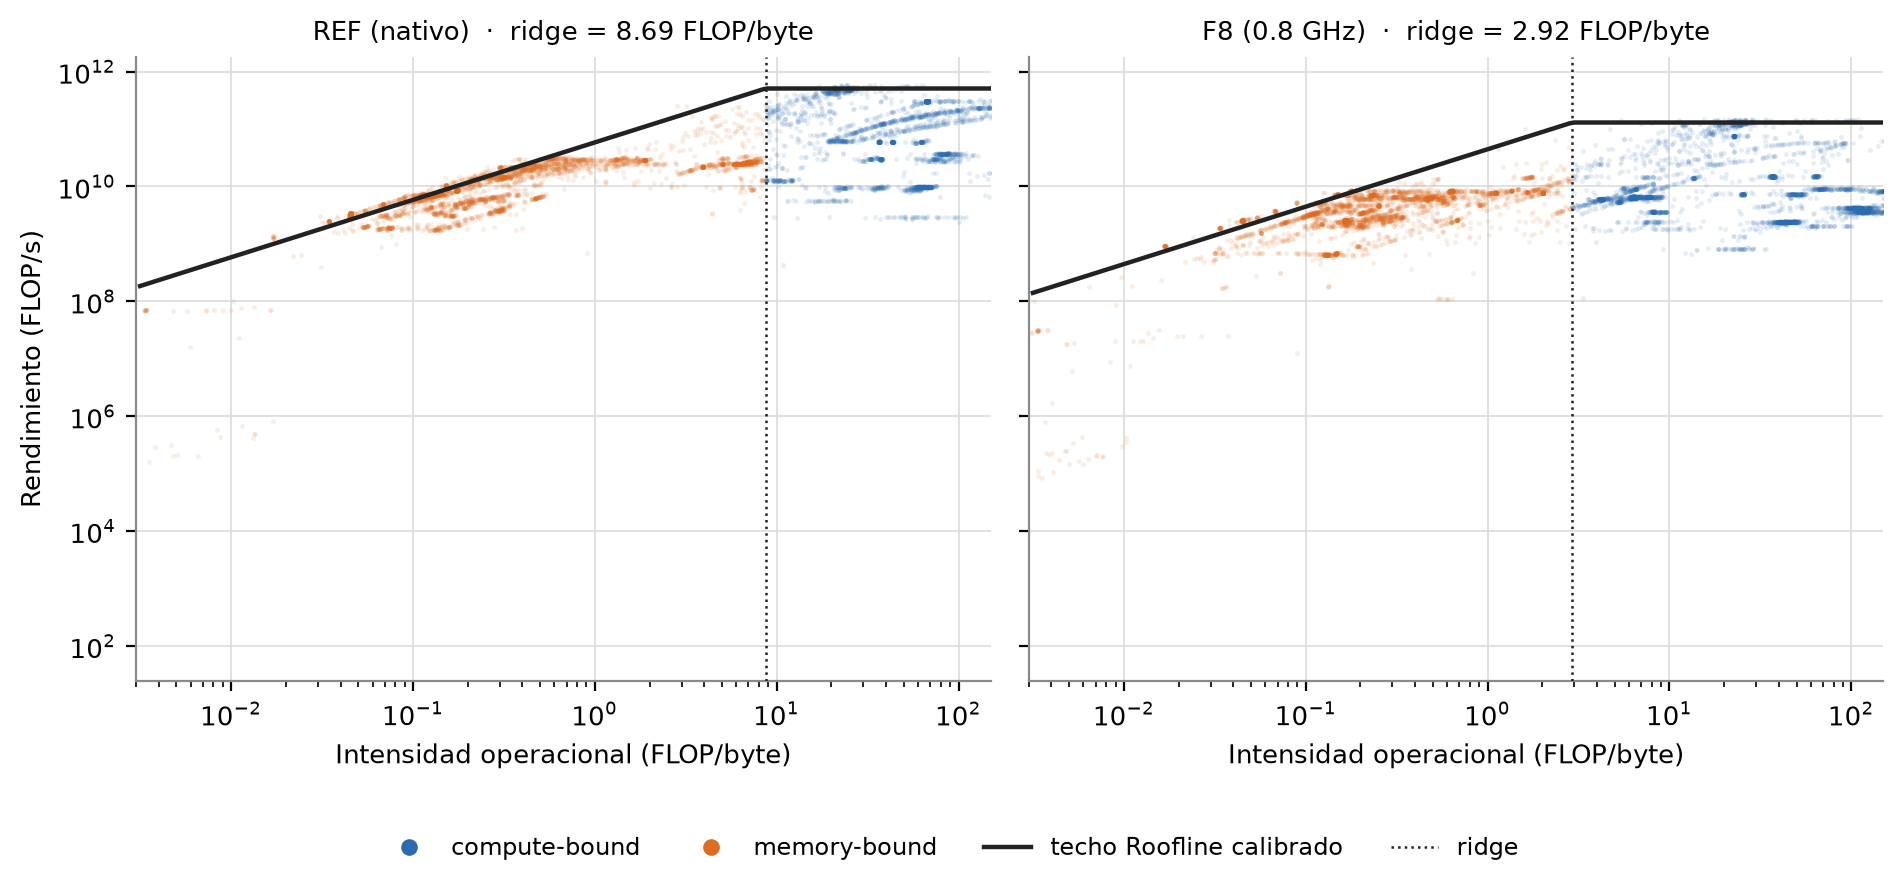
\includegraphics[width=0.98\textwidth]{figuras/fig_cpu_roofline_scatter_20260922.png}
\caption[Intervalos del conjunto de entrenamiento en el plano Roofline]{Submuestreo estratificado (4000 por nivel y clase, semilla 20260918) de los intervalos elegibles de REF y F8 en el plano intensidad--rendimiento, con el techo Roofline calibrado de cada nivel. Fuente: elaboración propia, reconstruido desde \path{training_cpu_intervals.csv} de la campaña \texttt{pacca\_cpu\_final\_20260913}.}
\label{fig:cpu-roofline-scatter}
\end{figure}

\paragraph{Validación de los techos Roofline.}\label{sec:resultados-ppico}
Los techos del modelo Roofline se calibraron de forma empírica sobre la propia plataforma (sección \ref{sec:roofline}). Para verificar esa calibración con un mecanismo independiente se empleó Intel Advisor, que contabiliza FLOPs y bytes mediante instrumentación binaria y no mediante contadores de PMU \cite{Advisor2026}. El ancho de banda calibrado coincide con el de Advisor dentro de 12 a 15\% (58.4 a 58.8~GB/s frente a 64.0 a 66.8~GB/s) y el techo de cómputo (417.8 a 555~GFLOP/s) es consistente con la referencia de Advisor, que midió 577.7~GFLOP/s sobre los mismos seis núcleos. El punto de inflexión del nivel nativo queda entre 7.0 y 9.3~FLOP/byte, compatible con los 8.69~FLOP/byte usados en la campaña, y desciende con el reloj hasta 2.92~FLOP/byte en F8, porque baja el techo de cómputo mientras el ancho de banda sigue limitado por memoria.


\subsection{Clasificador de fase en CPU}
\label{sec:resultados-cpu-clasificador}

Esta sección sigue el orden de construcción del clasificador: la muestra de entrenamiento, las variables de entrada, la elección del modelo, las métricas con que se evalúa y, por último, el resultado. El procedimiento está descrito en las secciones \ref{sec:metodologia-features-cpu} a \ref{sec:metodologia-congelacion-cpu}.

Dos convenciones se usan desde la primera cifra y se definen por completo solo en la sección \ref{sec:resultados-cpu-metricas}: toda evaluación sigue el protocolo \emph{dejar una familia fuera} (\textit{LOFO}), es decir, cada familia algorítmica se retira por completo, el modelo se ajusta con las 29 restantes y se evalúa exclusivamente sobre la retirada; y la métrica principal es la \textbf{exactitud balanceada por celda}, el promedio de la fracción de aciertos de cada combinación de familia y clase, que pesa cada celda por igual con independencia de cuántos intervalos aporte.

\subsubsection{Muestra de entrenamiento}
\label{sec:resultados-cpu-muestra}

El modelo CPU se ajusta con 42\,458 intervalos de 30 familias y un máximo de 1000 por celda de familia y clase; la evaluación usa todos los intervalos elegibles de la familia retirada (Tabla \ref{tab:cpu-flujo-modelo}). La Figura \ref{fig:cpu-muestreo-familia} muestra el submuestreo por familia. La sensibilidad entre topes de 100 y 30\,000 mantuvo la exactitud entre 0.720 y 0.739, sin tendencia creciente (Tabla \ref{tab:cpu-tope-muestreo}). La diferencia entre sortear por celda o repartir el tope entre niveles de frecuencia fue compatible con cero. La unidad de generalización sigue siendo la familia, no cada intervalo.


\begin{figure}[H]
    \centering
    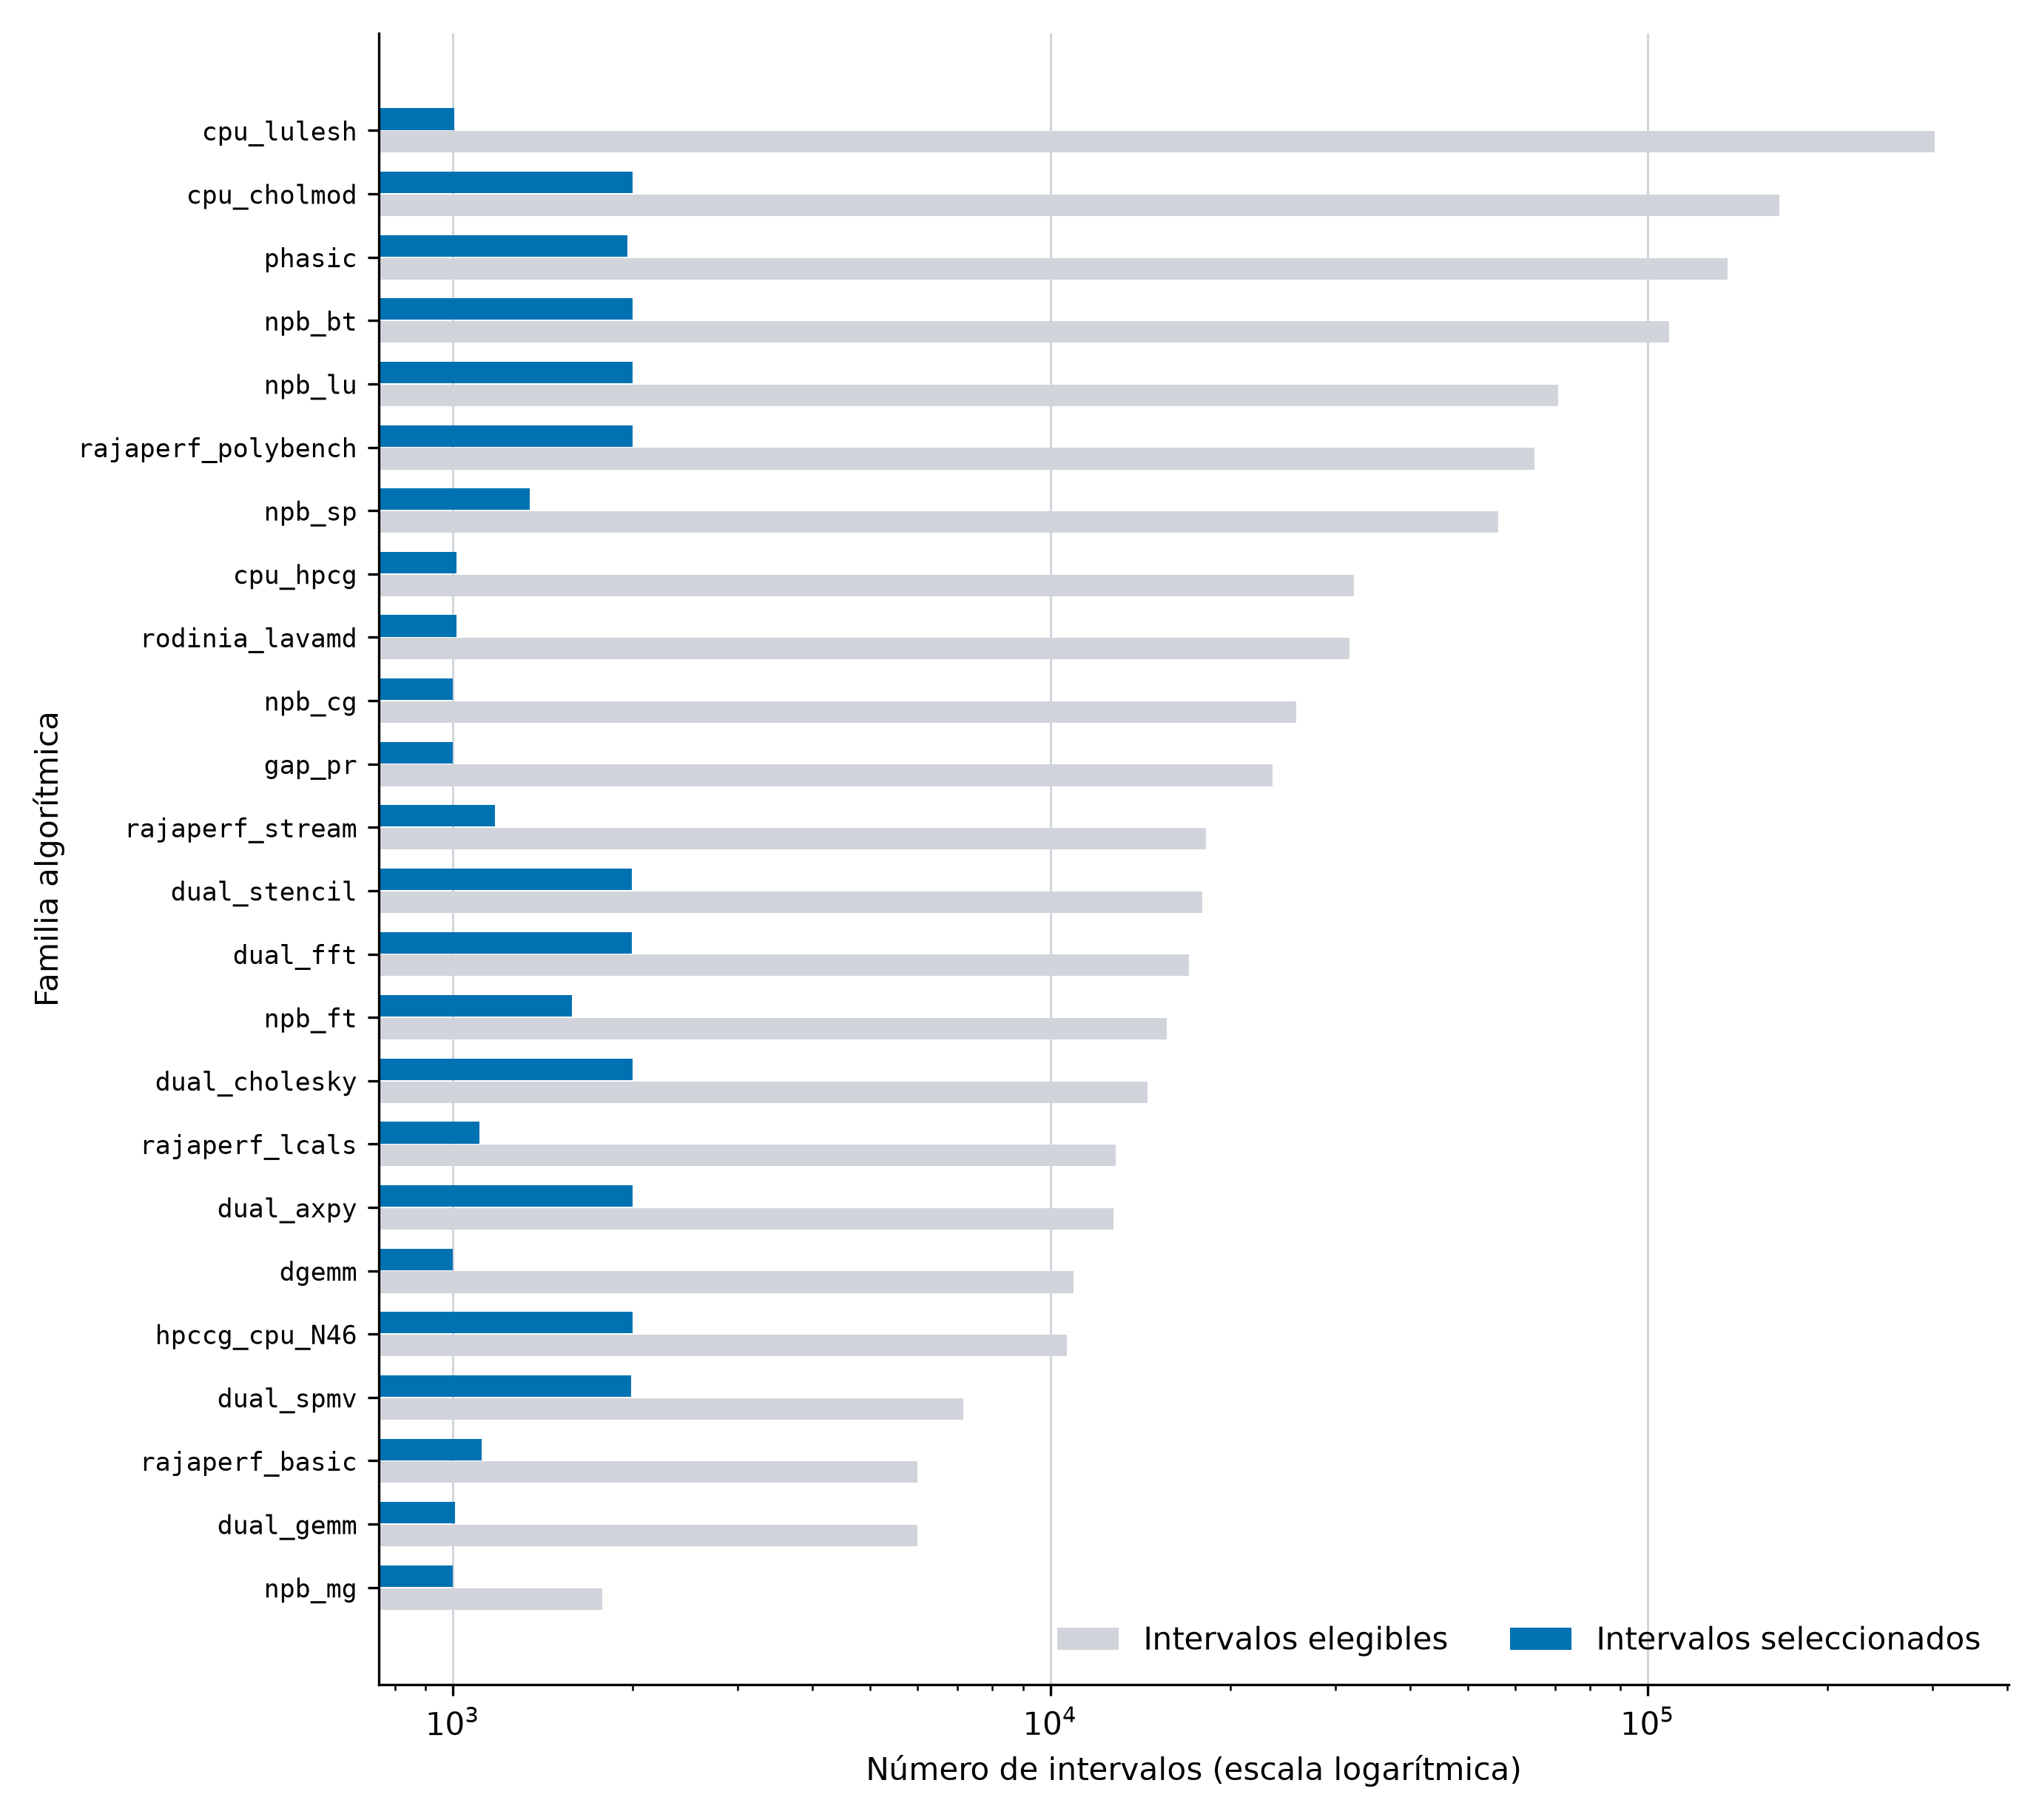
\includegraphics[width=0.92\textwidth]{figuras/fig_cpu_muestreo_familia_20260918.png}
    \caption[Muestreo estratificado del conjunto CPU]{Intervalos elegibles y seleccionados por familia algorítmica. El eje logarítmico permite comparar familias cuyo volumen original difiere en varios órdenes de magnitud. Fuente: elaboración propia.}
    \label{fig:cpu-muestreo-familia}
\end{figure}

\subsubsection{Variables de entrada}
\label{sec:resultados-cpu-entradas}

El modelo usa las seis variables de la Tabla \ref{tab:cpu-features-modelo}: cinco tasas normalizadas calculadas con los contadores del intervalo y la frecuencia física observada.

\begin{table}[H]
\centering
\caption{Variables de entrada del candidato CPU congelado.}
\label{tab:cpu-features-modelo}
\footnotesize
\setlength{\tabcolsep}{3pt}
\begin{tabular}{@{}p{3.6cm}p{4.6cm}p{4.8cm}@{}}
\toprule
\textbf{Variable} & \textbf{Cálculo} & \textbf{Interpretación} \\
\midrule
\texttt{ipc} & $N_{\mathrm{inst}}/N_{\mathrm{cyc}}$ & Trabajo retirado por ciclo \\
\texttt{mpki} & $1000N_{\mathrm{miss}}/N_{\mathrm{inst}}$ & Fallos de caché por millar de instrucciones \\
\texttt{cache\_miss\_rate} & $N_{\mathrm{miss}}/N_{\mathrm{ref}}$ & Fracción de referencias que fallan \\
\texttt{stall\_mem\_ratio} & $N_{\mathrm{stall}}/N_{\mathrm{cyc}}$ & Fracción de ciclos detenidos por memoria \\
\texttt{ips} & $N_{\mathrm{inst}}/\Delta t$ & Tasa de instrucciones del intervalo \\
\texttt{freq\_khz\_observed} & Mediana de las lecturas cubiertas & Frecuencia física observada \\
\bottomrule
\end{tabular}
\end{table}

Quedaron fuera las columnas con las que se calcula la etiqueta (FLOPs, bytes de DRAM, intensidad operacional y \textit{ridge}), porque con ellas el modelo no predeciría la etiqueta sino que la calcularía; los identificadores de kernel, nivel y repetición, que permiten reconocer la carga en lugar de su régimen; las señales de calidad del contador, que describen la adquisición y no la carga; y los deltas crudos, que dependen de la duración del intervalo y son redundantes frente a sus tasas.

La auditoría de correlación (sección \ref{sec:metodologia-correlacion-cpu}) se calculó sobre las doce columnas candidatas, antes de descartar las seis redundantes (Figura \ref{fig:cpu-correlacion-entradas}): el par más alto es 0.89 (Pearson), entre MPKI y las referencias de caché por millar de instrucciones, dos normalizaciones distintas de la misma señal de fallos de caché, y de ese par se retuvo MPKI. Sobre el vector final de seis variables, ningún par supera ya la correlación de 0.85: la correlación absoluta más alta es 0.74 (de Spearman), negativa, entre IPC y la fracción de ciclos detenidos por memoria, y la siguiente es 0.72 entre IPC e IPS. El factor de inflación de la varianza máximo es 5.5 con la correlación de Pearson y 7.3 con la de rangos, ambos de IPC, por debajo del umbral de alerta de 10, de modo que no fue necesario retirar ninguna variable adicional.

\begin{figure}[H]
    \centering
    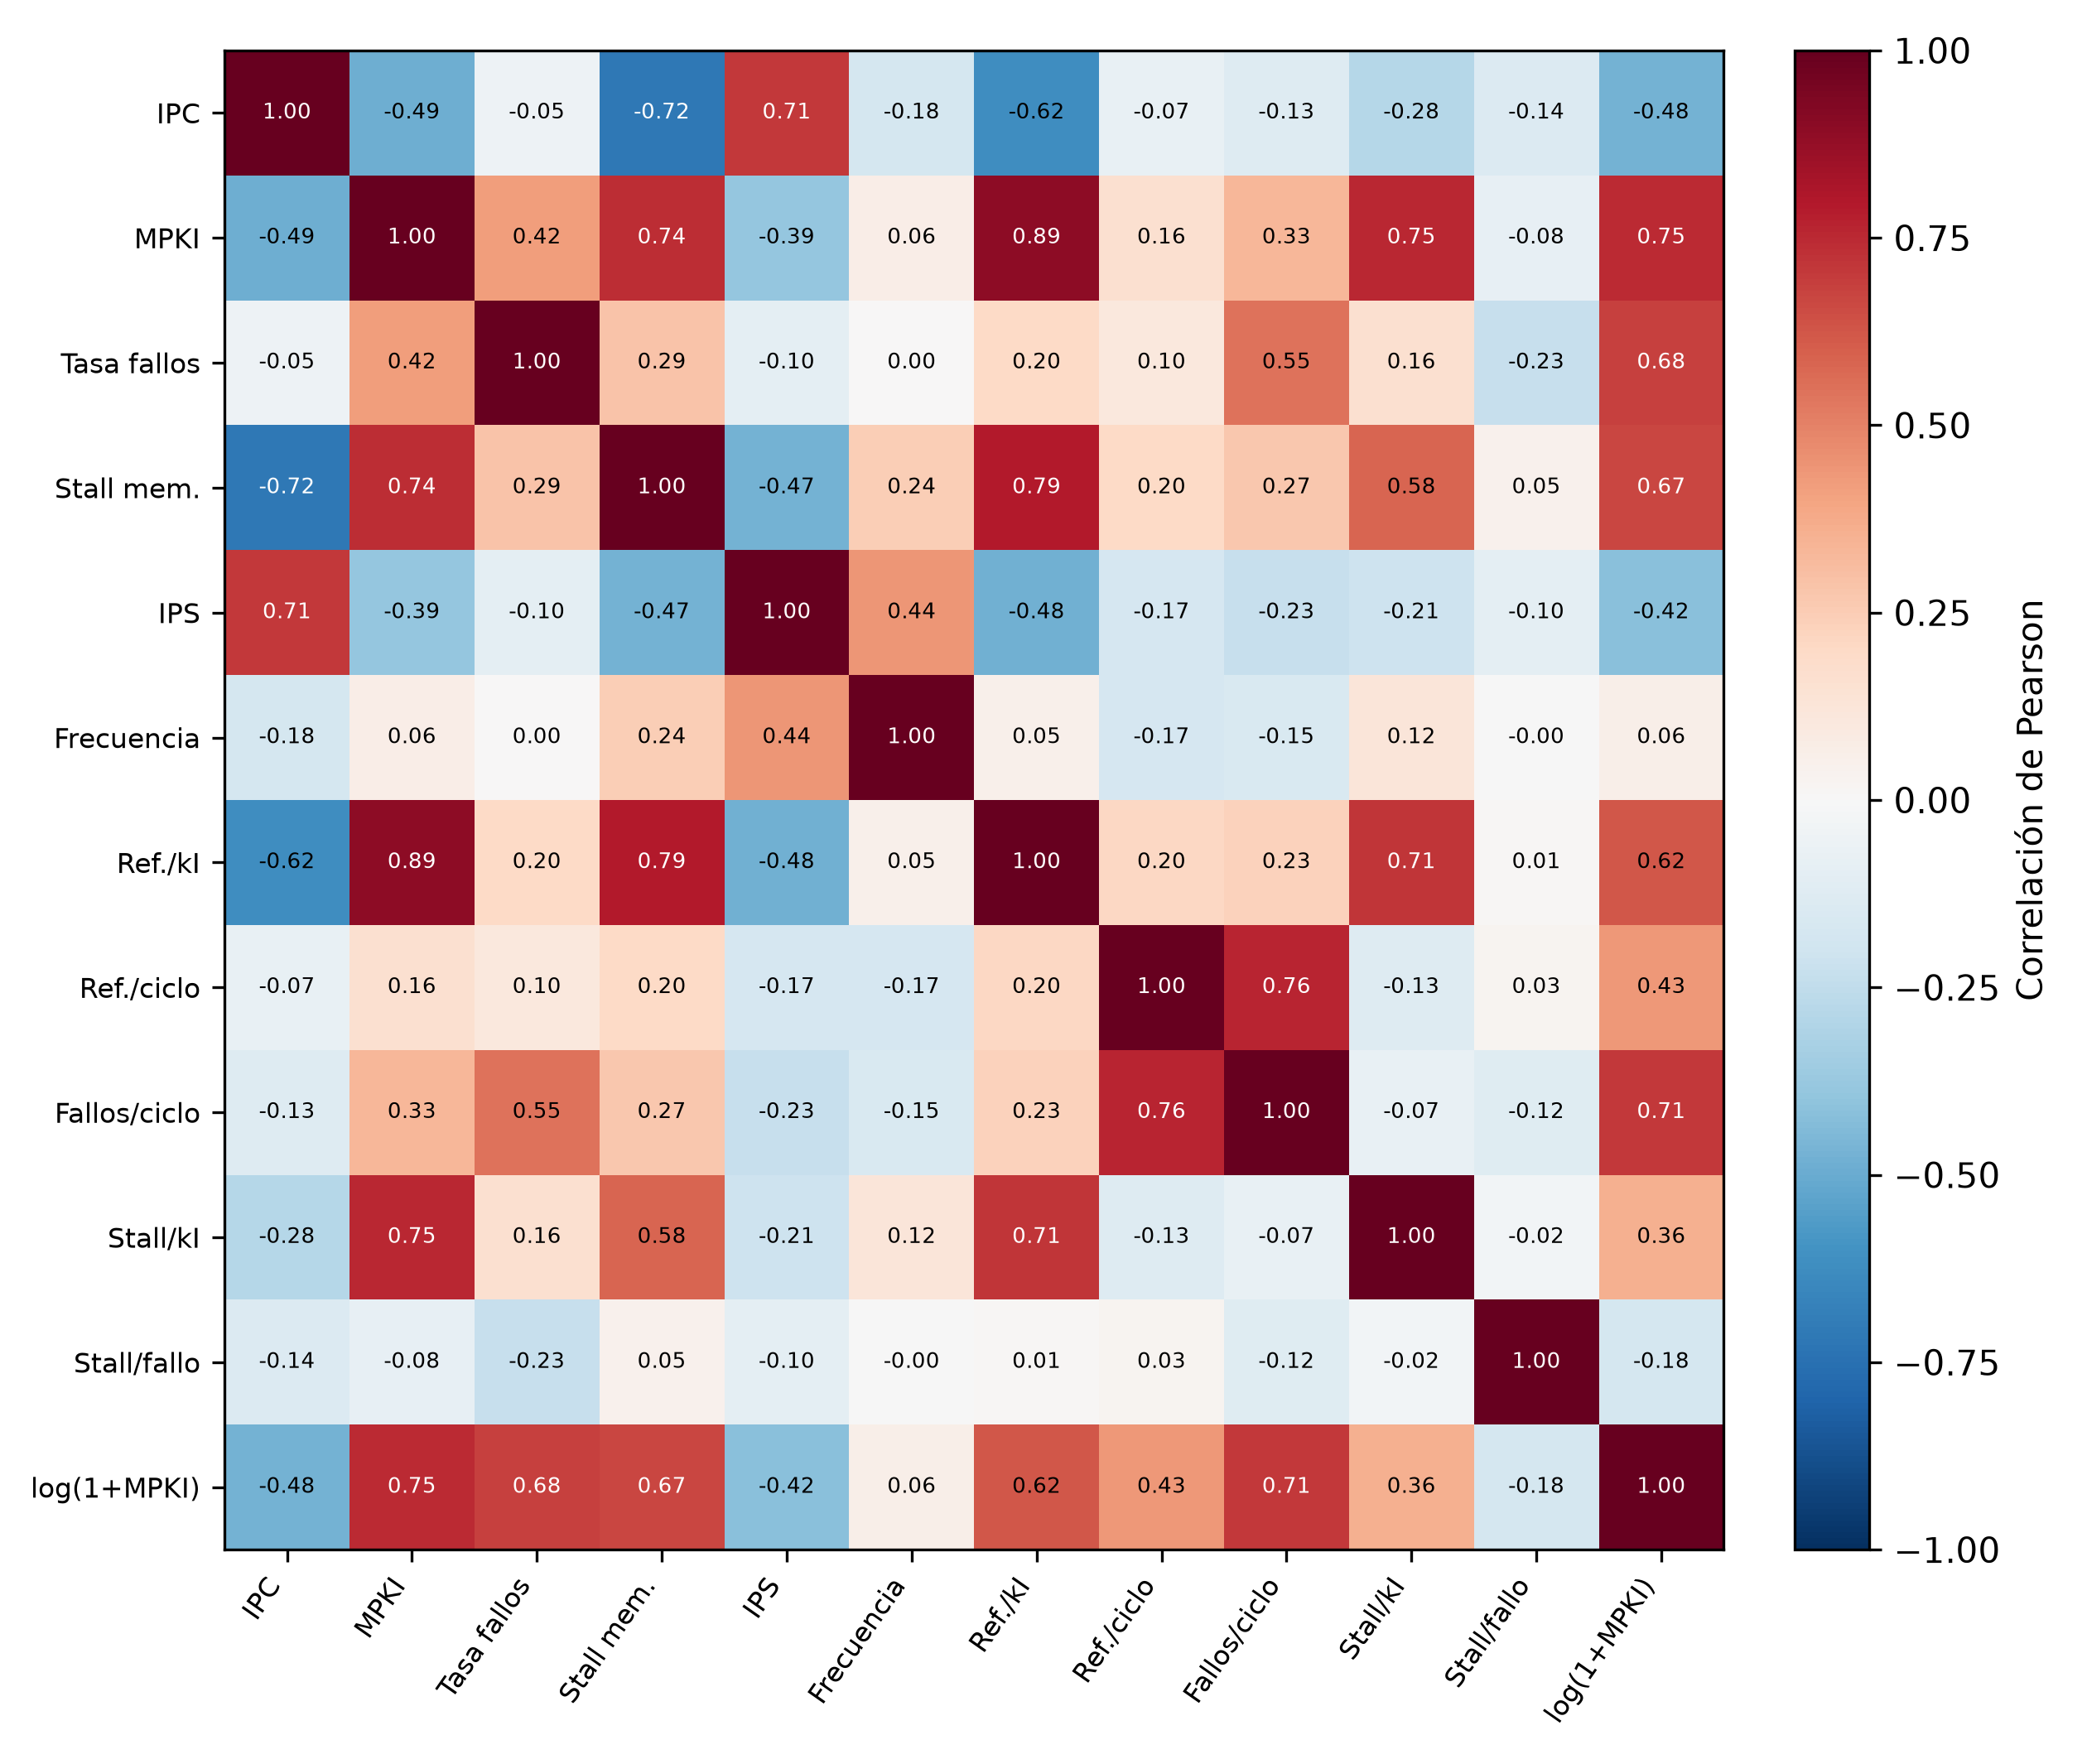
\includegraphics[width=0.72\textwidth]{figuras/fig_cpu_correlacion_entradas_20260918.png}
    \caption[Correlación entre las variables candidatas del clasificador CPU]{Correlación de Pearson entre las doce columnas candidatas, sobre los 1\,309\,755 intervalos elegibles, calculada antes de la selección del vector final de seis variables. Los pares más altos (MPKI con las dos normalizaciones de referencias de caché, 0.89 y 0.75) motivan retirar las columnas derivadas y conservar la medición más directa. Fuente: elaboración propia.}
    \label{fig:cpu-correlacion-entradas}
\end{figure}

Ampliar el vector de seis a doce entradas redundantes cambió la exactitud balanceada de 0.728 a 0.724 (IC95 de la diferencia, $-0.026$ a $+0.011$; Tabla \ref{tab:cpu-variantes-entrada}). Por ello se conservaron seis variables. La redundancia perjudicó más a la regresión logística, sin ofrecer a XGBoost una mejora medible de inferencia o precisión.

La frecuencia observada podría servir de atajo para deducir la etiqueta, porque el \textit{ridge} depende de ella. No ocurre: un modelo que solo la recibe alcanza 0.592, apenas por encima del azar, y retirarla del vector completo reduce el resultado solo 0.008 (IC95 de $-0.018$ a $+0.001$). En términos prácticos, el clasificador es un detector de presión sobre la jerarquía de memoria: al permutarlas, las variables que más deterioran el resultado son MPKI (0.055), la tasa de fallos de caché (0.038) y, en menor medida, la frecuencia (0.021), de modo que las seis columnas contienen bastante menos información que seis variables independientes.




\subsubsection{Selección de modelo e hiperparámetros}
\label{sec:resultados-cpu-modelo}

La Tabla \ref{tab:cpu-comparacion-modelos} y la Figura \ref{fig:cpu-comparacion-modelos} comparan los candidatos con hiperparámetros fijos, cinco semillas y el mismo protocolo LOFO. XGBoost, Extra Trees y Random Forest quedan dentro del mismo intervalo de incertidumbre; la regresión logística rinde menos. Se seleccionó XGBoost por su menor latencia entre los modelos de árboles, más de trece veces inferior a la de los dos bosques.

\begin{table}[H]
\centering
\caption{Comparación de modelos con hiperparámetros fijos, los seis a su vector final de seis variables. La sensibilidad de cada modelo al tamaño del vector de entrada se reporta por separado en la Tabla \ref{tab:cpu-variantes-entrada}. La latencia corresponde a una fila y un hilo, medida en el nodo de destino (paccaA100) con el proceso fijado a cuatro núcleos.}
\label{tab:cpu-comparacion-modelos}
\small
\setlength{\tabcolsep}{3pt}
\begin{tabular}{@{}p{3.9cm}>{\centering\arraybackslash}p{1.7cm}>{\centering\arraybackslash}p{2.8cm}>{\centering\arraybackslash}p{1.5cm}>{\centering\arraybackslash}p{1.8cm}@{}}
\toprule
\textbf{Modelo} & \textbf{Exact. bal.} & \textbf{IC95} & \textbf{F1 macro} & \textbf{Latencia p99} \\
\midrule
Regla mayoritaria & 0.464 & 0.423 a 0.492 & 0.205 & -- \\
Árbol de profundidad 1 & 0.630 & 0.566 a 0.700 & 0.713 & 109~\textmu s \\
Regresión logística & 0.680 & 0.618 a 0.742 & 0.765 & 475~\textmu s \\
Extra Trees & 0.732 & 0.666 a 0.804 & 0.717 & 5477~\textmu s \\
Random Forest & 0.737 & 0.675 a 0.803 & 0.763 & 5453~\textmu s \\
\textbf{XGBoost} & \textbf{0.728} & 0.669 a 0.790 & 0.760 & 404~\textmu s \\
\bottomrule
\end{tabular}
\end{table}

\begin{figure}[H]
    \centering
    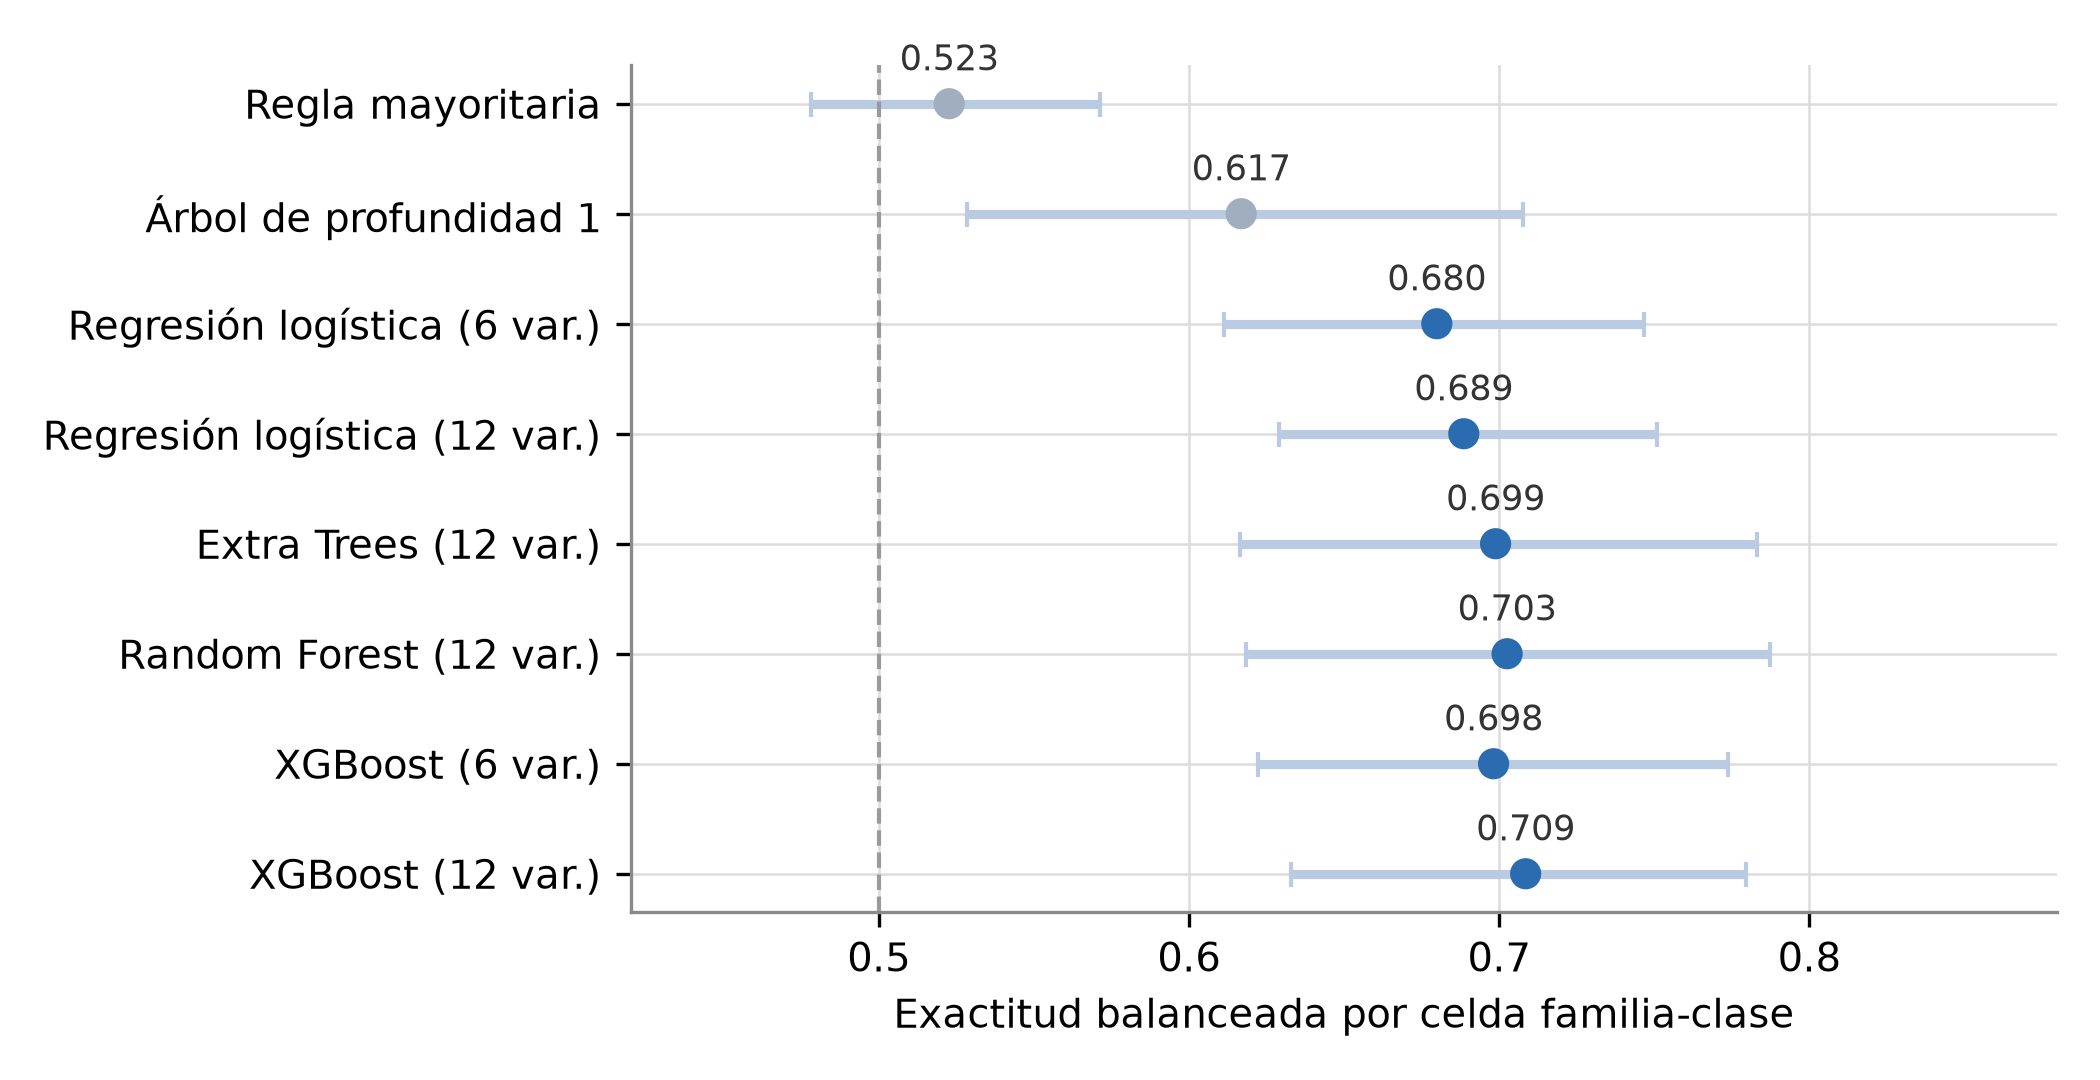
\includegraphics[width=0.92\textwidth]{figuras/fig_cpu_comparacion_modelos_20260919.png}
    \caption[Comparación de modelos del clasificador CPU]{Exactitud balanceada por celda de familia y clase de cada modelo, con intervalo de confianza del 95\% obtenido por remuestreo de las 30 familias. Los intervalos se solapan entre todos los modelos con capacidad suficiente. Fuente: elaboración propia.}
    \label{fig:cpu-comparacion-modelos}
\end{figure}

\paragraph{Búsqueda de hiperparámetros.} Sobre esa base se ejecutó una búsqueda con el muestreador TPE de Optuna \cite{Akiba2019}, anidada dentro de cada pliegue: con la familia retirada apartada, se puntúan las configuraciones con un LOFO interno sobre las 29 restantes, se ajusta la mejor y solo entonces se evalúa la familia retirada. La anidación impide que el resultado se infle por escoger la configuración que mejor se ajusta a la familia reportada. Se evaluaron 15 configuraciones por pliegue para XGBoost y 8 para la regresión logística.

Para XGBoost la búsqueda no mejora de forma distinguible la configuración fija: la diferencia pareada por familia es de $+0.019$, con un intervalo de confianza del 95\% de $-0.007$ a $+0.050$ que incluye el cero (14 familias mejoran, 8 empeoran, de 30). Para la regresión logística el efecto es, en cambio, estadísticamente distinguible de cero (IC95 de $+0.0004$ a $+0.0042$; 5 familias mejoran, 2 empeoran), pero de una magnitud irrelevante, $+0.002$: la búsqueda encuentra una configuración mejor de forma consistente, no por azar, y aun así no cambia en ninguna medida práctica el modelo desplegable. El puntaje interno de cada pliegue se mueve en un rango estrecho (de 0.734 a 0.761) mientras el resultado externo va de 0.487 a 1.000, de modo que el criterio interno no distingue configuraciones buenas de malas para una familia nueva. Por eso se conservó la configuración fija de XGBoost, que además es la más simple de reproducir. La conclusión, coherente con la comparación de modelos y con las variantes del vector de entrada, es que el desempeño no está limitado por la capacidad del modelo ni por el ajuste de sus hiperparámetros.



La configuración congelada es la de la Tabla \ref{tab:cpu-configuracion-final}.


\subsubsection{Métricas de evaluación}
\label{sec:resultados-cpu-metricas}
\label{sec:resultados-cpu-protocolo}

\paragraph{Esquema de evaluación.} Un \emph{pliegue} consiste en retirar una familia completa, ajustar el modelo con las 29 restantes y clasificar después los intervalos de la familia retirada. El procedimiento se repite 30 veces, una por familia, y ningún intervalo de la familia evaluada interviene en el ajuste ni en ninguna decisión de diseño. Responde la pregunta operativa pertinente: si el agente encuentra un algoritmo que nunca vio, ¿acierta su régimen? La alternativa más débil, acertar sobre otra ejecución de un algoritmo ya conocido, da resultados muy distintos con el mismo modelo y los mismos datos (Tabla \ref{tab:cpu-protocolos}): repartir intervalos al azar produce 0.874, porque dos intervalos consecutivos de una misma corrida son casi idénticos y el modelo reconoce la carga en lugar de su régimen. Todas las cifras de este capítulo corresponden a dejar una familia fuera.



\paragraph{Qué es una celda.} Una \emph{celda} es la combinación de una familia algorítmica y una clase de fase; por ejemplo, los intervalos \textit{compute-bound} de \texttt{cpu\_cholmod} forman una celda y sus intervalos \textit{memory-bound} forman otra. El conjunto tiene 56 celdas: 30 familias por dos clases son 60 combinaciones, de las cuales cuatro están vacías porque esa familia nunca presenta esa clase. Cada celda tiene su tamaño, de 5 a más de 300\,000 intervalos, y su fracción de aciertos (Figura \ref{fig:cpu-celdas}).

\begin{figure}[H]
    \centering
    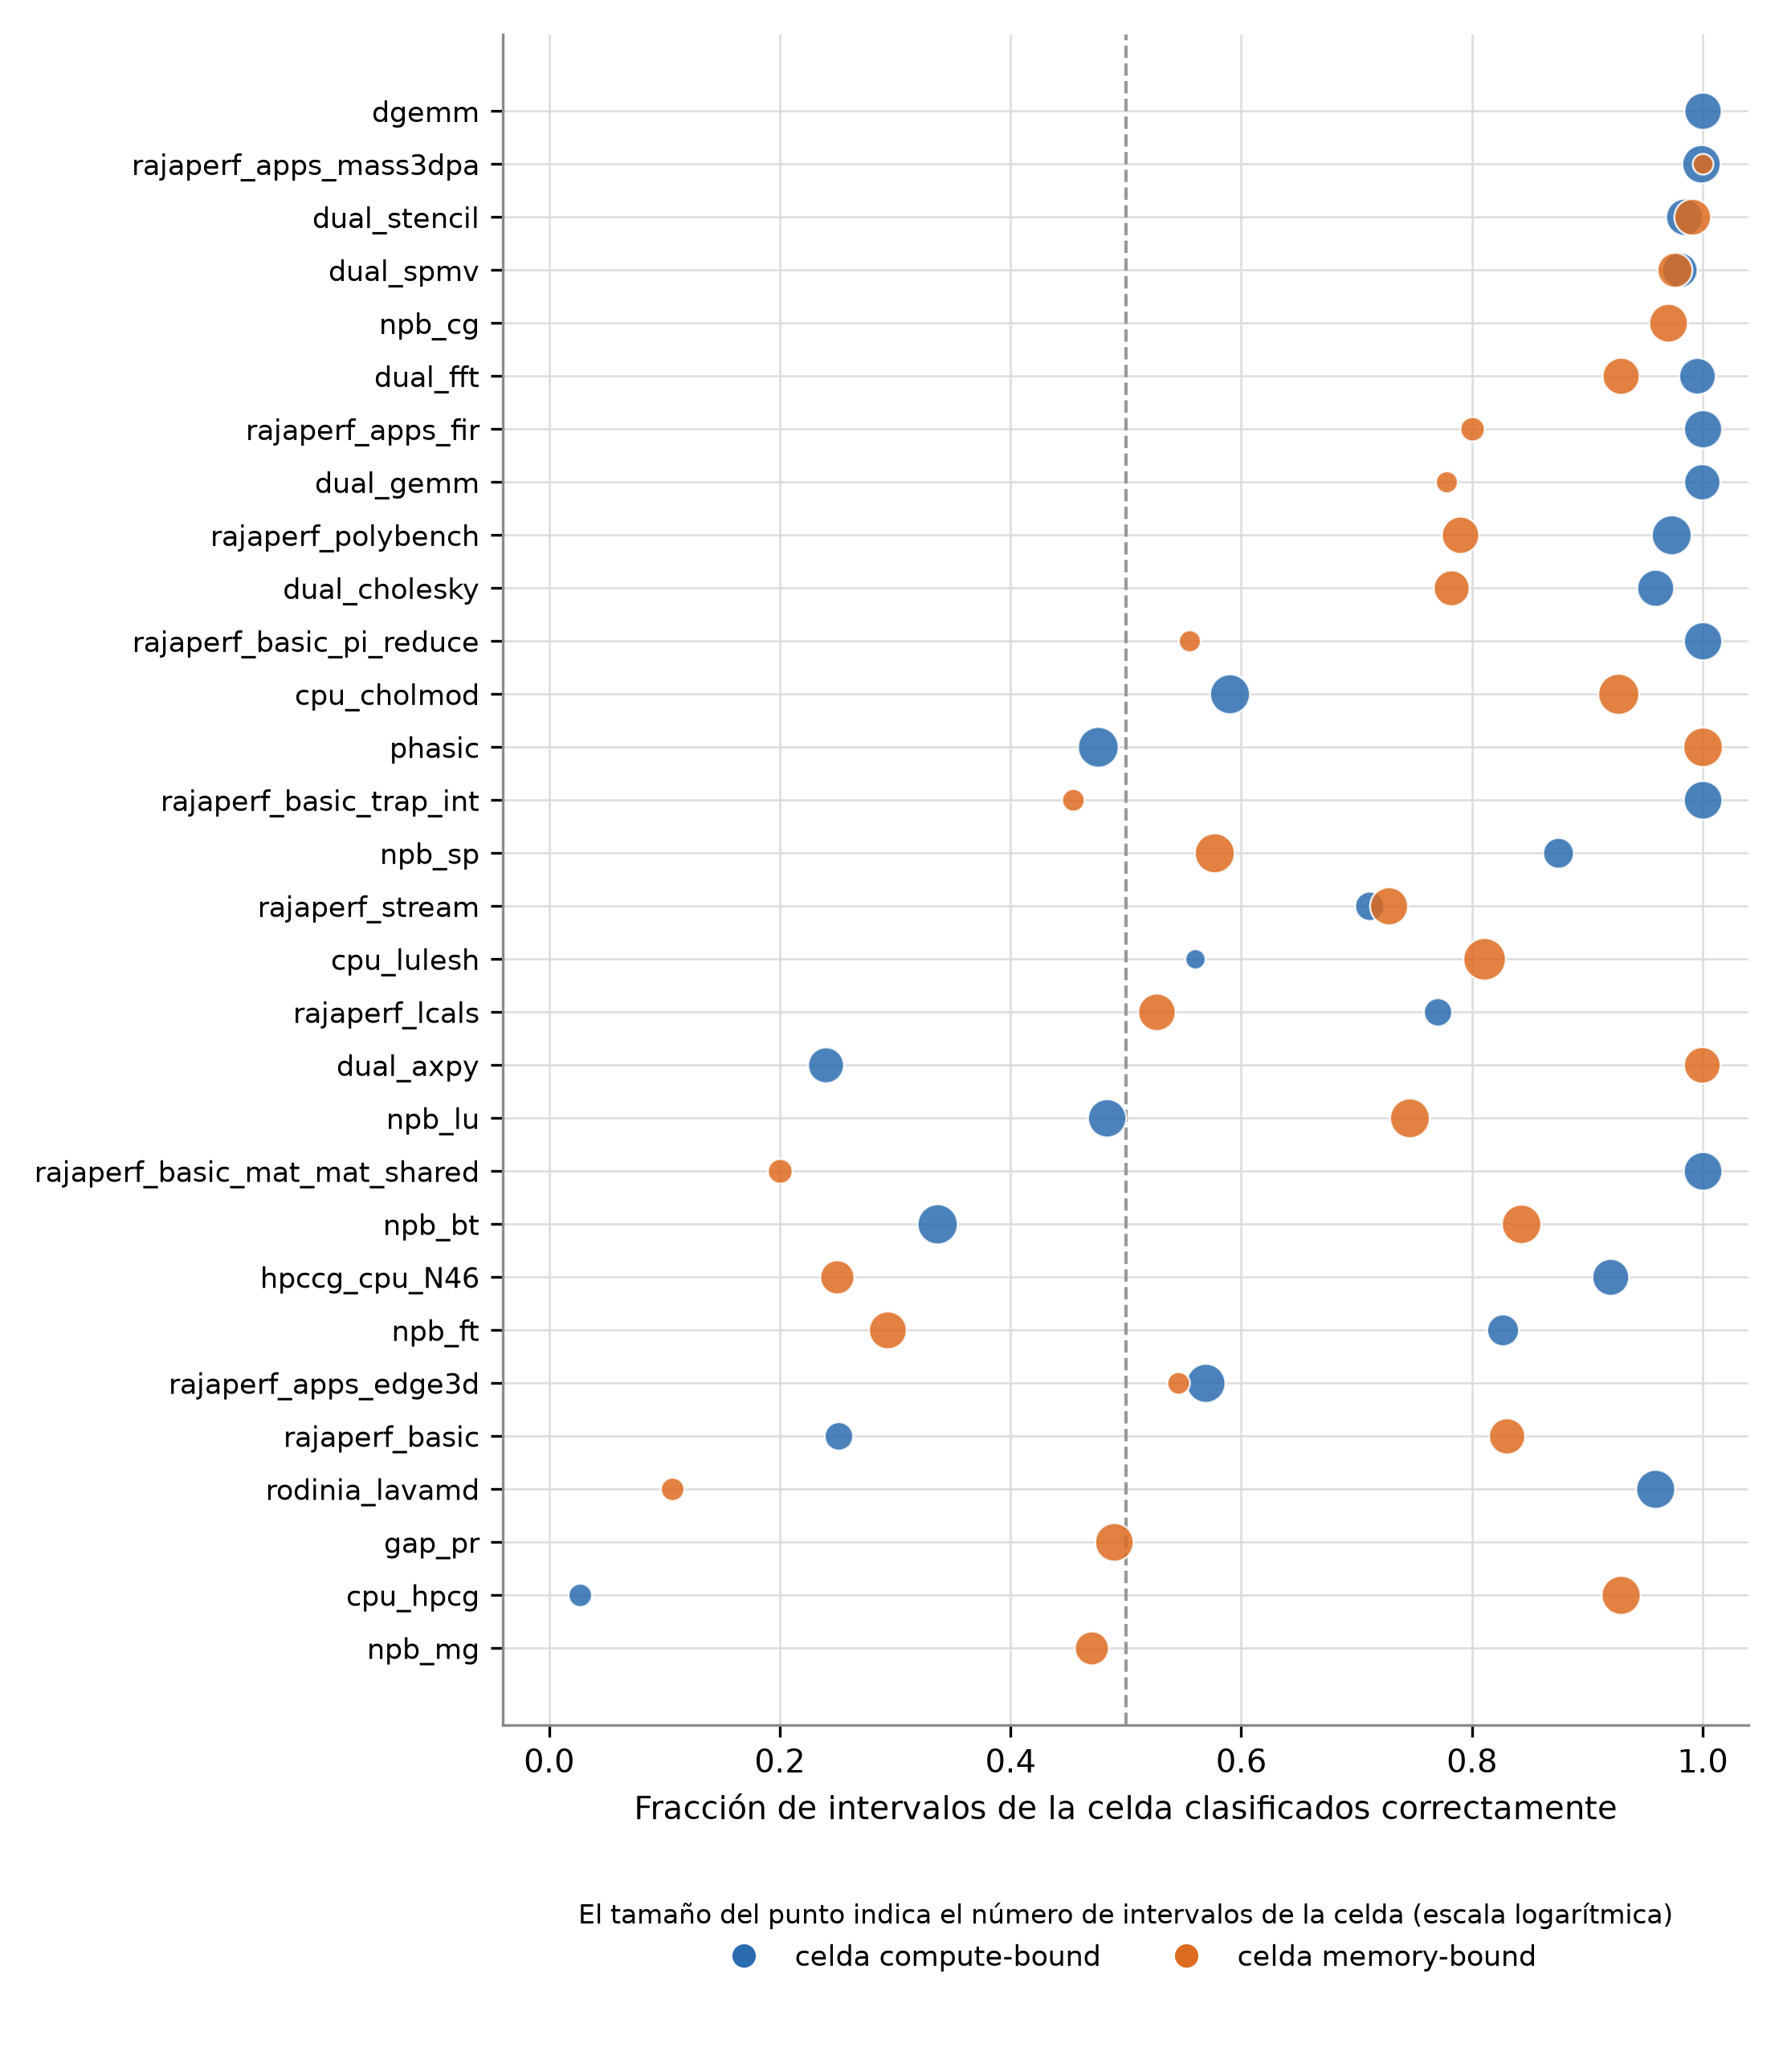
\includegraphics[width=0.94\textwidth]{figuras/fig_cpu_celdas_20260919.png}
    \caption[Acierto del modelo final en cada celda de familia y clase]{Fracción de aciertos del modelo final en cada una de las 56 celdas de familia y clase, con evaluación sobre todos los intervalos de la familia retirada. Las familias con una sola celda son las de una sola clase. Fuente: elaboración propia.}
    \label{fig:cpu-celdas}
\end{figure}

\paragraph{Métricas empleadas.} La Tabla \ref{tab:cpu-metricas-definicion} define las nueve métricas. Para una clase $c$, $\mathrm{VP}_c$ son los intervalos de esa clase correctamente clasificados, $\mathrm{FP}_c$ los de otra clase clasificados como $c$ y $\mathrm{FN}_c$ los de $c$ clasificados como otra clase. Las ocho primeras agrupan todos los intervalos y por ello pesan cada familia según su volumen; la última pesa cada celda por igual.



\paragraph{Por qué la exactitud por celda es la métrica principal.} No depende del volumen, de modo que una corrida larga no decide el resultado; no depende de la proporción entre clases dentro de una familia; y está definida también para las cuatro familias de una sola clase (\texttt{dgemm}, \texttt{gap\_pr}, \texttt{npb\_cg} y \texttt{npb\_mg}), donde el F1 macro calculado dentro de cada familia queda acotado a 0.5 aunque todos sus intervalos se clasifiquen bien. La Tabla \ref{tab:cpu-metricas-valores} reúne todas las métricas del modelo final sin abstención.



La exactitud balanceada clásica (0.760) y la F1 macro agrupada (0.760) coinciden entre sí; la exactitud por celda (0.728) queda unos tres puntos por debajo porque, al pesar cada celda por igual, castiga las celdas de muy pocos intervalos en las que el modelo falla. La exactitud global de 0.769 es la más alta de las tres, pero es la que más depende de la composición del conjunto y no debe leerse como la capacidad del modelo.

\paragraph{Límite de la métrica.} La exactitud por celda asigna el mismo peso a una celda de 5 intervalos que a una de 300\,000. Diez de las 56 celdas tienen menos de 100 intervalos evaluados: suman 128 intervalos y pesan 17.9\% de la métrica; excluirlas la subiría de 0.728 a 0.777. Se conservan porque retirar celdas después de ver que fallan sería seleccionar datos por el resultado, y porque son informativas: muestran que las clases raras dentro de una familia casi pura no se reconocen.

\paragraph{Incertidumbre.} Se informan dos fuentes. La semilla del submuestreo se varió cinco veces. La composición del catálogo se evaluó mediante remuestreo con reemplazo de las 30 familias, con 2000 réplicas. Esta segunda fuente domina y es la que debe usarse al comparar configuraciones: con 30 familias, cualquier diferencia menor que 0.03 es indistinguible del ruido.


\subsubsection{Evaluación del modelo final}
\label{sec:resultados-cpu-final}

Se evaluó el modelo sobre los 1\,309\,755 intervalos elegibles, cada uno clasificado por el modelo del pliegue que no vio su familia, promediando las cinco semillas de muestreo. Si debe emitir siempre una clase, la exactitud balanceada por celda es 0.728, la F1 macro agrupada 0.760 y la exactitud global 0.769. La Tabla \ref{tab:cpu-metricas-clase} desagrega el resultado por clase y la Figura \ref{fig:cpu-matriz-confusion} muestra las matrices de confusión. En el promedio agrupado por intervalo, la sensibilidad de \textit{memory-bound} (0.806) supera en nueve puntos a la de \textit{compute-bound} (0.714); en el promedio por celda de familia y clase la diferencia se invierte y se estrecha (0.700 y 0.759, respectivamente). Ambos promedios describen la misma asimetría: los intervalos \textit{compute-bound} de una familia nueva se parecen más a intervalos \textit{memory-bound} de familias ya vistas que en sentido contrario (sección \ref{sec:resultados-cpu-limite}), y no al desbalance del ajuste, que está corregido por la ponderación.

\begin{figure}[H]
    \centering
    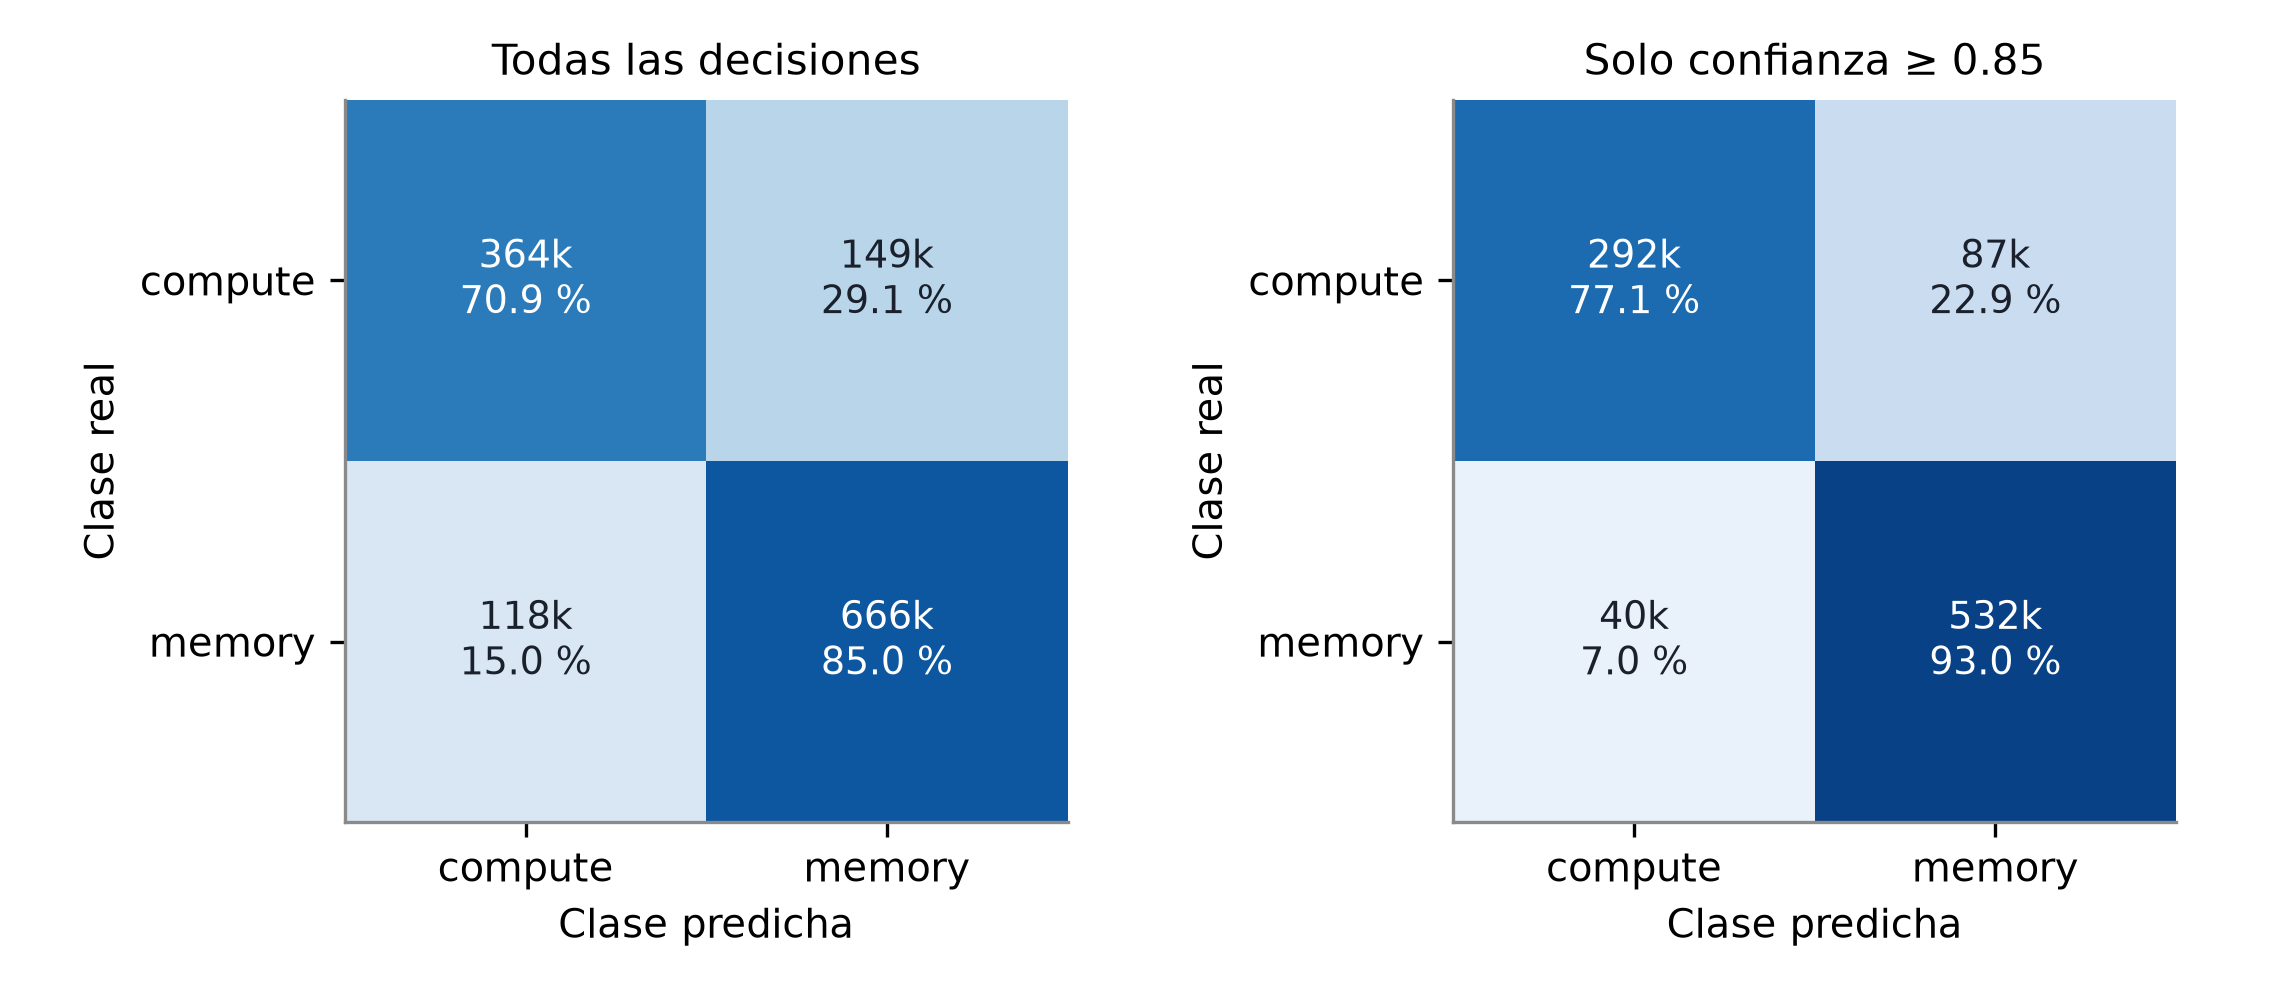
\includegraphics[width=0.94\textwidth]{figuras/fig_cpu_matriz_confusion_20260919.png}
    \caption[Matrices de confusión del clasificador CPU]{Matrices de confusión del modelo final. A la izquierda, cuando se obliga a emitir una clase en todos los intervalos; a la derecha, solo sobre los intervalos con confianza mayor o igual a 0.85. El porcentaje está calculado por fila, es decir, respecto de la clase real. Fuente: elaboración propia.}
    \label{fig:cpu-matriz-confusion}
\end{figure}

El resultado no es uniforme entre familias (Figura \ref{fig:cpu-resultado-familia}). Catorce familias superan 0.9 de exactitud y cinco quedan por debajo de 0.55, con \textit{npb\_ft} en 0.314. Las mejores son las de comportamiento extremo y estable; las peores, aquellas cuyo perfil de contadores coincide con el de familias de la clase contraria.

\begin{figure}[H]
    \centering
    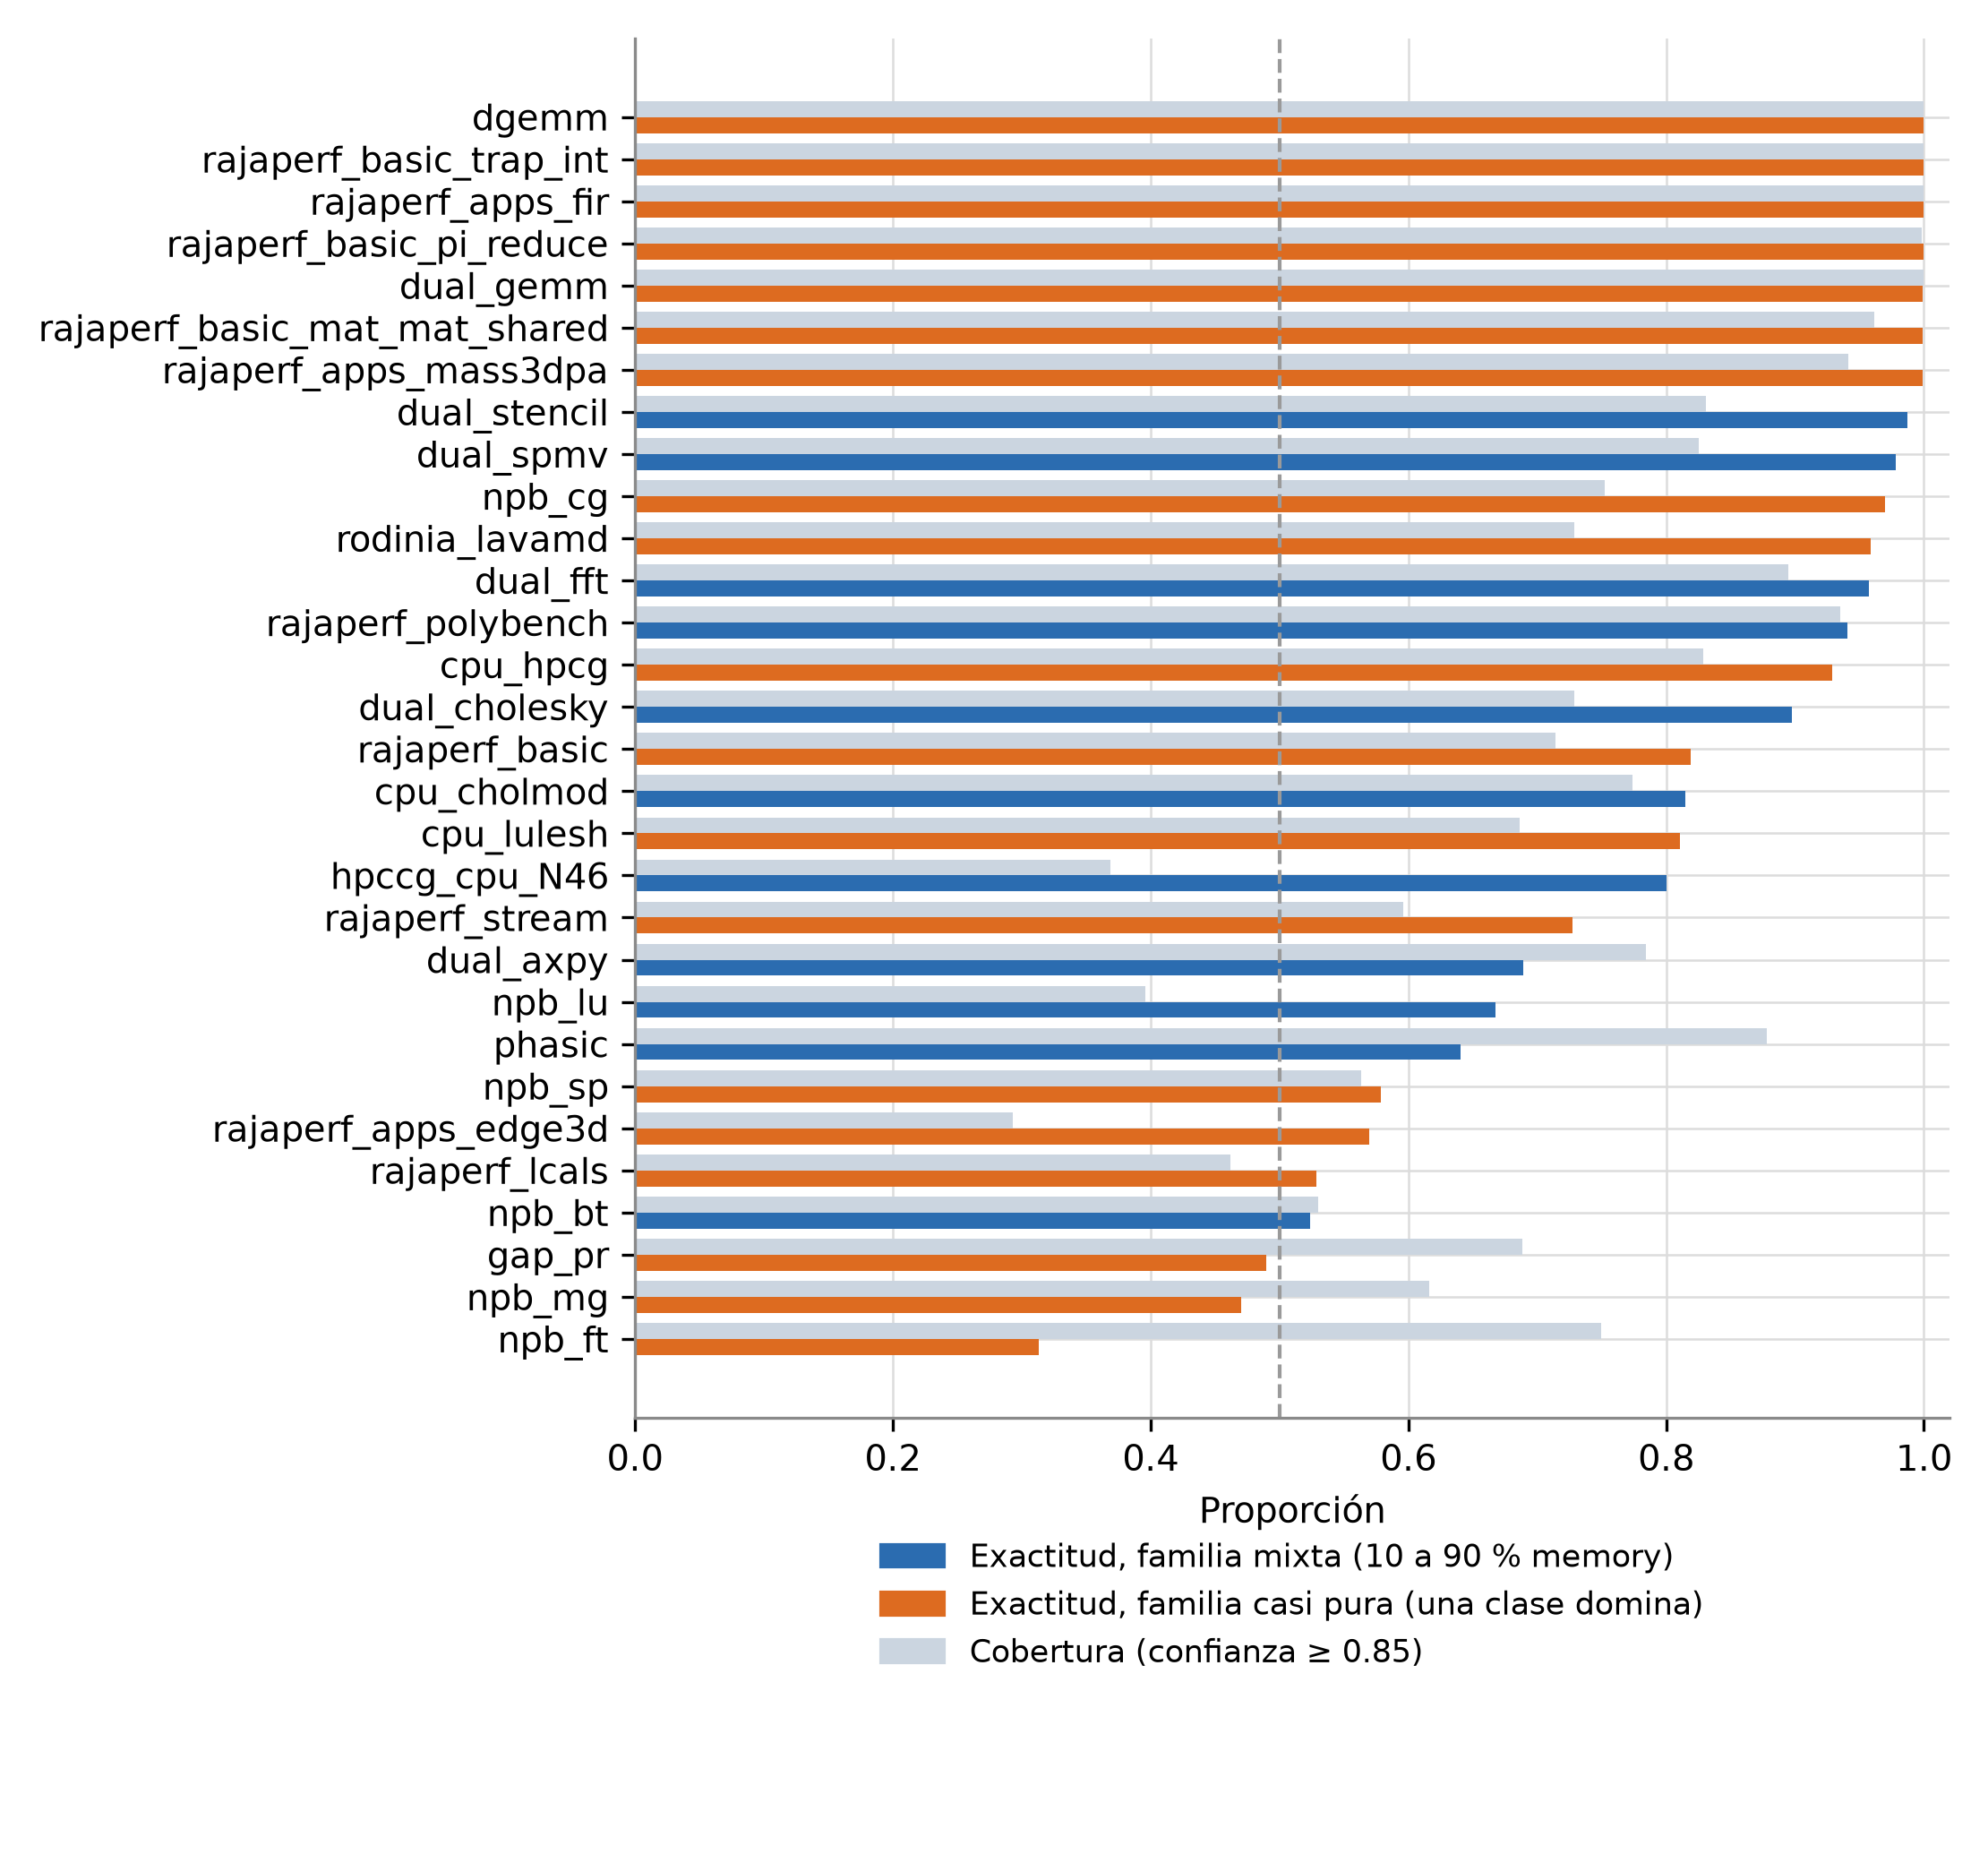
\includegraphics[width=0.94\textwidth]{figuras/fig_cpu_resultado_por_familia_20260919.png}
    \caption[Resultado del clasificador CPU por familia]{Exactitud del modelo final y cobertura de la decisión automática para cada familia retirada. El color distingue las familias mixtas (entre 10 y 90 \% de intervalos memory-bound) de las casi puras. Fuente: elaboración propia.}
    \label{fig:cpu-resultado-familia}
\end{figure}

La Figura \ref{fig:cpu-exactitud-cobertura-frecuencia} resume el desempeño por nivel. Por nivel de frecuencia, en la métrica principal el resultado va de 0.823 en el nivel nativo a 0.657 en F7 (Tabla \ref{tab:cpu-resultado-frecuencia}) y decrece, en general, al bajar el reloj. En los niveles bajos el \textit{ridge} desplaza más intervalos hacia la clase de cómputo (la fracción \textit{memory-bound} baja de 0.71 a 0.54) y la cobertura de la decisión automática cae de 0.85 a 0.64, lo que es consistente con que allí más intervalos quedan cerca de la frontera entre clases. La exactitud global repunta en F8 (0.757, frente a 0.710 en F7), pero ese repunte es casi enteramente un efecto de composición de clases: en la exactitud balanceada por celda, que no depende de cuántos intervalos aporta cada clase, F8 (0.659) queda prácticamente igualado con F7 (0.657) y no rebota. F8 es también el nivel con más intervalos (256\,531, frente a 85\,447--186\,309 en los demás), de modo que su exactitud global pesa más hacia la clase \textit{compute-bound} mayoritaria en ese régimen, que el modelo reconoce mejor a esa frecuencia.




\begin{figure}[H]
    \centering
    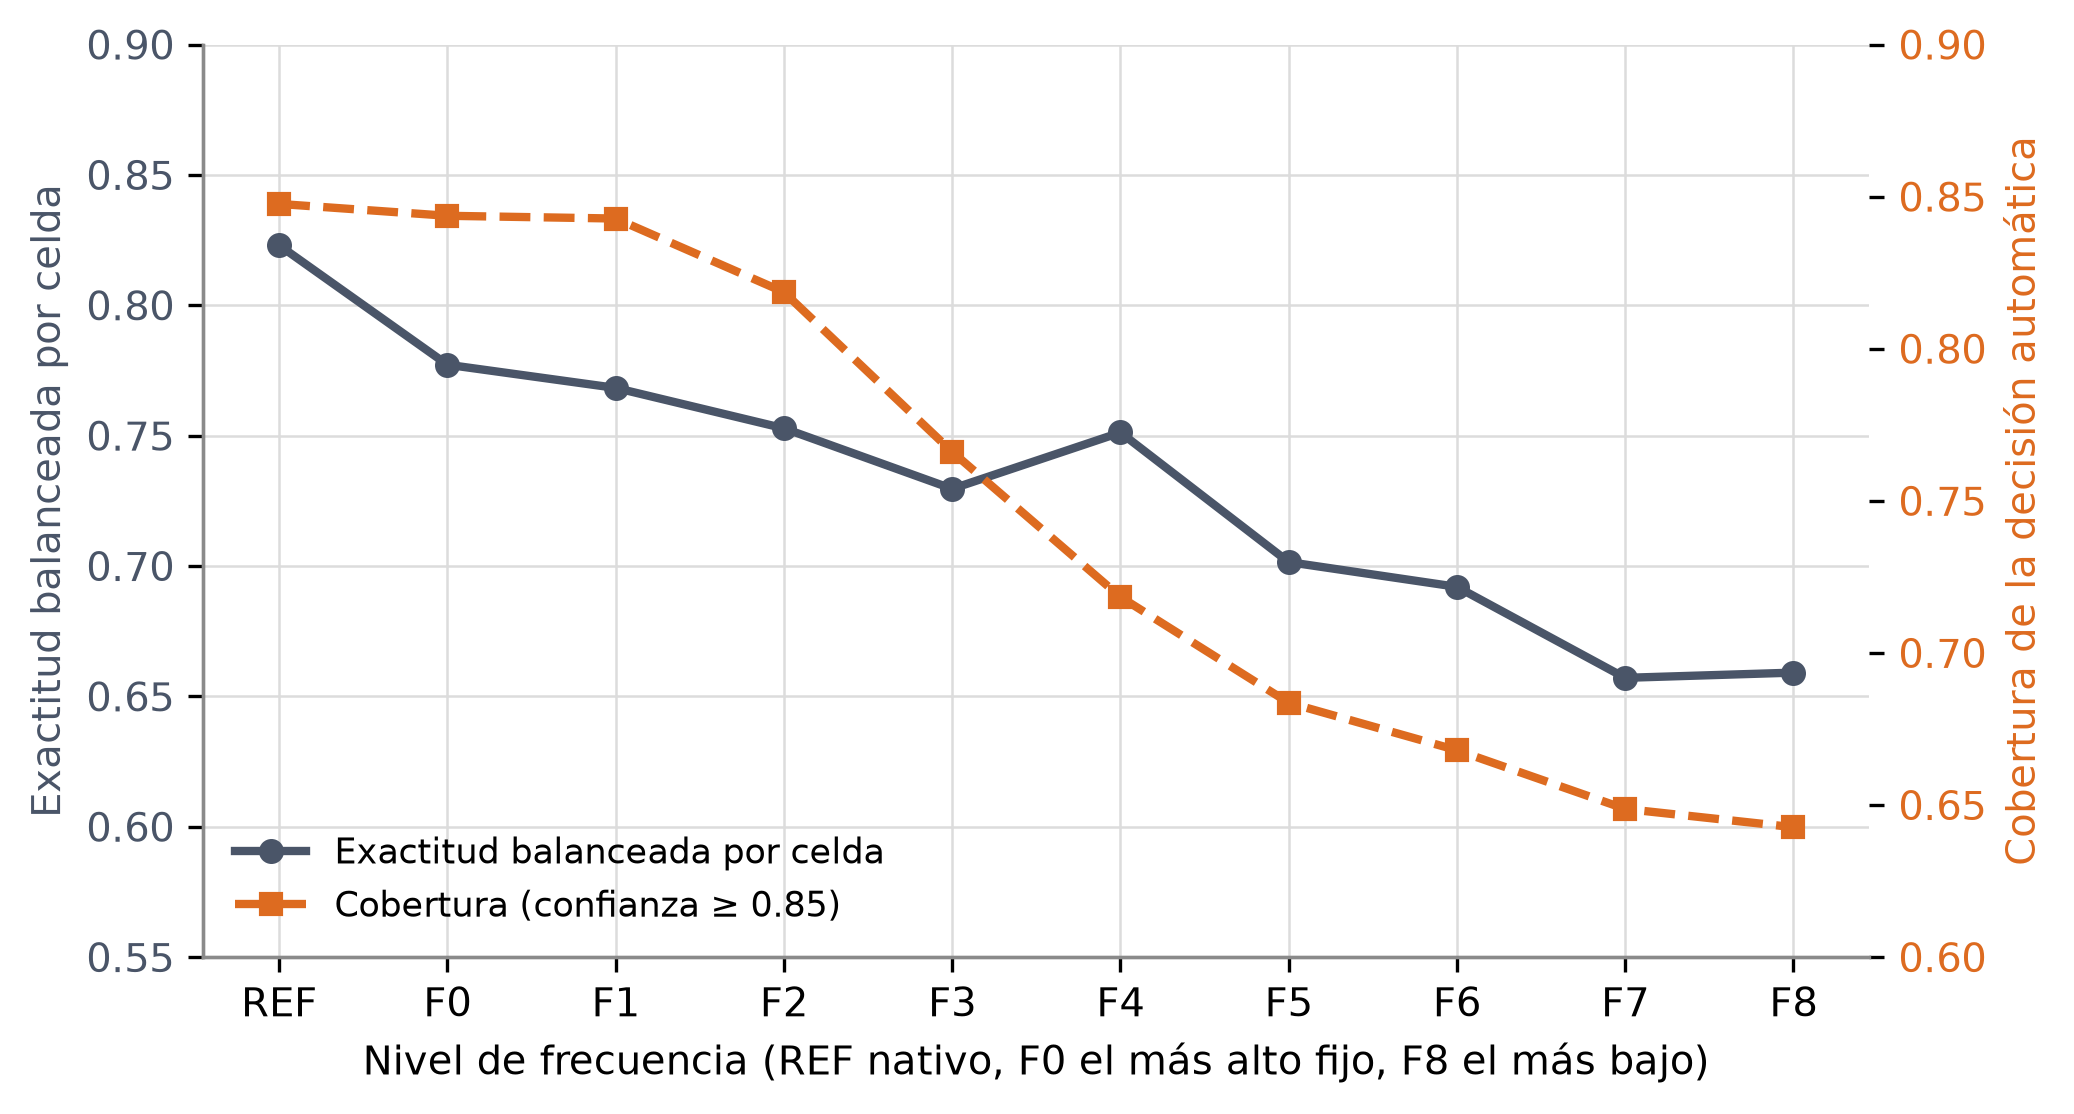
\includegraphics[width=0.78\textwidth]{figuras/fig_cpu_exactitud_cobertura_frecuencia_20260922.png}
    \caption[Exactitud y cobertura del clasificador CPU por nivel de frecuencia]{Exactitud balanceada por celda y cobertura de la decisión automática (confianza $\geq 0.85$) en función del nivel de frecuencia. Ambas caen de forma conjunta al bajar el reloj. Fuente: elaboración propia.}
    \label{fig:cpu-exactitud-cobertura-frecuencia}
\end{figure}

\subsubsection{Decisión selectiva y costo de inferencia}
\label{sec:resultados-cpu-selectiva}

El umbral de abstención CPU se eligió con LOFO interno y un piso de cobertura media por celda de 0.60 (Tabla \ref{tab:cpu-umbral-rejilla}). Aunque la rejilla proponía 0.90, se congeló 0.85: el aumento de exactitud de selección era solo de 0.003 y reducía la cobertura en 6.5 puntos. La evaluación externa del modelo ya congelado se presenta a continuación; el criterio interno y ese resultado no son la misma estimación.

Con el umbral 0.85 ya congelado, evaluado externamente sobre el modelo final, la cobertura es del 72.2\% de los intervalos (75.1\% promediando por familia); el resto recibe \textit{revisar}. Sobre lo que decide, la exactitud balanceada por celda sube de 0.728 a 0.738, la F1 macro agrupada de 0.760 a 0.842 y la sensibilidad de \textit{compute-bound} de 0.714 a 0.762 (Tabla \ref{tab:cpu-selectiva}); la ganancia por celda es modesta y la mayor parte de la mejora se ve en las métricas agrupadas. Abstenerse al azar en una proporción equivalente de intervalos deja la exactitud balanceada en 0.716 y la F1 macro en 0.752, sin mejora, de modo que la ganancia proviene de que la confianza identifica casos difíciles y no de decidir menos.





El límite de la abstención es que la confianza está mal calibrada fuera de la familia de entrenamiento (Figura \ref{fig:cpu-umbral-calibracion}): la confianza media declarada es 0.890 frente a una exactitud observada de 0.764, con un error de calibración esperado de 0.126. Hay familias que fallan \emph{con} confianza alta y a las que el umbral no protege: entre los intervalos con confianza mayor o igual a 0.9, \textit{npb\_ft} acierta el 32\% y \textit{npb\_mg} el 35\%.

\begin{figure}[H]
    \centering
    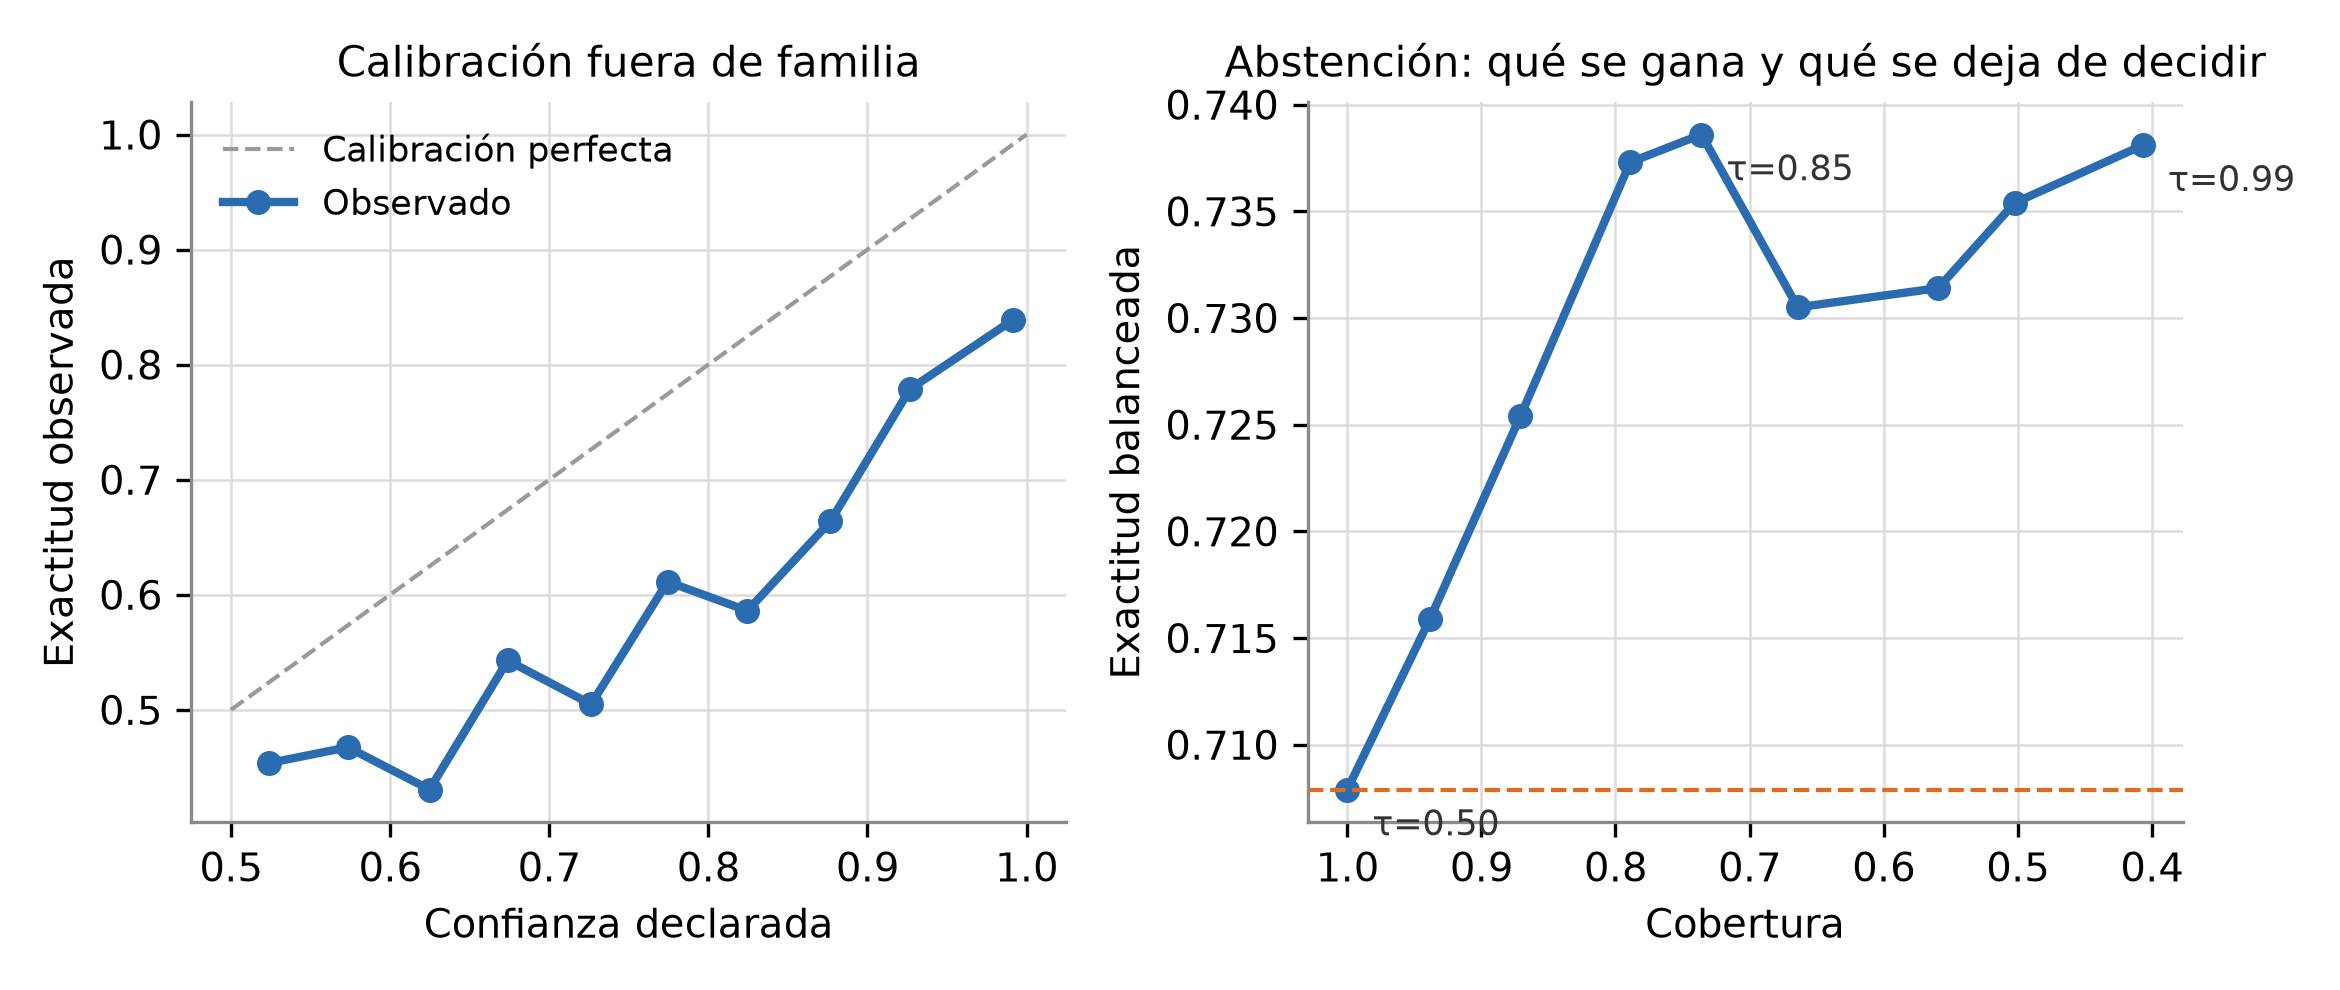
\includegraphics[width=0.96\textwidth]{figuras/fig_cpu_umbral_calibracion_20260919.png}
    \caption[Calibración y compromiso de la abstención en CPU]{A la izquierda, confianza declarada frente a exactitud observada sobre familias no vistas; la curva por debajo de la diagonal indica sobreconfianza. A la derecha, exactitud balanceada alcanzable en función de la cobertura al variar el umbral; ambas curvas usan una sola semilla de muestreo, por lo que sus valores difieren ligeramente de los promedios de cinco semillas de la Tabla \ref{tab:cpu-selectiva}. Fuente: elaboración propia.}
    \label{fig:cpu-umbral-calibracion}
\end{figure}

La salida \textit{revisar} activa una política conservadora: el sistema conserva la frecuencia vigente y espera dos intervalos \textit{uncore} válidos consecutivos antes de aceptar una caracterización física. En cuanto al costo, la inferencia de una fila toma 243~\textmu s de mediana y 404~\textmu s en el percentil 99 para XGBoost, frente a 450 y 475~\textmu s de la regresión logística y 5.3 y 5.5~ms de los bosques, medidos en paccaA100. Estas cifras incluyen la sobrecarga del intérprete de Python y son una cota superior para una implementación integrada en el agente.


\subsubsection{Dónde está el límite del resultado}
\label{sec:resultados-cpu-limite}

Cuatro resultados independientes indican que el límite proviene de la información contenida en los contadores y no del modelo.

El primero es que un clasificador sin ajuste, de 25 vecinos más cercanos sobre cuatro tasas estandarizadas, alcanza 0.684 con el mismo protocolo, y 0.699 si recibe además la frecuencia: queda a menos de 0.045 del modelo final. El segundo es la existencia de perfiles gemelos entre familias de clase opuesta (Figura \ref{fig:cpu-perfiles-gemelos}). El caso más simétrico enfrenta a \textit{gap\_pr}, \textit{memory-bound}, con la fase \textit{compute-bound} de \textit{phasic}: la primera tiene MPKI de 0.82, IPC de 1.11 y tasa de fallos de 0.76; la segunda, MPKI de 0.94, IPC de 0.97 y tasa de fallos de 0.72. El par más cercano en distancia estandarizada, sin embargo, es otro: la celda rara \textit{memory-bound} de \textit{rajaperf\_basic\_mat\_mat\_shared} (apenas el 0.1\% de sus intervalos; la familia es, en conjunto, \textit{compute-bound}) queda a la mitad de distancia de la celda \textit{compute-bound} típica de \textit{rajaperf\_basic\_pi\_reduce}, dos kernels de la misma suite. Ningún modelo que reciba solo esas señales puede separar estos pares, y las tres familias involucradas están entre las de peor resultado.

\begin{figure}[H]
    \centering
    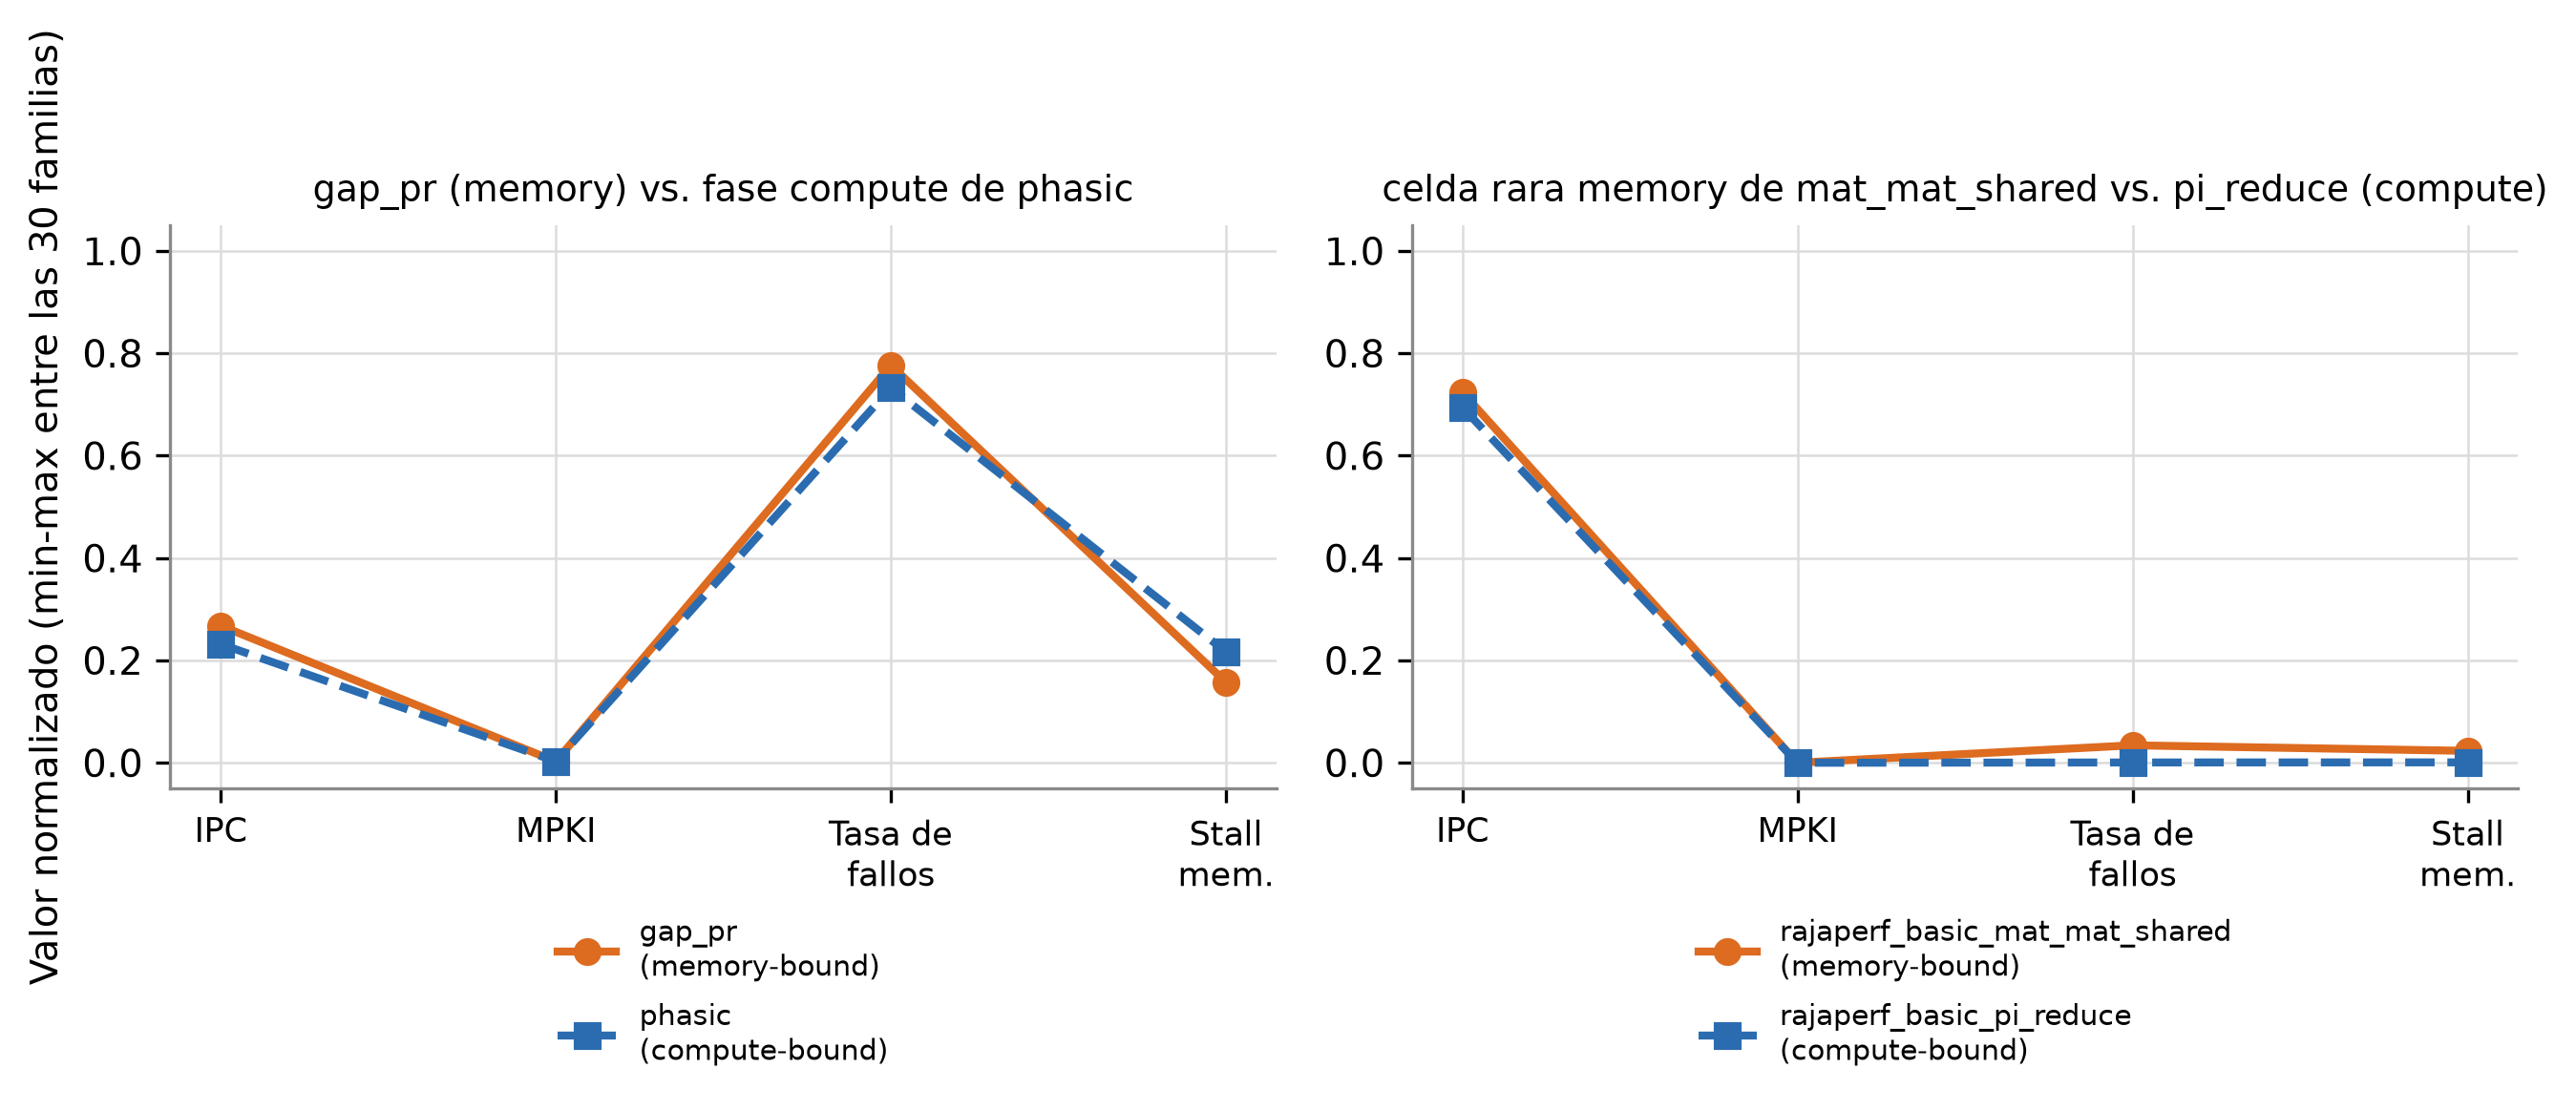
\includegraphics[width=0.96\textwidth]{figuras/fig_cpu_perfiles_gemelos_20260922.png}
    \caption[Perfiles de celdas confusables entre clases opuestas]{Cuatro variables de entrada, normalizadas al rango de las 30 familias, para los dos pares de celdas más confusables entre clases opuestas. Fuente: elaboración propia.}
    \label{fig:cpu-perfiles-gemelos}
\end{figure}

El tercero es la posición respecto del \textit{ridge} (Figura \ref{fig:cpu-margen-ridge}). Los intervalos situados a menos de un factor dos del punto de inflexión son el 12.5\% del total y se clasifican con 0.521 de exactitud, frente a 0.799 en el resto; concentran el 25.3\% de los errores. La ambigüedad cerca de la frontera explica una parte del error, pero tres cuartas partes de los fallos ocurren lejos del \textit{ridge}, donde la etiqueta no es ambigua. Ese error residual, además, no es simétrico alrededor de la frontera: en la franja inmediatamente \textit{compute-bound} (de 0 a 0.5 octavas por encima del \textit{ridge}) la exactitud es 0.318, mientras que en la franja simétrica del lado \textit{memory-bound} (de $-0.5$ a 0 octavas) es 0.766. El modelo no se equivoca por igual a ambos lados de la frontera: cerca de ella, empuja sistemáticamente hacia \textit{memory-bound}, lo mismo que ya se observa en el déficit de sensibilidad de \textit{compute-bound} frente a \textit{memory-bound} (sección \ref{sec:resultados-cpu-final}), y es consistente con los perfiles gemelos del párrafo anterior, en los que la fase \textit{compute-bound} de \textit{phasic} se confunde con \textit{memory-bound}.

\begin{figure}[H]
    \centering
    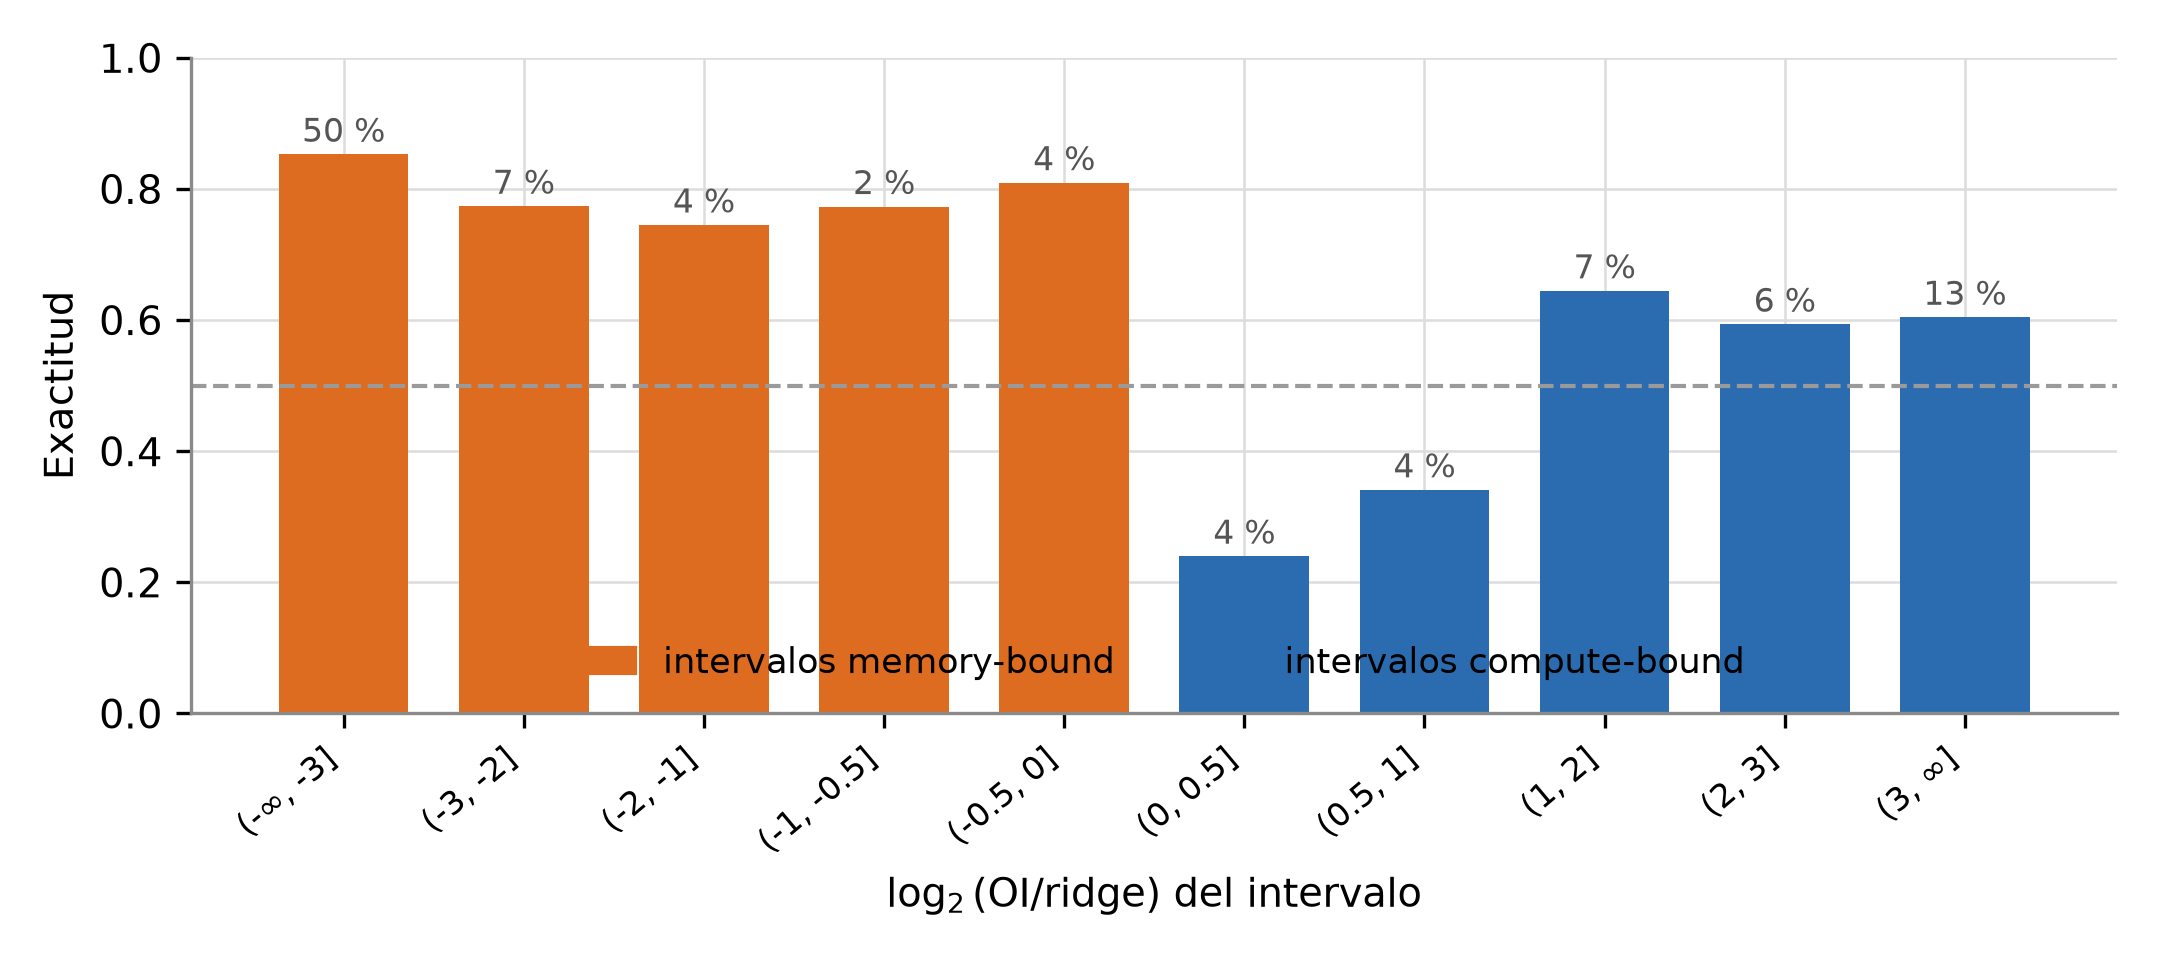
\includegraphics[width=0.94\textwidth]{figuras/fig_cpu_margen_ridge_20260919.png}
    \caption[Exactitud según la distancia al \textit{ridge}]{Exactitud del modelo final por franja de $\log_2(\mathrm{OI}/\mathrm{ridge})$. El porcentaje sobre cada barra indica qué fracción de los intervalos cae en esa franja. Las franjas negativas corresponden a intervalos \textit{memory-bound} y las positivas a \textit{compute-bound}. Fuente: elaboración propia.}
    \label{fig:cpu-margen-ridge}
\end{figure}

El cuarto es la curva de aprendizaje por número de familias (Figura \ref{fig:cpu-curva-aprendizaje}). Al ajustar con subconjuntos de 3 a 23 familias, el resultado sobre la familia retirada sube de 0.615 a 0.718, lo que implica aproximadamente 0.037 de ganancia cada vez que se duplica el catálogo. La diversidad algorítmica gobierna el resultado, y la mejora disponible por esa vía, dentro del alcance de este trabajo, es pequeña.

\begin{figure}[H]
    \centering
    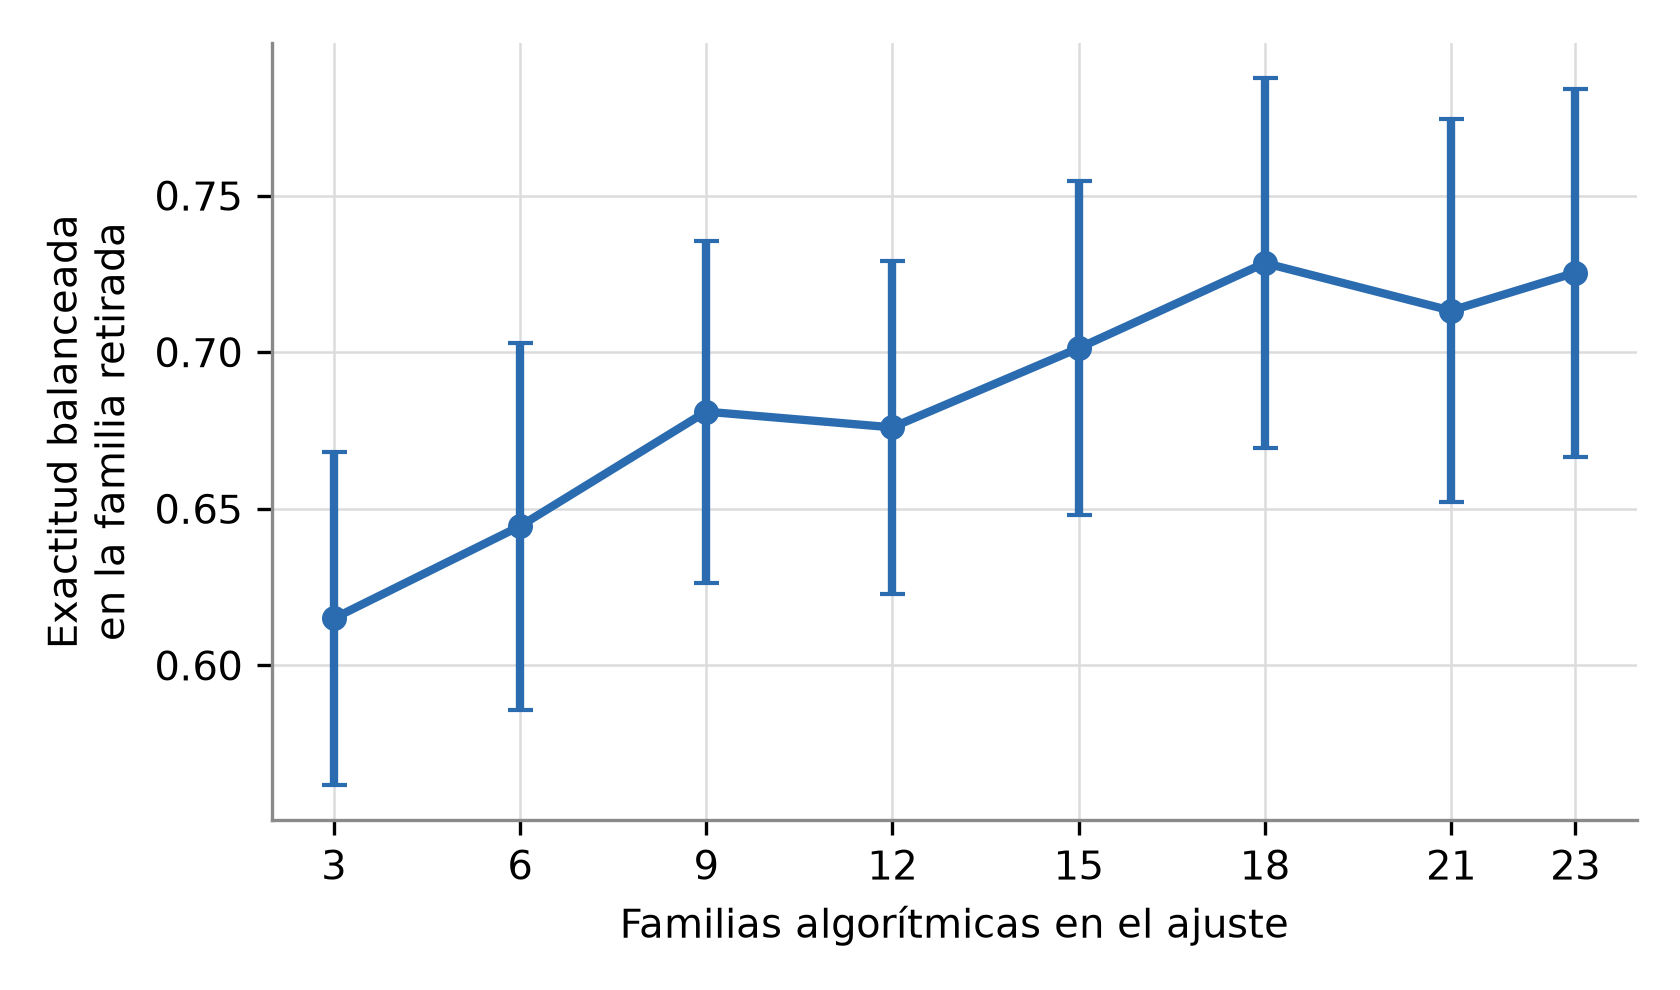
\includegraphics[width=0.72\textwidth]{figuras/fig_cpu_curva_aprendizaje_20260919.png}
    \caption[Curva de aprendizaje por número de familias]{Exactitud balanceada sobre la familia retirada en función del número de familias empleadas en el ajuste. Cada punto promedia las 30 familias retiradas y tres repeticiones de la selección; las barras indican el intervalo de confianza del 95\% entre familias. Fuente: elaboración propia.}
    \label{fig:cpu-curva-aprendizaje}
\end{figure}

Como referencia de límite superior, el mismo modelo con la intensidad operacional medida como entrada adicional alcanza 0.9989, frente a 0.728 sin ella. No es una mejora del modelo, porque la intensidad operacional es la cantidad con la que se define la etiqueta; por eso queda fuera del vector de entrada y solo muestra que la brecha entre 0.728 y 1 es información que los contadores de rendimiento no transportan.


\subsubsection{Síntesis del clasificador CPU}
\label{sec:resultados-cpu-sintesis}

El modelo es un XGBoost de 100 árboles y profundidad 6 que recibe seis variables derivadas de los contadores de rendimiento (cinco tasas normalizadas y la frecuencia observada), se ajusta dando el mismo peso total a cada combinación de familia y clase, y responde \textit{compute-bound}, \textit{memory-bound} o \textit{revisar} según su confianza supere o no 0.85. Ante un algoritmo que nunca vio clasifica correctamente el 72.8\% de los casos en la métrica balanceada por celda, cifra que sube a 73.8\% si se le permite abstenerse en el 27.8\% de los intervalos. La referencia sin capacidad de discriminar queda en 0.464 y la inferencia cuesta 404~\textmu s en el peor percentil medido.

Tres decisiones de diseño resultaron indiferentes: el algoritmo de aprendizaje, el tamaño del vector de entrada y los hiperparámetros. Elegir Random Forest en lugar de XGBoost, usar seis variables en lugar de doce o ajustar los hiperparámetros mueve el resultado menos de lo que lo mueve cambiar de conjunto de familias. Lo que gobierna el resultado es la diversidad del catálogo frente a la información de los contadores: la etiqueta se define por FLOPs sobre bytes de DRAM, mientras que el modelo observa fallos de caché, ciclos detenidos e instrucciones retiradas, que no guardan una relación fija con esa razón cuando cambia el algoritmo.

Quedan tres líneas de trabajo, fuera del alcance de esta fase. La primera es dar contenido a la salida \textit{revisar}: en lugar de solo esperar, el agente de la Fase 3 podría medir la etiqueta física de una fracción mínima de intervalos de la carga en ejecución; esa capacidad se diseña y evalúa allí, con su propio método y protocolo, y no se anticipa aquí con una cifra suelta. La segunda es ampliar el catálogo con familias elegidas por su distancia a los perfiles ya cubiertos y reservar algunas para una prueba externa sellada; las seis familias de cómputo denso de RAJAPerf provienen de una misma suite, de modo que su independencia entre sí es menor que la de familias de suites distintas. La tercera es medir la latencia dentro del agente y no en el intérprete.

Los datos, las figuras y las tablas de esta sección se reproducen con \path{fase2_clasificador/analysis/cpu_quality_report.py} y \path{docs/libro/scripts/generar_figuras_modelo_cpu.py}, sobre los artefactos de \path{docs/libro/datos/cpu_calidad_30fam}.

\subsection{Política de frecuencia por clase en CPU}
\label{sec:resultados-cpu-politica}

La política CPU compara la mediana de tres repeticiones por kernel y frecuencia con su propio REF. Un nivel debía mejorar el EDP agregado con evidencia estadística y al menos 1\% para adoptarse; ese mínimo se fijó después de ver el resultado y se declara como tal. Se excluyeron las variantes \textit{phasic}, cuyo trabajo cambia con la frecuencia pese a su duración fija. La Tabla \ref{tab:cpu-politica-ic} resume la decisión; la rejilla completa está en la Tabla \ref{tab:cpu-politica-detalle} del anexo.

La política resultante es \textit{no actuar} en ambas clases (Tabla \ref{tab:cpu-politica-ic} y Figura \ref{fig:cpu-politica-forest}). La Figura \ref{fig:cpu-energia-relativa} separa la energía y el tiempo que producen ese resultado. En cómputo, F0 mejora 0.56\% frente a REF, menos que el efecto mínimo relevante de 1\%; todos los niveles inferiores empeoran el EDP. En memoria tampoco hay ganancia agregada a menor reloj. Algunos kernels STREAM presentan ahorros puntuales entre 4 y 11\% en su mejor nivel, pero el signo y la magnitud varían entre niveles y repeticiones; no justifican una regla común.

\begin{table}[H]
\centering
\caption{Síntesis de la política CPU. Las ganancias son de EDP frente a REF; la rejilla completa se conserva en la Tabla \ref{tab:cpu-politica-detalle} del Anexo \ref{anexo:resultados-complementarios}.}
\label{tab:cpu-politica-ic}
\small
\begin{tabular}{@{}p{2.5cm}p{7.7cm}p{3.1cm}@{}}
\toprule
\textbf{Clase} & \textbf{Evidencia decisiva} & \textbf{Política} \\
\midrule
Cómputo & F0: $+0.56\%$ (IC95 $[0.27;1.38]$), por debajo del mínimo relevante de $1\%$; F1--F8 empeoran & No actuar \\
Memoria & F1: $-5.4\%$ (IC95 $[-6.8;-3.4]$); ningún nivel bajo mejora el agregado & No actuar \\
\bottomrule
\end{tabular}
\end{table}

\begin{figure}[H]
    \centering
    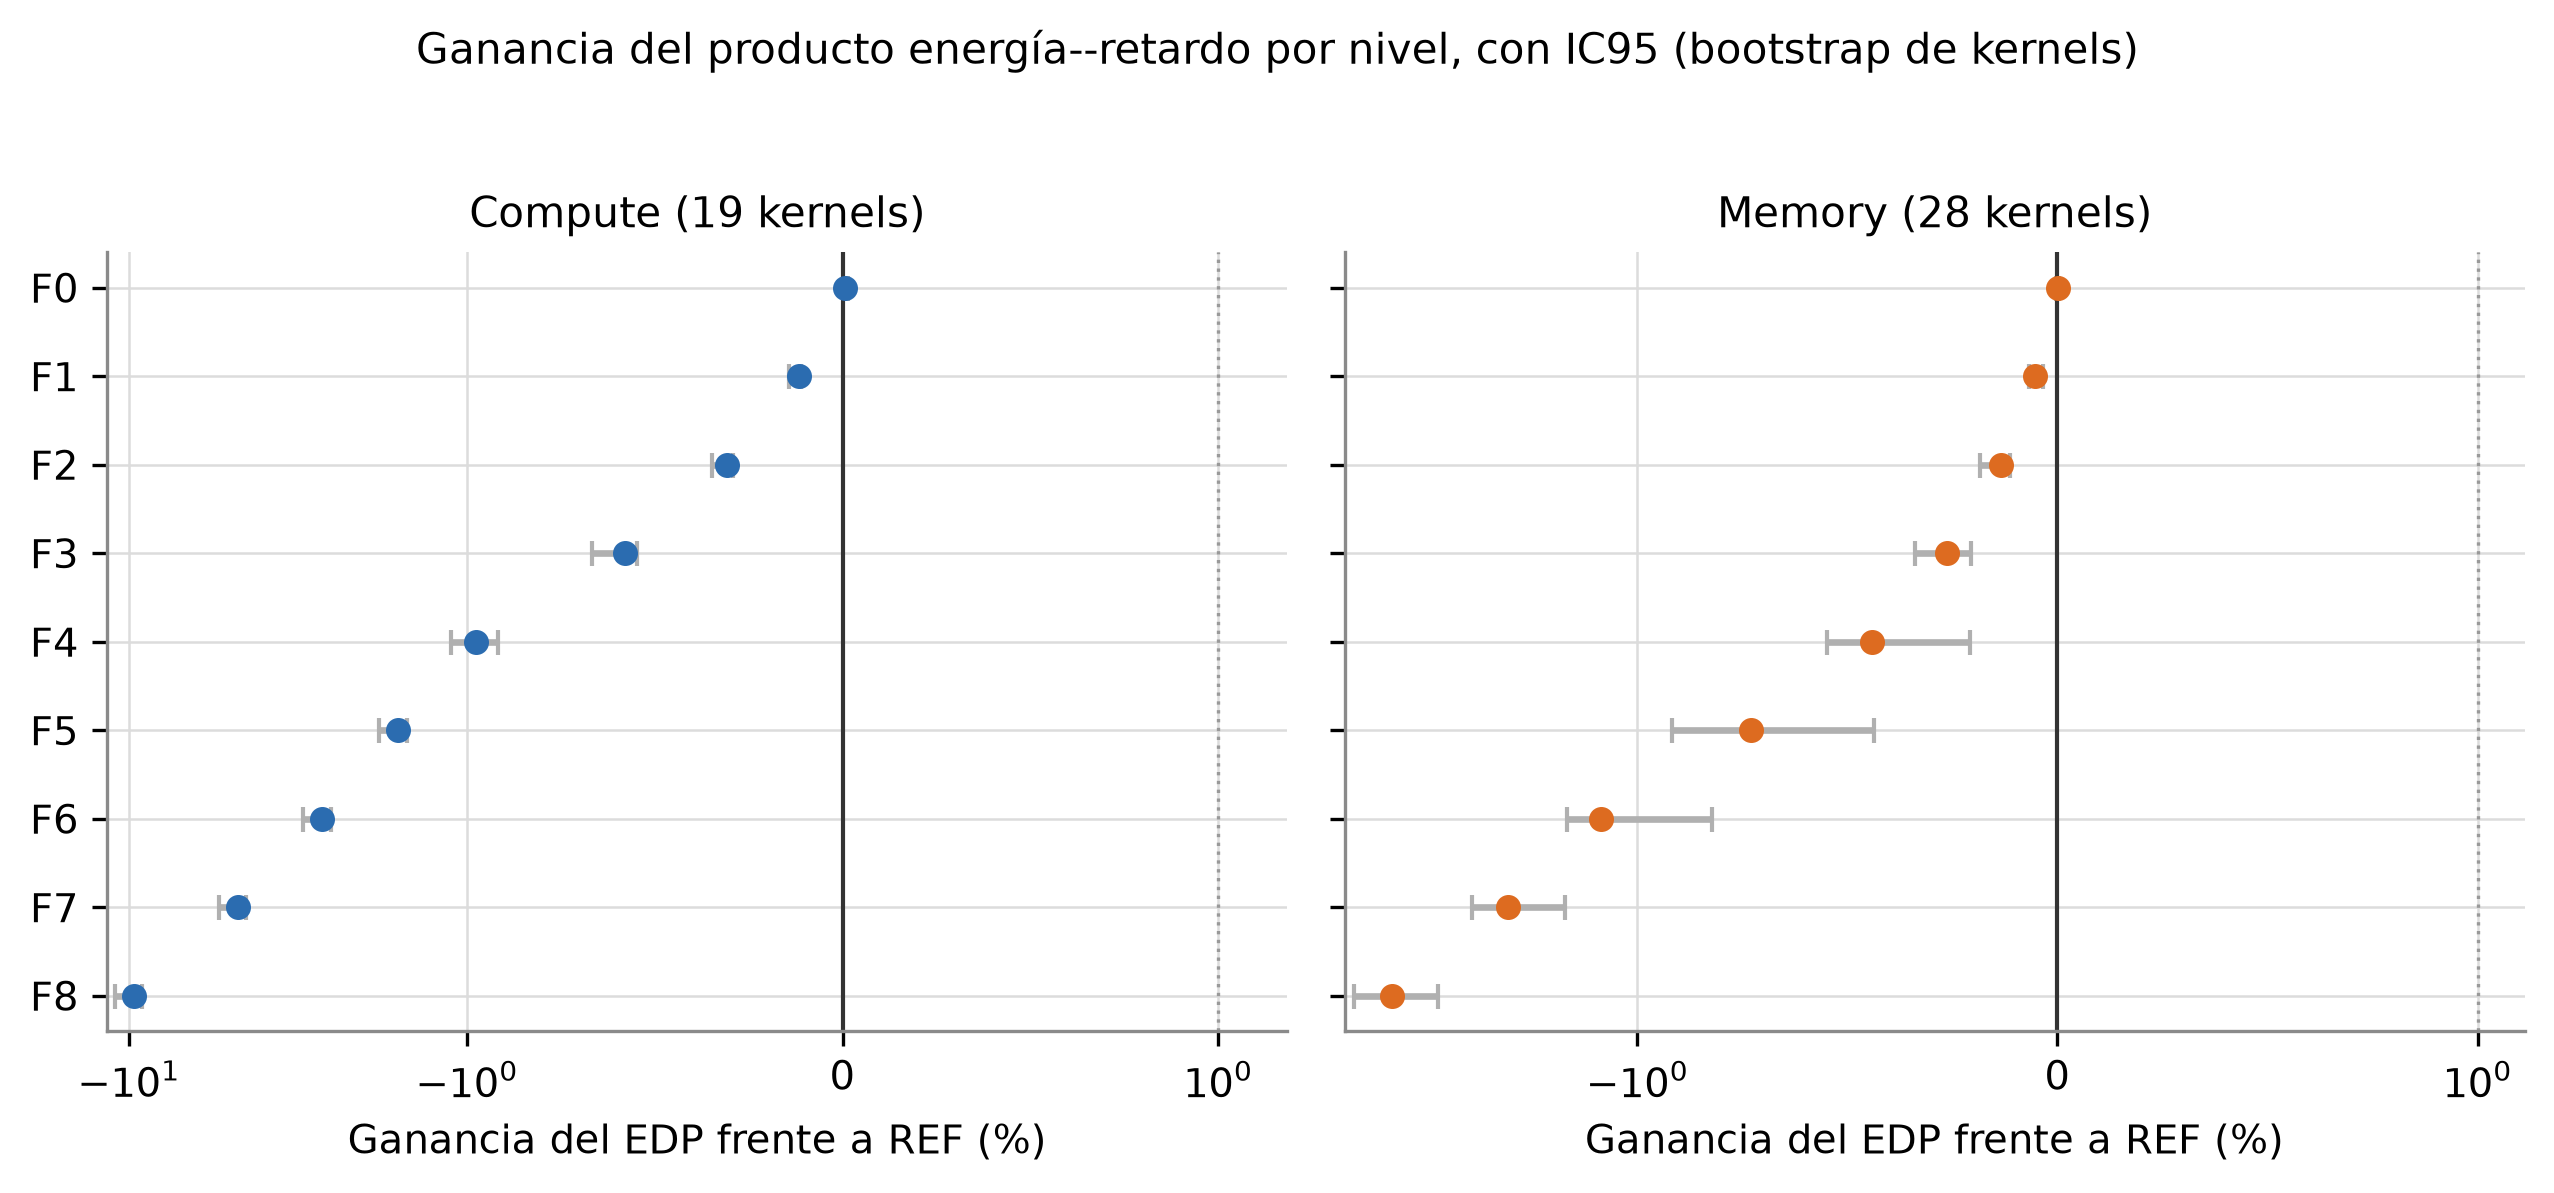
\includegraphics[width=0.85\textwidth]{figuras/fig_cpu_politica_forest_20260922.png}
    \caption[Ganancia del EDP por nivel y clase, en forma de \textit{forest plot}]{La rejilla completa de la Tabla \ref{tab:cpu-politica-detalle}, en forma gráfica. El eje horizontal es simétrico-logarítmico para mostrar a la vez F0, cercano a cero, y F8, con una pérdida de casi un orden de magnitud. Ningún nivel deja el intervalo de confianza por encima de cero de forma útil. Fuente: elaboración propia.}
    \label{fig:cpu-politica-forest}
\end{figure}

\begin{figure}[H]
    \centering
    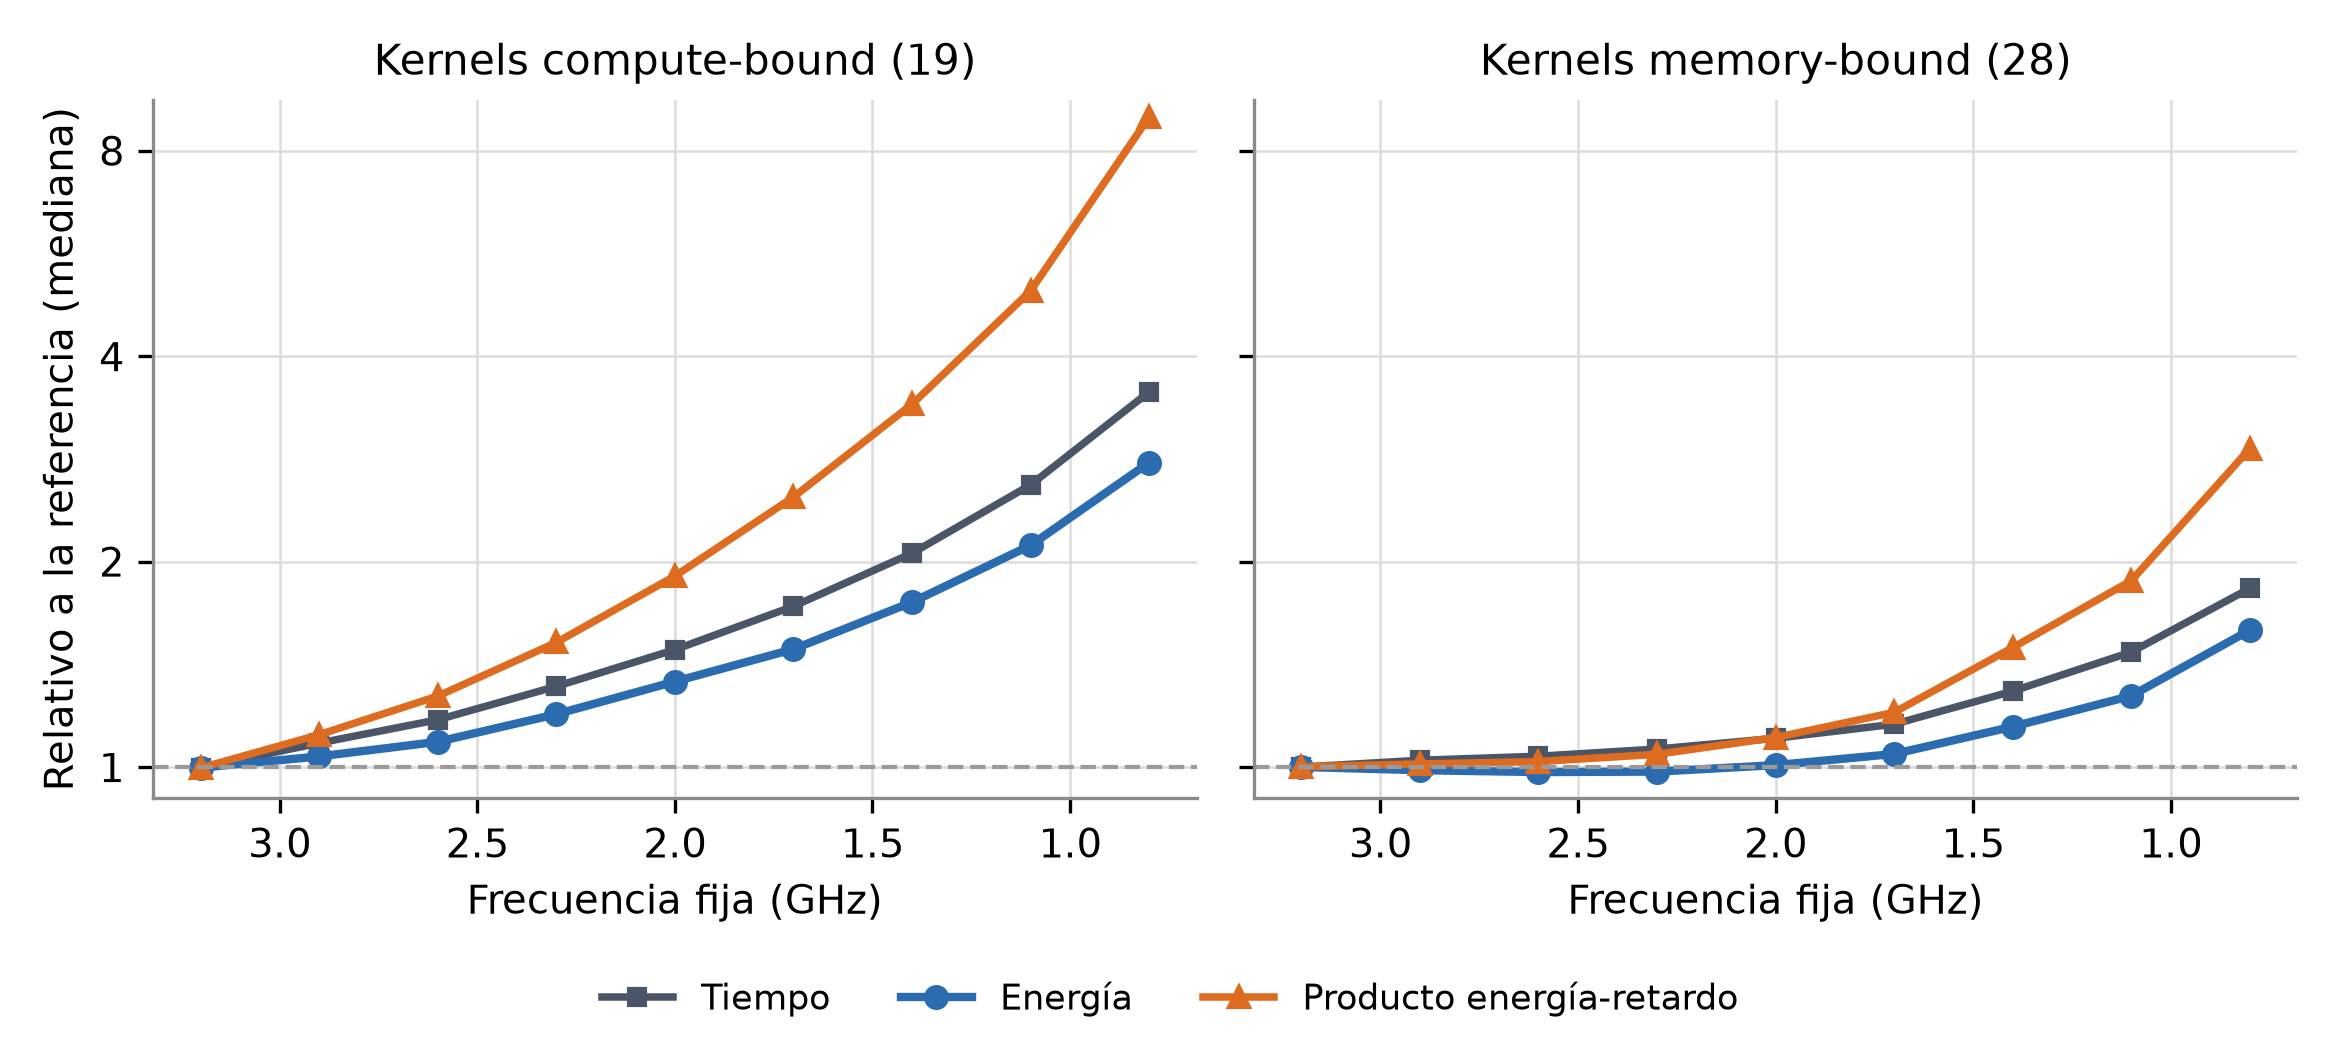
\includegraphics[width=0.94\textwidth]{figuras/fig_cpu_energia_relativa_20260920.png}
    \caption[Energía, tiempo y producto energía--retardo por nivel de frecuencia]{Mediana entre kernels de la energía (paquete y DRAM), el tiempo y el producto energía--retardo de cada nivel fijo, relativos a la referencia nativa, para las dos clases. El eje vertical es logarítmico. Fuente: elaboración propia.}
    \label{fig:cpu-energia-relativa}
\end{figure}

El intervalo de confianza \textit{bootstrap} y el valor $p$ de Wilcoxon de la Tabla \ref{tab:cpu-politica-detalle} responden preguntas distintas y pueden discrepar en apariencia: el primero remuestrea kernels para acotar la ganancia agregada, y el segundo prueba, kernel por kernel, si el signo de la diferencia frente a REF es consistente. Es el caso de F1 y F2 en memory, donde el IC95 excluye el cero pero $p$ no baja de 0.05: con solo 28 kernels y una ganancia heterogénea entre ellos, ambas lecturas son compatibles.

El mecanismo es un piso de potencia de unos 85~W, equivalente al 84\% de la potencia a 3.2~GHz (Figura \ref{fig:cpu-energia-piso}). Reducir la frecuencia a 0.8~GHz ahorra solo 15\% de potencia mientras alarga la ejecución. Incluso un oráculo que eligiera el mejor nivel medido por kernel ganaría 2.2\% en promedio; 22 de 47 kernels quedarían por debajo del efecto mínimo de 1\%. Esta cota es optimista porque el mejor nivel también captura ruido de medición.

\begin{figure}[H]
    \centering
    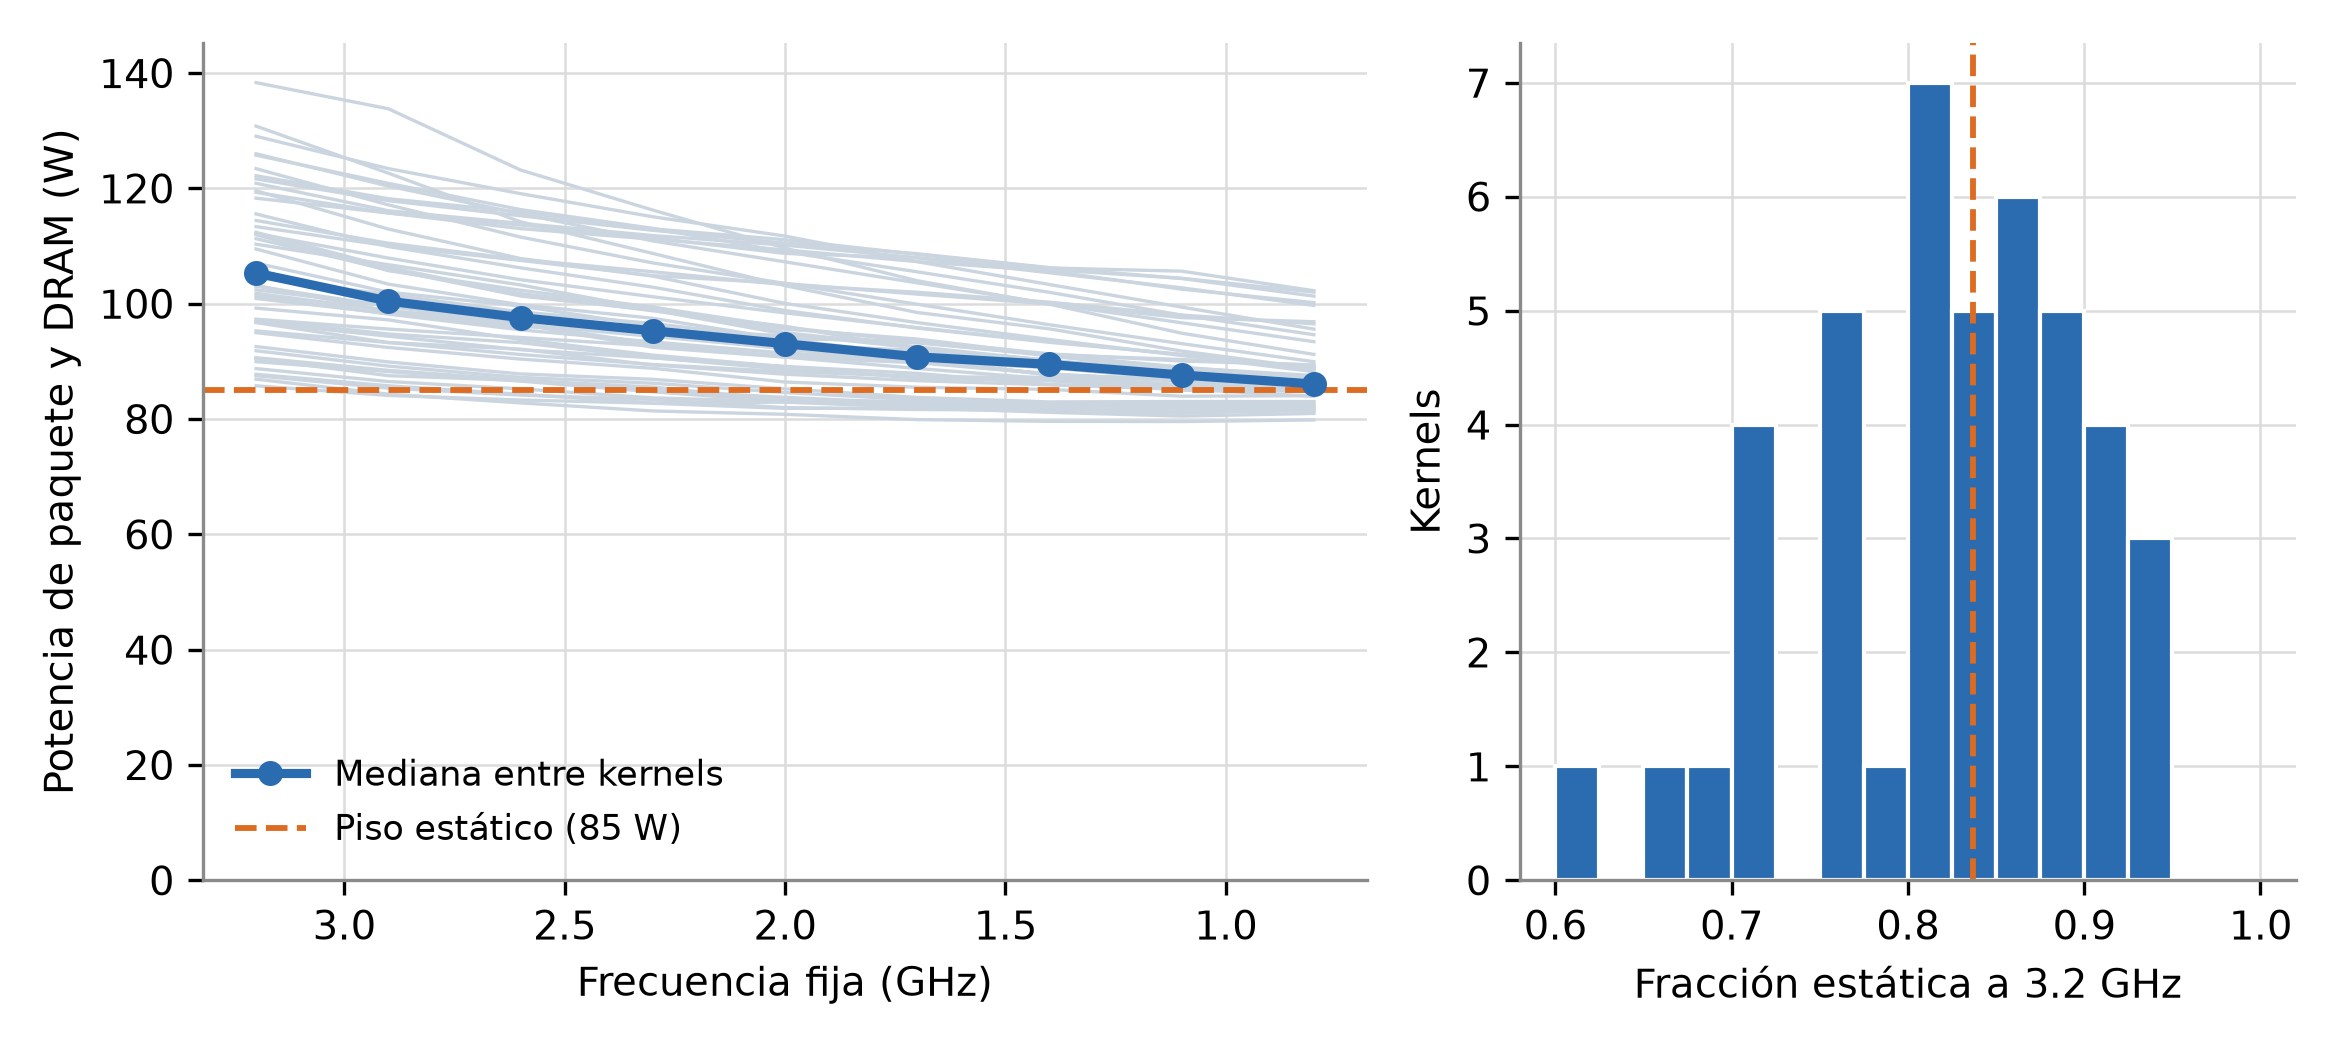
\includegraphics[width=0.94\textwidth]{figuras/fig_cpu_energia_piso_20260920.png}
    \caption[Potencia de paquete y DRAM frente a la frecuencia]{A la izquierda, potencia media de paquete y DRAM de cada kernel (líneas grises) y su mediana en cada nivel fijo, con el piso estático ajustado. A la derecha, distribución entre kernels de la fracción de la potencia a 3.2~GHz que corresponde al piso. Fuente: elaboración propia.}
    \label{fig:cpu-energia-piso}
\end{figure}

\subsubsection{Qué tamaño de efecto podía detectar este diseño}
\label{sec:resultados-cpu-potencia-diseno}

Un resultado de \textit{no actuar} solo es informativo si se acompaña del tamaño de efecto que el experimento podía distinguir, porque de lo contrario no separa la ausencia de efecto de la falta de sensibilidad. Tomando la familia algorítmica como unidad, que es la agrupación con la que se valida el clasificador, la desviación estándar del logaritmo del producto energía--retardo entre repeticiones de una misma combinación tiene mediana de 1.05\%, mientras que la dispersión entre las 19 familias \textit{memory\_bound} es de 5.35\% en F1 y 9.70\% en F2. Es decir, la varianza que limita la conclusión es heterogeneidad física entre cargas, entre cinco y diez veces mayor que el error de medición; aumentar el número de repeticiones no la habría reducido de forma apreciable.

De esas dispersiones se sigue el efecto mínimo detectable con potencia de 80\%: 1.75\% en F0, 3.38\% en F1, 6.05\% en F2 y 9.5\% en F3. La lectura correcta del resultado es, entonces, que con este catálogo quedan descartadas mejoras uniformes superiores a 3.4\% en F1, y que una mejora del orden del 1\%, el efecto mínimo relevante declarado, es indetectable por construcción con 19 familias. Esto acota el resultado en lugar de dejarlo abierto, y es consistente con el piso de potencia descrito arriba: el margen físico disponible es menor que la resolución que el diseño puede ofrecer.

Dado que la clase agregada mezcla cargas con respuestas de signo opuesto, se evaluó además si una regla más fina, condicionada a una variable del vector de entrada, permitía actuar sobre una subpoblación. La regla se congeló antes de medir y se probó en familias nuevas, ajenas a las 30 de entrenamiento, en dos pruebas externas independientes; ambas quedaron refutadas según los criterios declarados de antemano. El detalle queda registrado junto a la tabla de política en \texttt{policy\_cpu.json}. La conclusión operativa de la fase es, por tanto, \textit{no actuar} en ambas clases, sustentada en el piso de potencia medido y no en la ausencia de intentos de refinamiento.

\subsection{Invarianza del clasificador de CPU frente a la acción del agente}
\label{sec:resultados-cpu-frecuencia-contrafactual}

La frecuencia observada es una de las seis variables del clasificador de CPU y el agente la modifica, de modo que se aplicó la misma auditoría contrafactual de la GPU. Sobre el modelo final y sus 1.31 millones de intervalos de 49 kernels, forzar la frecuencia a un valor fijo cambia entre 4 y 11\% de las predicciones (Tabla \ref{tab:cpu-contrafactual-frecuencia}), de modo que existe una dependencia moderada. Pero el cambio que el agente ejecuta es acotado, de F0 (3.2~GHz) a F1 (2.9~GHz): sobre las 179\,774 filas observadas cerca de 3.2~GHz solo cambia el 0.42\% de las predicciones. Con ese espacio de acción la retroalimentación por esta variable es despreciable, y el modelo de CPU se despliega sin modificaciones.



\section{Resultados de GPU}
\label{sec:resultados-gpu}

\subsection{Validación de control y etiquetado}
\label{sec:resultados-gpu-dvfs}
\label{sec:resultados-precision-gpu}

El actuador de GPU sostuvo el bloqueo del reloj de \textit{streaming multiprocessors} bajo carga. Las pruebas con objetivos de 600 y 1200~MHz registraron, respectivamente, 305 y 174 lecturas activas coincidentes con el valor solicitado. La restauración de frecuencia se verificó al finalizar las campañas dedicadas.

La etiqueta Roofline se construyó con la precisión observada mediante Nsight Compute. Este control excluyó kernels con precisión mixta cuya intensidad operacional no admite comparación con un único techo y evitó atribuir a los contadores convencionales el trabajo ejecutado por Tensor Cores. En el nivel de referencia, los puntos de inflexión medidos fueron 14.965852~FLOP/byte para FP32 y 6.898377~FLOP/byte para FP64.

\subsection{Diagnóstico del primer conjunto GPU}
\label{sec:resultados-gpu-dataset-final}
\label{sec:resultados-gpu-separabilidad}

La primera campaña GPU reunió 540 corridas planificadas para 18 kernels. Después de calibrar el warmup, 334 corridas de 16 kernels y 11 familias quedaron disponibles para el diagnóstico inicial. El conjunto estaba desbalanceado (Figura \ref{fig:gpu-balance-clases-final}), con 73 corridas \textit{compute\_bound} y 261 \textit{memory\_bound}, y la mayoría de las familias era homogénea respecto de su etiqueta.

El árbol de profundidad 1 obtuvo un F1 macro de 0.617 bajo validación \textit{leave-one-familia-out}, frente a 0.553 del clasificador mayoritario. Este valor no se adopta como resultado final. La evaluación mostró que, al retirar familias completas, muchos pliegues quedaban sin ejemplos de una clase. Además, la utilización de SM no separó de forma universal los dos regímenes. \textit{rodinia\_gaussian}, por ejemplo, fue \textit{memory\_bound} según Roofline, pero alcanzó utilizaciones de SM suficientemente altas para que el modelo lo confundiera con una carga \textit{compute\_bound}.

La evidencia no indicó que bastara ajustar el modelo sobre el mismo conjunto. Mostró que faltaban familias \textit{compute\_bound} variadas y alejadas del punto de inflexión. Por esta razón se cambió la estrategia desde la búsqueda de hiperparámetros hacia la ampliación experimental del catálogo y la revisión del protocolo de validación.

\begin{figure}[H]
    \centering
    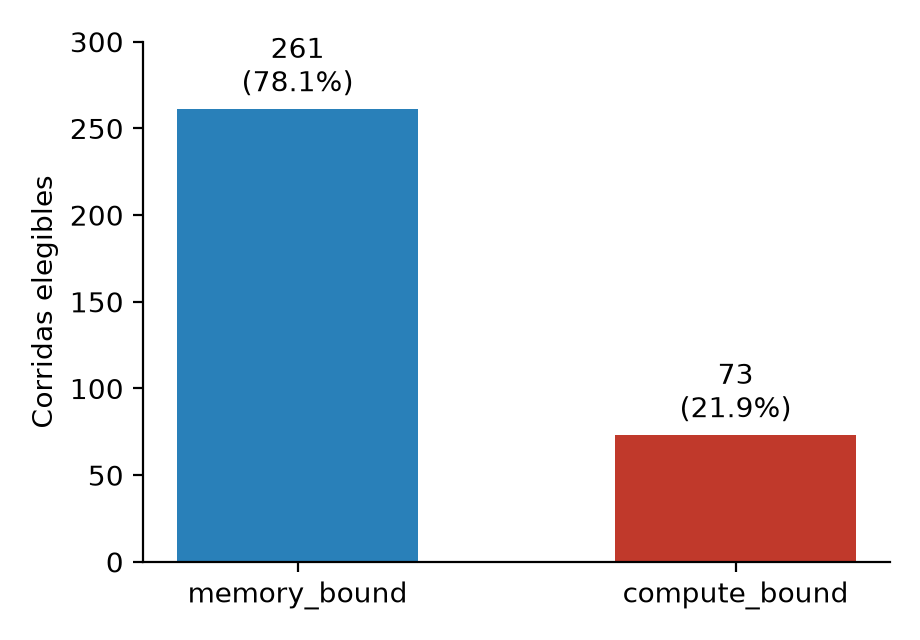
\includegraphics[width=0.5\textwidth]
        {figuras/fig_gpu_balance_clases_final_20260915.png}
    \caption[Balance de clases del conjunto GPU inicial]{Distribución de las 334 corridas elegibles del conjunto GPU empleado en el diagnóstico exploratorio. Fuente: elaboración propia.}
    \label{fig:gpu-balance-clases-final}
\end{figure}

\subsection{Reanálisis de campañas históricas con NVML}
\label{sec:resultados-gpu-oi-ventana}
\label{sec:resultados-gpu-gemm-evolucion}

El bloqueo de la nueva campaña multi-frecuencia impidió incorporar observaciones nuevas durante buena parte de esta fase. Se reanalizaron entonces campañas ya aceptadas, cuya etiqueta Roofline fue construida fuera de línea con \texttt{ncu} y cuya inferencia potencial dependía exclusivamente de NVML. El posproceso comparó esa intensidad con el \textit{ridge} correspondiente a la frecuencia y precisión de cada corrida, y difundió la misma etiqueta a todas sus lecturas NVML. No se registraron eventos CUPTI de lanzamiento en estas campañas, así que cada corrida se transformó en una sola observación mediante agregados robustos, sin duplicar ni sintetizar observaciones.

Un primer diagnóstico sobre esta representación mostró separación parcial entre clases (Figura \ref{fig:gpu-separabilidad-nvml}): la proyección PCA conserva la estructura global y t-SNE aproxima los vecindarios locales de ocho variables estáticas (mediana e IQR de utilización GPU, utilización de memoria, potencia y reloj SM). Ambas vistas contienen regiones dominadas por una clase, pero también regiones con etiquetas mezcladas. La separación por clase, calculada en el espacio original estandarizado, tuvo un coeficiente de silueta de 0.092, que describe separación débil. Un clasificador de tres vecinos que nunca observa ejemplos de la familia evaluada alcanzó F1 macro de 0.616, coherente con una señal transferible parcial: existe información física real en los agregados NVML, pero no una frontera estable para todas las familias.

\begin{figure}[H]
    \centering
    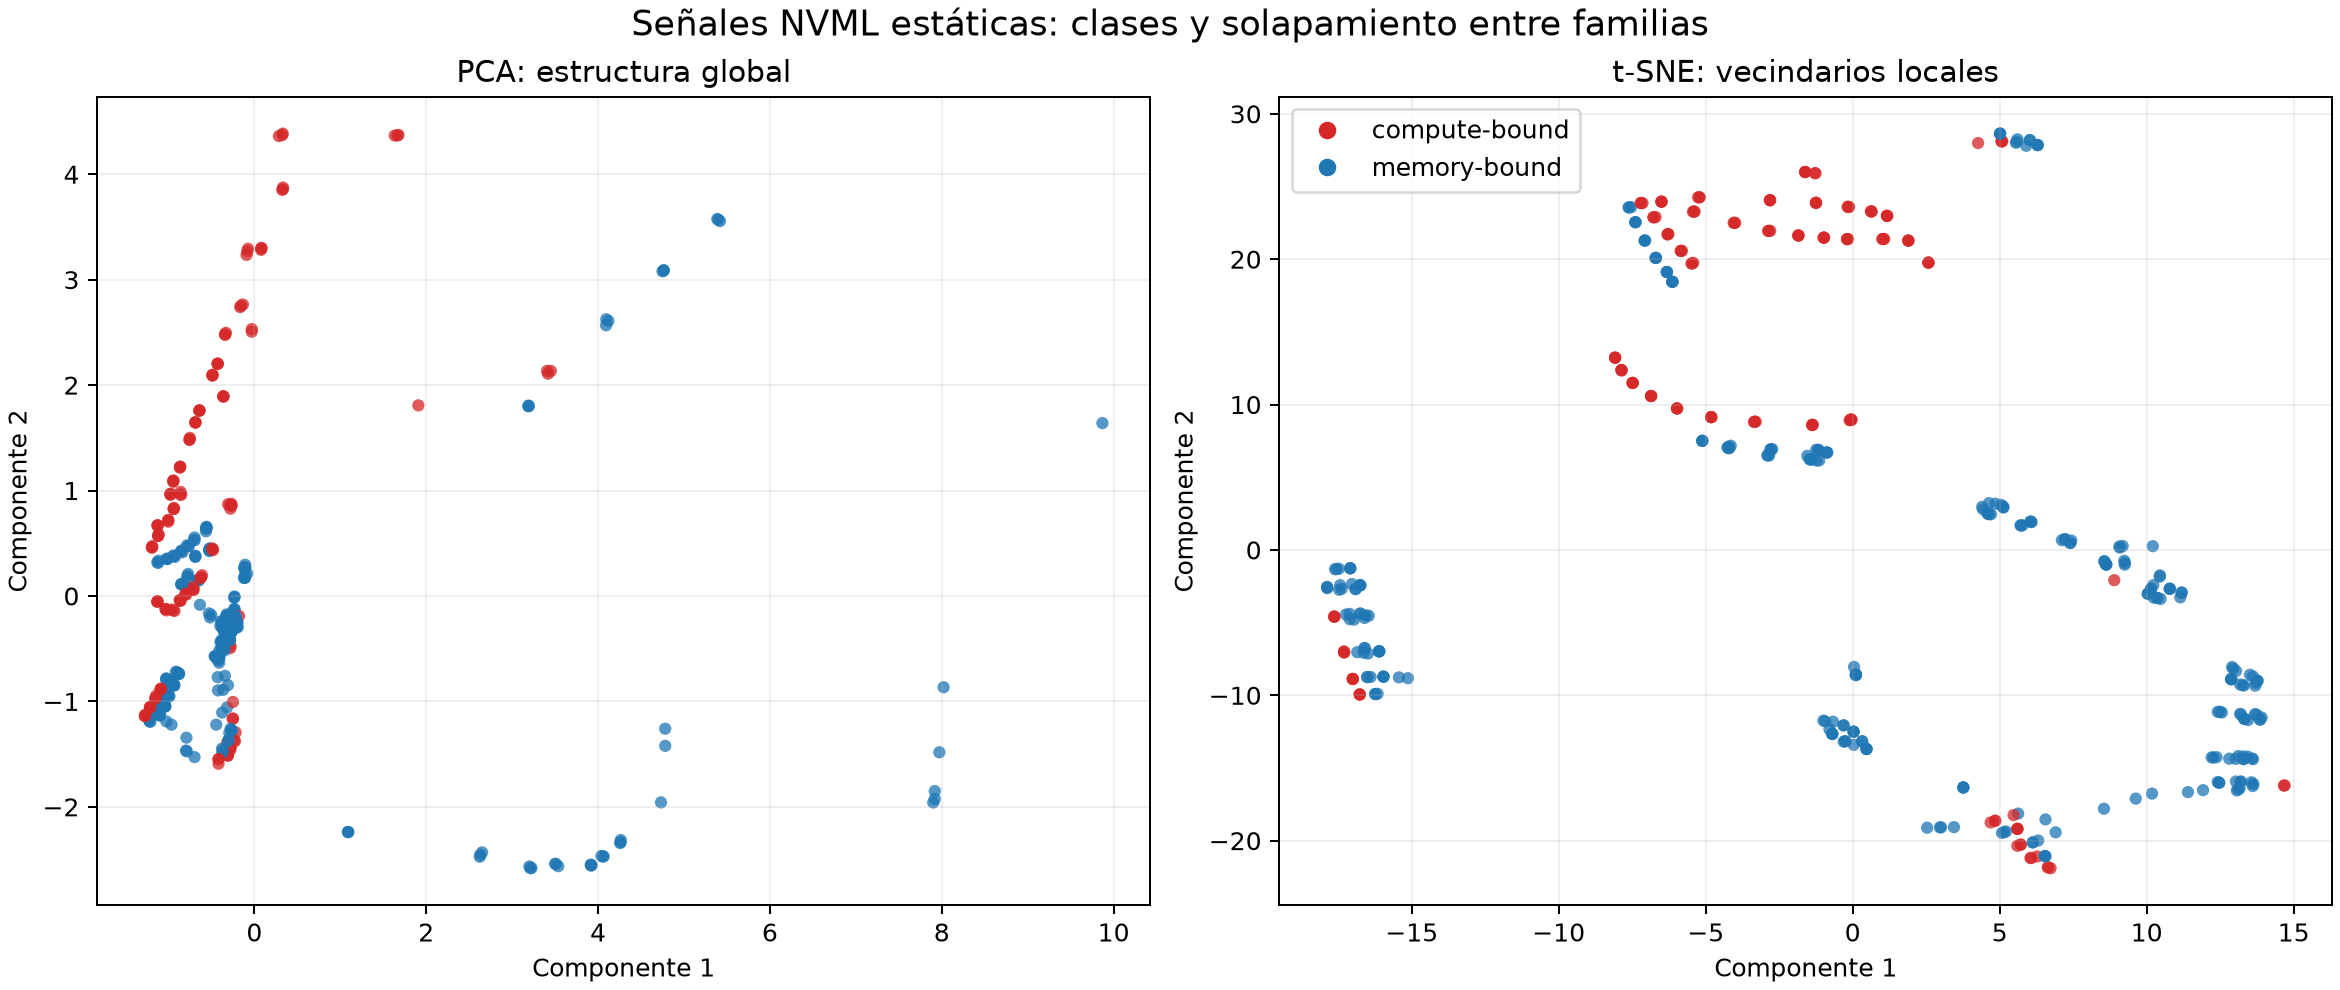
\includegraphics[width=\textwidth]
        {figuras/fig_gpu_separabilidad_nvml_20260918.png}
    \caption[Separabilidad de las clases GPU con señales NVML]{Proyecciones PCA y t-SNE de las medianas e IQR de utilización GPU, utilización de memoria, potencia y reloj SM. La proyección t-SNE es diagnóstica y no se utiliza para medir generalización. Fuente: elaboración propia.}
    \label{fig:gpu-separabilidad-nvml}
\end{figure}

A partir de ese diagnóstico se amplió el conjunto fusionando las campañas modernas aceptadas con tres campañas adicionales ya cerradas (\textit{kmeans}, miniBUDE y \textit{conv2d}), y se admitieron corridas que el gate de calidad había descartado únicamente por tener una fracción de muestras NVML posteriores al arranque menor al 50\%, cuando el conteo absoluto de muestras seguía siendo alto (cientos a miles por corrida). El conjunto resultante tiene 483 corridas y 16 familias algorítmicas, separando además los tres núcleos CUDA de RAJAPerf (GEMM, \textit{stencil} de calor y Jacobi 2D) que antes compartían una sola familia pese a tener perfiles Roofline distintos entre sí. La composición es de 171 corridas \textit{compute\_bound} y 312 \textit{memory\_bound}, trece de las dieciséis familias homogéneas respecto de su etiqueta.

La métrica de evaluación pasó a ser la exactitud balanceada sobre celdas familia por clase, el promedio del \textit{recall} de cada combinación observada. Esta métrica está bien definida incluso en familias de una sola clase y no depende de la prevalencia relativa de cada familia, a diferencia del F1 macro agrupado por volumen. La validación usó \textit{leave-one-familia-out}, cinco semillas de muestreo y un intervalo de confianza del 95\% por remuestreo \textit{bootstrap} de familias (2000 réplicas). Se compararon siete modelos candidatos con hiperparámetros fijos (Tabla \ref{tab:gpu-modelos-2026-09-22} y Figura \ref{fig:gpu-comparacion-modelos}): ninguno domina de forma concluyente. \textit{Random forest} (0.807), \textit{extra trees} (0.806) y la regresión logística (0.792) resultaron estadísticamente indistinguibles entre sí por remuestreo pareado de familias (probabilidad de superioridad entre 0.53 y 0.60), aunque \textit{random forest} sí superó con evidencia razonable a XGBoost (probabilidad de superioridad 0.961).

\begin{figure}[H]
    \centering
    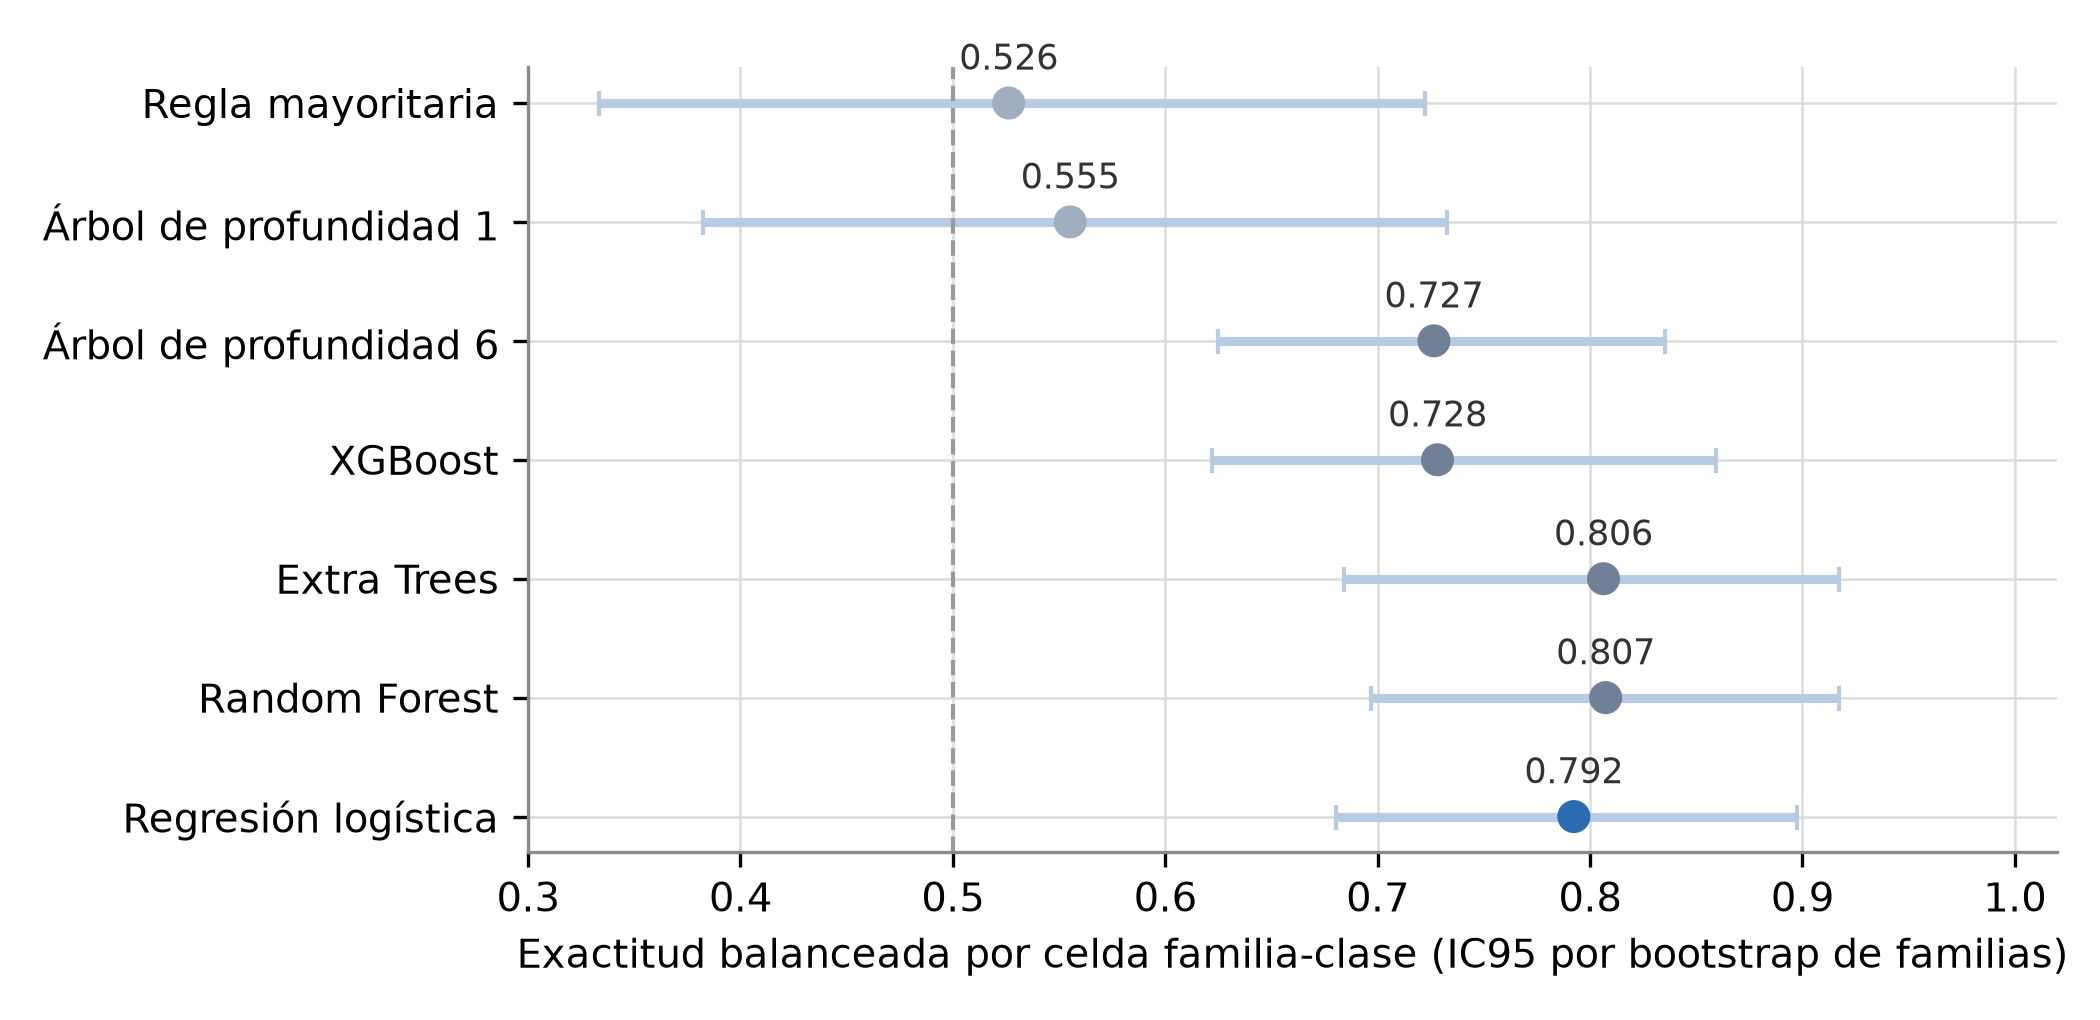
\includegraphics[width=\textwidth]{figuras/fig_gpu_comparacion_modelos_20260922.png}
    \caption[Comparación de modelos candidatos GPU]{Exactitud balanceada por celda familia-clase de los siete modelos candidatos, con intervalo de confianza del 95\% por \textit{bootstrap} de familias. Fuente: elaboración propia.}
    \label{fig:gpu-comparacion-modelos}
\end{figure}



Las cinco variables del conjunto candidato (Tabla \ref{tab:gpu-vif}) no presentan colinealidad relevante: el factor de inflación de varianza (VIF) máximo fue 2.26, muy por debajo del umbral convencional de 5 que suele usarse como señal de alerta.



Una búsqueda anidada de hiperparámetros con muestreador TPE (\textit{Optuna}), quince pruebas por modelo dentro de un \textit{leave-one-familia-out} interno, empeoró el resultado en cuatro de los cinco modelos ajustables respecto de la configuración fija (regresión logística de 0.792 a 0.767, \textit{random forest} de 0.807 a 0.778, \textit{extra trees} de 0.806 a 0.748, XGBoost de 0.740 a 0.724; solo el árbol de profundidad 6 mejoró, de 0.727 a 0.783). El mismo mecanismo documentado para el clasificador de fase de CPU explica esta caída: con familias limitadas, el criterio interno que Optuna maximiza no discrimina de forma confiable la configuración que generaliza mejor. La búsqueda de hiperparámetros se descarta para el candidato GPU por la misma razón que para CPU.

Con el empate entre \textit{random forest}, \textit{extra trees} y regresión logística ya establecido, el criterio de desempate para la referencia estática fue la latencia de inferencia de una sola fila, medida en \texttt{paccaA100}, el nodo de destino real. La regresión logística respondió en 400.9, 413.8 y 466.9 microsegundos (percentiles 50, 95 y 99); \textit{random forest} y \textit{extra trees} tardaron entre diez y doce veces más (percentil 99 de 5512.2 y 4989.9 microsegundos, respectivamente). La regresión logística usa las cuatro señales NVML, utilización GPU, utilización de memoria, potencia y reloj SM, todas por mediana, más la desviación estándar intracorrida de la utilización de memoria como quinta variable. Esta última se incorporó porque las medianas por sí solas diluyen el efecto de cargas con lanzamientos cortos y repetidos, como \textit{kmeans}, cuya intensidad operacional real es alta pero cuya firma NVML agregada se asemeja a una carga poco ocupada.

Dos familias no se resuelven con ninguna de las variables disponibles por una razón física, no por una limitación del modelo: el núcleo GEMM de RAJAPerf y \textit{LUD} de Rodinia cambian de régimen Roofline según el nivel de frecuencia de la corrida, porque el punto de inflexión se desplaza con el reloj mientras la intensidad operacional de cada kernel permanece fija. \textit{LUD}, por ejemplo, resultó \textit{memory\_bound} en los niveles de reloj más altos y \textit{compute\_bound} en los más bajos de la misma familia. Distinguir ese cambio exigiría una variable de distancia al \textit{ridge}, que constituye fuga de la propia etiqueta y por tanto no es admisible como entrada del clasificador.

La Figura \ref{fig:gpu-resultado-por-familia} desagrega el desempeño de la regresión logística estática por familia. El resultado no es parejo: ocho de las dieciséis familias superan 0.90 de exactitud, mientras \textit{dual\_cholesky} (0.23), el núcleo GEMM de RAJAPerf (0.50, la familia con cruce de \textit{ridge} ya descrita) y \textit{rodinia\_gaussian} (0.53, la familia más cercana al \textit{ridge} del catálogo) quedan por debajo del umbral trivial de 0.5. La matriz de confusión agregada (Figura \ref{fig:gpu-matriz-confusion}, panel izquierdo) resume esto en 483 corridas: 125 de 171 \textit{compute\_bound} (73.1\%) y 247 de 312 \textit{memory\_bound} (79.2\%) correctamente clasificadas.

\begin{figure}[H]
    \centering
    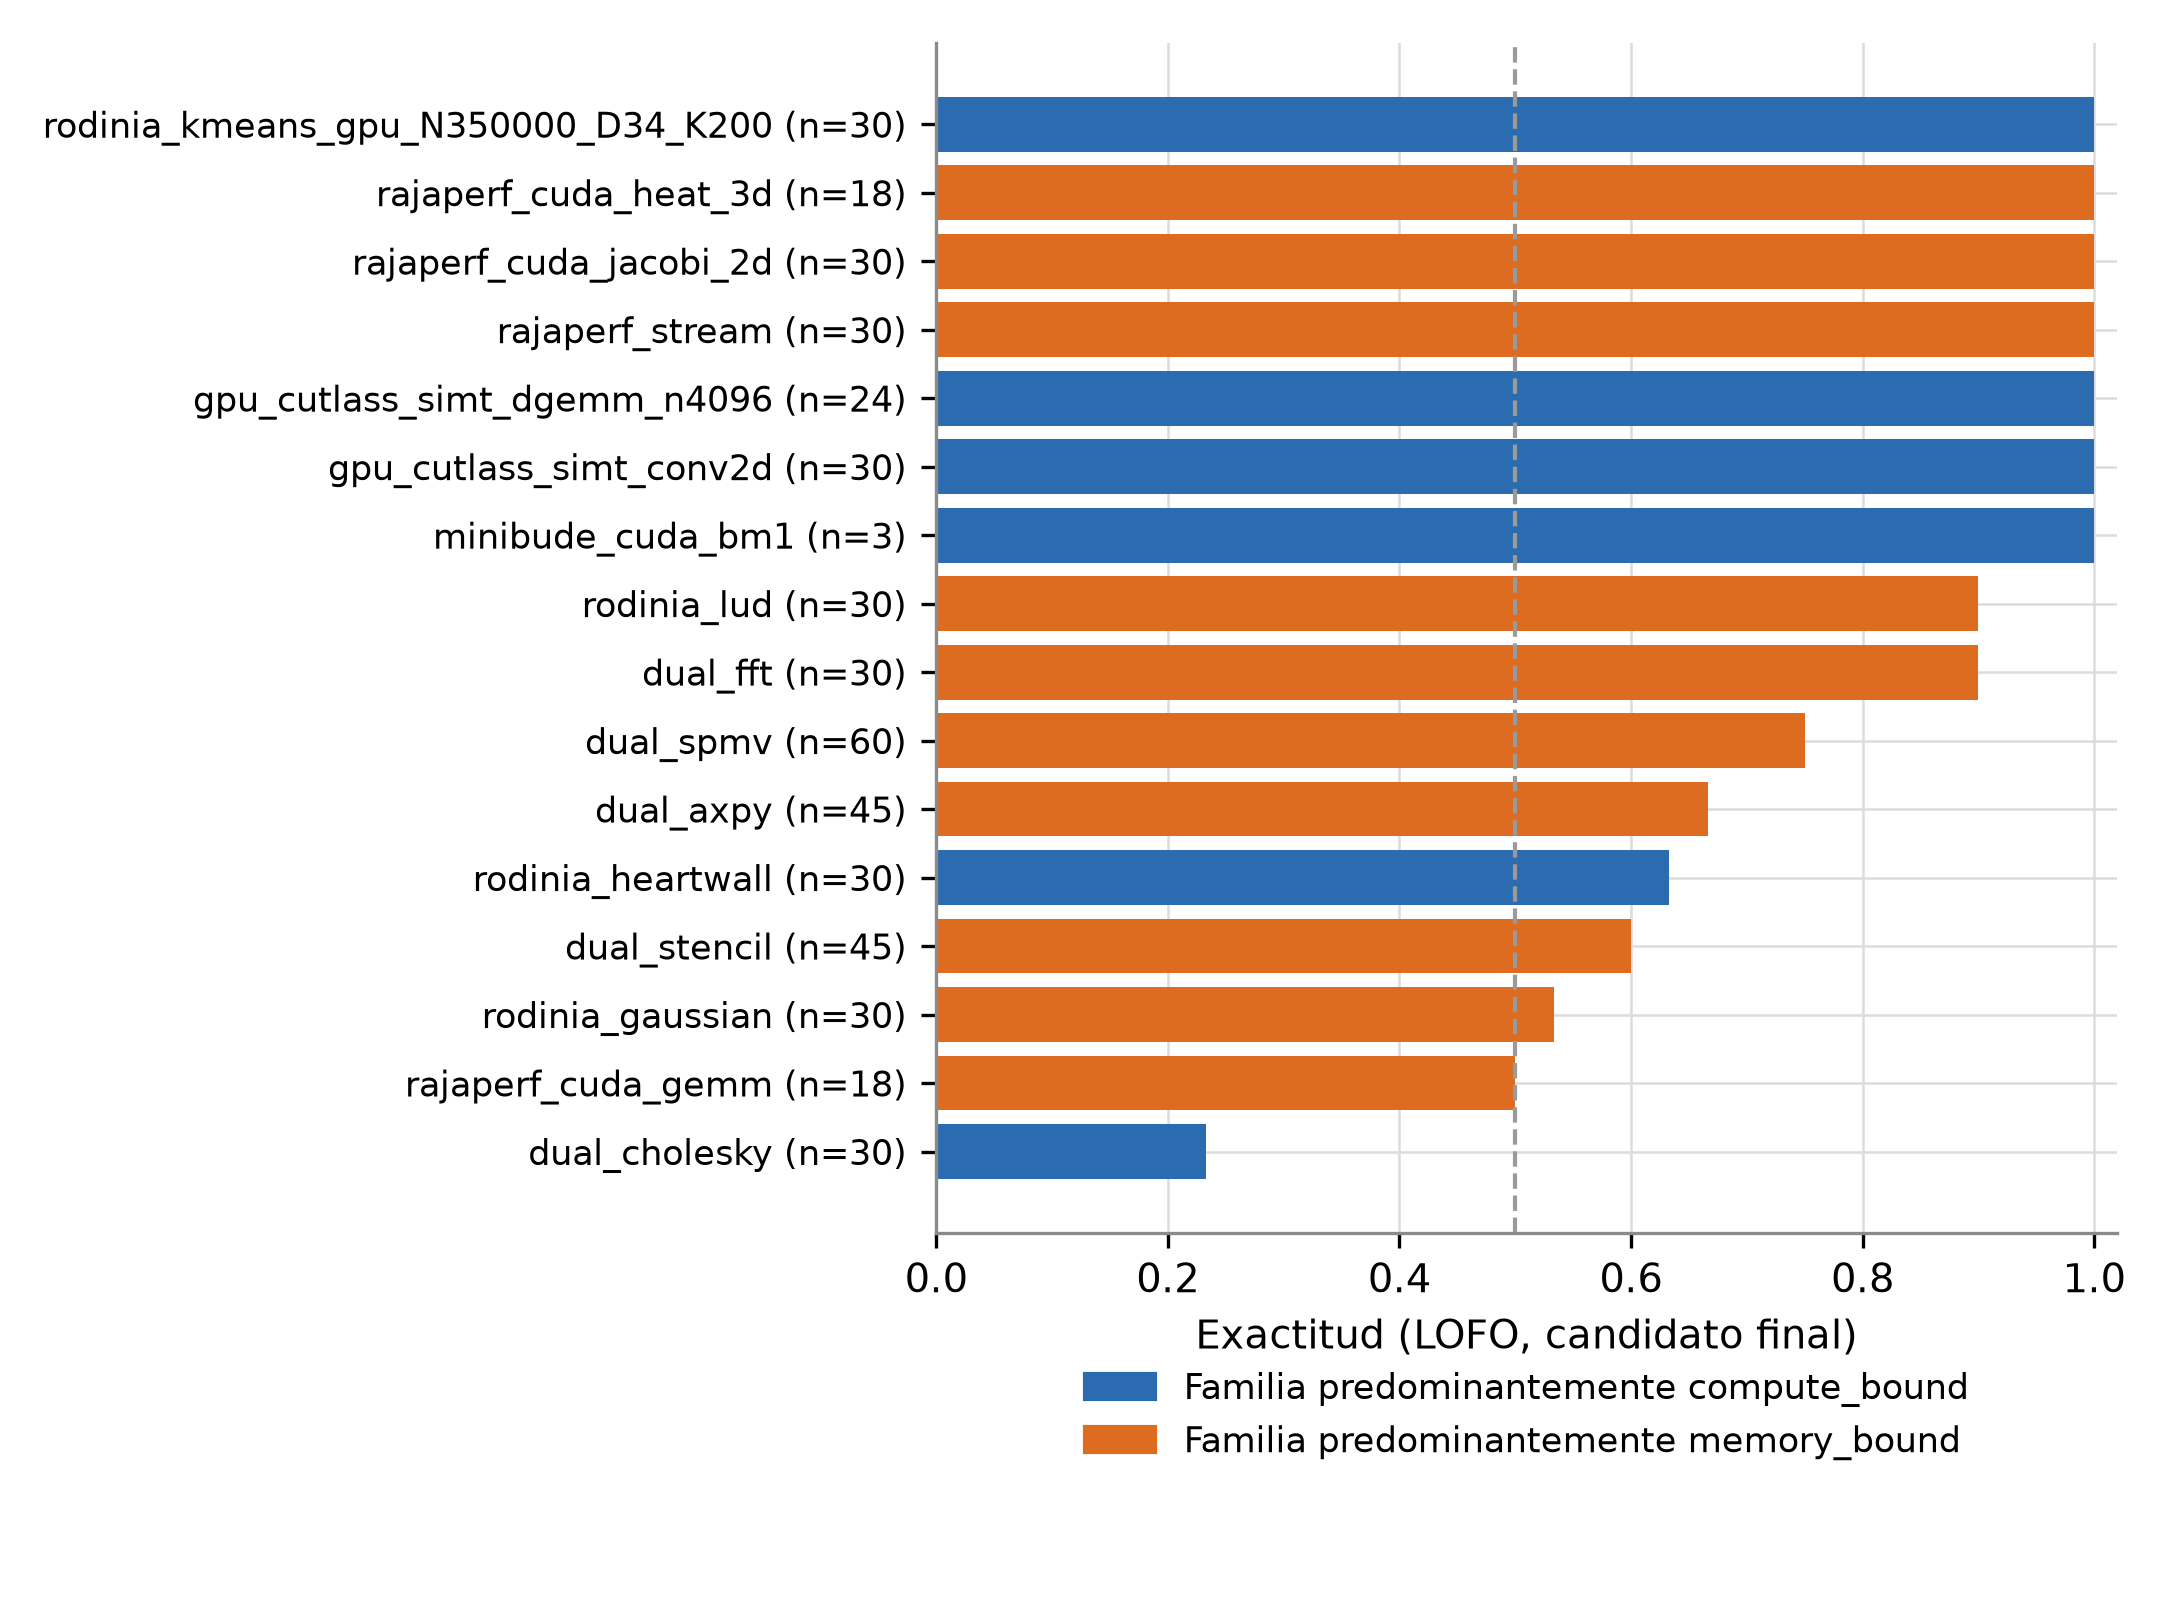
\includegraphics[width=\textwidth]{figuras/fig_gpu_resultado_por_familia_20260922.png}
    \caption[Exactitud de la referencia estática GPU por familia]{Exactitud de la regresión logística de cinco entradas por familia algorítmica, LOFO. El color indica la clase predominante real de cada familia. Fuente: elaboración propia.}
    \label{fig:gpu-resultado-por-familia}
\end{figure}





La calibración de probabilidades de la regresión logística de cinco variables, usada aquí solo como candidato estático de referencia, tiene un error de calibración esperado (ECE, calculado sobre diez rangos de confianza de igual amplitud) de 0.057. Su umbral de 0.70 sube la exactitud balanceada por celda de 0.792 a 0.846 reteniendo el 76.7\% de las corridas (Figura \ref{fig:gpu-calibracion-umbral}). La selección del modelo desplegable se reporta por separado después de aplicar el contrato de entradas invariantes.

\begin{figure}[H]
    \centering
    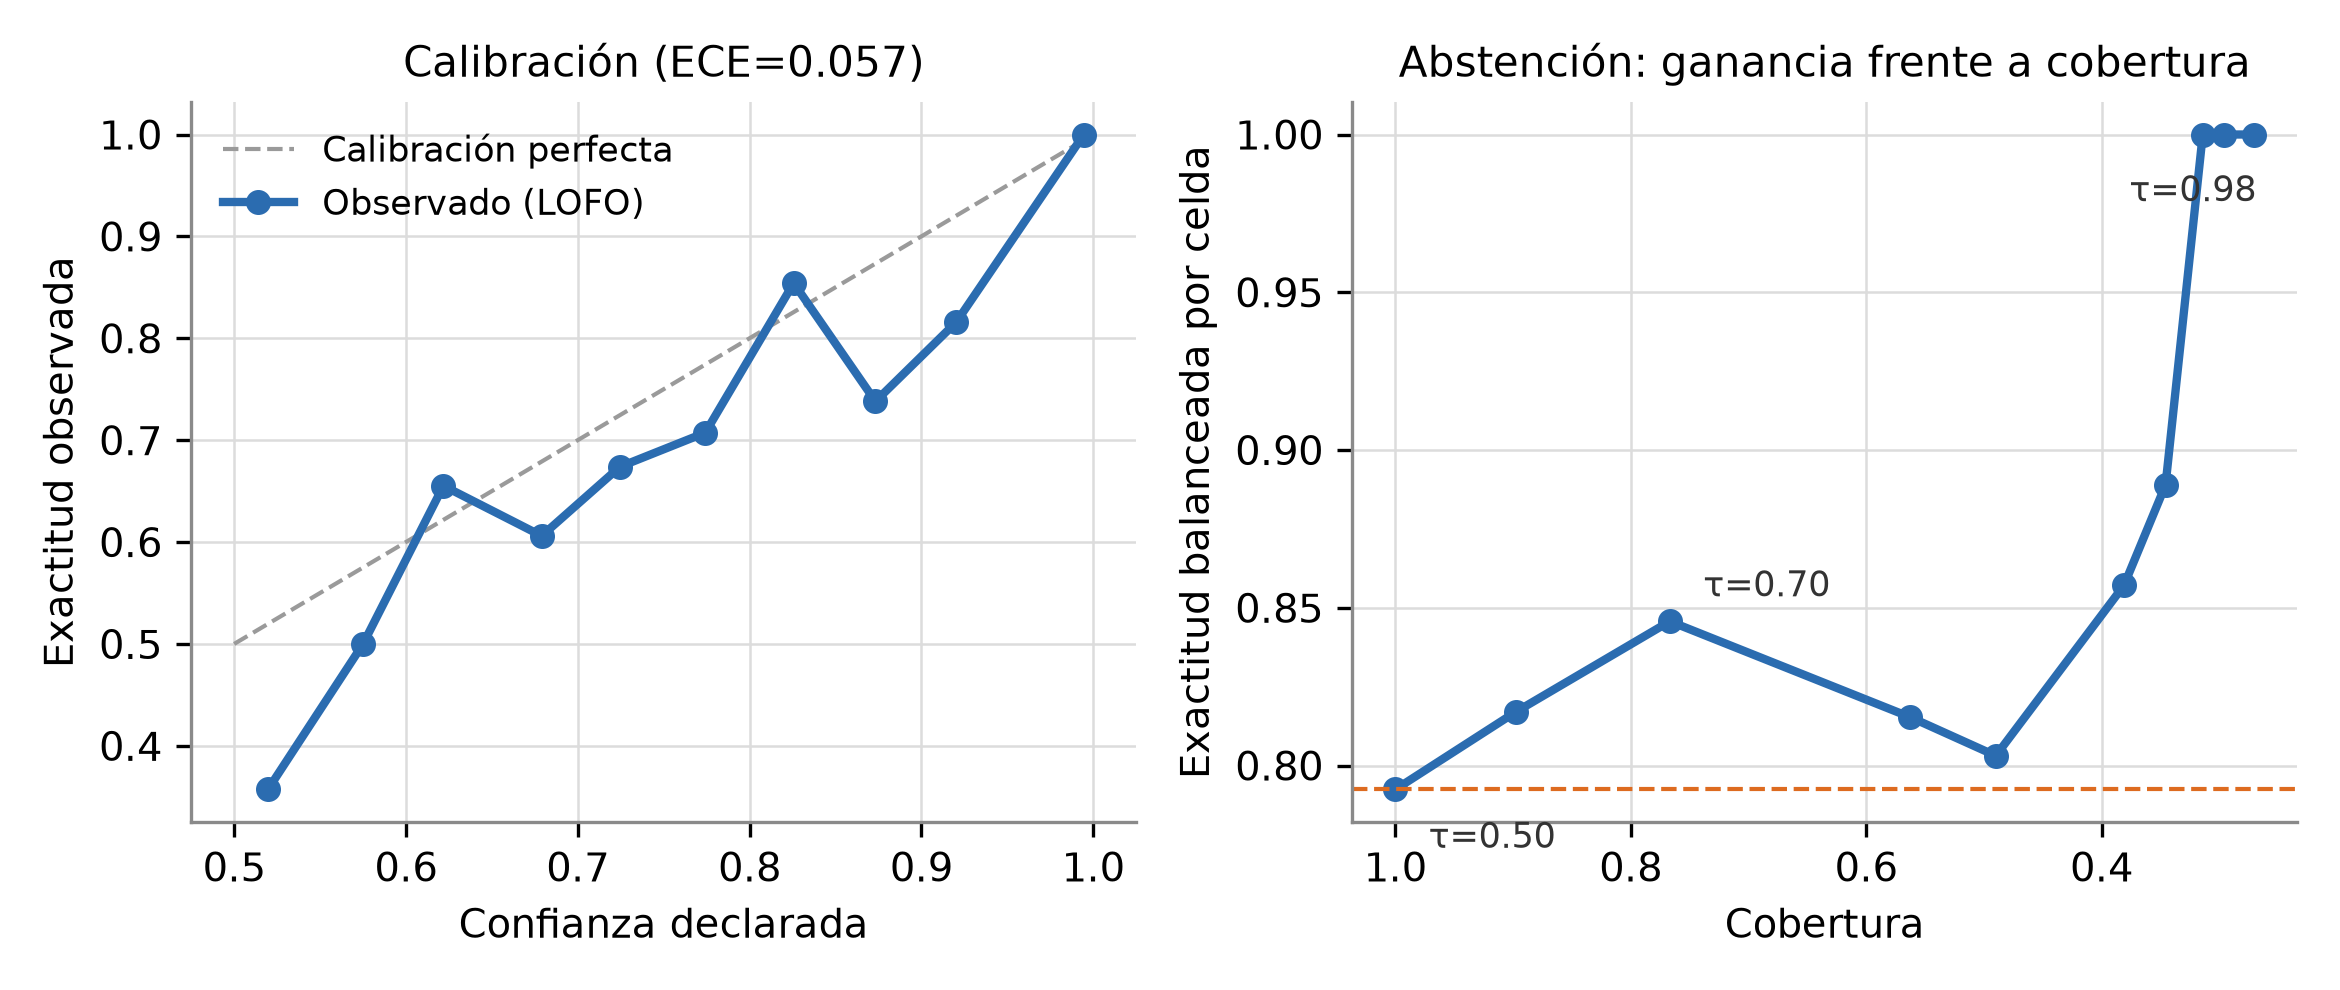
\includegraphics[width=\textwidth]{figuras/fig_gpu_calibracion_umbral_20260922.png}
    \caption[Calibración y abstención de la regresión logística GPU]{Calibración y abstención de la regresión logística de cinco entradas, candidata estática que no se despliega en el agente. Izquierda, confianza declarada contra exactitud observada, agrupada en diez rangos de igual amplitud. Derecha, exactitud balanceada por celda contra cobertura para distintos umbrales de decisión $\tau$. Fuente: elaboración propia.}
    \label{fig:gpu-calibracion-umbral}
\end{figure}

La regresión logística estática ya congelada, con sus cinco entradas, se evaluó una vez contra cuatro familias de Rodinia de una campaña de agosto (Backprop, DWT2D, LavaMD y Myocyte) que no participaron en ninguna decisión de esta ronda: ni en el umbral de aceptación de corridas, ni en la separación de familias de RAJAPerf, ni en la variable de variabilidad añadida, ni en la elección del modelo. Es el equivalente honesto a un conjunto de prueba sellado para esa referencia. Sobre 140 corridas, la exactitud global fue 0.779 (Figura \ref{fig:gpu-matriz-confusion}, panel derecho), con \textit{LavaMD} como la familia más débil (0.5) y las otras tres entre 0.81 y 0.97. Esta cifra es consistente con una validación externa independiente reportada en una versión anterior de este análisis sobre un conjunto ligeramente distinto (exactitud 0.743, misma familia más débil), lo que respalda que el resultado no es un artefacto de la partición específica de esta ronda.

\begin{figure}[H]
    \centering
    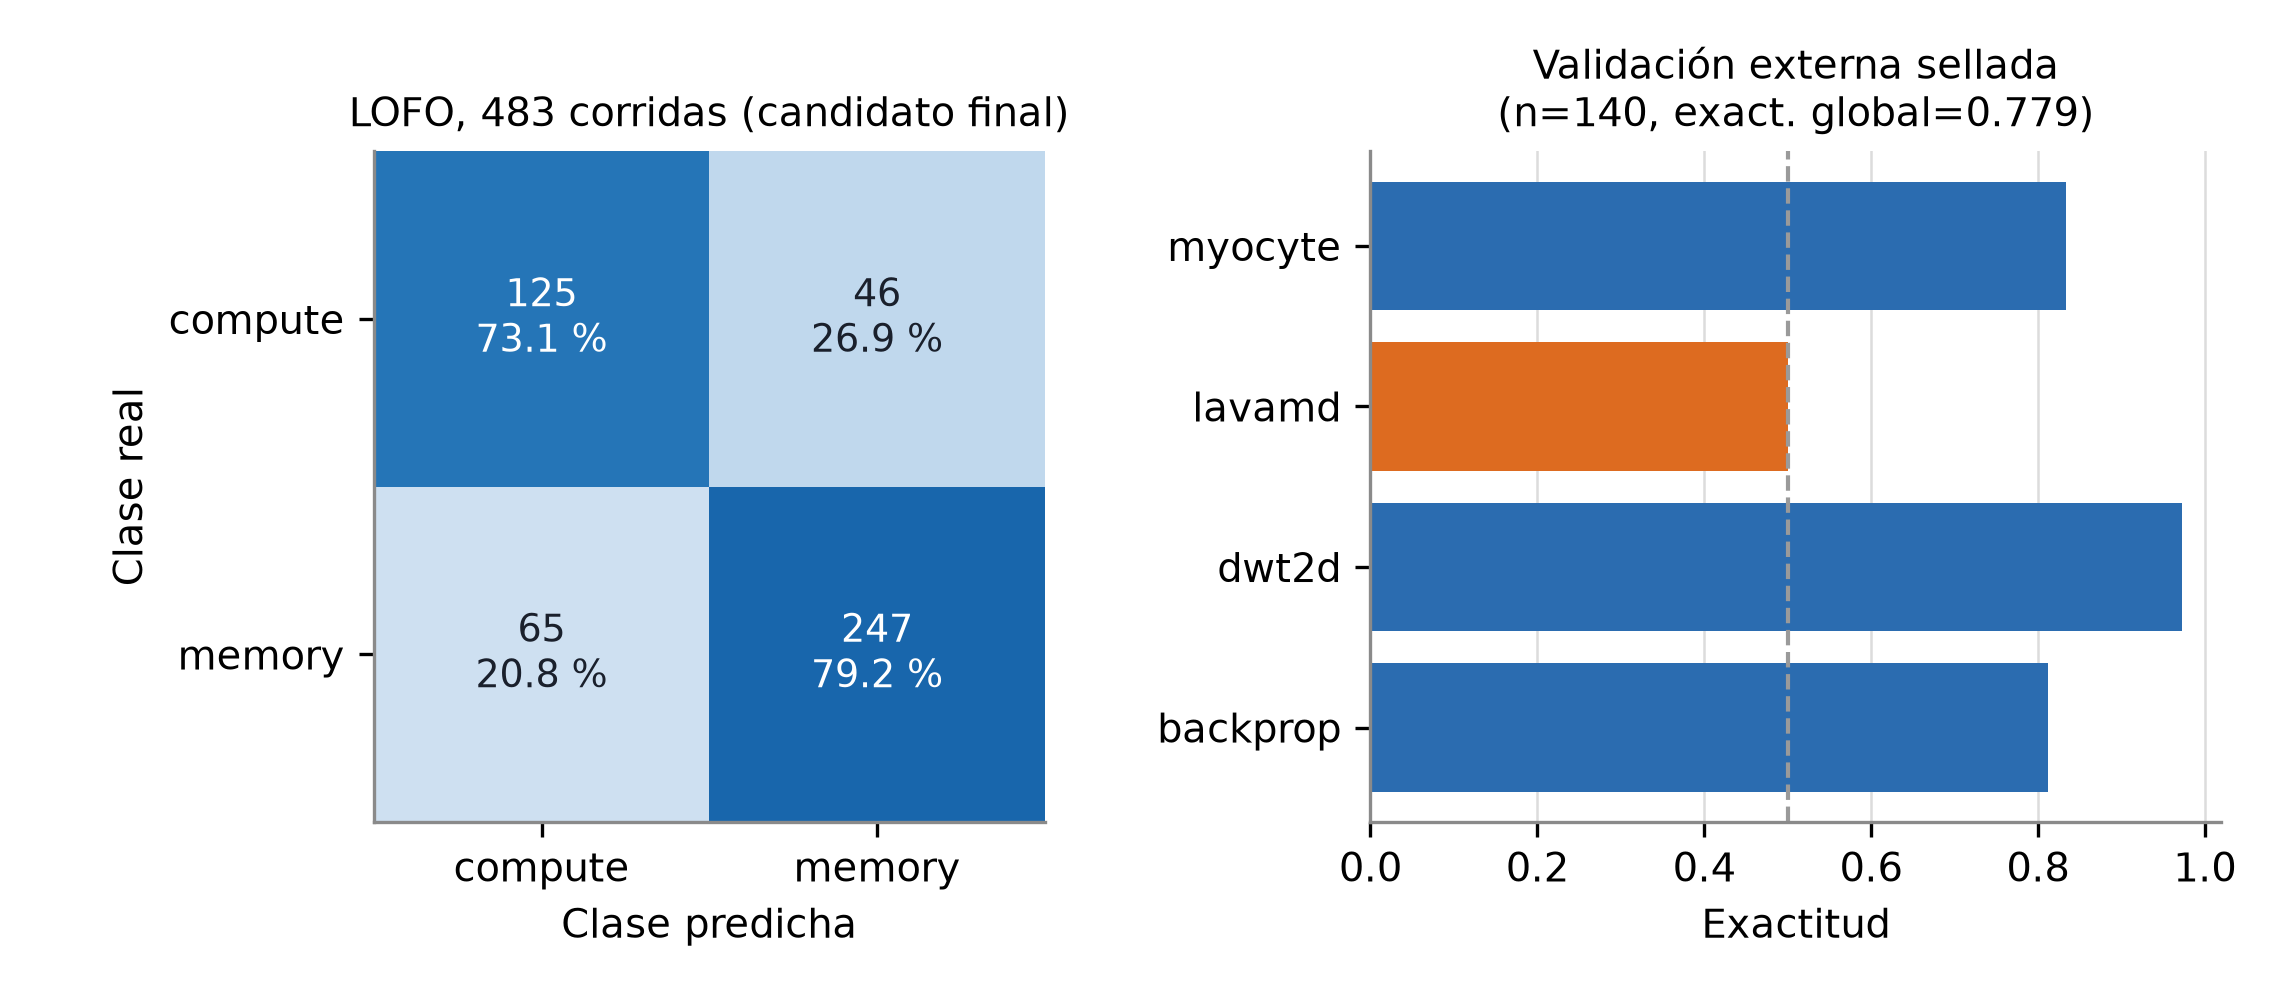
\includegraphics[width=\textwidth]{figuras/fig_gpu_matriz_confusion_20260922.png}
    \caption[Matriz de confusión y validación externa de la referencia estática GPU]{Izquierda, matriz de confusión agregada de la regresión logística de cinco entradas bajo \textit{leave-one-familia-out} (483 corridas). Derecha, exactitud por familia en la validación externa sellada (Backprop, DWT2D, LavaMD, Myocyte; 140 corridas nunca usadas en ninguna decisión de esta ronda). Fuente: elaboración propia.}
    \label{fig:gpu-matriz-confusion}
\end{figure}



\subsection{Candidato operativo de GPU: invarianza frente a la acción del agente}
\label{sec:resultados-gpu-invarianza}

La regresión logística de la subsección anterior es la referencia estática más rápida, pero el agente exige además que sus entradas no dependan del reloj que él mismo fija (sección \ref{sec:metodologia-invarianza-gpu}). La auditoría, sobre las mismas 483 corridas y sin mediciones nuevas, muestra que ese requisito cambia el modelo seleccionado (Figura \ref{fig:gpu-invarianza}). Al fijar de forma contrafactual el reloj de cada observación en 1410~MHz, la regresión logística cambia de clase el 26.7\% de sus predicciones, y su exactitud baja de 0.792 a 0.654 al excluir el reloj. El \textit{random forest} conserva el desempeño al retirar las entradas afectadas por la actuación, con 0.807 usando cinco variables, 0.812 sin reloj y 0.819 sin reloj ni potencia.

\begin{figure}[H]
    \centering
    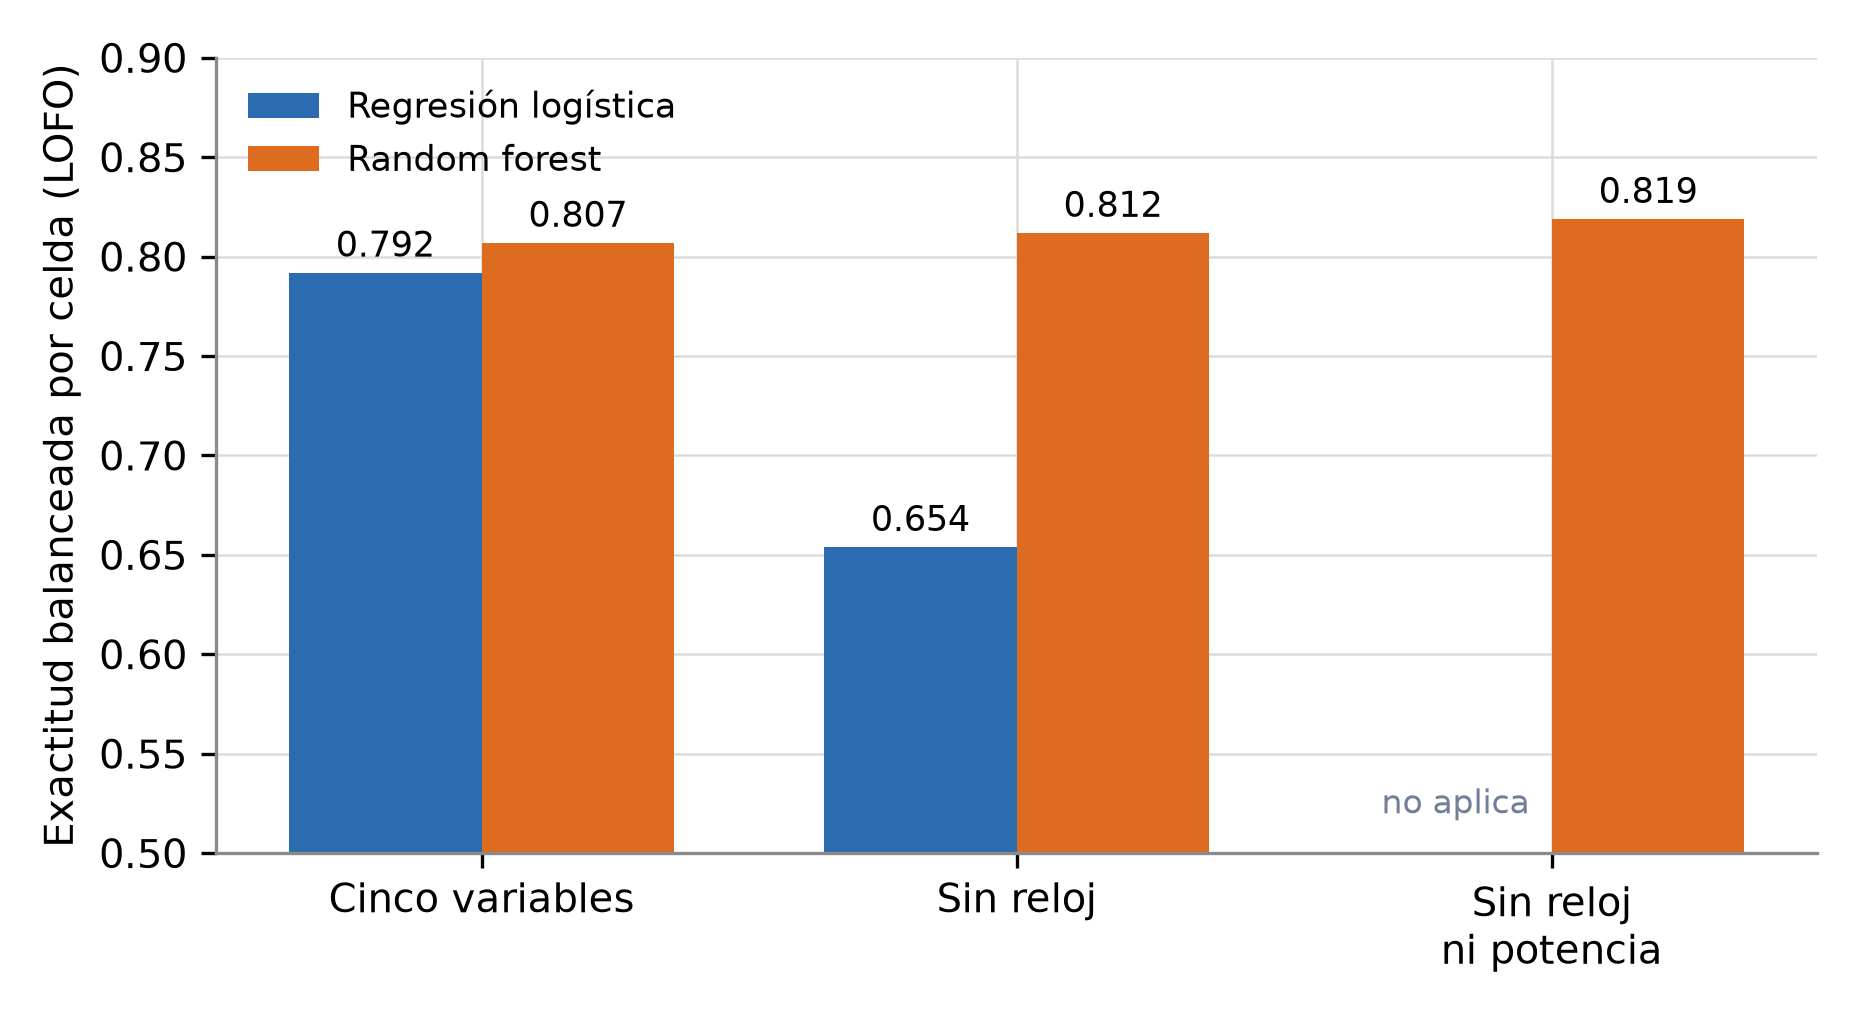
\includegraphics[width=0.85\textwidth]{figuras/fig_gpu_invarianza_reloj_20260923.png}
    \caption[Invarianza de los candidatos GPU frente al reloj]{Exactitud balanceada por celda (LOFO, 483 corridas, 16 familias) al excluir las variables que dependen de la acción del agente. Fuente: elaboración propia.}
    \label{fig:gpu-invarianza}
\end{figure}

El daemon consume el \textit{random forest} de tres entradas invariantes de la Tabla \ref{tab:gpu-modelos-operativos}. Su ECE LOFO es 0.0868 y su inferencia mediana tarda 4.7~ms, frente a los segundos requeridos para detectar y actuar sobre una fase. Con el umbral de 0.90 alcanza 0.900 de exactitud balanceada sobre el 65.7\% de las corridas aceptadas. El agente decide una sola vez por fase, por lo que una abstención no se reevalúa.

\begin{table}[H]
\centering
\caption{Modelos GPU después de aplicar el contrato de entradas del daemon. Las métricas se obtienen con LOFO sobre 483 corridas y 16 familias.}
\label{tab:gpu-modelos-operativos}
\small
\setlength{\tabcolsep}{3pt}
\begin{tabular}{@{}p{2.8cm}p{3.7cm}>{\centering\arraybackslash}p{2.1cm}>{\centering\arraybackslash}p{1.0cm}>{\centering\arraybackslash}p{1.7cm}@{}}
\toprule
\textbf{Modelo} & \textbf{Entradas} & \textbf{Exactitud balanceada} & \textbf{ECE} & \textbf{Estado} \\
\midrule
Regresión logística & Cinco señales NVML, incluidas potencia y reloj SM & 0.792 & 0.0569 & Referencia estática \\
\textit{Random forest} & Utilización GPU, utilización de memoria y desviación estándar de esta última & 0.819 & 0.0868 & Desplegado \\
\bottomrule
\end{tabular}
\end{table}

\subsection{Política de frecuencia por clase en GPU}
\label{sec:resultados-gpu-politica}

La tabla clase--frecuencia se derivó sobre las mismas 483 corridas de la sección anterior, con el kernel como unidad de comparación y el procedimiento de la sección \ref{sec:metodologia-politica-gpu}: mediana de repeticiones por kernel y nivel, prueba pareada contra \texttt{REF} e intervalo de confianza del 95\% por \textit{bootstrap}. Un cálculo preliminar emparejó en cambio, kernel por kernel, sus tres repeticiones de cada nivel contra sus tres de \texttt{REF} ($n=3$ por prueba); se descartó por responder una pregunta distinta de la que decide la tabla --- si el ruido de medición dentro de un kernel es distinguible de cero, no si el efecto generaliza entre kernels --- y se sustituye aquí por el resultado con el kernel, y su agregación por familia, como unidad.

De los 19 kernels con corridas aceptadas, uno (\texttt{minibude\_cuda\_bm1}) queda fuera por no tener más que una repetición en un solo nivel. De los 18 restantes, cuatro --- el núcleo GEMM y el \textit{stencil} de calor de RAJAPerf, y las variantes de menor tamaño de \texttt{dual\_axpy} y \texttt{dual\_stencil} --- quedan fuera de la prueba por no tener corridas en \texttt{REF} bajo la rejilla disponible, no por decisión editorial: sin \texttt{REF} no hay con qué parear. Restan 5 kernels \textit{compute\_bound} y 9 \textit{memory\_bound}, de los cuales tres pares (\texttt{dual\_axpy}, \texttt{dual\_spmv} y \texttt{dual\_stencil}, en su variante con \texttt{REF}) son el mismo algoritmo en dos tamaños de problema; la Tabla \ref{tab:gpu-politica-ic} agrega esos pares dentro de su familia (8 familias \textit{memory\_bound}, 5 \textit{compute\_bound}), con validación \textit{leave-one-familia-out} de la regla de nivel elegido.

\begin{table}[H]
\centering
\caption{Síntesis de la política GPU. Las ganancias son de EDP frente a REF; la rejilla completa se conserva en la Tabla \ref{tab:gpu-politica-detalle} del Anexo \ref{anexo:resultados-complementarios}.}
\label{tab:gpu-politica-ic}
\small
\begin{tabular}{@{}p{2.5cm}p{7.7cm}p{3.1cm}@{}}
\toprule
\textbf{Clase} & \textbf{Evidencia decisiva} & \textbf{Política} \\
\midrule
Cómputo & F1: $+2.1\%$ (IC95 $[-12.7;14.2]$, $p=0.438$); sin mejora confiable & No actuar \\
Memoria & F1: $+8.9\%$ (IC95 $[3.0;13.3]$, $p=0.020$); siete de ocho familias mejoran & Fijar F1 \\
\bottomrule
\end{tabular}
\end{table}



El resultado es \textbf{no actuar} en \textit{compute\_bound} y \textbf{actuar en F1 para \textit{memory\_bound}} (Figura \ref{fig:gpu-politica-forest}), con una ganancia agregada de 8.9\% (IC95 de 3.0 a 13.3\%, $p=0.020$, 7 de 8 familias mejoran). La validación \textit{leave-one-familia-out} --- aplicar la regla ``elegir F1'' a cada familia excluida, usando solo las siete restantes para elegirla --- confirma la dirección: siete de ocho pliegues eligen F1 de forma independiente y la ganancia realizada fuera de muestra es 6.5\% (IC95 de $-4.0$ a 13.1\%, un intervalo que roza cero por tratarse de solo ocho familias, pero consistente en signo con el resultado de la Tabla \ref{tab:gpu-politica-ic}). F2 muestra una ganancia de magnitud similar (7.4\%) pero no alcanza significancia con la familia como unidad, a diferencia del resultado preliminar por kernel: la diferencia es exactamente el efecto de dejar de contar dos veces los mismos algoritmos en dos tamaños.

\begin{figure}[H]
    \centering
    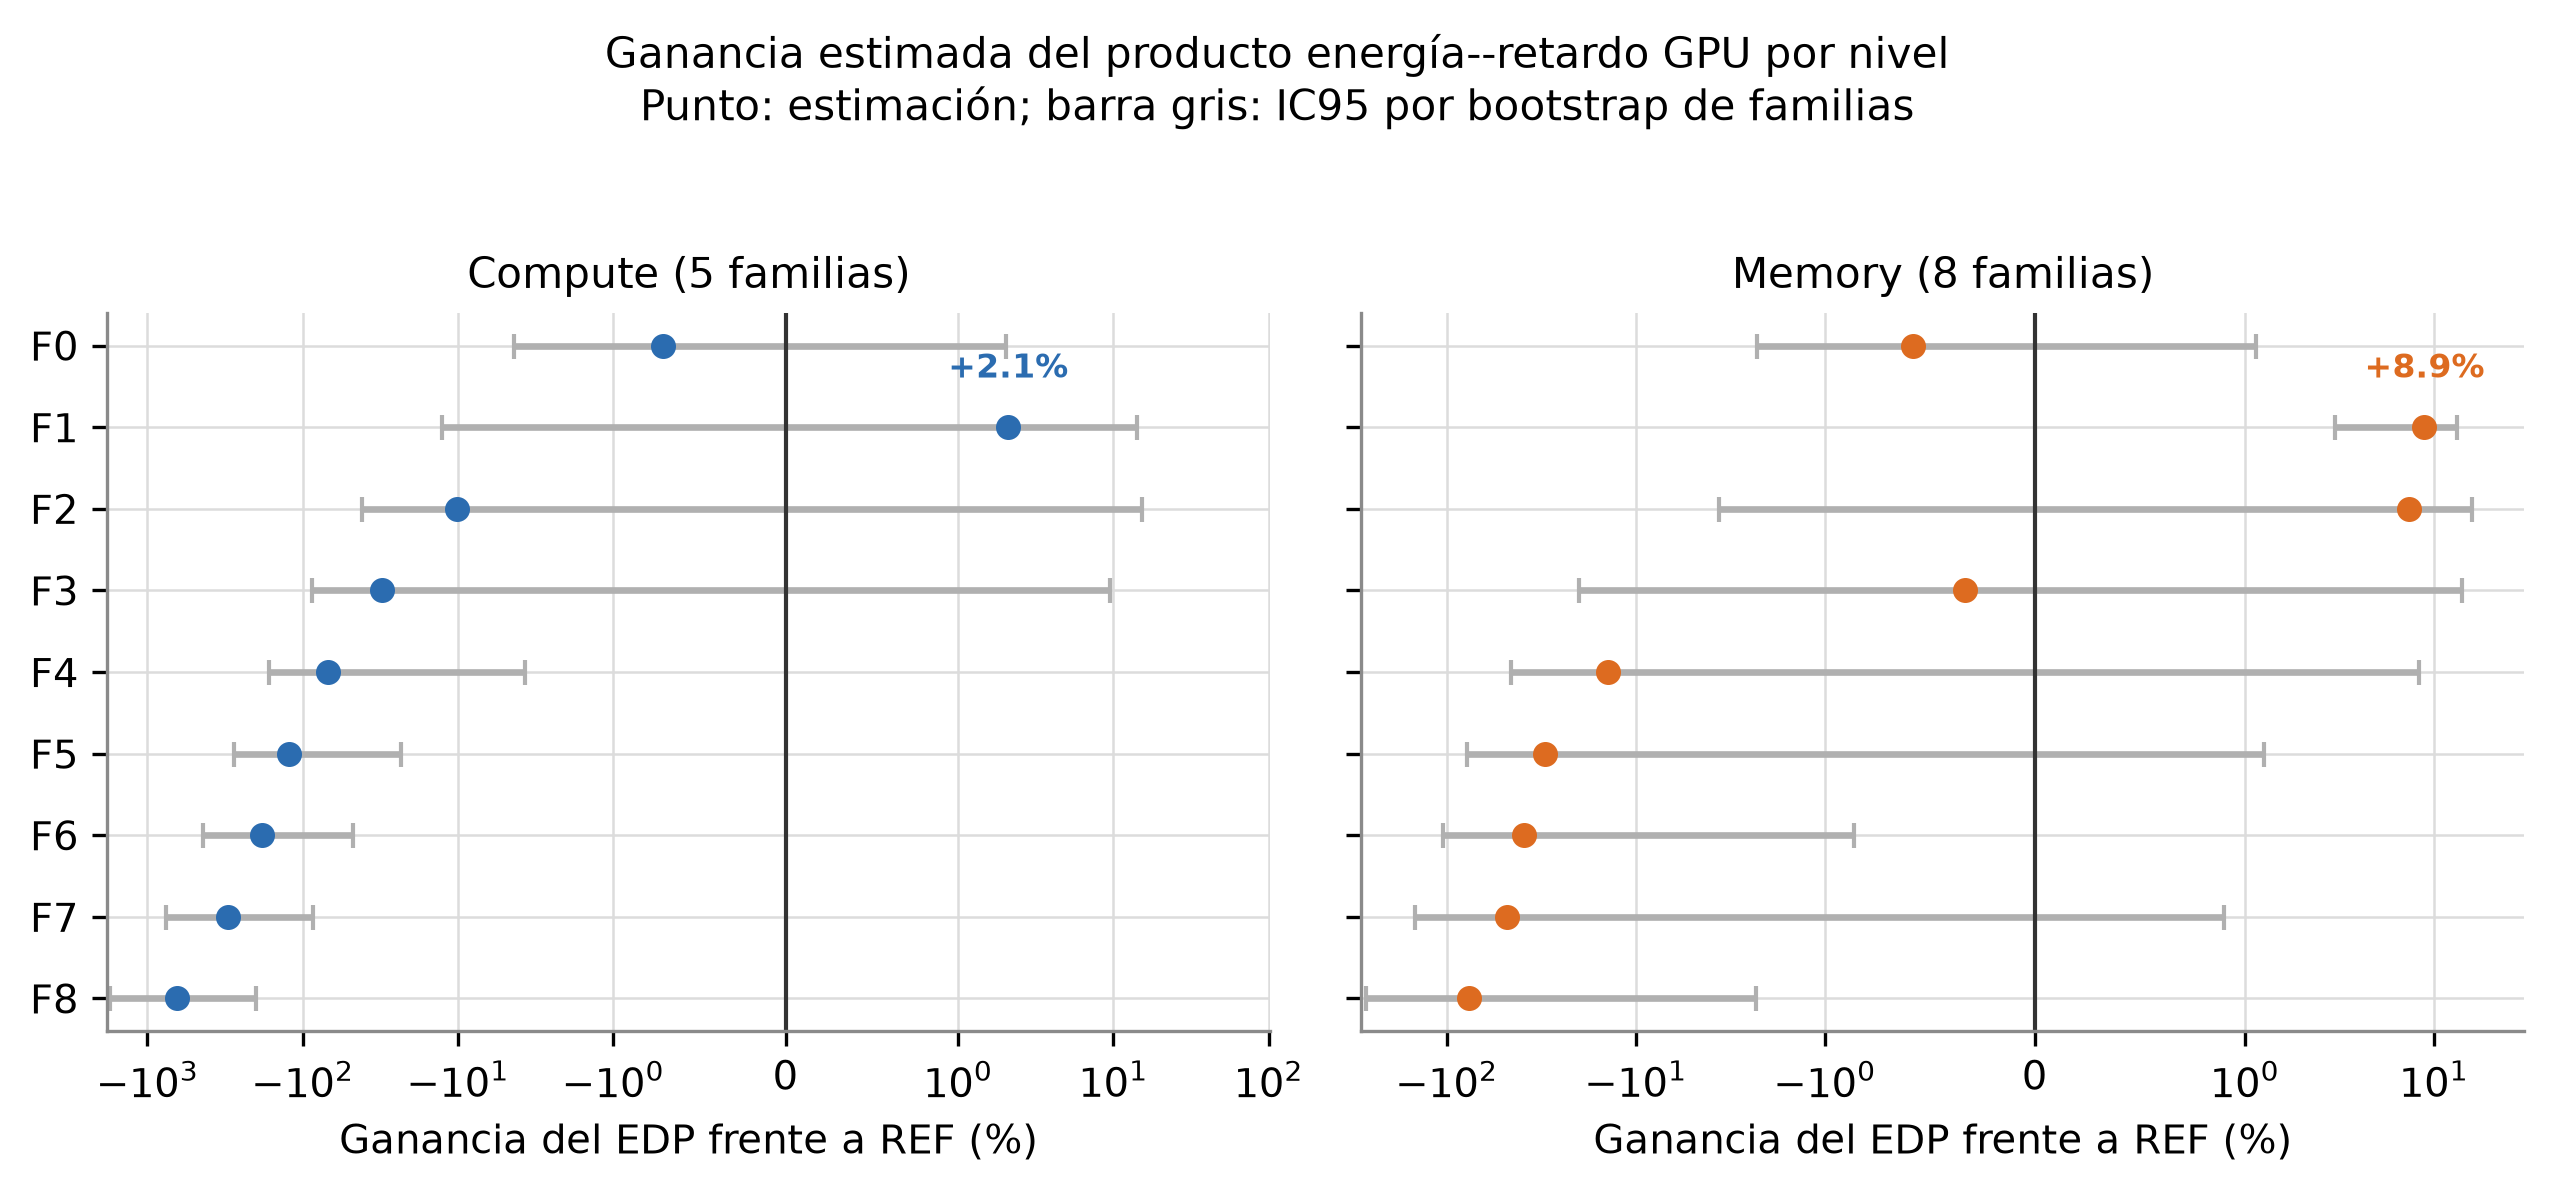
\includegraphics[width=0.94\textwidth]{figuras/fig_gpu_politica_forest_20260922.png}
    \caption[Ganancia del EDP GPU por nivel y clase, en forma de \textit{forest plot}]{La rejilla completa de la Tabla \ref{tab:gpu-politica-detalle}, en forma gráfica, con la familia como unidad. Cada punto es la ganancia estimada y la barra gris, su IC95 por \textit{bootstrap}; los rótulos señalan F1. El eje horizontal es simétrico-logarítmico para mostrar a la vez F1, cercano a cero, y F8, con pérdidas de más de un orden de magnitud en \textit{compute\_bound}. Fuente: elaboración propia.}
    \label{fig:gpu-politica-forest}
\end{figure}

En \textit{compute\_bound}, F1 parece favorable en el promedio descriptivo (+2.1\%), pero su IC95 va de $-12.7\%$ a $+14.2\%$ y la prueba pareada da $p=0.438$. No constituye una mejora confiable. Además, la validación LOFO de la regla que escoge F1 produce una ganancia realizada de $-4.8\%$ (IC95 de $-13.4$ a $0\%$): al aplicarla a una familia que no participó en elegir el nivel, empeora en promedio. Por ello el daemon conserva REF en \textit{compute\_bound}; la conclusión coincide con la de CPU.

La pendiente mediana de sensibilidad del tiempo al reloj SM es 0.837 en cómputo ($n=6$) y 0.189 en memoria ($n=12$). Por ello, en memoria puede bajarse el reloj de cómputo sin prolongar proporcionalmente la espera por el dominio de memoria, que no se varió en la campaña. La excepción es \texttt{rodinia\_gaussian}, etiquetada como memoria pero con una pendiente de 0.941 (véase el desglose en el Anexo \ref{anexo:resultados-complementarios}).

La Figura \ref{fig:gpu-politica-energia-relativa} hace visible el mismo contraste: en \textit{compute\_bound} el tiempo y el EDP crecen juntos desde F1, porque la energía apenas cae; en \textit{memory\_bound} el tiempo crece mucho más lentamente y la energía sí cae de forma sostenida hasta F3, de modo que el EDP se mantiene por debajo de 1 en F1--F2 antes de que la caída de energía se agote y el tiempo tome el control a partir de F5. Ajustando $P(f)=P_0+c\,f^{k}$ a la potencia de cada kernel frente al reloj SM --- descartando seis de los 18 kernels cuyo rango de reloj disponible (menos de siete niveles con datos) o cuyo ajuste resultante ($R^2<0.8$) no identifica los tres parámetros de forma confiable ---, el piso estático $P_0$ resulta de 38.5~W en mediana sobre los 12 kernels restantes, y representa el 55.8\% de la potencia al reloj más alto (Figura \ref{fig:gpu-politica-piso}): un margen de potencia dinámica más amplio, proporcionalmente, que el 84\% estático de CPU, consistente con que \textit{memory\_bound} sí encuentre una región de mejora que CPU no encontró en ninguna clase.

\begin{figure}[H]
    \centering
    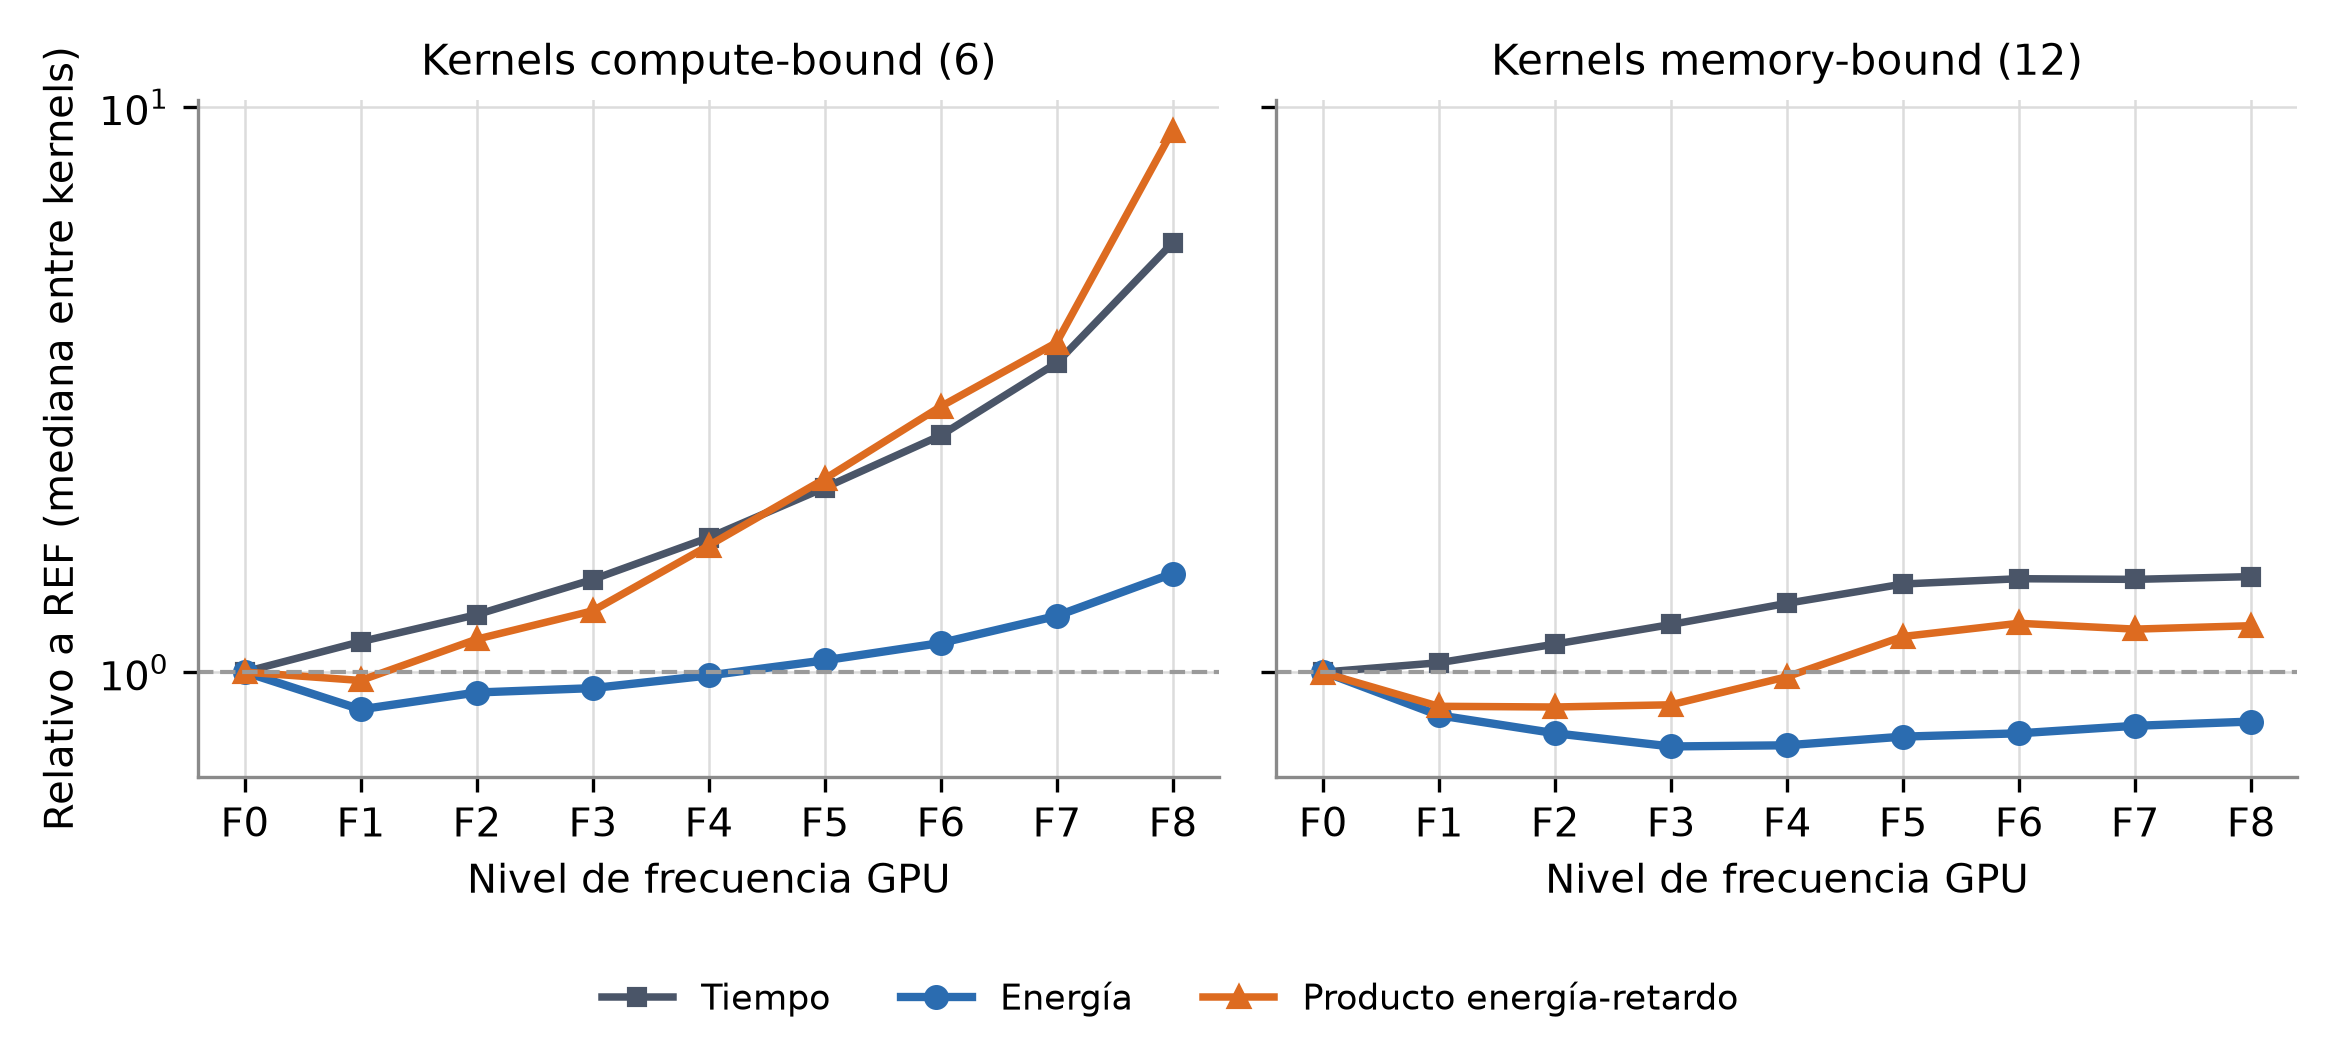
\includegraphics[width=0.94\textwidth]{figuras/fig_gpu_politica_energia_relativa_20260922.png}
    \caption[Tiempo, energía y EDP relativos por nivel de frecuencia GPU]{Mediana entre kernels del tiempo, la energía y el producto energía--retardo de cada nivel, relativos a \texttt{REF}, para las dos clases (5 y 9 kernels con corridas en \texttt{REF}, kernel como unidad, descriptivo; la significancia se evalúa por familia en la Tabla \ref{tab:gpu-politica-ic}). El eje vertical es logarítmico. Fuente: elaboración propia.}
    \label{fig:gpu-politica-energia-relativa}
\end{figure}

\begin{figure}[H]
    \centering
    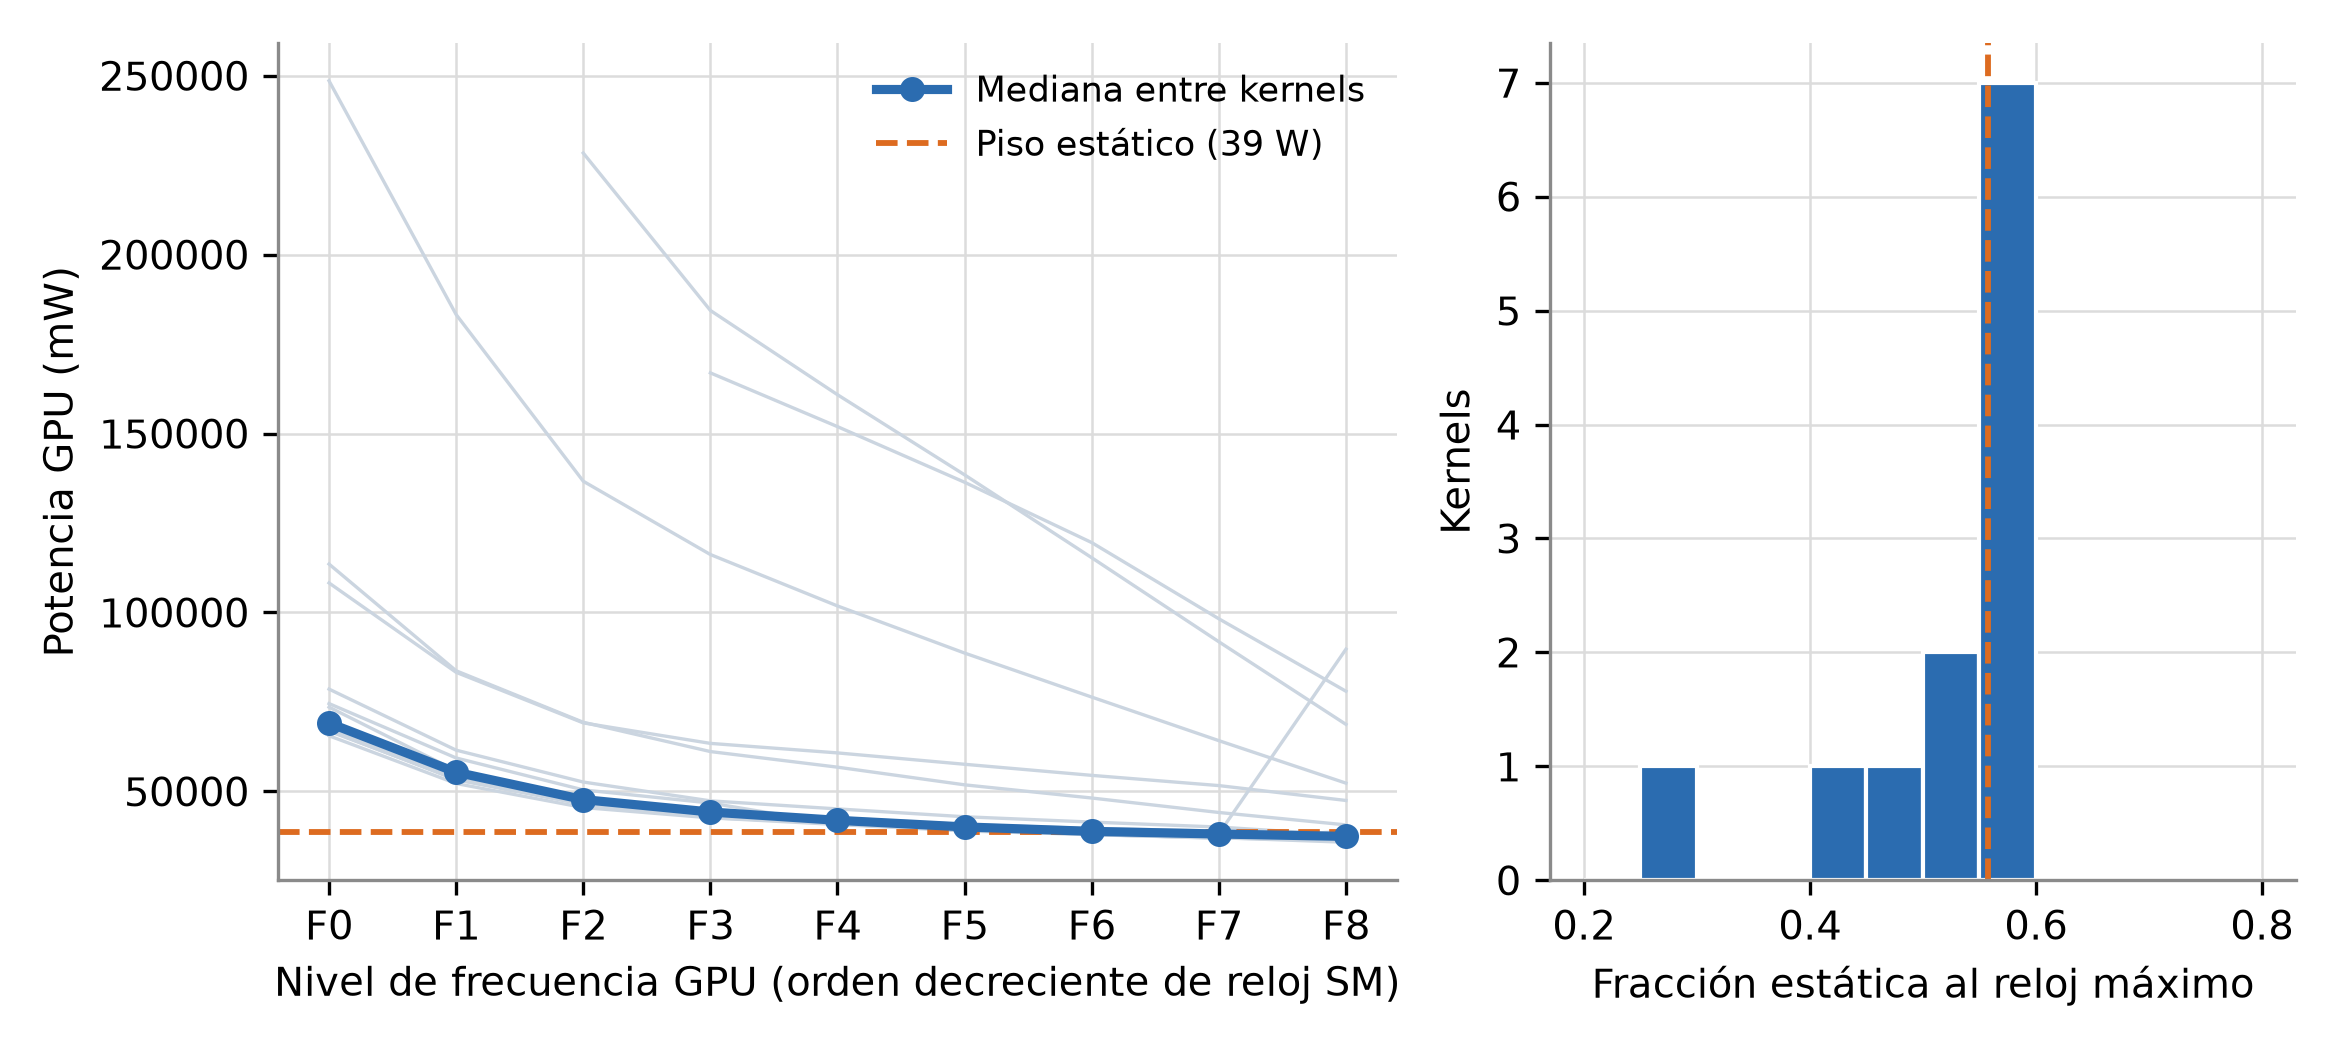
\includegraphics[width=0.94\textwidth]{figuras/fig_gpu_politica_piso_20260922.png}
    \caption[Potencia de GPU frente al reloj SM y piso estático]{Izquierda: potencia media de GPU de cada kernel (líneas grises) y su mediana en cada nivel, con el piso estático ajustado (12 kernels con ajuste identificable). Derecha: distribución entre esos kernels de la fracción de la potencia al reloj más alto que corresponde al piso. Fuente: elaboración propia.}
    \label{fig:gpu-politica-piso}
\end{figure}

En la validación por familia retirada, siete de ocho familias de memoria realizaron ganancias de 4.2 a 14.8\%; \texttt{rodinia\_gaussian} perdió 27.3\%. Su tiempo responde al reloj como una carga de cómputo pese a su etiqueta de memoria. Se conservó en el análisis: excluirla después de observar la pérdida sesgaría la política.

\subsection{Continuidad de la ruta CUPTI}
\label{sec:resultados-gpu-hiperparam}

La limitación observada en el reanálisis no invalida el uso de NVML como proxy ligero, pero delimita lo que puede esperarse de él. NVML mide efectos agregados de toda la GPU y no expone FLOPs, bytes movidos, ocupación ni la identidad del kernel activo en cada instante. Un sondeo más frecuente produce más lecturas del mismo estado agregado, no reconstruye los límites de los lanzamientos. Por ello se implementó una vía independiente, basada en la API de actividades de CUPTI, para ubicar en el tiempo real cada lanzamiento CUDA de una corrida y combinarlo con un modelo analítico de trabajo por lanzamiento \cite{CUPTI2026}. La biblioteca de captura se inyecta en el proceso CUDA medido, no en el proceso recolector, porque el lanzador separa ambos con \texttt{fork}+\texttt{exec}. Una auditoría de cobertura, de tipo \textit{fail-closed}, exige que todo kernel GPU del catálogo tenga registrado un modelo analítico de FLOPs y bytes por lanzamiento antes de permitir que una campaña con esta traza comience; diecinueve kernels del catálogo lo tienen.

Con esa infraestructura se ejecutó una campaña sobre el catálogo GPU completo, 544 corridas planificadas. La captura de la traza fue correcta: la corrida de \textit{rodinia\_gaussian} registró 8197 eventos CUPTI, consistentes con los aproximadamente 8190 lanzamientos esperados de \texttt{Fan1}/\texttt{Fan2} para una eliminación gaussiana de tamaño 4096. El mecanismo de captura por lanzamiento funciona como fue diseñado.

La campaña CUPTI capturó los lanzamientos, pero su eje de frecuencia no fue válido: con solicitudes de 700 y 1200~MHz, el reloj observado permaneció en 765~MHz. Ninguna ventana cumplió la tolerancia de reloj para entrenar por nivel. Se conservaron las trazas y calibraciones; una verificación posterior volvió a encontrar operativo el candado (sección \ref{sec:resultados-agente-candado}). Por tanto, el fallo afecta esa campaña, no la política GPU derivada de las 483 corridas previas.

CUPTI mantiene dos funciones futuras diferenciadas, independientes del resultado anterior. Su perfilado de contadores puede construir una intensidad operacional y una etiqueta Roofline por kernel en una campaña controlada. Su API de actividades, ya implementada, puede registrar los límites temporales de lanzamientos y transferencias necesarios para asociar esa etiqueta con el segmento NVML de la misma fase. La granularidad fina requiere ambas fuentes en la misma campaña: sin el perfilado no se conoce la clase física de cada fase, y sin la traza no se sabe qué parte de la telemetría corresponde a esa fase. Ninguna de estas funciones convierte automáticamente a CUPTI en una entrada del clasificador en producción, que debe conservar únicamente señales ligeras de NVML. La reconstrucción del eje de frecuencia de esa campaña y una nueva evaluación de etiquetas por fase con CUPTI quedan como extensiones; la política de frecuencia GPU de este trabajo se obtuvo de la campaña anterior válida.

\section{Resultados del agente de control}
\label{sec:resultados-agente}

Esta sección reporta la verificación del agente de la Fase 3 en \texttt{paccaA100}, antes de la evaluación de la Fase 4. Todas las pruebas usaron el nodo en asignación exclusiva y restauraron el estado de frecuencia al terminar.

\subsection{Candado de reloj de GPU y premisa física de la política}
\label{sec:resultados-agente-candado}

Con una carga sintética de fases controladas se comprobó que, al fijar el reloj con \texttt{nvidia-smi -lgc}, el reloj observado coincide con el solicitado en los seis valores probados (1410, 1260, 1110, 810, 510 y 210~MHz), y que el rendimiento responde con la forma que supone la política (Figura \ref{fig:agente-candado}): el de una carga \textit{compute\_bound} escala aproximadamente con el reloj, mientras que el de una carga \textit{memory\_bound} no cae hasta llegar a 510~MHz. Es la premisa física de bajar el reloj en la clase \textit{memory\_bound} sin costo de tiempo, medida sobre el mismo instrumento que aplicará el agente.

\begin{figure}[H]
    \centering
    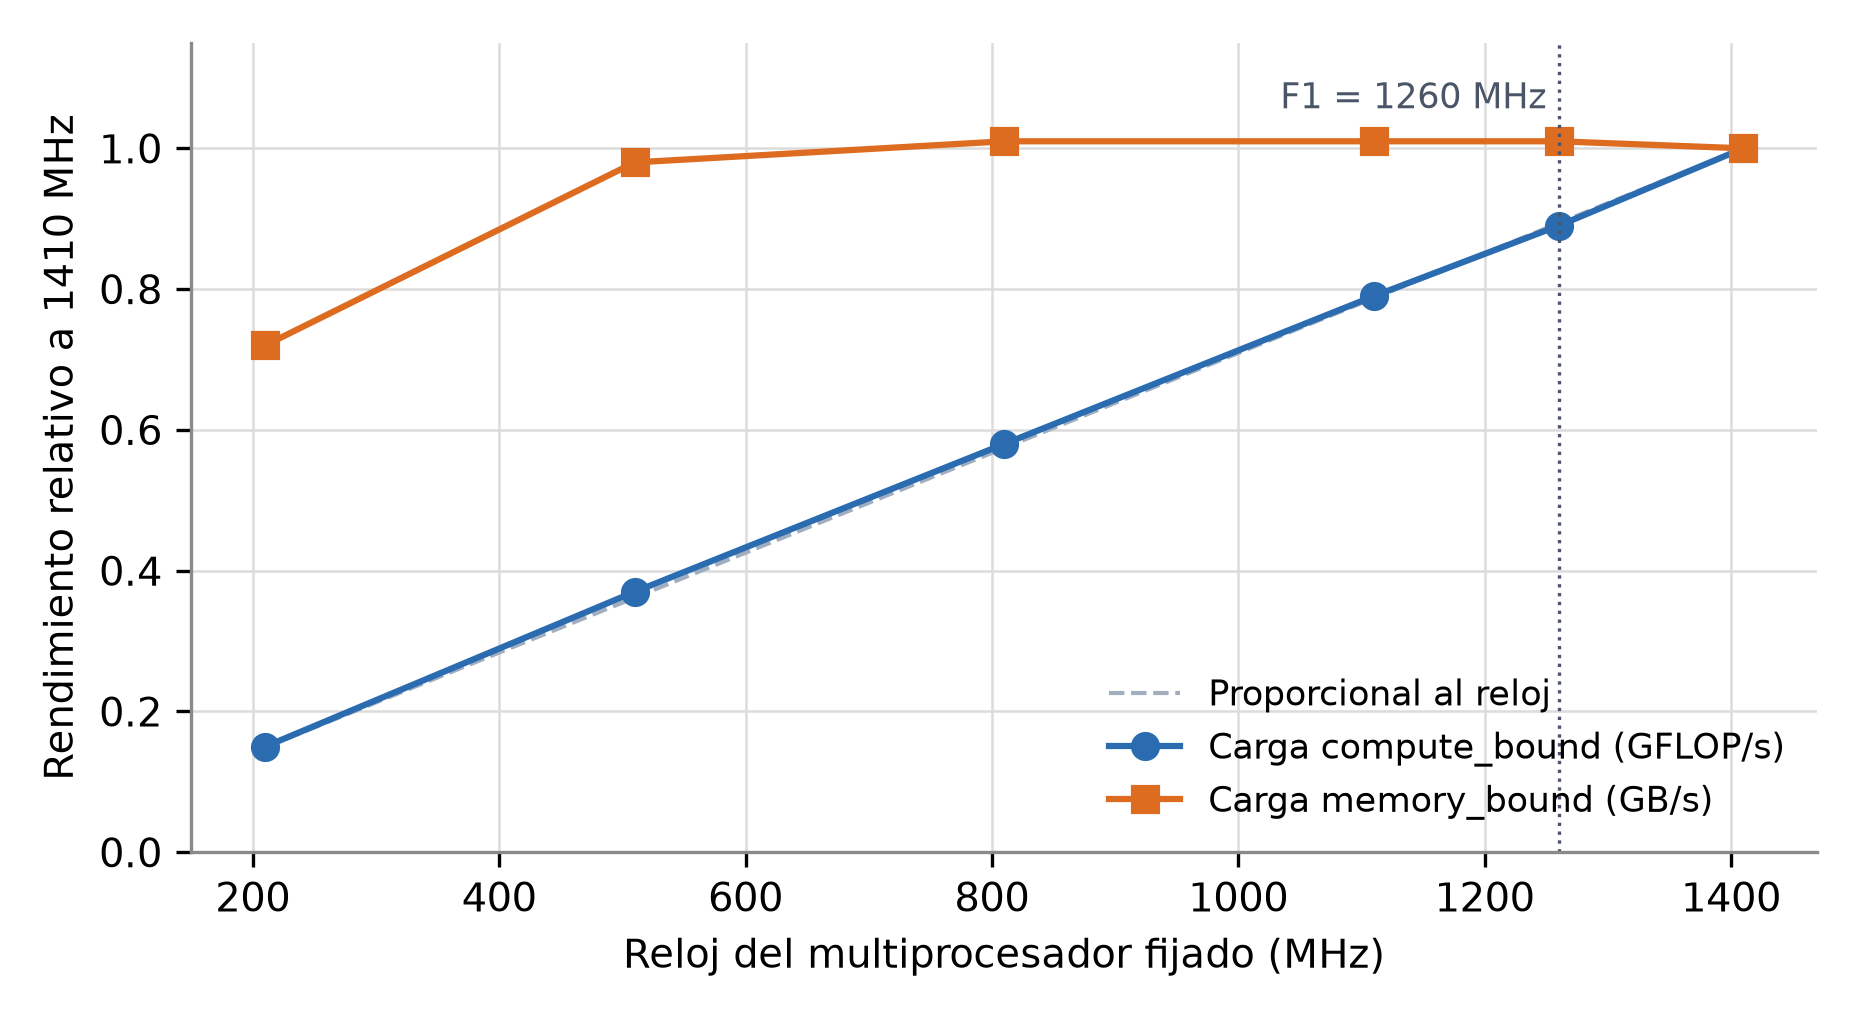
\includegraphics[width=0.85\textwidth]{figuras/fig_gpu_candado_rendimiento_20260923.png}
    \caption[Rendimiento de GPU con el reloj fijado]{Rendimiento relativo al reloj de 1410~MHz con el reloj de GPU fijado, para una carga \textit{compute\_bound} y una \textit{memory\_bound}; la línea discontinua es la proporcionalidad exacta al reloj. Fuente: elaboración propia.}
    \label{fig:agente-candado}
\end{figure}

\subsection{Latencias de conmutación y sobrecarga}
\label{sec:resultados-agente-latencias}

La Tabla \ref{tab:agente-latencias} resume las latencias de conmutación y la sobrecarga de cada proceso. La permanencia mínima entre cambios de reloj en GPU se fijó en 10 veces la latencia de conmutación observada, es decir, 3.7~s. La sobrecarga en energía de paquete del brazo \textit{sombra} frente al \textit{base} se mide en la Fase 4.

\begin{table}[H]
\centering
\caption{Latencias de conmutación y sobrecarga del agente en \texttt{paccaA100}.}
\label{tab:agente-latencias}
\small
\setlength{\tabcolsep}{3pt}
\begin{tabular}{@{}>{\raggedright\arraybackslash}p{1.6cm}>{\raggedright\arraybackslash}p{8.5cm}>{\centering\arraybackslash}p{3.0cm}@{}}
\toprule
\textbf{Dispositivo} & \textbf{Magnitud} & \textbf{Valor} \\
\midrule
GPU & Comando de fijado de reloj & $\approx$ 50~ms \\
GPU & Reloj observado en el valor pedido (tras el comando) & 70 a 80~ms \\
GPU & Uso de CPU del proceso con la GPU en reposo & 0.0 a 0.1\% de un núcleo \\
CPU & Escritura secuencial de límites en los núcleos delegados & 27.9~ms \\
CPU & Escritura en paralelo, un hilo por núcleo & 2.85~ms \\
CPU & Inferencia del clasificador (percentil 50 / 99) & 16.4 / 19.3~$\mu$s \\
\bottomrule
\end{tabular}
\end{table}

\subsection{Restauración bajo terminación anómala y coordinación}
\label{sec:resultados-agente-restauracion}

La Tabla \ref{tab:agente-restauracion} resume las pruebas de restauración y de coordinación. En cada prueba de terminación anómala inducida (\texttt{SIGTERM} o \texttt{SIGINT}) el agente atendió la señal y devolvió el dispositivo a su estado inicial, con código de salida 0. La prueba de coexistencia ejecutó ambos procesos en brazo activo sobre la aplicación compuesta A de GPU con el piso de CPU en 3.2~GHz.

\subsection{Detección y clasificación de fase de GPU sobre aplicaciones compuestas}
\label{sec:resultados-agente-deteccion}

La Tabla \ref{tab:agente-deteccion} reporta la clasificación de fase de GPU del agente sobre las dos aplicaciones compuestas, con el umbral de abstención de 0.90. En la aplicación A, las decisiones correctas tuvieron confianza 1.00 y las abstenciones entre 0.57 y 0.67; en la aplicación B, \textit{LavaMD}, una familia inédita, se clasificó correctamente con confianza 1.00. Los conteos son pequeños y sirven para verificar el funcionamiento del detector y de la abstención; la exactitud con muestra suficiente es lo que mide la Fase 4.



\section{Evaluación del agente frente a REF (Fase 4)}
\label{sec:resultados-fase4}

Esta sección reporta la evaluación experimental del agente frente al \textit{governor} nativo con turbo (REF) en \texttt{paccaA100}, según la matriz de la sección \ref{sec:metodologia-fase4}. Se reportan la matriz inicial (escenario A), sus repeticiones de comprobación, los escenarios C, D y E, el confirmatorio de E-A, CloverLeaf y la línea base secundaria sin turbo. Las razones de las tablas se calculan sobre la mediana de cada brazo y se expresan frente a la mediana de REF de la misma combinación experimental; un valor menor que 1 es una mejora. Cuando el diseño usa bloques, también se reportan las razones emparejadas por bloque.

\subsection{Aplicaciones compuestas}
\label{sec:resultados-fase4-apps}

Cada alcance usa dos aplicaciones compuestas que encadenan kernels del catálogo, con la clase de cada fase conocida de antemano. La aplicación A reúne familias vistas durante el entrenamiento y la B familias inéditas. La Figura \ref{fig:fase4-aplicaciones} muestra la estructura de un ciclo y la Tabla \ref{tab:fase4-apps} el detalle por kernel. La fracción de tiempo en fases \textit{memory\_bound} varía entre 15\% (CPU, B) y 71\% (CPU, A), y es la magnitud que acota cuánto puede ahorrar cualquier política que solo actúe en esa clase.

\begin{figure}[H]
    \centering
    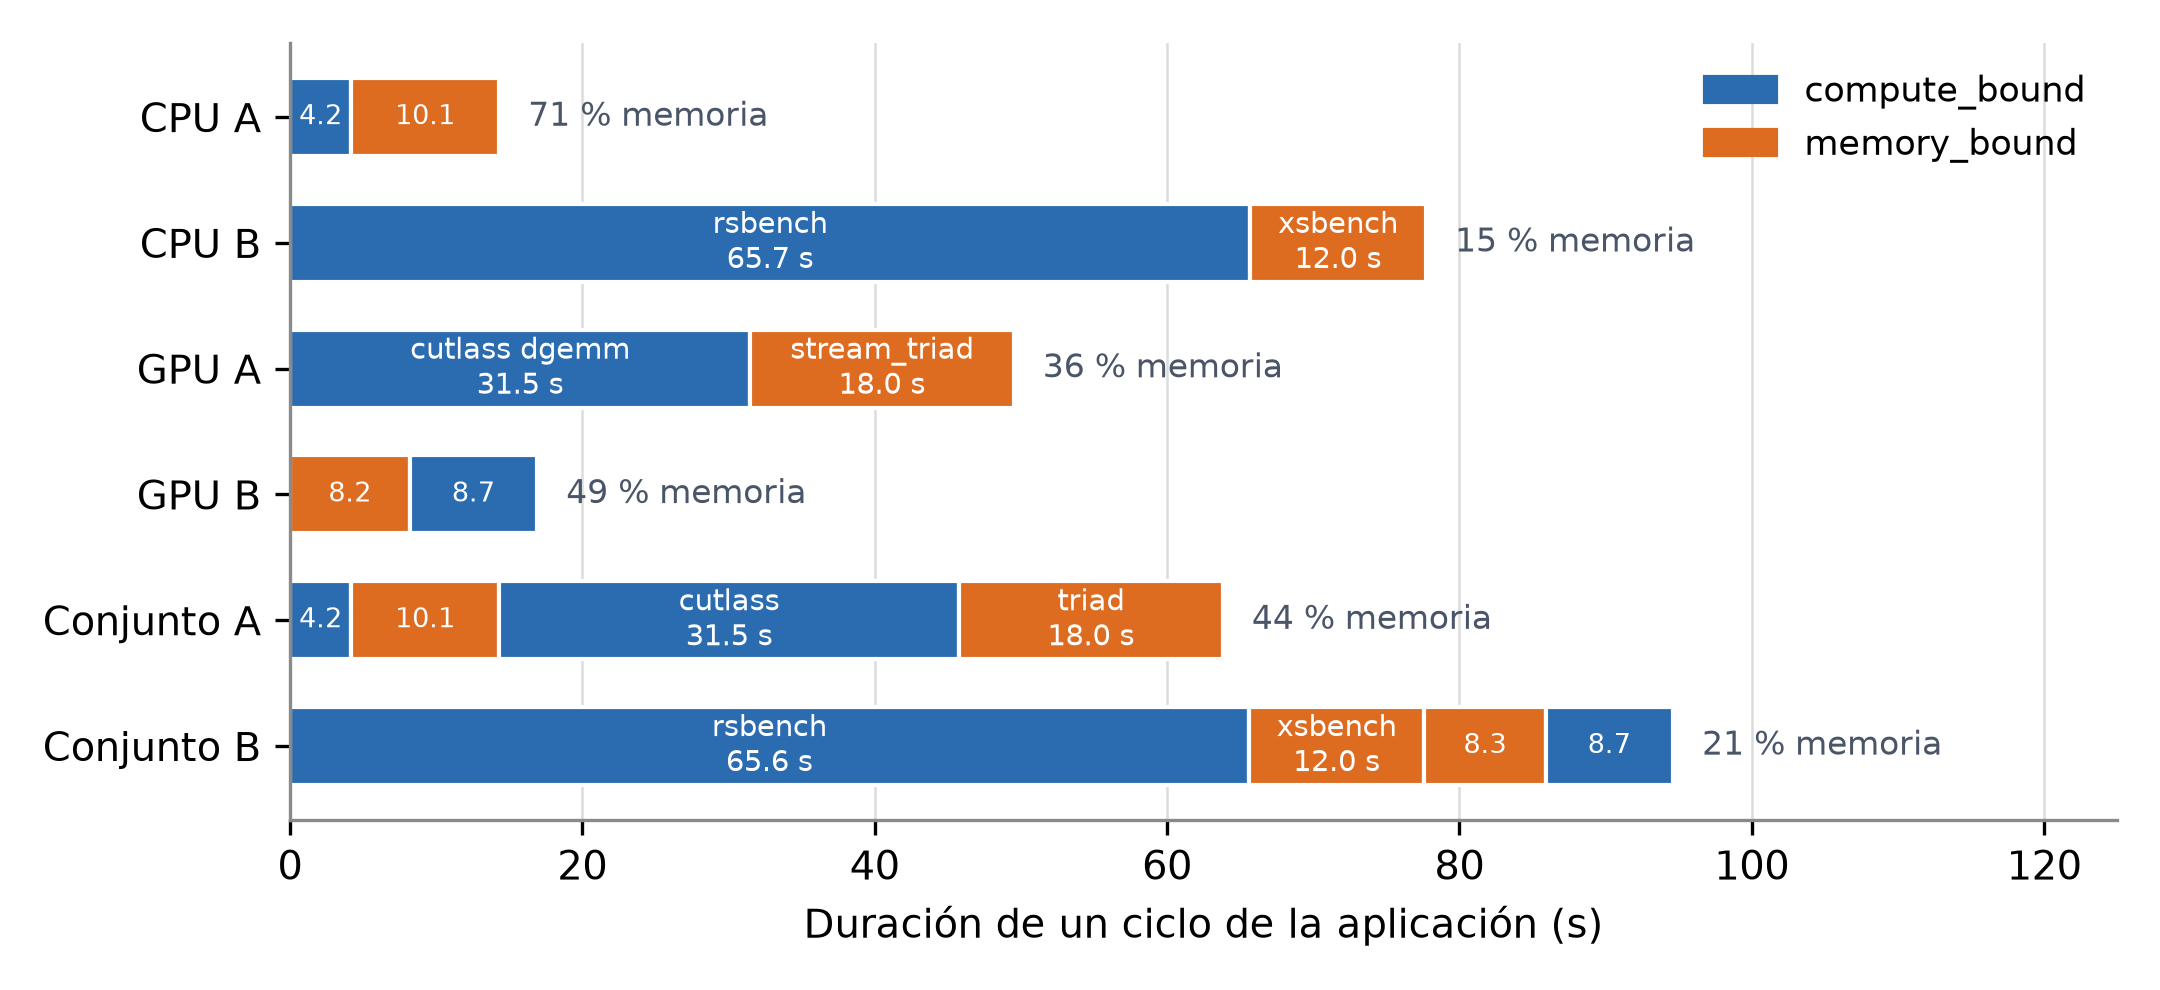
\includegraphics[width=0.94\textwidth]{figuras/fig_fase4_aplicaciones_20260924.png}
    \caption{Estructura de un ciclo de cada aplicación compuesta. Los números dentro de las barras son la duración media de cada fase en segundos; a la derecha, la fracción del ciclo en fases \textit{memory\_bound}.}
    \label{fig:fase4-aplicaciones}
\end{figure}



\subsection{Clasificación de fase con el agente en el lazo}
\label{sec:resultados-fase4-clasificacion}

La Tabla \ref{tab:fase4-clasificacion} puntúa cada decisión del agente contra la fase real en que cae su instante. En CPU las decisiones son por ventana de un milisegundo, de modo que hay decenas de miles por celda y la exactitud está ponderada por la duración de cada fase; en GPU hay una decisión por fase, con una permanencia mínima de 3.7~s.

En CPU, el agente acierta el 94\% de las decisiones sobre las familias vistas y más del 99.7\% sobre las inéditas. La diferencia favorable a las inéditas no debe leerse como mejor generalización: en la aplicación B una sola fase de cómputo ocupa el 85\% del tiempo y ponderar por ventanas la hace dominante, de modo que el resultado depende de cómo se separan esos dos kernels y no de familias arbitrarias. En GPU no hubo ninguna decisión errónea entre las que el agente tomó, pero se abstuvo con frecuencia: una de doce fases en A y entre cuatro y seis de doce en B (en el alcance conjunto, entre tres y siete de veinte). Toda fase, en cualquier alcance, recibió al menos una decisión. La exactitud del brazo activo y la del brazo sombra son indistinguibles, como corresponde a un clasificador cuya entrada no depende de la acción del agente.



\subsection{Tiempo, energía y EDP frente a REF}
\label{sec:resultados-fase4-edp}

La Tabla \ref{tab:fase4-resultados} y la Figura \ref{fig:fase4-edp} reportan la duración, las energías de CPU y de GPU por separado y las razones frente a REF de la matriz inicial. Tres hechos separan los alcances:

\begin{itemize}
    \item En \textbf{GPU} el agente activo no cambia el resultado: el EDP del nodo queda en 1.00 frente a REF en A y en B (y el brazo sombra, en 1.01 y 1.00). El agente de GPU no impone sobrecarga medible.
    \item En \textbf{CPU} el brazo activo queda entre 1.7 y 2.0 veces peor que REF en EDP, con un aumento de 15 a 25\% en tiempo y de 55 a 63\% en energía de CPU.
    \item En el alcance \textbf{conjunto} el EDP queda entre 1.3 (A) y 1.6 (B) veces el de REF. Con cinco repeticiones por brazo, la prueba de Mann--Whitney da $p = 0.0079$ en todas las comparaciones contra REF, que es el mínimo alcanzable con cinco contra cinco: las cinco corridas de cada brazo quedaron por encima de las de REF.
\end{itemize}

La descomposición por brazo indica dónde se origina la diferencia. El brazo sombra, que decide pero no escribe ninguna frecuencia, ya presenta prácticamente todo el exceso de CPU. La Tabla \ref{tab:fase4-activo-sombra} compara el brazo activo con el sombra: el efecto atribuible a la acción de frecuencia está entre $-3.3\%$ y $+2.9\%$ del EDP, es decir, de pocos puntos y de signo mixto (peor en CPU con kernels vistos, mejor con los inéditos y en el alcance conjunto). Poner F0 también en \textit{memory} (\textit{activo-F0}) o quitar el piso de coordinación (\textit{activo sin piso}) no cambia el resultado de forma apreciable.

\begin{figure}[H]
    \centering
    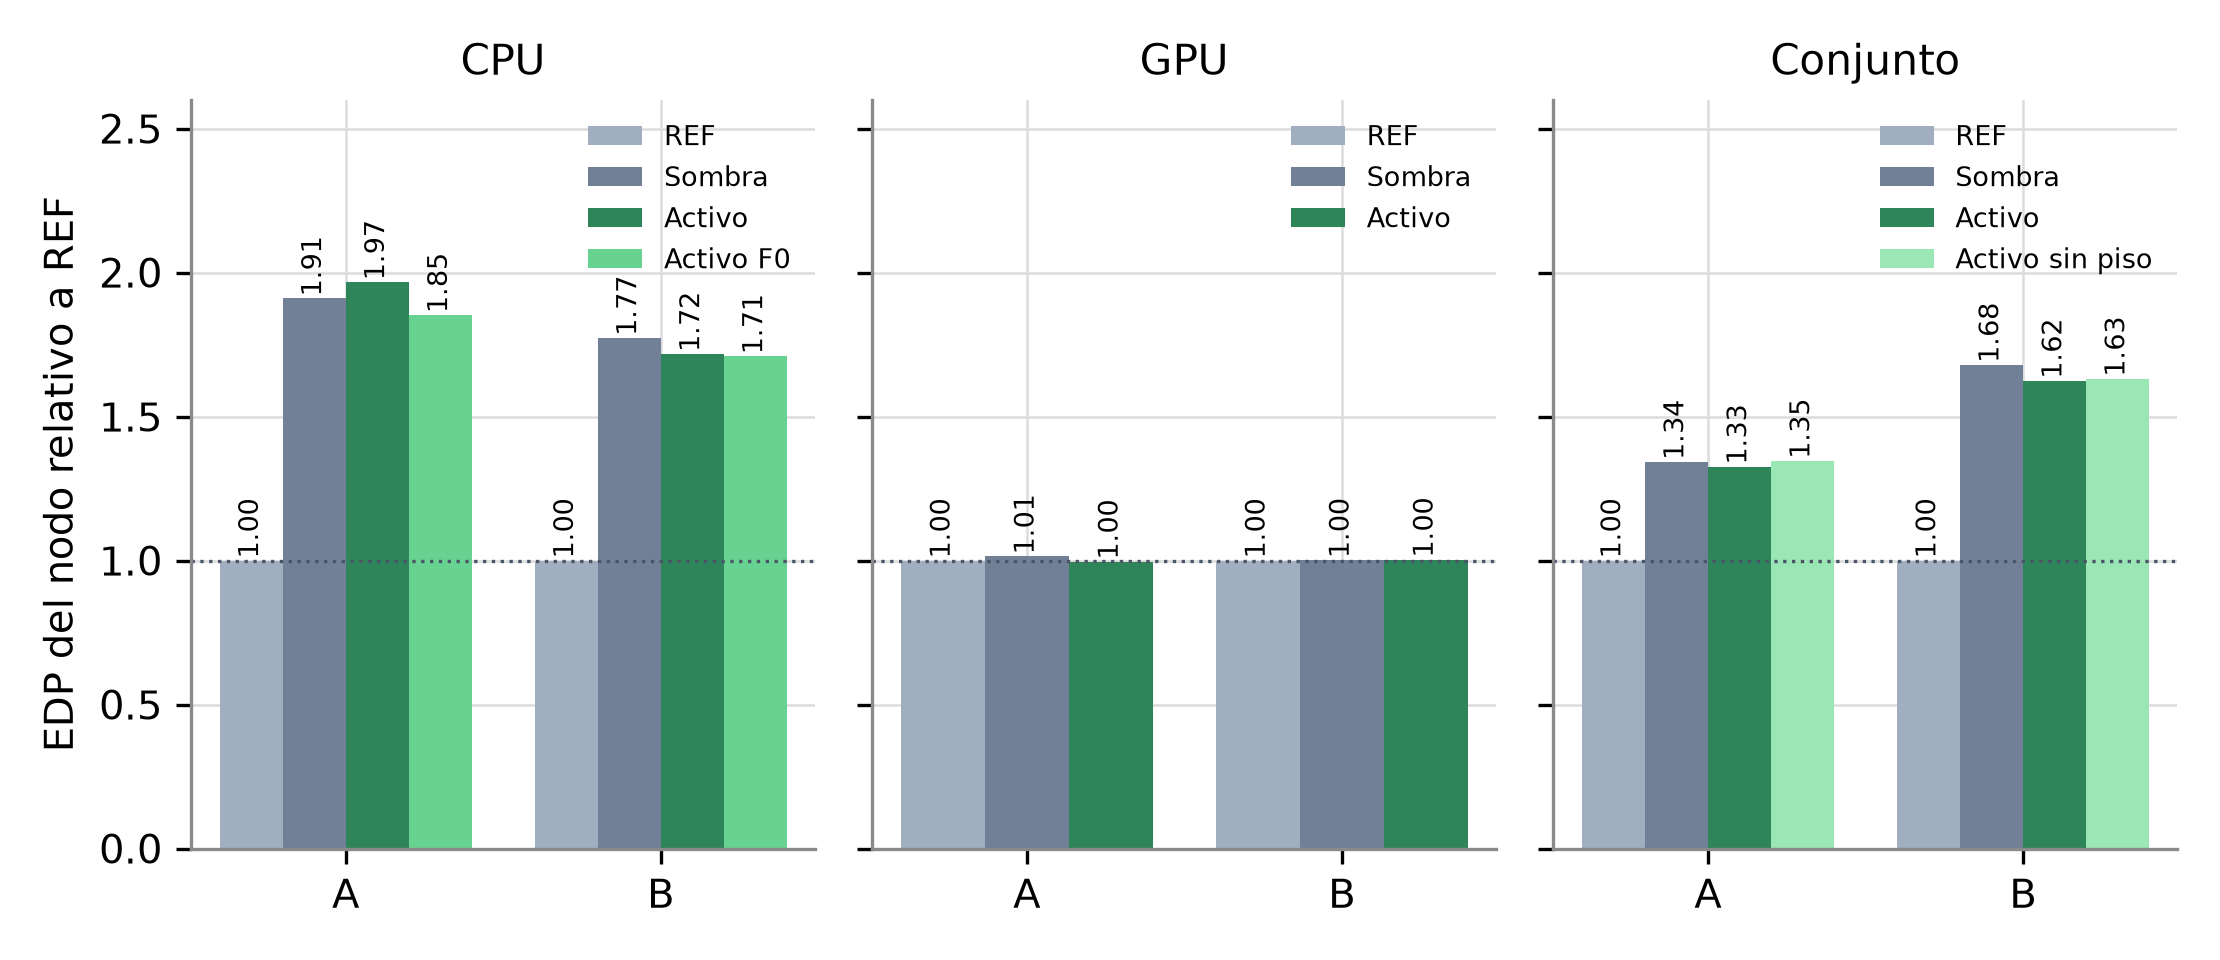
\includegraphics[width=\textwidth]{figuras/fig_fase4_edp_alcance_20260924.png}
    \caption{EDP del nodo, $(E_{\mathrm{CPU}} + E_{\mathrm{GPU}})\,T$, relativo a REF, por alcance, aplicación (A: vistos, B: inéditos) y brazo, en la matriz inicial. La línea punteada marca la paridad con REF.}
    \label{fig:fase4-edp}
\end{figure}





\subsection{Costo del agente de CPU y configuración de la inferencia}
\label{sec:resultados-fase4-costo}

La Figura \ref{fig:fase4-costo} desglosa el costo del agente. El brazo sombra permite medir el costo de mantener el agente en funcionamiento sin el efecto de la frecuencia. La causa del exceso de CPU no es el ritmo de muestreo: pasar de 1 a 10~ms reduce unas diez veces el número de decisiones y el costo no cambia (Tabla \ref{tab:fase4-costo}). Depende de la configuración del motor de inferencia. Con el conjunto de hilos por defecto, el motor de inferencia crea un hilo por núcleo que espera de forma activa entre inferencias y compite con la aplicación, que está fijada a los núcleos 0 a 3. Un único hilo de inferencia sin espera activa elimina la diferencia de tiempo (1.00 frente a REF) y reduce el sobrecosto de energía de CPU de 66\% a 6\%, y sube la exactitud de clasificación a 0.991; una explicación plausible, no verificada, es que las ventanas de contadores salen menos perturbadas cuando el agente no compite con la aplicación. Fijar el proceso consumidor a un núcleo no tiene efecto por sí solo. El agente de CPU se define, por tanto, con un hilo de inferencia; el agente de GPU no presentó este costo.



El sobrecosto de energía de CPU que queda con un hilo de inferencia no depende del periodo de muestreo: con kernels vistos, el brazo sombra queda en 1.086, 1.058 y 1.066 veces la energía de CPU de REF con periodos de 1, 10 y 100~ms (tres repeticiones cada uno), con exactitud de 97.6, 99.4 y 98.4\%. Es un costo fijo de mantener el agente, del orden de 6\%. La comparación completa del brazo activo con el agente definido con un hilo de inferencia es el escenario C (sección \ref{sec:resultados-fase4-C}).

\begin{figure}[H]
    \centering
    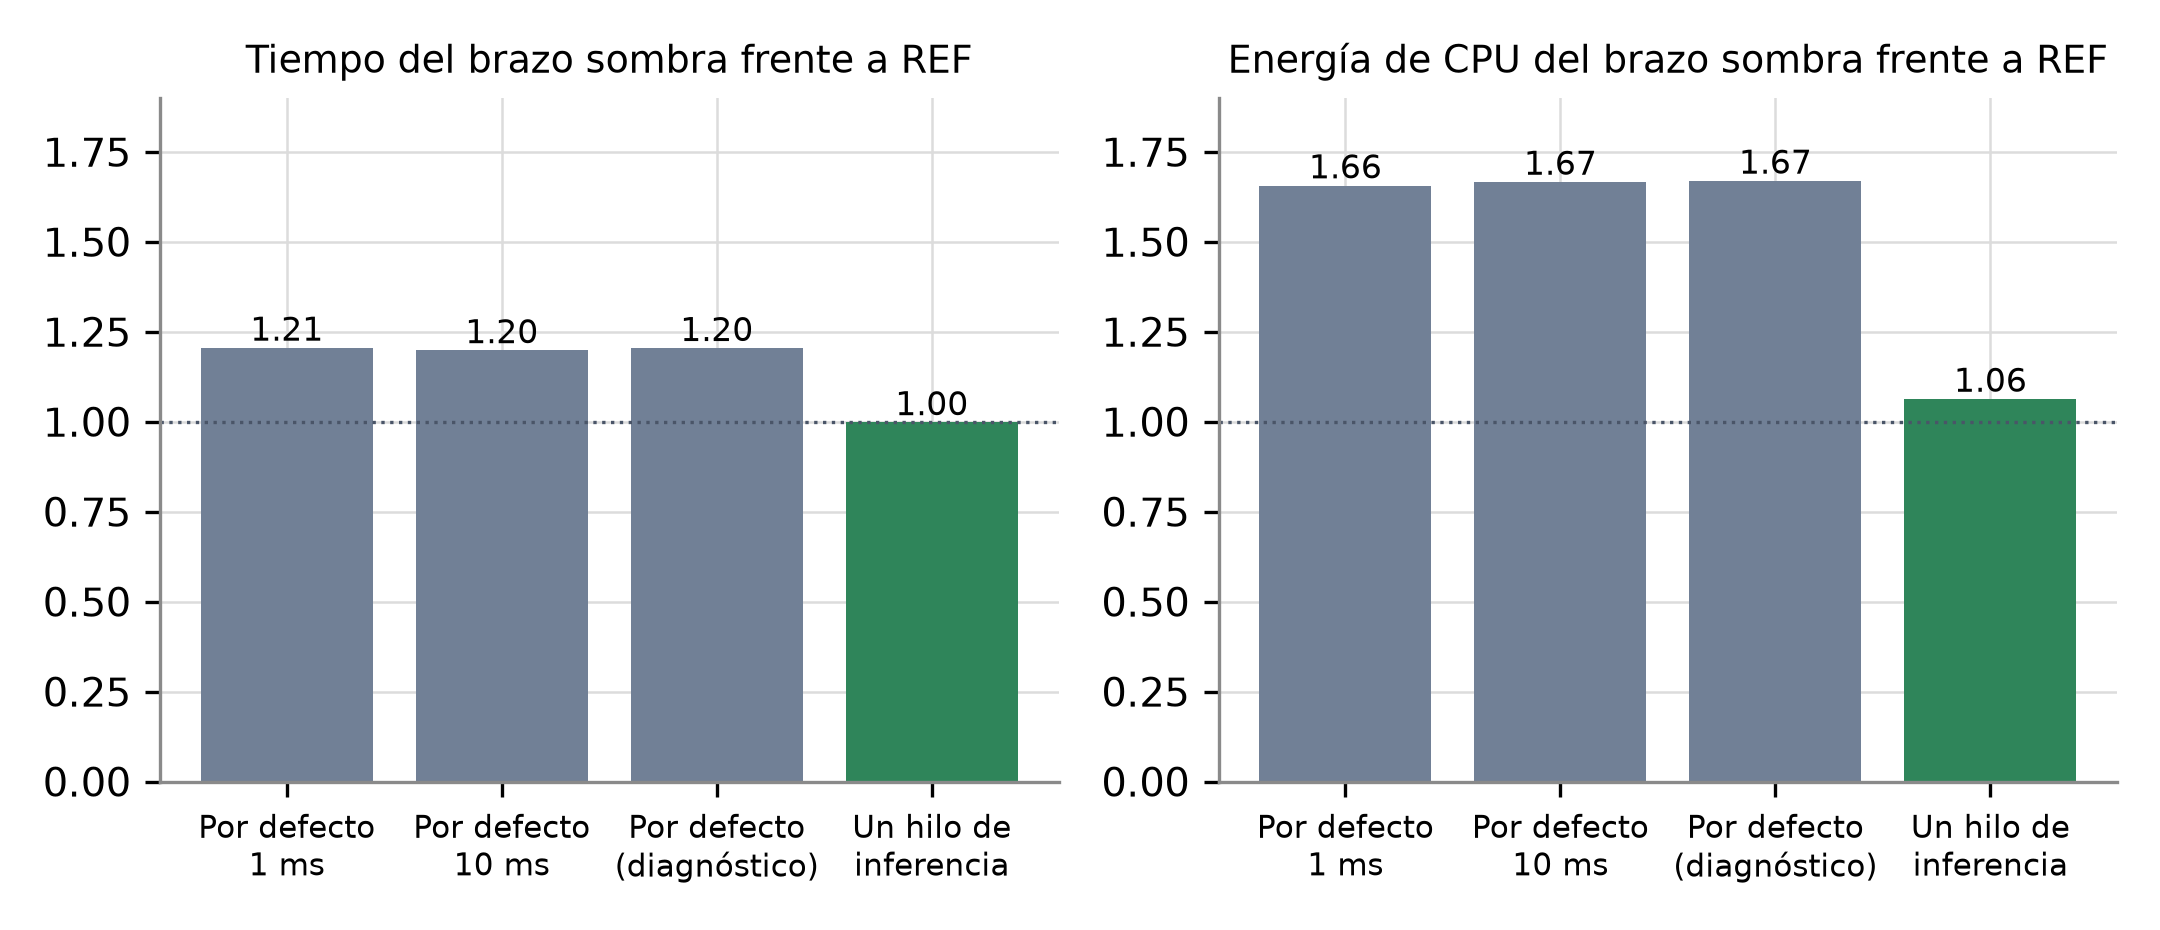
\includegraphics[width=0.94\textwidth]{figuras/fig_fase4_costo_agente_cpu_20260924.png}
    \caption{Costo del brazo sombra frente a REF en CPU con kernels vistos (A), por configuración de la inferencia y periodo de muestreo.}
    \label{fig:fase4-costo}
\end{figure}

\subsection{Potencial de la GPU}
\label{sec:resultados-fase4-gpu}

La ganancia máxima que la política de GPU puede aportar está acotada por la Fase 2: fijar el reloj en F1 (1260~MHz) durante fases \textit{memory\_bound} mejora el EDP en 8.9\% (IC95 3.0 a 13.3\%), y los niveles más bajos no mejoran o empeoran (Figura \ref{fig:fase4-gpu}, izquierda). El efecto sobre una aplicación completa se reduce por la fracción de su tiempo en memoria. Con 36\% (A) y 49\% (B) de fases \textit{memory\_bound}, la ganancia esperada del nodo es de 3.2\% y 4.3\%. La ganancia medida fue de 0.4\% en A y de $-0.3\%$ en B (Figura \ref{fig:fase4-gpu}, derecha), indistinguibles de cero con tres repeticiones.

\begin{figure}[H]
    \centering
    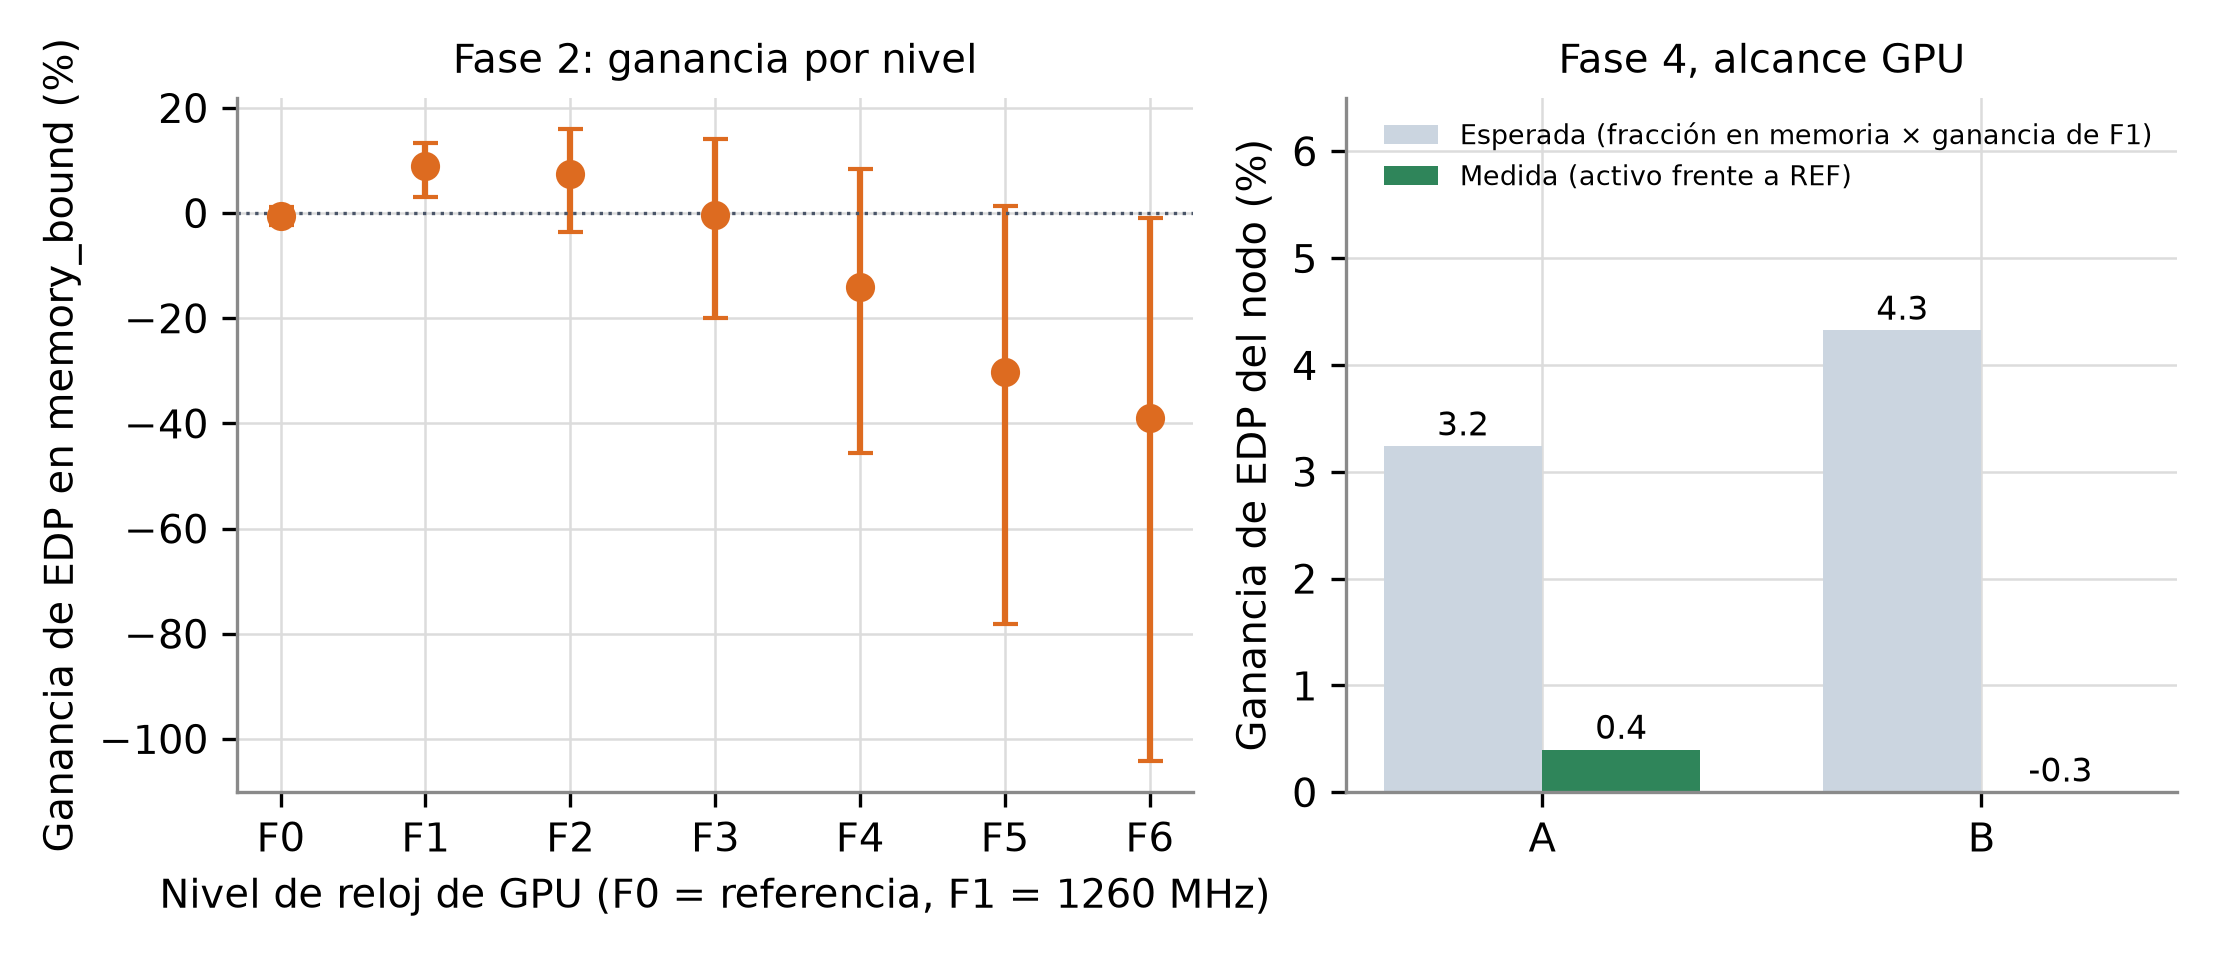
\includegraphics[width=\textwidth]{figuras/fig_fase4_gpu_potencial_20260924.png}
    \caption{Izquierda: ganancia de EDP por nivel de reloj de GPU en fases \textit{memory\_bound} (Fase 2, IC95 sobre familias). Derecha: ganancia esperada (fracción de tiempo en memoria por la ganancia de F1) frente a la medida con el agente activo en el alcance GPU.}
    \label{fig:fase4-gpu}
\end{figure}

En A, el agente clasificó las dos fases de \textit{triad} y aplicó F1 en ambas, y aun así la ganancia medida queda por debajo de la esperada: con tres repeticiones no puede separarse de cero y su causa no está aislada. En B, las fases de BabelStream, de 8~s, se resolvieron con una sola decisión cada una y en las celdas revisadas esa decisión fue una abstención, así que el reloj no se bajó. La ganancia posible de la GPU depende entonces de dos condiciones: que la aplicación pase una parte apreciable del tiempo en fases largas \textit{memory\_bound}, y que el agente no se abstenga en ellas. El escenario E de la sección \ref{sec:resultados-fase4-E} evalúa ambas.

\subsection{Escenario C: agente de CPU con un hilo de inferencia}
\label{sec:resultados-fase4-C}

Este escenario repite el alcance de CPU y el conjunto con el agente en su configuración final (un hilo de inferencia, sección \ref{sec:resultados-fase4-costo}), con tres repeticiones por brazo (Tabla \ref{tab:fase4-C} y Figura \ref{fig:fase4-C}). El costo de mantener el agente pasó a ser pequeño: el brazo sombra queda entre 1.036 y 1.094 del EDP de REF, con un exceso de tiempo de 0.4 a 1.4\% y un exceso de energía de CPU de 5 a 9\%. El brazo activo queda entre 1.05 y 1.16 y no mejora sobre sombra: el cociente activo/sombra es 1.06, 1.00, 1.02 y 1.01. En CPU con kernels vistos, bajar a F1 en memoria (1.161) es peor que mantener F0 (1.096). Quitar el piso de coordinación en el alcance conjunto empeora el EDP entre 0.8 y 1.3 puntos, de modo que el piso tiene un efecto pequeño pero favorable. La clasificación mantiene su exactitud con el agente corregido: 97.6\% en A y 99.9\% en B en CPU, sin errores en las decisiones de GPU (Tabla \ref{tab:fase4-clasificacion-CE}).

\begin{figure}[H]
    \centering
    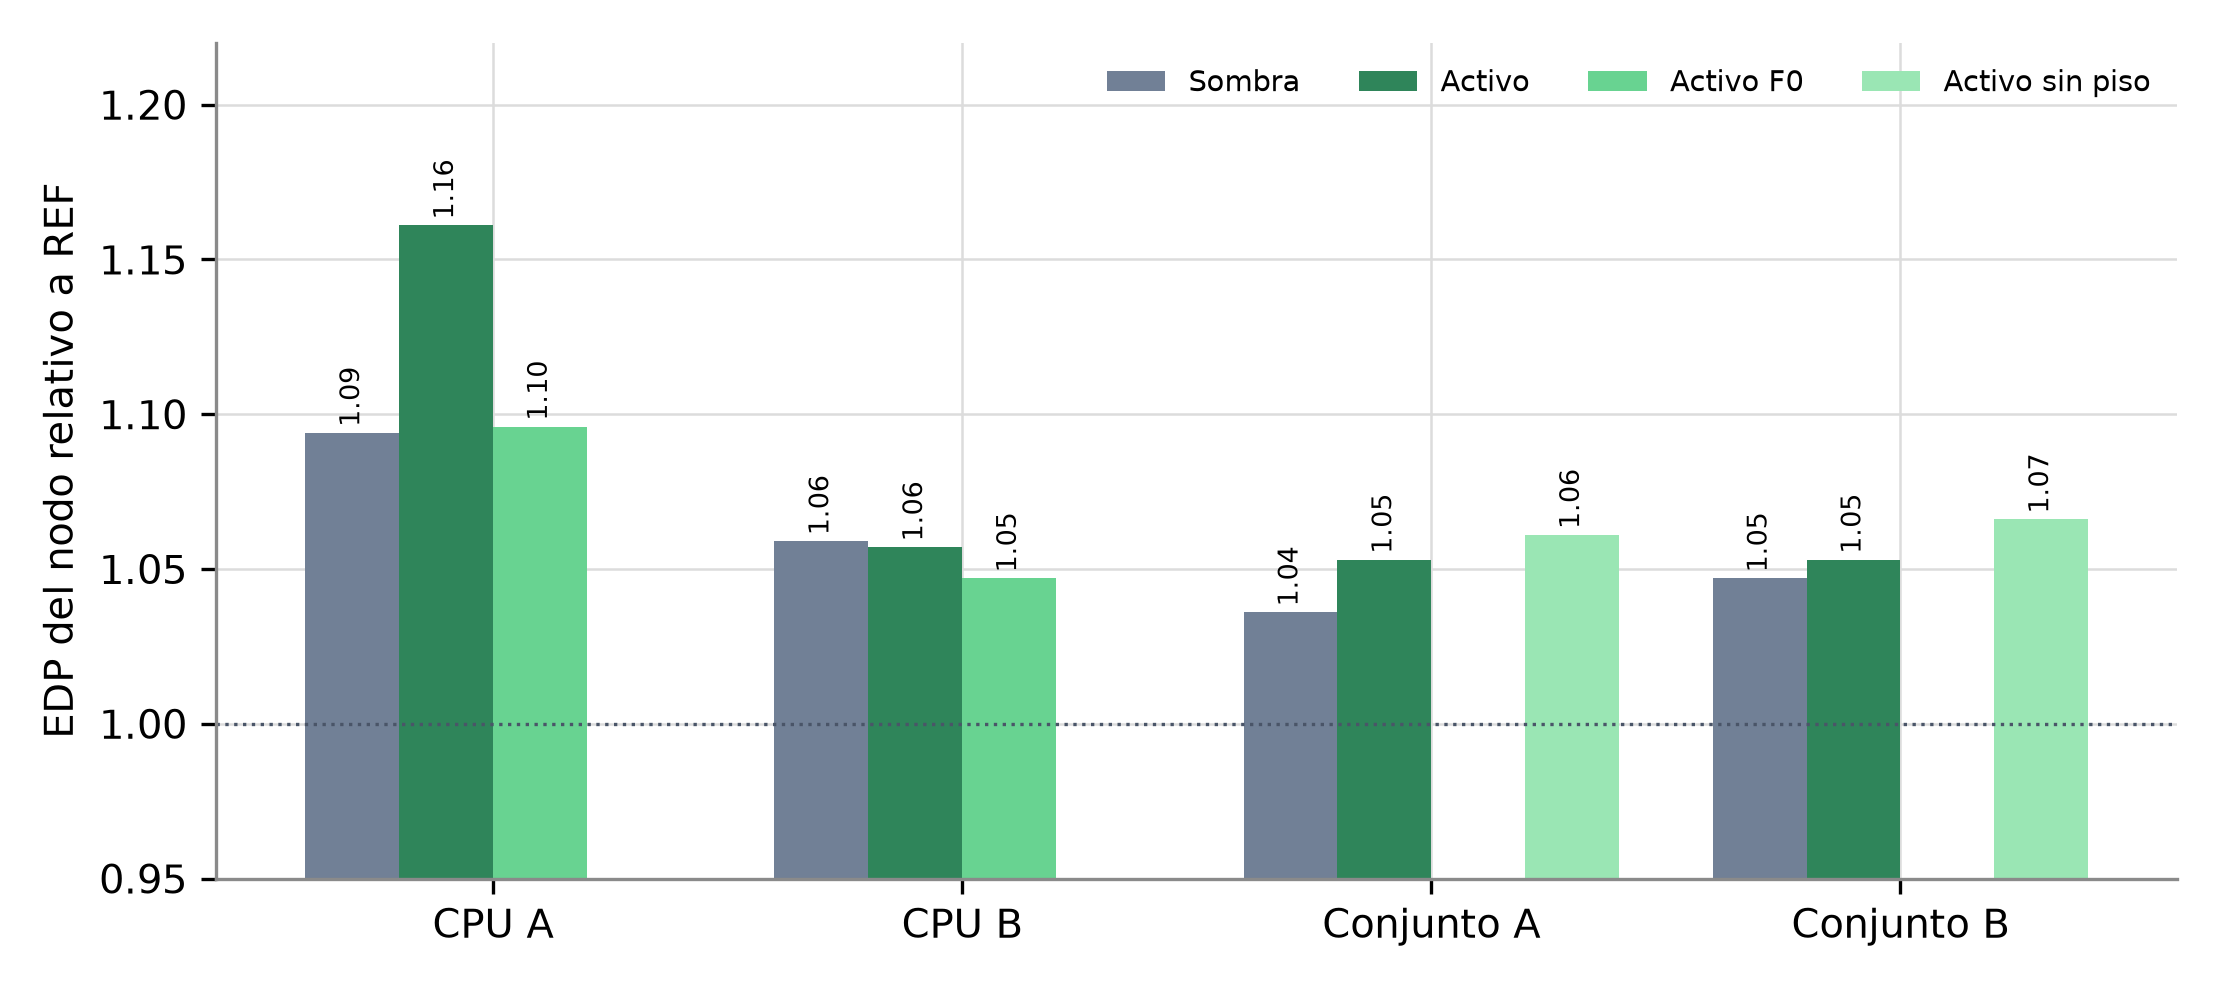
\includegraphics[width=\textwidth]{figuras/fig_fase4_C_edp_20260924.png}
    \caption{EDP del nodo relativo a REF en el escenario C, por alcance, aplicación y brazo. La línea punteada marca la paridad con REF.}
    \label{fig:fase4-C}
\end{figure}



\subsection{Referencia sin turbo}
\label{sec:resultados-fase4-noturbo}

REF sin turbo produjo razones medianas de EDP de 0.988 a 1.006 frente a REF en las seis combinaciones compuestas medidas (Tabla \ref{tab:fase4-noturbo}). En estas cargas el turbo no elevó el reloj sobre el límite de 3.2~GHz; por ello, las conclusiones CPU no dependen de esa línea base. La comparación no se extiende a LAMMPS ni CloverLeaf, ni sustituye un brazo de GPU con F1 fijo.



\subsection{Escenario E: GPU dominada por fases de memoria}
\label{sec:resultados-fase4-E}

El escenario E mide la política de GPU en las condiciones en que la Fase 2 predice ganancia: aplicaciones cuyo tiempo se reparte sobre todo en fases \textit{memory\_bound} largas. Es un escenario de aplicabilidad y no representa cualquier carga. Se definió antes de ejecutarse con un criterio de selección explícito: familias \textit{memory\_bound} cuya ganancia de EDP con F1 en la Fase 2 fue de al menos 10\%, más una variante con familias no vistas en el entrenamiento. La duración de las fases sale de una medición previa: el agente de GPU decide una vez por fase y la primera decisión llega entre 13 y 16~s después de su inicio, de modo que fases de 18~s pasan solo la mitad de su tiempo en F1 y fases de 45 a 60~s pasan más del 70\%.

La Tabla \ref{tab:fase4-E-composicion} resume las dos aplicaciones declaradas antes de medir. En B, \textit{myocyte} recibe una etiqueta de memoria por kernel pero casi no ocupa la GPU; solo el 42\% del ciclo corresponde a memoria con actividad GPU. Esta diferencia entre etiqueta y oportunidad de actuación condiciona la interpretación del resultado.

\begin{table}[H]
\centering
\caption{Composición del escenario E. Duraciones aproximadas por fase medidas antes de la matriz.}
\label{tab:fase4-E-composicion}
\small
\setlength{\tabcolsep}{3pt}
\begin{tabular}{@{}p{2.0cm}p{7.2cm}p{3.8cm}@{}}
\toprule
\textbf{Aplicación} & \textbf{Fases} & \textbf{Tiempo etiquetado memoria} \\
\midrule
A (vistas) & Stencil (58--60~s), SpMV (46~s), AXPY (47--48~s); DGEMM cómputo (31~s) & 84\% del ciclo \\
B (inéditas) & BabelStream (36~s), Myocyte (40--41~s); LavaMD cómputo (9~s) & 89\% etiquetado; 42\% con actividad GPU de memoria \\
\bottomrule
\end{tabular}
\end{table}

\paragraph{Medición exploratoria en familias vistas (A).} La medición exploratoria ejecutó tres repeticiones con REF, sombra y agente activo. El agente activo redujo la energía de GPU en 7.1\% (0.929 de REF), mantuvo la duración (1.000) y redujo el EDP del nodo a 0.975 y el EDP de GPU sola a 0.928 (Tabla \ref{tab:fase4-E} y Figura \ref{fig:fase4-E}). Sombra quedó en 0.995 del EDP de REF, lo que localiza la mayor parte del ahorro en la actuación F1. El agente clasificó y aplicó F1 en las fases de memoria previstas. La confirmación prospectiva de cinco bloques se reporta por separado a continuación.

El ahorro del nodo es modesto porque la CPU consume el 64\% de la energía en esta aplicación y no se modifica. Con el agente de CPU en observación, el EDP del nodo vuelve a 1.003, porque su costo (2.9\% más de energía de CPU y 1.0\% más de tiempo) iguala el ahorro de GPU. La configuración que mejora es, por tanto, la de un agente de GPU sin agente de CPU, coherente con la política de CPU de no actuar.

\paragraph{Confirmación prospectiva de E-A.} La mejora frente a REF se repitió en un confirmatorio declarado antes de medir, con cinco bloques aleatorizados y cinco repeticiones válidas por brazo. El brazo activo redujo la energía de GPU a 0.9282 de REF, mantuvo la duración en 0.9990 y dejó el EDP del nodo en 0.9716, equivalente a una reducción de 2.84\%. El brazo sombra quedó en 0.9935, por lo que el efecto no se explica por el costo de observación. Las cinco diferencias activo--REF fueron favorables; con bloques como unidad, la prueba exacta bilateral tiene $p=0.0625$, el mínimo posible para este diseño. El brazo F1 fijo no produjo celdas válidas, porque el reloj observado bajo carga quedó fuera del intervalo de 1230--1290~MHz exigido por el protocolo. Por ello, el confirmatorio reproduce la mejora frente a REF, pero no permite establecer la ventaja del cambio por fase frente a mantener F1 durante toda la aplicación.

\paragraph{Premedición de F1 fijo.} Antes del confirmatorio se ejecutó la medición diagnóstica F, con cinco repeticiones de REF y de una solicitud de F1 en DGEMM de CUTLASS, Conv2D y LavaMD. No se integra con E-A ni se usa para estimar el efecto del agente. En Conv2D y LavaMD, el EDP de GPU sola fue 0.894 y 0.960 de REF, respectivamente, pero el EDP del nodo fue 1.017 y 1.024 por el aumento del tiempo. En DGEMM, el reloj observado con F1 solicitado fue de 1140 a 1155~MHz, indistinguible de REF, por lo que esa comparación no valida una actuación a 1260~MHz. Este antecedente motivó el criterio de reloj bajo carga que después invalidó el brazo fijo del confirmatorio E-A.

\paragraph{Familias inéditas (B).} La mediana quedó cerca de paridad (EDP de nodo 1.014 y energía GPU 1.003 de REF). BabelStream recibió una decisión de memoria en una de tres repeticiones y allí ahorró 12\% de energía GPU y 5\% de EDP del nodo; en las otras dos se abstuvo. \textit{Myocyte} no superó sostenidamente el umbral de actividad GPU y no recibió decisión. Una demora aislada de esa fase ocurrió sin cambio de reloj atribuible al agente. El límite observado es la cobertura de decisión sobre familias inéditas, no un empeoramiento sistemático por F1.

\begin{figure}[H]
    \centering
    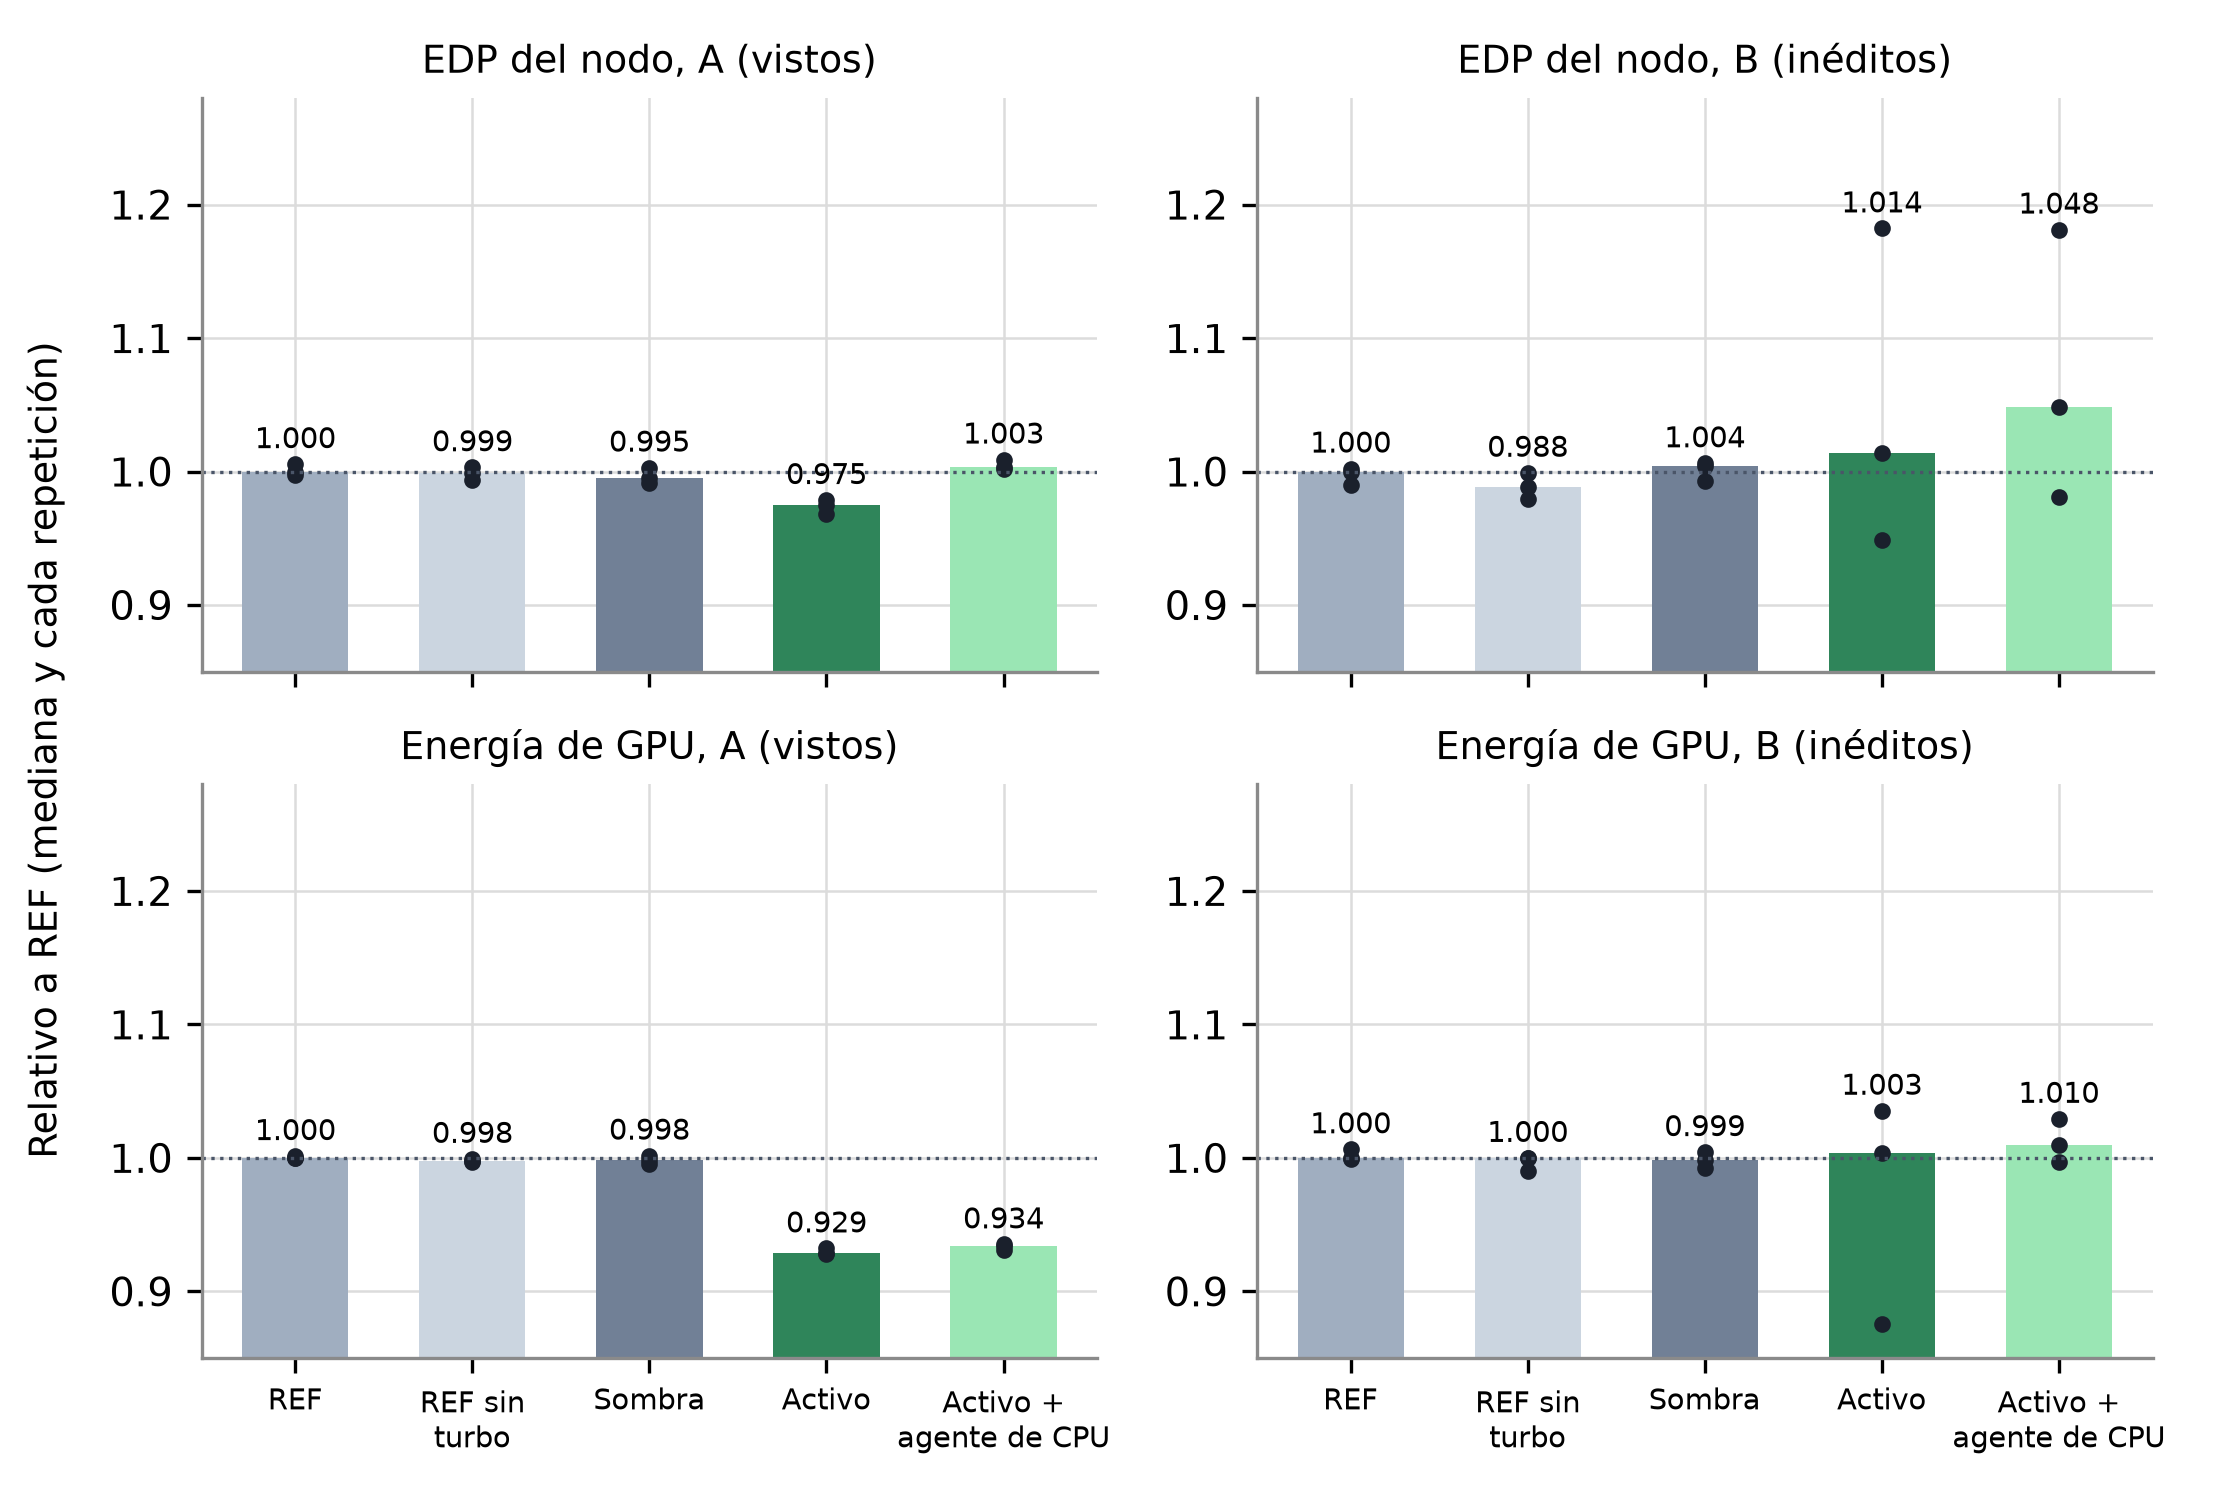
\includegraphics[width=\textwidth]{figuras/fig_fase4_E_20260924.png}
    \caption{Escenario E. EDP del nodo (arriba) y energía de GPU (abajo) relativos a REF, con la mediana (barra) y cada repetición (punto), para las aplicaciones de familias vistas (A) e inéditas (B).}
    \label{fig:fase4-E}
\end{figure}





\subsection{Escenario D: LAMMPS como aplicación de terceros}
\label{sec:resultados-fase4-D}

El escenario D evalúa LAMMPS 2023 con el paquete GPU del clúster, sin imponer fronteras de fase al programa. Se ejecutaron tres bloques de las entradas \texttt{chain}, \texttt{eam}, \texttt{lj} y \texttt{rhodo}, con REF, sombra, agente de GPU activo y una variante que mantiene el agente de CPU en observación. Todas las 48 celdas terminaron con código de aplicación y de daemon válido, y restauraron el estado de frecuencia. La Figura \ref{fig:fase4-D} y la Tabla \ref{tab:fase4-D} muestran que el brazo activo de GPU queda entre 0.998 y 1.008 de REF en EDP, según la entrada. No se observa una mejora persistente y la variante con el agente de CPU en observación incrementa el EDP entre 3.0 y 4.3\%. En \texttt{chain} y \texttt{rhodo} el agente no emitió decisiones y en \texttt{lj} y \texttt{eam} solo emitió \textit{compute\_bound}, por lo que no aplicó F1. Este resultado extiende la evaluación a una aplicación externa, pero no mide el efecto de la política GPU sobre una fase actuada.

\begin{figure}[H]
    \centering
    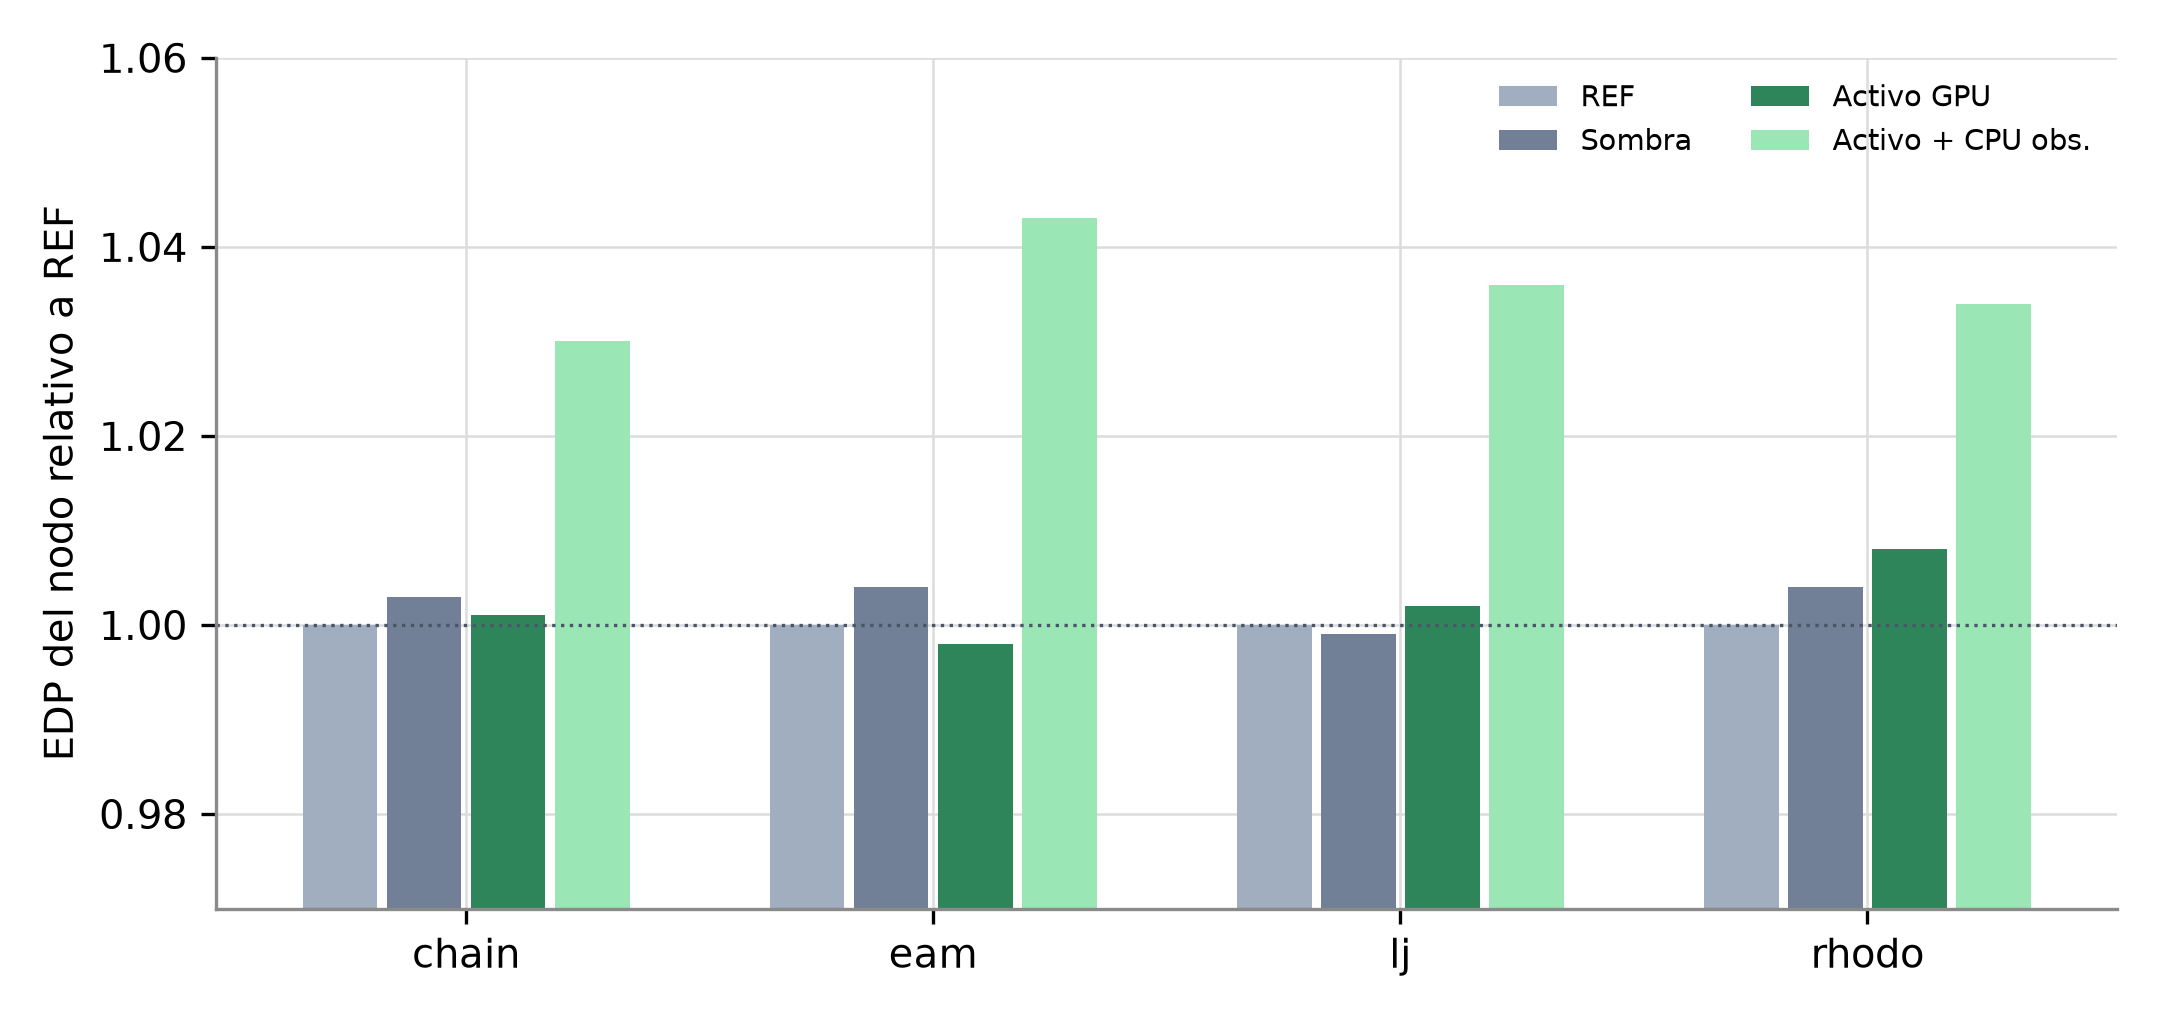
\includegraphics[width=0.88\textwidth]{figuras/fig_fase4_D_20260924.png}
    \caption{EDP mediano de LAMMPS por entrada y brazo, relativo a REF. Fuente: elaboración propia.}
    \label{fig:fase4-D}
\end{figure}



\subsection{CloverLeaf CUDA Fortran como aplicación continua}
\label{sec:resultados-fase4-cloverleaf}

CloverLeaf CUDA Fortran se evaluó como una aplicación continua de dinámica de fluidos, sin fronteras de fase impuestas al programa. El confirmatorio ejecutó cinco bloques aleatorizados con REF, sombra y activo. Las quince corridas terminaron con código de aplicación válido, restauración correcta del reloj y solución numérica reproducible; la energía cinética final fue idéntica dentro de la tolerancia relativa de $10^{-8}$. En cada corrida activa el agente emitió una decisión \textit{memory\_bound} con confianza 1.00 tras aproximadamente 3~s y solicitó 1260~MHz. Tras esa decisión, las 433 o 434 muestras NVML bajo carga de cada bloque permanecieron en 1260~MHz. CloverLeaf no aporta una etiqueta Roofline independiente por fase, de modo que este experimento verifica la actuación y su efecto energético, pero no puntúa la exactitud de esa decisión. La Tabla \ref{tab:fase4-cloverleaf} resume las medianas y las razones frente a REF.

El brazo activo mantuvo la duración en 1.0015 de REF, redujo la energía de GPU a 0.9393 y dejó el EDP del nodo en 0.9625, una reducción de 3.75\%. El brazo sombra quedó en 0.9958 de EDP, por lo que no se observa un costo apreciable de mantener el agente sin actuar. Las cinco diferencias de EDP activo--REF fueron favorables; la prueba exacta bilateral por bloques da $p=0.0625$, que no alcanza el umbral de 0.05. La Figura \ref{fig:fase4-cloverleaf-edp} muestra las cinco observaciones emparejadas por bloque y la Figura \ref{fig:fase4-cloverleaf-energia} descompone el resultado entre CPU y GPU. En este caso, la actuación reduce la energía del dispositivo sin modificar de forma apreciable el tiempo de ejecución.

\begin{figure}[H]
    \centering
    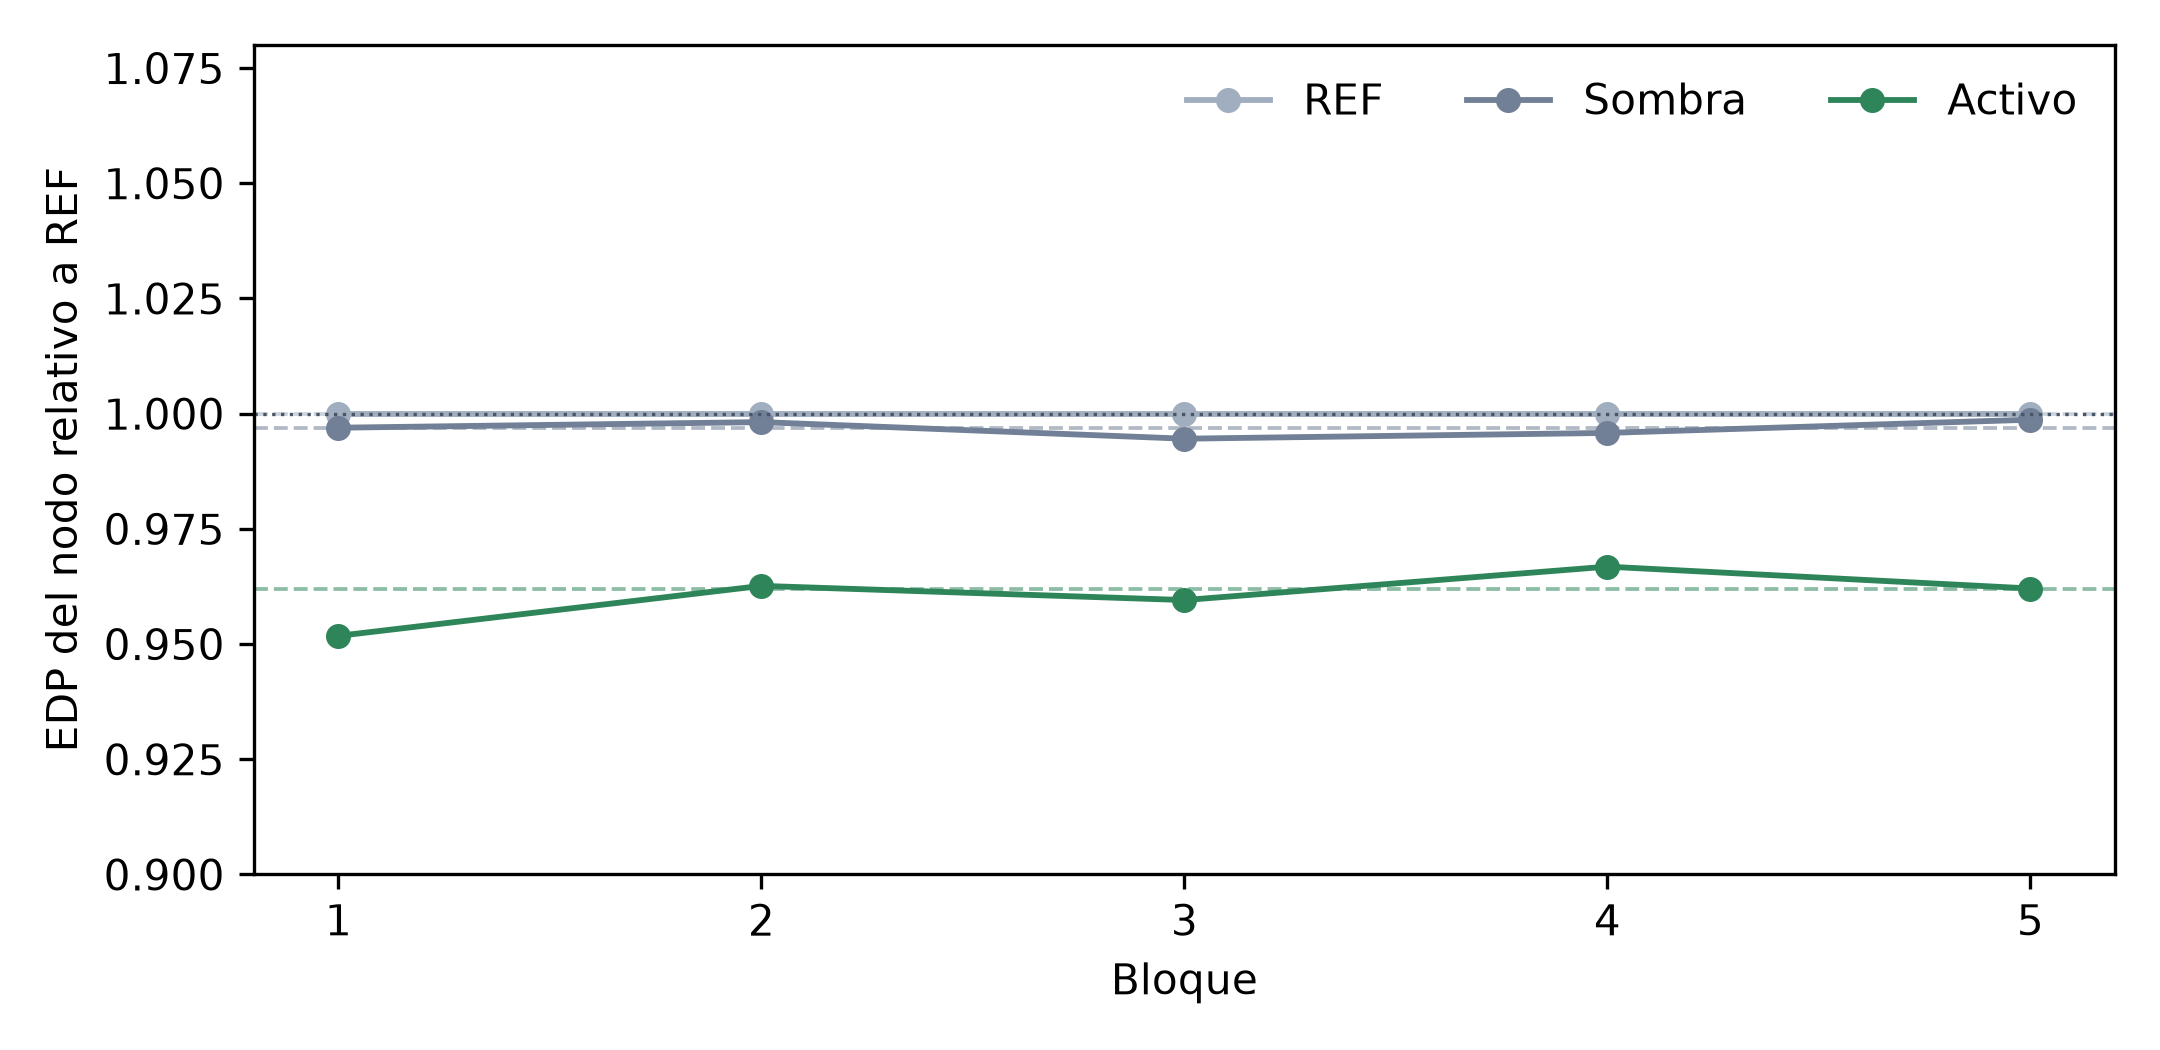
\includegraphics[width=0.90\textwidth]{figuras/fig_fase4_cloverleaf_edp_20260924.png}
    \caption[EDP de CloverLeaf por bloque y brazo]{EDP del nodo de CloverLeaf relativo a REF en cada bloque. Las líneas discontinuas indican la mediana de cada brazo y la línea punteada marca la paridad con REF. Fuente: elaboración propia a partir de cinco bloques del nodo \texttt{paccaA100}.}
    \label{fig:fase4-cloverleaf-edp}
\end{figure}

\begin{figure}[H]
    \centering
    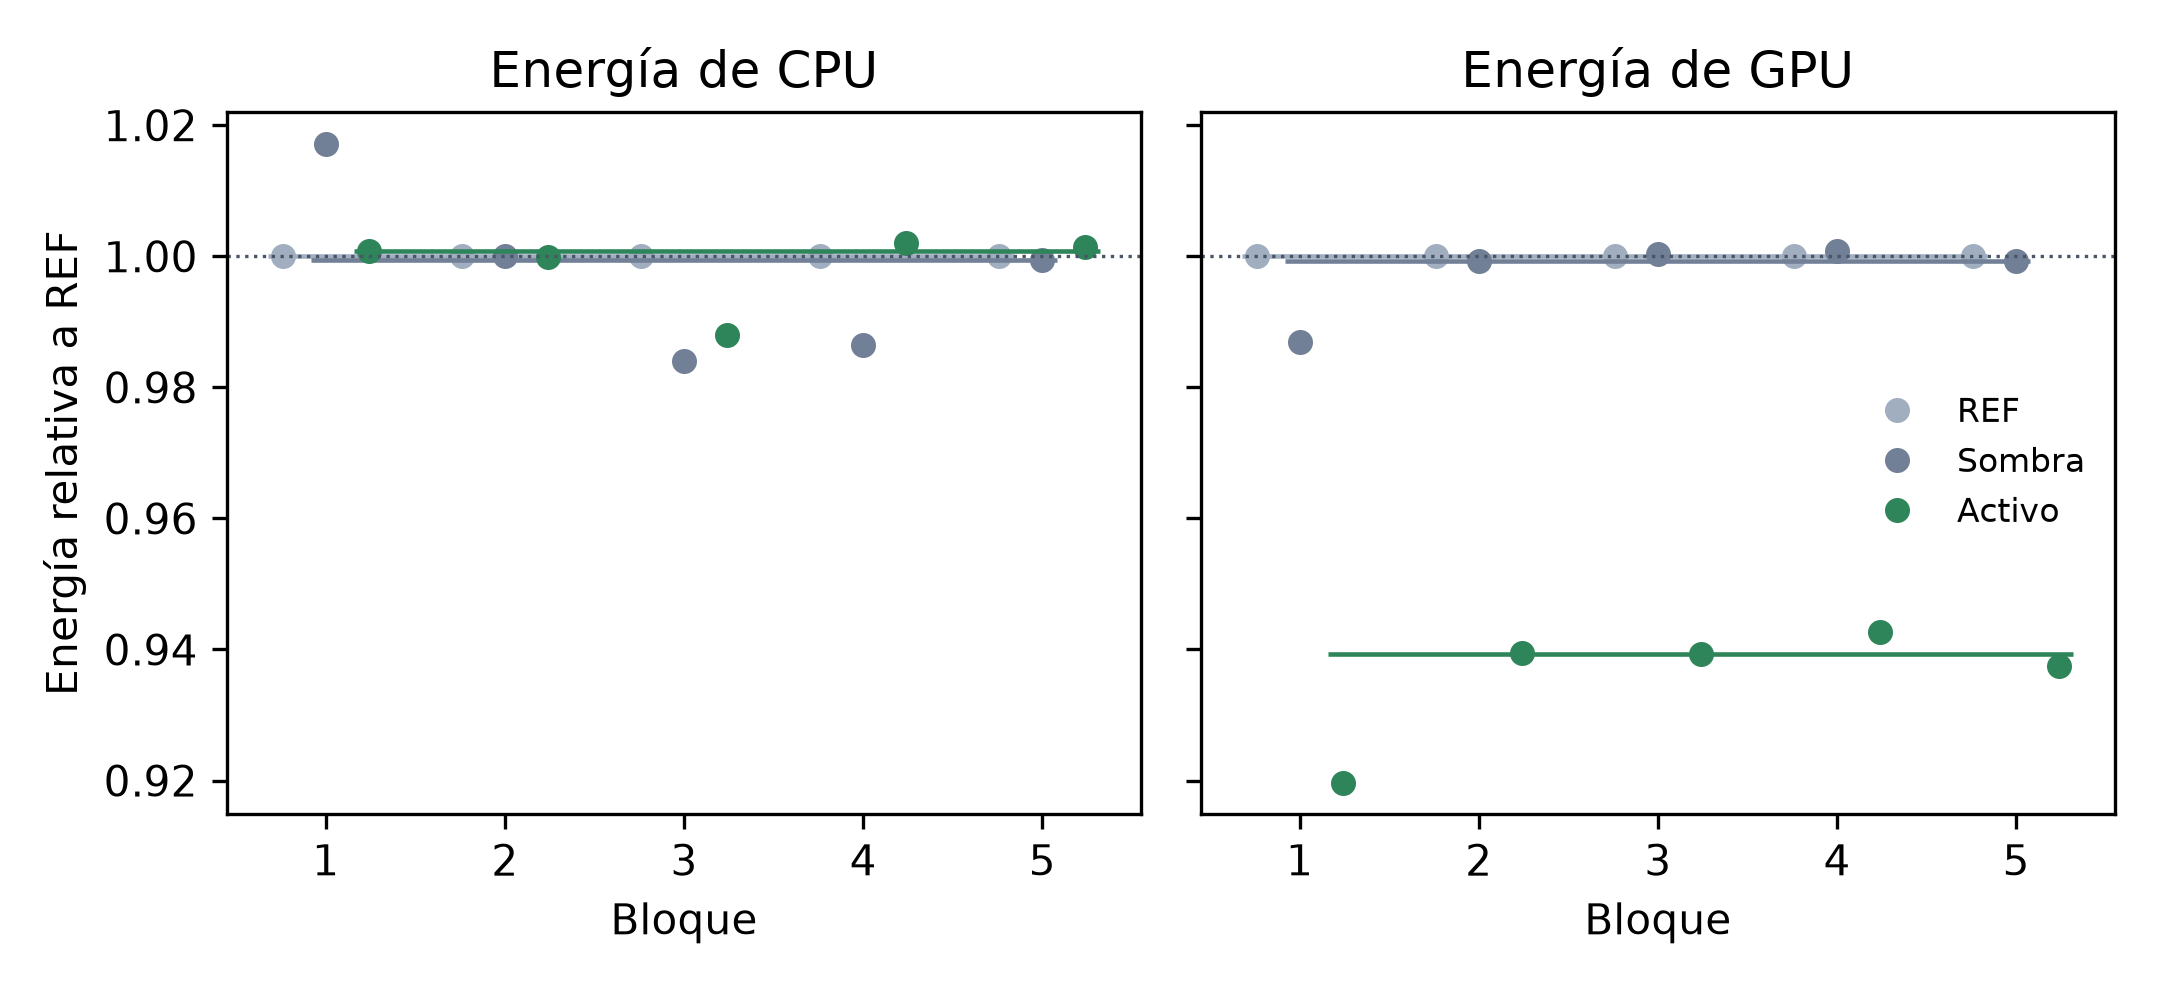
\includegraphics[width=0.90\textwidth]{figuras/fig_fase4_cloverleaf_energia_20260924.png}
    \caption[Descomposición de energía de CloverLeaf]{Energía de CPU y GPU de CloverLeaf relativa a REF en los cinco bloques. Los puntos representan bloques individuales y las líneas horizontales, las medianas por brazo. Fuente: elaboración propia.}
    \label{fig:fase4-cloverleaf-energia}
\end{figure}





\begin{table}[H]
\centering
\caption{Resultados del confirmatorio de CloverLeaf CUDA Fortran. Duración y energías son medianas de cinco bloques; las razones se calculan frente a REF.}
\label{tab:fase4-cloverleaf}
\small
\begin{adjustbox}{max width=\textwidth}
\begin{tabular}{@{}lrrrrrr@{}}
\toprule
\textbf{Brazo} & \textbf{$n$} & \textbf{$T$ (s)} & \textbf{$E_{\mathrm{CPU}}$ (J)} & \textbf{$E_{\mathrm{GPU}}$ (J)} & \textbf{EDP/REF} & \textbf{$E_{\mathrm{GPU}}$/REF} \\
\midrule
REF & 5 & 112.032 & 16939.3 & 27729.5 & 1.0000 & 1.0000 \\
Sombra & 5 & 111.975 & 16923.4 & 27733.6 & 0.9958 & 1.0001 \\
Activo & 5 & 112.201 & 16957.7 & 26044.9 & 0.9625 & 0.9393 \\
\bottomrule
\end{tabular}

\end{adjustbox}
\end{table}

\subsection{Balance de la Fase 4}
\label{sec:resultados-fase4-balance}

La Tabla \ref{tab:fase4-balance} reúne la respuesta a cada pregunta de la Fase 4 y distingue los resultados favorables, neutros y no demostrados.

\begin{table}[H]
\centering
\caption{Balance de la Fase 4. El desglose por pregunta se conserva en la Tabla \ref{tab:fase4-balance-detalle} del Anexo \ref{anexo:resultados-complementarios}.}
\label{tab:fase4-balance}
\small
\begin{tabular}{@{}p{3.5cm}p{9.8cm}@{}}
\toprule
\textbf{Pregunta} & \textbf{Resultado} \\
\midrule
Clasificación & Alta en aplicaciones con verdad conocida; la GPU se abstiene con frecuencia ante familias inéditas \\
Costo de observación & GPU sin costo medible; CPU con un hilo añade 5 a 9\% de energía \\
Actuación CPU & Sin mejora de EDP frente a REF ni frente a sombra \\
Actuación GPU & E-A: $-2.84\%$ de EDP del nodo; CloverLeaf: $-3.75\%$; LAMMPS: paridad \\
F1 fijo & La comparación directa quedó inválida por reloj no sostenido bajo carga \\
\bottomrule
\end{tabular}
\end{table}

\chapter{Discusión}

Los resultados sostienen dos tipos de contribución. La contribución metodológica corresponde a la construcción y verificación del instrumento antes de utilizar sus mediciones para entrenar. La contribución empírica corresponde al comportamiento real de la plataforma y a la capacidad de transferencia de los clasificadores CPU y GPU entre familias algorítmicas.

Buena parte de la literatura revisada en el estado del arte (los métodos de selección de frecuencia óptima de Ali et al. \cite{Ali2023} y de clasificación consciente de DVFS de Guerreiro et al. \cite{Guerreiro2019}, o el marco de control por refuerzo de Wang et al. \cite{Wang2024}) asume, de forma razonable dado su alcance, que la escritura de frecuencia sobre el hardware subyacente funciona como el fabricante la documenta, y concentra su aporte en la capa de decisión: qué frecuencia elegir, o cómo aprenderla. Los resultados de este trabajo muestran que esa suposición debe verificarse empíricamente bajo carga real y no darse por sentada en ningún mecanismo del instrumento: en GPU, el bloqueo de reloj sostuvo dos objetivos distintos durante cientos de lecturas activas bajo carga; en CPU, la actuación se confirma correctamente solo cuando se restringen tanto los procesadores lógicos delegados como sus hermanos de \textit{SMT} (sección \ref{sec:resultados-cpu-dvfs}), un resultado que hubiera pasado por una lectura de límites exitosa sin serlo si solo se hubiera verificado la primera condición. La misma disciplina de no asumir una capacidad de hardware sin contrastarla rige el presupuesto de nueve contadores físicos simultáneos y no diez, ajustado por la reserva que hace el vigilante NMI del sistema operativo (sección \ref{sec:resultados-interferencia-uncore}), y la validación cruzada de los techos Roofline contra Intel Advisor, con una coincidencia de 12 a 15\% pese a partir de mecanismos de medición independientes (sección \ref{sec:resultados-ppico}). Generalizar esta disciplina de verificación directa, incluida una prueba de humo a escala reducida antes de cualquier campaña de producción, es un aporte metodológico de esta fase tan relevante como los datos concretos que produjo.

El resultado CPU confirma que la abundancia de intervalos no equivale a disponer de muchas unidades independientes de generalización. Los 1.31 millones de intervalos elegibles proceden de 30 familias algorítmicas y más de la mitad de ellas es homogénea respecto de la clase Roofline. La magnitud de esa distinción se pudo cuantificar con el mismo modelo y los mismos datos: repartir intervalos al azar produce 0.874 de exactitud balanceada, dejar fuera un kernel completo 0.733 y dejar fuera una familia completa 0.728 (sección \ref{sec:resultados-cpu-protocolo}). La primera cifra no mide clasificación de régimen sino reconocimiento de la carga, y es la que obtendría un protocolo que no separase por familia. Esta comparación es, en sí misma, un argumento metodológico a favor de reportar la validación por familia aun cuando produzca cifras notablemente menores.

El resultado también acota qué palancas quedan disponibles. El algoritmo de aprendizaje, el tamaño del vector de entrada y los hiperparámetros resultaron indiferentes dentro del intervalo de confianza, y un clasificador de vecinos más cercanos sin ajuste alcanza 0.684 con el mismo protocolo. La literatura revisada concentra su aporte en esa capa de decisión, de modo que conviene precisar el alcance del hallazgo: no contradice esos métodos, pero muestra que, en este catálogo y con estas señales, la frontera entre regímenes no se mueve al cambiar de modelo. Lo que sí mueve el resultado es la diversidad algorítmica del catálogo, con una pendiente estimada de 0.037 por duplicación del número de familias. Esa relación convierte la construcción del catálogo, y no la selección del modelo, en la actividad determinante del desempeño alcanzable.

La política selectiva ofrece una respuesta operativa acotada a esa incertidumbre, aunque su ganancia debe dimensionarse con cuidado. Con el umbral congelado en 0.85 el modelo decide sobre el 72.2\% de los intervalos y su exactitud balanceada por celda pasa de 0.728 a 0.738, una ganancia modesta por celda que se ve con más fuerza en las métricas agrupadas (la F1 macro pasa de 0.760 a 0.842). Abstenerse al azar en la misma proporción no cambia el resultado, de modo que la mejora proviene efectivamente de que la confianza señala casos difíciles. Aun así, la diferencia entre la F1 macro agrupada, de 0.842, y el desempeño de las familias individuales muestra que el buen resultado se concentra en familias transferibles y no constituye una garantía uniforme para una carga inédita.

Un resultado independiente del clasificador, pero decisivo para el objetivo de eficiencia, es que la clase Roofline por sí sola no determina la frecuencia de menor producto energía--retardo. En el procesador estudiado, unos 85~W de potencia de paquete no dependen del reloj de los núcleos, de modo que reducirlo de 3.2 a 0.8~GHz ahorra solo 15\% de potencia mientras alarga el tiempo en proporción a $f^{-\alpha}$. La política resultante es no actuar en ambas clases, y ni siquiera un selector perfecto que eligiera el mejor nivel por kernel supera un techo medio de 2.2\% de ganancia, con 22 de los 47 kernels por debajo del efecto mínimo relevante. Dos pruebas externas selladas, con una regla congelada antes de medir sobre familias nuevas ajenas al entrenamiento, confirmaron que no hay un subconjunto de la clase memory-bound sobre el que sea seguro actuar con la evidencia disponible (sección \ref{sec:resultados-cpu-potencia-diseno}). La utilidad del clasificador reside, por tanto, en decidir cuándo abstenerse de actuar, más que en repartir frecuencias por clase.

La abstención tampoco corrige los errores de alta confianza, porque la confianza del modelo está mal calibrada fuera de su familia de entrenamiento: declara 0.890 en promedio frente a una exactitud observada de 0.764, con un error de calibración esperado de 0.126. Entre los intervalos con confianza mayor o igual a 0.9, \textit{npb\_ft} acierta el 32\% y \textit{npb\_mg} el 35\%. Por ello la probabilidad estimada por XGBoost no debe interpretarse como una probabilidad calibrada de acierto para cualquier familia inédita; su función actual es delimitar una región de operación bajo el conjunto disponible. Para la salida \textit{revisar}, la política conservadora evita convertir la incertidumbre en una actuación DVFS potencialmente perjudicial; darle a esa espera una acción concreta, mediante una medición física breve de la carga en ejecución, es un diseño que corresponde al agente de la Fase 3 y no a esta.

El hallazgo de precisión mixta en el catálogo de GPU (sección \ref{sec:resultados-precision-gpu}) es relevante más allá de este trabajo concreto. La práctica de derivar la precisión de caracterización de un kernel a partir de su tipo de dato declarado en el código fuente, en lugar de la precisión efectivamente ejercitada por el hardware durante su ejecución, es razonable como primera aproximación, pero este trabajo encontró que puede diferir de lo medido en más del 70\% del trabajo aritmético de un kernel, y que esa diferencia puede situarse exactamente en el margen que decide una clasificación Roofline. Ningún trabajo de los revisados en el estado del arte reporta explícitamente esta verificación para GPU, lo que sugiere que la práctica de asumir la precisión declarada, sin contrastarla, podría no ser inusual en caracterizaciones similares.

El resultado sobre precisión de \texttt{gpu\_dgemm\_n4096} (sección \ref{sec:resultados-precision-gpu}) matiza, sin contradecir, el hallazgo de Guerreiro et al. sobre la sensibilidad de las cargas GPGPU a la ruta de ejecución elegida por bibliotecas de terceros \cite{Guerreiro2019}: una ruta acelerada por hardware especializado invalida efectivamente un método de caracterización diseñado para instrucciones aritméticas convencionales, pero no invalida necesariamente la magnitud medida, siempre que exista una vía de verificación independiente, en este caso el conteo analítico del propio algoritmo, contra la cual contrastarla.

El reanálisis histórico de GPU delimita el alcance de la clasificación ligera. El conjunto A se utilizó para seleccionar el candidato y el conjunto B, una campaña histórica independiente de agosto, se mantuvo para la prueba externa. La mejora frente al diagnóstico inicial no surgió de seleccionar retrospectivamente el mejor resultado de B, sino de excluir la familia miniBUDE con control de reloj no verificable, agregar las lecturas NVML por corrida, comparar representaciones robustas y ponderar cada familia de forma equivalente durante el entrenamiento. Las razones físicas derivadas, los percentiles, las medias recortadas y la dinámica temporal se evaluaron como alternativas. La representación estática basada en medianas e IQR fue la única que conservó utilidad fuera de su campaña de origen. El F1 macro externo de 0.663 supera ampliamente la regla que siempre predice la clase mayoritaria, cuyo F1 macro fue 0.426, aunque ambas tienen la misma exactitud de 0.743. La igualdad en exactitud no es contradictoria. El modelo recupera 18 corridas \textit{compute\_bound} que la regla mayoritaria nunca reconoce y, a cambio, confunde 18 corridas \textit{memory\_bound}.

La abstención calibrada ofrece una alternativa operativa coherente con esta limitación. La política no altera la etiqueta ni elimina retrospectivamente casos cercanos al \textit{ridge}. Solo utiliza la confianza calculada a partir de las señales NVML disponibles en producción y devuelve \textit{revisar} cuando esa confianza no supera el umbral seleccionado dentro del entrenamiento. Al retirar de la decisión automática la región en que ambas clases presentan señales agregadas similares, la F1 macro de las decisiones cubiertas aumenta a 0.734. Esta cifra se informa junto con la cobertura de 93.9\%, por lo que no se interpreta como una mejora de cobertura total ni como sustituto de la evaluación externa en B. Esta salida permite diferir una proporción pequeña de decisiones inciertas a una caracterización posterior, en lugar de forzar una clase con evidencia insuficiente.

La separabilidad parcial de la Figura \ref{fig:gpu-separabilidad-nvml} explica esta conducta. En los datos históricos, la etiqueta procede de una intensidad operacional por kernel obtenida fuera de línea, mientras que la entrada reúne las señales de todo el intervalo de la corrida. NVML describe actividad, potencia y estado operativo de toda la GPU, pero no observa directamente instrucciones ejecutadas, tráfico de memoria, ocupación, causas de espera o la identidad del kernel activo. Cuando una ejecución tiene subfases con comportamiento distinto, el agregado conserva su efecto medio y pierde el orden y los límites de esas subfases. Por ello, una familia \textit{compute\_bound} puede ocupar una región cercana a una familia \textit{memory\_bound}. La visualización t-SNE no se interpreta como prueba de generalización, dado que su objetivo es preservar vecindarios locales y sus distancias globales no son métricas físicas. La silueta por clase de 0.092 y el F1 macro de 0.616 obtenido por vecinos que excluyen la familia evaluada confirman el mismo diagnóstico. El conjunto contiene señal física parcial, pero no una frontera estable para todas las familias.

Esta limitación también precisa el papel de CUPTI. El perfilado de CUPTI o Nsight Compute puede producir una etiqueta Roofline por kernel en una campaña controlada, mientras que la traza de actividades aporta los tiempos de lanzamiento necesarios para alinear esa etiqueta con un segmento NVML. Esa combinación permite etiquetar una fase observada, pero no puede reconstruirse retrospectivamente cuando la campaña solo conserva muestras NVML y una etiqueta global de corrida. Estas capacidades fortalecen la construcción y la auditoría de la verdad de entrenamiento. No justifican incorporar contadores de perfilado al vector de producción, pues la repetición de kernels o las pasadas adicionales necesarias para recolectarlos contradicen el requisito de inferencia ligera. La continuación metodológica consiste en desbloquear la campaña, medir la intrusión de la traza CUPTI y repetir la evaluación externa con nuevas familias, manteniendo NVML como fuente de entrada del clasificador desplegable.

\chapter{Conclusiones}

Este trabajo completó la construcción y validación empírica del instrumento de caracterización CPU--GPU de la Fase 1; el conjunto DVFS de CPU quedó cerrado y el de GPU aún requiere su recorrido experimental completo. Las dos campañas CPU reunieron 1470 corridas aceptadas y 1\,309\,755 intervalos \textit{uncore} elegibles con FLOPs medidos por hardware, bytes reales de DRAM y frecuencia observada. Con el turbo desactivado, los nueve niveles fijos son físicamente distintos (de 3.2 a 0.8~GHz) y cada ventana se acepta por su frecuencia observada, de modo que estos datos sirven tanto para entrenar la clasificación como para comparar tiempo, energía y EDP entre niveles. En GPU, el catálogo quedó caracterizado y auditado por precisión, y \texttt{-lgc} retiene el reloj bajo carga real, aunque falta aceptar la campaña multi-frecuencia completa.

La Fase 2 produjo el clasificador de fase CPU y su evaluación por familia algorítmica retirada. El modelo final es un XGBoost con doce tasas derivadas de contadores de rendimiento y la frecuencia observada, ajustado con peso total igual por celda de familia y clase, y con una salida \textit{revisar} cuando su confianza no alcanza 0.90. Ante una familia algorítmica que no intervino en ninguna etapa del ajuste clasifica correctamente el 72.7\% de los intervalos en la métrica balanceada por celda, frente al 46.4\% de la referencia sin capacidad de discriminar, y alcanza 75.5\% si se le permite abstenerse en el 33.4\% de los casos. La comparación controlada mostró que ni el algoritmo de aprendizaje, ni el número de variables de entrada, ni la búsqueda de hiperparámetros con Optuna modifican ese resultado más allá del intervalo de confianza, mientras que la diversidad del catálogo sí lo hace, con una ganancia estimada de 0.039 por duplicación del número de familias. La tabla de política de frecuencia derivada de las dos campañas resultó \textit{no actuar} en ambas clases: la potencia de piso, de unos 85~W y el 83\% de la potencia a 3.2~GHz, hace que bajar el reloj solo compense en cargas con exponente de tiempo $\alpha\lesssim 0.22$, que cumplen cinco kernels tipo STREAM con ganancias de 4 a 12\%, y el mejor caso posible con un clasificador perfecto sería de 2.5\% en promedio. El reanálisis retrospectivo de campañas GPU con NVML obtuvo F1 macro externo de 0.663 sobre cuatro familias no vistas, frente a 0.426 de la regla mayoritaria. La implementación completa del agente y la evaluación de EDP corresponden a las Fases 3 y 4.

El aporte metodológico central de esta fase, más allá de los datos concretos recolectados, es haber demostrado, y no solo enunciado, que ningún mecanismo de este instrumento se dio por funcional sin verificación directa contra el estado real del hardware: ni la disponibilidad de un contador de PMU, ni el presupuesto físico de contadores simultáneos, ni su persistencia en el tiempo frente a mecanismos ajenos al instrumento, ni la escritura de frecuencia de CPU, ni la precisión aritmética declarada de un kernel de GPU, ni la calibración de los propios techos del modelo Roofline. En varias ocasiones documentadas en este trabajo, esa verificación expuso una falla real que una confianza no verificada en la documentación del fabricante, en una medición previa ya dada por válida, o en el diseño original del instrumento, habría dejado pasar silenciosamente hacia el conjunto de datos.

\section{Limitaciones}

Este trabajo reconoce las siguientes limitaciones. Primera, la verdad CPU tiene la granularidad del intervalo \textit{uncore}, de aproximadamente 10~ms o más, y no la de las ventanas de núcleo de aproximadamente 1~ms. Segunda, los 1.31 millones de intervalos proceden de 30 familias y no constituyen unidades independientes de generalización. El límite de 1000 intervalos por celda familia--clase puede omitir submodos minoritarios dentro de una celda, aunque preserve todas las familias y clases observadas. Tercera, la abstención mejora la calidad agregada dentro de la cobertura, pero no elimina errores de alta confianza en familias no vistas. Cuarta, el presupuesto simultáneo de PMU depende de mecanismos del sistema operativo y requiere repetir su verificación si cambia el entorno. Quinta, el control de frecuencia CPU por núcleo exige desactivar el turbo global, lo que depende de un permiso específico del nodo. Sexta, el clasificador GPU parte de 394 corridas y 13 familias, con predominio \textit{memory-bound}; su validación externa contiene solo cuatro familias inéditas. Séptima, NVML no mide directamente los contadores microarquitectónicos que definen el régimen Roofline y las variables temporales no transfirieron entre campañas. Octava, todavía no existe una campaña GPU multi-frecuencia completa aceptada.

\section{Trabajo Futuro}

En el corto plazo, tres tareas siguen directamente habilitadas. Primera, en CPU, evaluar el modelo congelado sobre familias compute inéditas reservadas como prueba externa y llevar la tabla de política (hoy \textit{no actuar} en ambas clases) a las aplicaciones compuestas de la Fase 3. Segunda, desbloquear la campaña GPU y medir la intrusión de CUPTI Activity antes de utilizar sus trazas para alinear etiquetas por fase o ventana. El perfilado de CUPTI debe conservarse para construir y auditar etiquetas, mientras que NVML debe permanecer como entrada del clasificador ligero. Tercera, ejecutar una nueva campaña GPU con familias inéditas y evaluar una única vez el modelo congelado en esa campaña, sin reajustar umbrales ni seleccionar características con sus resultados.


%==============================================================================
% REFERENCIAS BIBLIOGRÁFICAS
%==============================================================================

\begin{sloppypar}
\bibliographystyle{plainnat}
\bibliography{main}
\end{sloppypar}

%==============================================================================
% REPOSITORIO Y RECURSOS COMPLEMENTARIOS
%==============================================================================

\chapter*{Repositorio y recursos complementarios}
\addcontentsline{toc}{chapter}{Repositorio y recursos complementarios}

Repositorio público del proyecto:

\url{https://github.com/AdrianCCRS/hyperion}

%==============================================================================
% FIN DEL DOCUMENTO
%==============================================================================

\end{document}
